\RequirePackage[l2tabu, orthodox]{nag}  % warn user about outdated commands, classes, and packages
\documentclass[letterpaper,twoside,american]{article}

% ------------------------------------------------------------------------------
% load packages
\usepackage[%
  % printGitInfo=true,
  % printDraftLabel=true,
  printLineNumbers=true,
  useLinenoAmsPatch=true,
  loadTodoNotesPackage=true,
  % useTodoNotes=true,
  % loadChangesPackage=true,
  % highlightChanges=true,
  %writeFigNameMapToLog=true,
  %showTextFrame=true,
  %moreFloats=30,
  %checkReferences=false,
]{./sty/packages}
% load tikz if not already loaded by other package
% \makeatletter
% \@ifpackageloaded{tikz}%
% {}%
% {\usepackage{tikz}}%
% \makeatother
% \usepackage{animate}   % creates portable, JavaScript-driven PDF animations
% \usepackage{appendix}  % facilities for modifying the typesetting of appendix titles


% ------------------------------------------------------------------------------
% setup packages

% page layout
\geometry{text={6.5in,9in},centering}  % set page layout: 14 cm (width) x 24 cm (height), text area centered on page

% paragraph layout
\setlength{\parindent}{0pt}
\setlength{\parskip}{12pt plus 4pt minus 2pt}
\setlength{\baselineskip}{14pt}
\setlength{\footnotesep}{1.0em}

% formatting of (sub)captions
\captionsetup{%
  format=plain,
  justification=justified,
  singlelinecheck=true,
  font=small,
  labelfont=bf,
  textfont=normal}
\captionsetup[subfigure]{%
  skip=0.5ex  % vertical distance between figure and subcaption
}

% switch to lowercase alphabetic footnote symbols in brackets
% \renewcommand{\thefootnote}{[\alph{footnote}]}
% use alphalph package to have unlimited number of footnote symbols
\renewcommand{\thefootnote}{[\alphalph{\value{footnote}}]}

% switch also for document title (\maketitle ignores the above)
\makeatletter
\let\@fnsymbol\@alph
\makeatother

% modify \bfseries macro to include \boldmath (from http://tex.stackexchange.com/questions/41379)
% this makes that for _all_ bold text math symbols are also set in bold
% particularly useful for section headings
\makeatletter
\g@addto@macro\bfseries{\boldmath}
\makeatother

% hyperref setup
\hypersetup{%
  colorlinks=true,
  linkcolor=darkblue,
  citecolor=darkmagenta,
  urlcolor=darkgreen,
%   pagebackref=true,
%   hyperindex=true,
  bookmarksopen
}

% make cleveref use serial comma
\newcommand{\creflastconjunction}{, and\nobreakspace}

% make sure floats are top-aligned when on pure float page
% see http://tex.stackexchange.com/questions/66252/placing-the-figure-exactly-at-the-top-of-the-page-in-latex
% \makeatletter
% \setlength{\@fptop}{0pt}
% \makeatother


% ------------------------------------------------------------------------------
% define graphics search path
\graphicspath{%
  {./},%
  {./feyn/},%
  {./pics/},%
  {./Tikz/},%
}


% ------------------------------------------------------------------------------
% load macros
% all macro definitions should go into macro.sty
\usepackage{./sty/macros}

% plot widths for figures with two 1D and one 2D plot in a row with no extra horizontal spacing
\FPeval{\plotHeightRatioOneDTwoD}{550/511}           % ratio of plot heights: h_1D = 550 pt / h_2D = 511 pt
\FPeval{\widthOneD}{1/(1+\plotHeightRatioOneDTwoD)}  % relative width of 1D plot
\newlength{\totalPlotWidth}
\setlength{\totalPlotWidth}{0.9\textwidth}
% define width and spacing for arrangements with 2 plots in a row
\newlength{\twoPlotWidth}
\setlength{\twoPlotWidth}{\totalPlotWidth*\real{\widthOneD}}
\newlength{\twoPlotWidthTwoD}
\setlength{\twoPlotWidthTwoD}{\totalPlotWidth-\twoPlotWidth}
% plot widths and spacing for figures with two 1D plots in a row that
% match widths and spacing of two 2D plots in a row
\newlength{\twoPlotWidthOneD}
\setlength{\twoPlotWidthOneD}{0.5\totalPlotWidth/\real{\plotHeightRatioOneDTwoD}}
\newlength{\twoPlotSpacingOneD}
\setlength{\twoPlotSpacingOneD}{\totalPlotWidth-2\twoPlotWidthOneD}  % add horizontal space so that full width is covered
\setlength{\twoPlotSpacingOneD}{0.5\twoPlotSpacingOneD}              % distribute over two spacings
\setlength{\twoPlotSpacingOneD}{0.75\twoPlotSpacingOneD}             % fudge factor to improve alignment
% plot widths for figures with three 1D and one 2D plot in a row with no extra horizontal spacing
\FPeval{\widthOneD}{1/(2+\plotHeightRatioOneDTwoD)}  % relative width of 1D plot
\setlength{\totalPlotWidth}{0.87\textwidth}
\newlength{\threePlotWidth}
\setlength{\threePlotWidth}{\totalPlotWidth*\real{\widthOneD}}
\newlength{\threePlotWidthTwoD}
\setlength{\threePlotWidthTwoD}{\totalPlotWidth-2\threePlotWidth}
% plot widths for figures with three 1D plots in a row
\newlength{\twoPlusOnePlotSpacing}
\setlength{\twoPlusOnePlotSpacing}{\threePlotWidthTwoD-\threePlotWidth}  % horizontal space needed to cover full width


% ------------------------------------------------------------------------------
% frontmatter
\title{\textbf{--- \href{https://halldweb.jlab.org/doc-private/DocDB/ShowDocument?docid=6124}{GlueX-doc-6124} ---} \\
  Moment analysis of two-(pseudo)scalar meson systems}%

\date{\Large git Revision \texttt{\gitcommithash}, \gitcommitdate}%

\author[1]{B. Grube}%

\affil[1]{\small Thomas Jefferson National Accelerator Facility, 12000 Jefferson Avenue, Newport News, VA 23606, USA}%



\begin{document}


% ------------------------------------------------------------------------------
% title page and ToC

\thispagestyle{empty}
\maketitle

\begin{abstract}
  In this note, we collect and in some cases derive the formulas
  needed to perform moment analyses of systems of two spinless
  particles.  We discuss in particular two cases: diffractive
  production using meson beams and photoproduction with linearly
  polarized photons.
\end{abstract}


\tableofcontents



% ------------------------------------------------------------------------------
% main text
% \clearpage
\section{Introduction}%
\label{sec:introduction}

A moment analysis is a special case of a \emph{generalized Fourier
series}, \ie the expansion of a function into a complete set of
orthogonal functions.  Assume a set $\cBrk{\varphi_i(x)}$ of complex
base functions with $i \in \mathbb{N}^+$, which are square-integrable
over the interval~$R$ and fulfill the orthogonality relation
\begin{equation}
  \label{eq:orthogonality}
  \int_R \dif{x}\, \varphi_i(x)\, \varphi_j^*(x)
  = c_i\, \delta_{ij}.
\end{equation}
Here,
\begin{equation}
  \label{eq:normalization}
  c_i
  = \int_R \dif{x}\, \Abs{\varphi_i(x)}^2
\end{equation}
is the normalization of $\varphi_i(x)$.

If the set of orthogonal functions is complete, \ie if the functions
fulfill
\begin{equation}
  \label{eq:completeness}
  \sum_{i = 1}^\infty \frac{1}{c_i}\, \varphi_i(x)\, \varphi_i^*(x')
  = \delta(x' - x),
\end{equation}
we can decompose any arbitrary complex function $f(x)$ into a series
of these base functions, \ie
\begin{equation}
  \label{eq:gen_fourier_series}
  f(x)
  = \sum_{i = 1}^\infty a_i\, \varphi_i(x),
\end{equation}
where the expansion coefficients are given by\footnote{%
  \Cref{eq:expansion_coefficient} follows from orthogonality:
  \begin{equation*}
    \int_R \dif{x}\, f(x)\, \varphi_i^*(x)
    = \int_R \dif{x}\, \sum_{i = 1}^\infty a_j\, \varphi_j(x)\, \varphi_i^*(x)
    = \sum_{j = 1}^\infty a_j\, \int_R \dif{x}\, \varphi_j(x)\, \varphi_i^*(x)
    = \sum_{j = 1}^\infty a_j\, c_j\, \delta_{ji} = a_i\, c_i
  \end{equation*}
  and hence
  \begin{equation*}
    a_i
    = \frac{1}{c_i} \int_R \dif{x}\, f(x)\, \varphi_i^*(x).
  \end{equation*}
  We can prove \cref{eq:gen_fourier_series} by inserting
  \cref{eq:expansion_coefficient}, using the completeness in
  \cref{eq:completeness}:
  \begin{equation*}
    f(x)
    = \sum_{i = 1}^\infty \frac{1}{c_i} \int_R \dif{x'}\, f(x')\, \varphi_i^*(x')\, \varphi_i(x)
    = \int_R \dif{x'}\, f(x')\, \sum_{i = 1}^\infty \frac{1}{c_i} \varphi_i^*(x')\, \varphi_i(x)
    = \int_R \dif{x'}\, f(x')\, \delta(x' - x) = f(x).
  \end{equation*}%
}
\begin{equation}
  \label{eq:expansion_coefficient}
  a_i
  = \frac{1}{c_i} \int_R \dif{x}\, f(x)\, \varphi_i^*(x).
\end{equation}

This decomposition is unitary (Parseval's theorem), \ie
\begin{equation}
  \int_R \dif{x}\, f(x)\, f^*(x)
  \equalUsing{\cref{eq:gen_fourier_series}} \int_R \dif{x}\, \sum_{ij} a_i\, \varphi_i(x)\, a_j^*\, \varphi_j^*(x)
  = \sum_{ij} a_i\, a_j^*\, \dUnderbrace{\int_R \dif{x}\, \varphi_i(x)\, \varphi_j^*(x)}{\equalUsing{\cref{eq:orthogonality}} c_i\, \delta_{ij}}
  = \sum_i c_i \abs{a_i}^2.
\end{equation}

In this note, we will apply this decomposition technique to analyze
the angular distributions of two (pseudo)scalar particles produced in
inelastic high-energy scattering reactions.

\section{Diffractive scattering}%
\label{sec:diffraction}

\subsection{Moment decomposition}%
\label{sec:diffraction:moment}

We start with the simplest reaction, which is the production of a
system of two distinguishable spinless particles in the strong
interaction of a highly energetic beam particle (usually pion or kaon)
with a stationary nucleon or nuclear target.  We are interested in the
short-lived intermediate mesonic states~$X$ (resonances) that are
produced in these reactions and that decay into the observed
two-(pseudo)scalar system.  A typical example for such a process is
the reaction
\begin{equation}
  \pi^-\, p \to X^-\, p \to \etaOrPrPim\, p,
\end{equation}
which is shown in \cref{fig:diffraction_etaprimepi}.  How to analyze
these reactions was studied in detail by S.U.~Chung in
\refCite{Chung:1997qd}.  We will follow this reference here and will
derive some equations.

\begin{figure}[bp]
  \centering%
  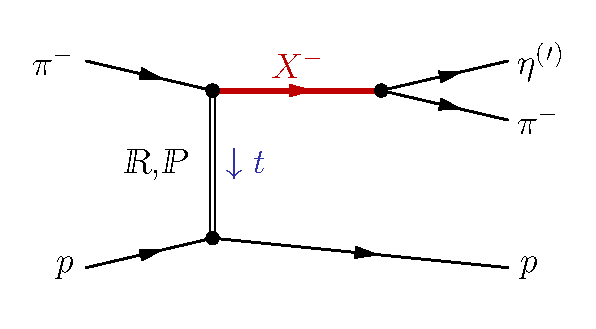
\includegraphics[width=0.5\textwidth]{diffractive_dissociation_x_etaprimepi_charged_p}%
  \caption{Diffractive scattering of a beam pion off a target proton
  mediated by Reggeon exchange.  In this scattering process, an
  intermediate state~$X^-$ with well-defined quantum numbers is
  produced, which in the example given here decays into the
  \etaOrPrPim channel.}%
  \label{fig:diffraction_etaprimepi}%
\end{figure}

The analysis is based on the measured intensity distribution, \ie the
number density of events, which is decomposed into partial-wave
amplitudes:\footnote{This is the simplest possible formula, were we
assume that the effect of the target spin is negligible and that all
partial wave amplitudes are fully coherent.}
\begin{equation}
  \label{eq:diffraction_intensity}
  \intensity(\Omega; w, t)
  = \frac{\dif{N}}{\dif{w}\, \dif{t}\, \dif{\Omega}}
  = \Abs[3]{\sum_{\ell m}^\infty \prodAmp_{\ell\, m}(w, t)\, Y_\ell^m(\Omega)}^2
  = \sum_{\substack{\ell m \\ \ell' m'}}^\infty Y_\ell^m(\Omega)\, \varrho^{\ell\, \ell'}_{m\, m'}(w, t)\, Y_{\ell'}^{m' *}(\Omega).
\end{equation}
Here, $N$~is the (acceptance-corrected) number of measured events,
$w$~is the invariant mass of the two-(pseudo)scalar system, $t$~is the
squared four-momentum transferred from the beam to the target
particle, and $\Omega = (\theta, \phi)$ is the direction of one of the
two (pseudo)scalar mesons the~$X$ decays into, measured in the
Gottfried-Jackson rest frame of~$X$.  The $\prodAmp_{\ell\, m}(w,
t)$ are the partial-wave amplitudes that correspond to an intermediate
state with a spin given by the relative orbital angular
momentum~$\ell$ between the two-(pseudo)scalar mesons and a spin
projection~$m$ \wrt the beam axis.  The partial-wave amplitudes form
the spin-density matrix of~$X$:
\begin{equation}
  \label{eq:diffraction_spin_dens_def}
  \varrho^{\ell\, \ell'}_{m\, m'}(w, t)
  = \prodAmp_{\ell\, m}(w, t)\, \prodAmp_{\ell'\, m'}^*(w, t),
\end{equation}
which by definition is Hermitian.  The angular distribution of the
$X$~decay products is given by the spherical harmonics
$Y_\ell^m(\Omega)$~\cite{wikipedia:sphericalHarm}, which are defined
by\footnote{See Eq.~(1) in Sec.~5.2 of
\refCite{Varshalovich:1988krb}.}
\begin{equation}
  \label{eq:spherical_harm_def}
  Y_\ell^m(\Omega)
  = \dUnderbrace{\sqrt{\frac{(2 \ell + 1)}{4 \pi}\, \frac{(\ell -m)!}{(\ell + m)!}}\, P_\ell^m(\cos\theta)}{= Y_\ell^m(\theta, 0)}\, e^{\imag\, m\, \phi},
\end{equation}
For convenience, we introduce the real-valued functions
\begin{equation}
  \label{eq:small_y_def}
  y_\ell^m(\theta)
  \equiv Y_\ell^m(\theta, 0)
  \quad\text{so that}\quad
  Y_\ell^m(\theta, \phi)
  = y_\ell^m(\theta)\, e^{\imag\, m\, \phi}.
\end{equation}
The spherical harmonics are special cases of the
$D$-functions~\cite{wikipedia:wignerD}, \ie\footnote{See Eq.~(37) in
Sec.~5.2.7 of \refCite{Varshalovich:1988krb}.}
\begin{equation}
  \label{eq:spherical_harm_wigner_d}
  Y_\ell^m(\Omega)
  = \sqrt{\frac{2 \ell + 1}{4 \pi}}\, D^{\ell *}_{m 0}(\phi, \theta, 0)
  \quad\text{and in particular}\quad
  y_\ell^m(\theta)
  = \sqrt{\frac{2 \ell + 1}{4 \pi}}\, d^\ell_{m 0}(\theta).
\end{equation}

In a partial-wave analysis, the partial-wave amplitudes
$\prodAmp_{\ell\, m}$, which contain the information about the
produced resonances~$X$, are determined by fitting the intensity model
in \cref{eq:diffraction_intensity} to the measured
$\Omega$~distribution in narrow $(w, t)$ cells.  Within each kinematic
cell, $\prodAmp_{\ell\, m}$ is treated as constant.  To simplify
notation, we hence will omit the~$w$ and $t$~dependencies in all
formulas below.

In addition to the partial-wave analysis, which decomposes the
\emph{amplitudes} into spherical harmonics, we can exploit the fact
that the $Y_\ell^m(\Omega)$ constitute a complete orthonormal set of
base functions on the surface of a unit sphere, \ie they fullfil the
completeness relation\footnote{See Eq.~(1) in Sec.~5.6.1 of
\refCite{Varshalovich:1988krb}.}
\begin{equation}
  \label{eq:spherical_harm_complete}
  \sum_{\ell m}^\infty Y_\ell^m(\Omega)\, Y_\ell^{m *}(\Omega')
  = \delta(\phi' - \phi)\, \delta(\theta' - \theta)
\end{equation}
and the orthonormality relation\footnote{%
Throughout the text, we use
\begin{equation}
  \int_{-1}^{+1}\!\!\! \dif{\cos\theta} \int_{-\pi}^{+\pi}\!\!\! \dif{\phi}
  = \int_{4 \pi}\!\!\! \dif{\Omega}.
\end{equation}
}\footnote{See Eq.~(2) in Sec.~5.6.1 of
\refCite{Varshalovich:1988krb}.}
\begin{equation}
  \label{eq:spherical_harm_orthonorm}
  \int_{4 \pi}\!\!\! \dif{\Omega}\, Y_\ell^m(\Omega)\, Y_{\ell'}^{m' *}(\Omega)
  = \delta_{\ell \ell'}\, \delta_{m m'},
\end{equation}
and instead decompose the \emph{intensity} into spherical harmonics.

Using \cref{eq:gen_fourier_series,eq:expansion_coefficient} we
obtain:\footnote{The expansion into a series of spherical harmonics is
also referred to as Laplace series~\cite{MathWorld:LaplaceSeries}.}
\begin{equation}
  \label{eq:diffraction_intensity_moments}
  \intensity(\Omega)
  = \sum_{L M}^\infty H(L, M)\, Y_L^M(\Omega),
\end{equation}
with the moments\footnote{Note that in
\cref{sec:diffraction:moments_norm}, we will introduce a different
normalization for $H(L, M)$ (see \cref{eq:diffraction_moments_norm}).}
\begin{equation}
  \label{eq:diffraction_moments}
  H(L, M)
  = \int_{4 \pi}\!\!\! \dif{\Omega}\, \intensity(\Omega)\, Y_L^{M *}(\Omega).
\end{equation}
It is important to note that although
\cref{eq:diffraction_intensity_moments} and
\cref{eq:diffraction_intensity} use the same basis functions, the two
represent different decompositions.  In
\cref{eq:diffraction_intensity} the amplitudes are decomposed into
spherical harmonics, \ie partial-wave amplitudes, whereas in
\cref{eq:diffraction_intensity_moments} the intensity is decomposed.
Whereas the former decomposition is based on a physics model of the
reaction, the moment decomposition is purely mathematical.  An
advantage of the moment decomposition is that it is unique, whereas
the partial-wave decomposition may have mathematical as well as
statistical ambiguities (see \eg\ \refCite{Chung:1997qd}).  Another
advantage of the moment decomposition is that the moments can be
rather easily calculated from the data, which will be discussed in
\cref{sec:diffraction:moments_data}.  The downside of this approach is
that the physics interpretation of the moments is difficult because
they are only indirectly related to the partial-wave amplitudes.  This
will be discussed in more detail in \cref{sec:diffraction:moments_pw}.


\subsection{Relation between moments and partial-wave amplitudes}%
\label{sec:diffraction:moments_pw}

In order to relate the partial-wave amplitudes~$\prodAmp_{\ell\,
m}$ and the moments~$H(L, M)$ we express the moments in terms of
spin-density elements using the relation\footnote{See Eq.~(A.15) in
\refCite{Chung:1971ri}.}
\begin{equation}
  \label{eq:spherical_harm_prod}
  Y_{\ell'}^{m' *}(\Omega)\, Y_{\ell}^m(\Omega)
  = \sum_{L M}^\infty \sqrt{\frac{2 L + 1}{4 \pi}}\, \sqrt{\frac{2 \ell' + 1}{2 \ell + 1}}\, \clebsch{\ell'}{0}{L}{0}{\ell}{0}\, \clebsch{\ell'}{m'}{L}{M}{\ell}{m}\, Y_L^M(\Omega).
\end{equation}
Here, \clebsch{j_1}{m_1}{j_2}{m_2}{J}{M} are the Clebsch-Gordan
coefficients for the coupling of the spin states $\ket{j_1\; m_1}$
and~$\ket{j_2\; m_2}$ to $\ket{J\; M}$.  Note that the Clebsch-Gordan
coefficient \clebsch{\ell'}{0}{L}{0}{\ell}{0} requires
that\footnote{See Eq.~(32) in Sec.~8.5.2 of
\refCite{Varshalovich:1988krb}.}
\begin{equation}
  \label{eq:ang_mom_sum}
  \ell' + L + \ell
  = \text{even}.
\end{equation}
Inserting \cref{eq:spherical_harm_prod} into
\cref{eq:diffraction_intensity}, yields
\begin{equation}
  \intensity(\Omega)
  = \sum_{L M}^\infty \sqrt{\frac{2 L + 1}{4 \pi}} \sum_{\substack{\ell m \\ \ell' m'}}^\infty
  \sqrt{\frac{2 \ell' + 1}{2 \ell + 1}}\, \clebsch{\ell'}{0}{L}{0}{\ell}{0}\, \clebsch{\ell'}{m'}{L}{M}{\ell}{m}\,
  \varrho^{\ell\, \ell'}_{m\, m'}\, Y_L^M(\Omega).
\end{equation}
Comparing with \cref{eq:diffraction_intensity_moments}, we see
that\footnote{Note that in \cref{sec:diffraction:moments_norm}, we
will introduce a different normalization for $H(L, M)$ (see
\cref{eq:diffraction_moments_pw_norm}).}
\begin{equation}
  \label{eq:diffraction_moments_pw}
  H(L, M)
  = \sqrt{\frac{2 L + 1}{4 \pi}} \sum_{\substack{\ell m \\ \ell' m'}}^\infty
  \sqrt{\frac{2 \ell' + 1}{2 \ell + 1}}\,
  \clebsch{\ell'}{0}{L}{0}{\ell}{0}\, \clebsch{\ell'}{m'}{L}{M}{\ell}{m}\,
  \varrho^{\ell\, \ell'}_{m\, m'}.
\end{equation}

It is important to note that we can always calculate all moments from
a given set of partial-wave amplitudes using
\cref{eq:diffraction_moments_pw}.  However, in general the converse is
not true because there are unphysical sets of moments that do not
correspond to a partial-wave decomposition and even for a physical set
of moments we need to solve a system of quadratic equations in the
partial-wave amplitudes given by
\cref{eq:diffraction_moments_pw,eq:diffraction_spin_dens_def}, which
may contain ambiguities.

From \cref{eq:diffraction_moments_pw} it is clear that the moments are
linear combinations of spin-density matrix elements, \ie of
intensities and interference terms of the partial-wave amplitudes
$\prodAmp_{\ell\, m}$.  The equation also shows that~$L$ and~$M$
are only indirectly linked to the physical angular momentum quantum
numbers of the two-body system.  For given~$L$, the Clebsch-Gordan
coefficients limit the sum to those partial waves, for which $\ell' +
L + \ell = \text{even}$ (see \cref{eq:ang_mom_sum}), $\abs{\ell' - L}
\leq \ell \leq \ell' + L$, and $m = m' + M$.  This means that if the
partial-wave amplitudes vanish for $\ell, \ell' > \ell_\text{max}$ the
moments~$H(L, M)$ will vanish $L > 2 \ell_\text{max}$.

Alternatively, we can derive \cref{eq:diffraction_moments_pw} by
inserting \cref{eq:diffraction_intensity} into
\cref{eq:diffraction_moments} and using\footnote{This is the complex
conjugate of Eq.~(4) in Sec.~5.9.1 of \refCite{Varshalovich:1988krb}.}
\begin{equation}
  \label{eq:spherical_harm_clebsch}
  \int_{4 \pi}\!\!\! \dif{\Omega}\,
  Y_{\ell'}^{m' *}(\Omega)\, Y_L^{M *}(\Omega)\, Y_{\ell}^m(\Omega)
  = \sqrt{\frac{2 \ell' + 1}{4 \pi}}\, \sqrt{\frac{2 L + 1}{2 \ell + 1}}\, \clebsch{\ell'}{0}{L}{0}{\ell}{0}\, \clebsch{\ell'}{m'}{L}{M}{\ell}{m}.
\end{equation}
Doing so, we obtain
\begin{equation}
  H(L, M)
  = \sum_{\substack{\ell m \\ \ell' m'}}^\infty
  \varrho^{\ell\, \ell'}_{m\, m'}\,
  \int_{4 \pi}\!\!\! \dif{\Omega}\,
  Y_\ell^m(\Omega)\,
  Y_{\ell'}^{m' *}(\Omega)\,
  Y_L^{M *}(\Omega),
\end{equation}
which is equivalent to \cref{eq:diffraction_moments_pw}.


\subsection{Normalization of moments}%
\label{sec:diffraction:moments_norm}

In order to derive a more practical normalization of the moments, it
is instructive to look at the lowest moment $H(0, 0)$, which is a
special case.  With
\cref{eq:diffraction_moments,eq:diffraction_moments_pw},
$Y_0^0(\Omega) = 1 / \sqrt{4 \pi}$, and
\begin{equation}
  \clebsch{\ell'}{m'}{0}{0}{\ell}{m}
  = \delta_{\ell \ell'}\, \delta_{m m'}
\end{equation}
we get
\begin{equation}
  H(0, 0)
  = \frac{1}{\sqrt{4 \pi}}\, \int_{4 \pi}\!\!\! \dif{\Omega}\, \intensity(\Omega)
  = \sqrt{\frac{2 L + 1}{4 \pi}} \sum_{\substack{\ell m \\ \ell' m'}}^\infty \varrho^{\ell\, \ell}_{m\, m}.
\end{equation}
This means, up to a factor of $1 / \sqrt{4 \pi}$, $H(0, 0)$ is the
integral of the intensity over the phase space, which is identical to
the sum of all partial-wave intensities.

In order to make $H(0, 0)$ identical to the intensity integral and the
sum of all partial-wave intensities, it is customary to change the
normalization of the moments using the replacement
\begin{equation}
  H(L, M)
  \to \sqrt{\frac{4 \pi}{2 L + 1}}\, H(L, M).
\end{equation}
Applying the above,
\cref{eq:diffraction_intensity_moments,eq:diffraction_moments} become
\begin{equation}
  \label{eq:diffraction_intensity_moments_norm}
  \intensity(\Omega)
  = \sum_{L M}^\infty \sqrt{\frac{2 L + 1}{4 \pi}}\, H(L, M)\, Y_L^M(\Omega),
\end{equation}
and
\begin{equation}
  \label{eq:diffraction_moments_norm}
  H(L, M)
  = \sqrt{\frac{4 \pi}{2 L + 1}}\, \int_{4 \pi}\!\!\! \dif{\Omega}\, \intensity(\Omega)\, Y_L^{M *}(\Omega).
\end{equation}
Using the relation between the spherical harmonics and the Wigner
$D$-functions in \cref{eq:spherical_harm_wigner_d},
\cref{eq:diffraction_intensity_moments_norm,eq:diffraction_moments_norm}
become identical to Eqs.~(6) and~(9) in \refCite{Chung:1997qd}.

Similarly, \cref{eq:diffraction_moments_pw} becomes
\begin{equation}
  \label{eq:diffraction_moments_pw_norm}
  H(L, M)
  = \sum_{\substack{\ell m \\ \ell' m'}}^\infty
  \sqrt{\frac{2 \ell' + 1}{2 \ell + 1}}\,
  \clebsch{\ell'}{0}{L}{0}{\ell}{0}\, \clebsch{\ell'}{m'}{L}{M}{\ell}{m}\,
  \varrho^{\ell\, \ell'}_{m\, m'}.
\end{equation}

For the remainder of this section we will use the moments defined in
\cref{eq:diffraction_intensity_moments_norm,eq:diffraction_moments_norm,eq:diffraction_moments_pw_norm}, for which in particular
\begin{equation}
  \label{eq:diffraction_moment_00_pw}
  H(0, 0)
  = \int_{4 \pi}\!\!\! \dif{\Omega}\, \intensity(\Omega)
  = \sum_{\substack{\ell m \\ \ell' m'}}^\infty \varrho^{\ell\, \ell}_{m\, m}.
\end{equation}


\subsection{Symmetry properties of moments}%
\label{sec:diffraction:moments_sym}

Since the moments are defined by the spherical harmonics (see
\cref{eq:diffraction_moments_norm}), they inherit the symmetry properties
of the spherical harmonics.  From\footnote{See Eq.~(1) in Sec.~5.4 of
\refCite{Varshalovich:1988krb}.}
\begin{equation}
  \label{eq:spherical_harm_sym}
  Y_L^{M *}(\Omega)
  = (-1)^M\, Y_L^{(-M)}(\Omega)
\end{equation}
it follows that
\begin{equation}
  \label{eq:diffraction_moment_sym_1}
  H^*(L, M)
  = \sqrt{\frac{4 \pi}{2 L + 1}}\, \int_{4 \pi}\!\!\! \dif{\Omega}\, \intensity(\Omega)\, Y_L^M(\Omega)
  = (-1)^M \sqrt{\frac{4 \pi}{2 L + 1}}\, \int_{4 \pi}\!\!\! \dif{\Omega}\, \intensity(\Omega)\, Y_L^{(-M) *}(\Omega)
  = (-1)^M\, H(L, -M).
\end{equation}

Alternatively, we can derive \cref{eq:diffraction_moment_sym_1} by
using \cref{eq:diffraction_moments_pw_norm} plus the fact that the
spin-density matrix is Hermitian,
\ie
\begin{equation}
  \rBrk[1]{\varrho^{\ell\, \ell'}_{m\, m'}}^*
  = \varrho^{\ell'\, \ell}_{m'\, m},
\end{equation}
and that the Clebsch-Gordan coefficients have the symmetry
property\footnote{See Eq.~(10) in Sec.~8.4.3 of
\refCite{Varshalovich:1988krb}.}
\begin{equation}
  \label{eq:clebsch_sym}
  \clebsch{\ell'}{m'}{L}{M}{\ell}{m}
  = \rdUnderbrace{(-1)^{\ell' + L - \ell}}{\equalUsing{$\mathclap{\text{\cref{eq:ang_mom_sum}}}$}\quad 1}\,
  \clebsch{L}{M}{\ell'}{m'}{\ell}{m}
  = (-1)^{L - M}\, \sqrt{\frac{2 \ell + 1}{2 \ell' + 1}}\, \clebsch{\ell}{m}{L}{-M}{\ell'}{m'}.
\end{equation}
Doing so, we get
\begin{align}
  H^*(L, M)
  ={}& \sum_{\substack{\ell m \\ \ell' m'}}^\infty
    \sqrt{\frac{2 \ell' + 1}{2 \ell + 1}}\,
    (-1)^{L - 0}\, \sqrt{\frac{2 \ell + 1}{2 \ell' + 1}}\, \clebsch{\ell}{0}{L}{0}{\ell'}{0}\,
    (-1)^{L - M}\, \sqrt{\frac{2 \ell + 1}{2 \ell' + 1}}\, \clebsch{\ell}{m}{L}{-M}{\ell'}{m'}\,
    \varrho^{\ell'\, \ell}_{m'\, m} \nonumber
  \\
  ={}& \dUnderbrace{(-1)^{2 L - M}}{= (-1)^M}
  \sum_{\substack{\ell m \\ \ell' m'}}^\infty
  \sqrt{\frac{2 \ell + 1}{2 \ell' + 1}}\,
  \clebsch{\ell}{0}{L}{0}{\ell'}{0}\, \clebsch{\ell}{m}{L}{-M}{\ell'}{m'}\,
  \varrho^{\ell'\, \ell}_{m'\, m}
  \\
  \equalUsing{$\mathclap{\substack{\displaystyle{\ell \leftrightarrow \ell'} \\ \displaystyle{m \leftrightarrow m'}}}$}{}& \quad
  (-1)^M\, H(L, -M),
\end{align}
where in the last step we rearranged the terms in the sum and compared
to \cref{eq:diffraction_moments_pw_norm}.

The symmetry relation in \cref{eq:diffraction_moment_sym_1} ensures
that the intensity function in
\cref{eq:diffraction_intensity_moments_norm} is real-valued:
\begin{flalign}
  \intensity(\Omega)
  ={}& \sum_{L = 0}^\infty \sum_{M = -L}^{+L} \sqrt{\frac{2 L + 1}{4 \pi}}\, H(L, M)\, Y_L^M(\Omega) && \nonumber
  \\
  ={}& \sum_{L = 0}^\infty \sqrt{\frac{2 L + 1}{4 \pi}} \sBrk[4]{\rdUnderbrace{\sum_{M = -L}^{-1} H(L, M)\, Y_L^M(\Omega)}%
    {= \sum_{M = +1}^{+L} H(L, -M)\, Y_L^{(-M)}(\Omega)
    \equalUsingTwo{\cref{eq:spherical_harm_sym}}{\cref{eq:diffraction_moment_sym_1}} (-1)^M\, H^*(L, M)\, (-1)^M\, Y_L^{M *}(\Omega)}
    + H(L, 0)\, Y_L^0(\Omega) + \sum_{M = +1}^{+L} H(L, M)\, Y_L^M(\Omega)} && \nonumber
  \\
  ={}& \sum_{L = 0}^\infty \sqrt{\frac{2 L + 1}{4 \pi}} \sBrk[4]{H(L, 0)\, Y_L^0(\Omega) + \sum_{M = +1}^{+L}
  \rdUnderbrace{\cBrk{H(L, M)\,Y_L^M(\Omega) + H^*(L, M)\,Y_L^{M *}(\Omega)}}{= 2 \Re{H(L, M)\, Y_L^M(\Omega)}}} && \nonumber
  \\
  \label{eq:diffraction_intensity_moments_general}
  ={}& \sum_{L = 0}^\infty \sqrt{\frac{2 L + 1}{4 \pi}} \sum_{M = 0}^{L} (2 - \delta_{M 0})\, \Re{H(L, M)\, Y_L^M(\Omega)}. &&
\end{flalign}
For the last step, we have used that $Y_L^0(\Omega)$ and hence also
$H(L, 0)$ are real-valued by construction.  Due to the above, we only
have to calculate the moments with $M \geq 0$.

In addition to the symmetry properties of the spherical harmonics, we
can also exploit the symmetry properties of the $X$~spin-density
matrix.  Since the scattering process is invariant under parity, we
have\footnote{See Eq.~2.7 in \refCite{Chung:1974fq}.}
\begin{equation}
  \label{eq:diffraction_spin_dens_parity_general}
  \varrho^{\ell\, \ell'}_{m\, m'}
  = P\, P'\, (-1)^{\ell - \ell'}\, (-1)^{m - m'}\, \varrho^{\ell'\, \ell}_{{-m}\, {-m'}}.
\end{equation}
Here $\ell^P$ and $(\ell')^{P'}$ are two spin-parity states of~$X$.
For the two-body decay $X \to 1 + 2$, the intrinsic parity of~$X$ is
given by
\begin{equation}
  P
  = P_1\, P_2\, (-1)^\ell.
\end{equation}
Assuming that $X$~decays into two daughter particles with identical
parity, \eg two pseudoscalars such as $\etaOrPr \pi$,
\cref{eq:diffraction_spin_dens_parity_general} simplifies to
\begin{equation}
  \label{eq:diffraction_spin_dens_parity}
  \varrho^{\ell\, \ell'}_{m\, m'}
  = (-1)^{m - m'}\, \varrho^{\ell'\, \ell}_{{-m}\, {-m'}}.
\end{equation}

Using this together with
\cref{eq:diffraction_moments_pw_norm} and the symmetry
property\footnote{See Eq.~(11) in Sec.~8.4.3 of
\refCite{Varshalovich:1988krb}.}
\begin{equation}
  \label{eq:clebsch_sym2}
  \clebsch{\ell'}{m'}{L}{M}{\ell}{m}
  = \rdUnderbrace{(-1)^{\ell' + L - \ell}}{\equalUsing{$\mathclap{\text{\cref{eq:ang_mom_sum}}}$}\quad 1}\,
  \clebsch{\ell'}{-m'}{L}{-M}{\ell}{-m}
\end{equation}
of the Clebsch-Gordan coefficients, we get
\begin{align}
  H(L, -M)
  ={}& \sum_{\substack{\ell m \\ \ell' m'}}^\infty
  \sqrt{\frac{2 \ell' + 1}{2 \ell + 1}}\,
  \clebsch{\ell'}{0}{L}{0}{\ell}{0}\, \clebsch{\ell'}{-m'}{L}{M}{\ell}{-m}\,
  (-1)^{m - m'}\, \varrho^{\ell\, \ell'}_{{-m}\, {-m}'} \nonumber
  \\
  \label{eq:diffraction_moment_sym_2}
  \equalUsing{$\mathclap{\substack{\displaystyle{m \to -m} \\ \displaystyle{m' \to -m'}}}$}{}& \quad
  (-1)^M\, H(L, M),
\end{align}
where in the last step, we used that the second Clebsch-Gordan
coefficient enforces $m' - M = m$,\footnote{Therefore, $(-1)^{m - m'}
= (-1)^{m' - m} = (-1)^M$.} rearranged the terms in the sum, and
compared to \cref{eq:diffraction_moments_pw_norm}.

From \cref{eq:diffraction_moment_sym_1,eq:diffraction_moment_sym_2} follows that
\begin{equation}
  \label{eq:diffraction_moment_real}
  H(L, M)
  = H^*(L, M),
\end{equation}
\ie all moments must be real-valued.  Inserting
\cref{eq:small_y_def,eq:diffraction_moments_norm} on both sides, we
obtain
\begin{align}
  \sqrt{\frac{4 \pi}{2 L + 1}}\, \int_{4 \pi}\!\!\! \dif{\Omega}\, \intensity(\Omega)\, Y_L^{M *}(\Omega)
  \mustBeEq{}&
  \sqrt{\frac{4 \pi}{2 L + 1}}\, \int_{4 \pi}\!\!\! \dif{\Omega}\, \intensity(\Omega)\, Y_L^M(\Omega) \\
  \sqrt{\frac{4 \pi}{2 L + 1}}\, \int_{4 \pi}\!\!\! \dif{\Omega}\, \intensity(\Omega)\, y_L^M(\theta) \sBrk{\cos(M \phi) - \imag \sin(M \phi)}
  \mustBeEq{}&
  \sqrt{\frac{4 \pi}{2 L + 1}}\, \int_{4 \pi}\!\!\! \dif{\Omega}\, \intensity(\Omega)\, y_L^M(\theta) \sBrk{\cos(M \phi) + \imag \sin(M \phi)}.
\end{align}
Consequently,
\begin{align}
  \label{eq:diffraction_moments_real}
  H(L, M)
  ={}& \sqrt{\frac{4 \pi}{2 L + 1}}\, \int_{4 \pi}\!\!\! \dif{\Omega}\, \intensity(\Omega)\, y_L^M(\theta)\, \cos(M\, \phi)
  \intertext{and}
  \label{eq:diffraction_moments_imag}
  0
  ={}& \sqrt{\frac{4 \pi}{2 L + 1}}\, \int_{4 \pi}\!\!\! \dif{\Omega}\, \intensity(\Omega)\, y_L^M(\theta)\, \sin(M\, \phi).
\end{align}

We can also rewrite \cref{eq:diffraction_intensity_moments_general}:
\begin{align}
  \intensity(\Omega)
  ={}& \sum_{L = 0}^\infty \sqrt{\frac{2 L + 1}{4 \pi}} \sum_{M = 0}^{L} (2 - \delta_{M 0})\, H(L, M)\, \Re{Y_L^M(\Omega)} \nonumber
  \\
  \label{eq:diffraction_intensity_moments_real}
  ={}& \sum_{L = 0}^\infty \sqrt{\frac{2 L + 1}{4 \pi}} \sum_{M = 0}^{L} (2 - \delta_{M 0})\, H(L, M)\, y_L^M(\theta)\, \cos(M\, \phi).
\end{align}
This is identical to Eq.~(13) in \refCite{Chung:1997qd}.


\subsection{Reflectivity basis}%
\label{sec:diffraction:reflectivity}

It is often advantageous to express the intensity distribution in
\cref{eq:diffraction_intensity} in the reflectivity basis, \ie using
the reflectivity states of~$X$
\begin{equation}
  \label{eq:diffraction_refl_def}
  \ket{\refl, \ell, m}
  \equiv \mathcal{N}_m \sBrk[2]{\ket{\ell, m} - \refl\, (-1)^m\, \ket{\ell, {-m}}},
\end{equation}
which are eigenstates of the reflection operator~$\Pi_y$ through the
production plane that is spanned by the momenta of the beam particle
and~$X$.  The relative sign of the terms in
\cref{eq:diffraction_refl_def} has been chosen such that for a
pseudoscalar beam particle the eigenvalues~$\refl = \pm$ of~$\Pi_y$,
\ie the \emph{reflectivities}, correspond to the \emph{naturality} of
the exchange particle in the scattering process.  The normalization
factor
\begin{equation}
  \label{eq:refl_norm}
  \mathcal{N}_m
  = \begin{cases*}
      1 / \sqrt{2} & for $m > 0$, \\
      1 / 2        & for $m = 0$, \\
      0            & for $m < 0$
    \end{cases*}
\end{equation}
ensures that the multiplicity of $2 \ell + 1$ of the spin states is
conserved by constraining~$m$ to be non-negative.  It is important to
note that the definition in \cref{eq:diffraction_refl_def} forbids
positive-reflectivity states with $m = 0$.

The reflectivity basis is implemented by introducing the functions
\begin{equation}
  \label{eq:diffraction_spherical_harm_refl}
  \prescript{(\refl)}{}{Y}_\ell^m(\Omega)
  \equiv \mathcal{N}_m \sBrk[2]{Y_\ell^m(\Omega) - \refl\, (-1)^m\, Y_\ell^{(-m)}(\Omega)}.
\end{equation}
Note that with \cref{eq:spherical_harm_sym} and the definition of the
spherical harmonics in \cref{eq:spherical_harm_def,eq:small_y_def}, it
follows from \cref{eq:diffraction_spherical_harm_refl} that
\begin{equation}
  \prescript{(+)}{}{Y}_\ell^m(\Omega)
  = 2 \imag\, \mathcal{N}_m\, y_\ell^m(\theta)\, \sin(m\, \phi)
  \quad\text{and}\quad
  \prescript{(-)}{}{Y}_\ell^m(\Omega)
  = 2 \mathcal{N}_m\, y_\ell^m(\theta)\, \cos(m\, \phi),
\end{equation}
\ie $\prescript{(+)}{}{Y}_\ell^m(\Omega)$ is purely imaginary and
$\prescript{(-)}{}{Y}_\ell^m(\Omega)$ purely real.

Replacing $Y_\ell^m(\Omega)$ in \cref{eq:diffraction_intensity} by
\cref{eq:diffraction_spherical_harm_refl} and using the fact that
amplitudes with opposite reflectivities do not interfere, we obtain
\begin{equation}
  \label{eq:diffraction_intensity_refl}
  \intensity(\Omega)
  = \sum_{\refl = \pm} \Abs[3]{\sum_{\ell m}^\infty \prescript{(\refl)}{}{\prodAmp}_{\!\ell\, m}\, \prescript{(\refl)}{}{Y}_\ell^m(\Omega)}^2
  = \sum_{\refl = \pm} \sum_{\substack{\ell m \\ \ell' m'}}^\infty
  \prescript{(\refl)}{}{Y}_\ell^m(\Omega)\, \prescript{(\refl)}{}{\varrho}^{\ell\, \ell'}_{m\, m'}\, \prescript{(\refl)}{}{Y}_{\ell'}^{m' *}(\Omega),
\end{equation}
where we have introduced the spin-density matrix of~$X$,
\begin{equation}
  \label{eq:diffraction_refl_spin-dens}
  \prescript{(\refl)}{}{\varrho}^{\ell\, \ell'}_{m\, m'}
  = \prescript{(\refl)}{}{\prodAmp}_{\!\ell\, m}\, \prescript{(\refl)}{}{\prodAmp}_{\!\ell'\, m'}^*,
\end{equation}
in the reflectivity basis analogous to
\cref{eq:diffraction_spin_dens_def}.

In order to relate the partial-wave
amplitudes~$\prescript{(\refl)}{}{\prodAmp}_{\!\ell\, m}$ and the
moments~$H(L, M)$ we insert \cref{eq:diffraction_spherical_harm_refl}
into \cref{eq:diffraction_intensity_refl} and use
\cref{eq:spherical_harm_prod}:
\begin{align}
  \intensity(\Omega)
  ={}&
    \sum_{\refl = \pm} \sum_{\substack{\ell m \\ \ell' m'}}^\infty
    \prescript{(\refl)}{}{\varrho}^{\ell\, \ell'}_{m\, m'}\,
    \mathcal{N}_m\, \mathcal{N}_{m'}
    \sBrk[2]{Y_\ell^m(\Omega) - \refl\, (-1)^m\, Y_\ell^{(-m)}(\Omega)}
    \sBrk[2]{Y_{\ell'}^{m' *}(\Omega) - \refl\, (-1)^{m'}\, Y_{\ell'}^{(-m') *}(\Omega)}
  \\
  ={}& \begin{multlined}[t][0.85\columnwidth]
    \sum_{\refl = \pm} \sum_{\substack{\ell m \\ \ell' m'}}^\infty
    \prescript{(\refl)}{}{\varrho}^{\ell\, \ell'}_{m\, m'}\,
    \sum_{L M}^\infty \sqrt{\frac{2 L + 1}{4 \pi}}\, \sqrt{\frac{2 \ell' + 1}{2 \ell + 1}}\, \clebsch{\ell'}{0}{L}{0}{\ell}{0} \\
    \shoveleft{\times \mathcal{N}_m\, \mathcal{N}_{m'}\, \Big[ \clebsch{\ell'}{m'}{L}{M}{\ell}{m}                       - \refl\, (-1)^{m'}\, \clebsch{\ell'}{-m'}{L}{M}{\ell}{m}} \\
      - \refl\, (-1)^m\, \clebsch{\ell'}{m'}{L}{M}{\ell}{-m} + (-1)^{m + m'}\, \clebsch{\ell'}{-m'}{L}{M}{\ell}{-m} \Big]\,
    Y_L^M(\Omega).
  \end{multlined}
\end{align}
We rewrite the last Clebsch-Gordan coefficient in the square bracket
using the symmetry relation in \cref{eq:clebsch_sym2} and the fact
that $(-1)^{m + m'} = (-1)^{2m}\, (-1)^{m' - m} = (-1)^M$ because this
Clebsch-Gordan coefficient enforces that $m' - M = m$.  With this we
arrive at
\begin{multline}
  \intensity(\Omega)
  = \sum_{L M}^\infty \sqrt{\frac{2 L + 1}{4 \pi}}
  \sum_{\refl = \pm} \sum_{\substack{\ell m \\ \ell' m'}}^\infty
  \mathcal{N}_m\, \mathcal{N}_{m'}\,
  \sqrt{\frac{2 \ell' + 1}{2 \ell + 1}}\,
  \clebsch{\ell'}{0}{L}{0}{\ell}{0}
  \\
  \times \Big[
    \clebsch{\ell'}{m'}{L}{M}{\ell}{m}
    + (-1)^M\, \clebsch{\ell'}{m'}{L}{-M}{\ell}{m} \\
    - \refl\, (-1)^{m'}\, \clebsch{\ell'}{-m'}{L}{M}{\ell}{m}
    - \refl\, (-1)^m\, \clebsch{\ell'}{m'}{L}{M}{\ell}{-m} \Big]
  \prescript{(\refl)}{}{\varrho}^{\ell\, \ell'}_{m\, m'}\,
  Y_L^M(\Omega).
\end{multline}
Comparing with \cref{eq:diffraction_intensity_moments_norm} we see
that
\begin{multline}
  \label{eq:diffraction_moments_pw_refl_norm}
  H(L, M)
  = \sum_{\refl = \pm} \sum_{\substack{\ell m \\ \ell' m'}}^\infty
  \mathcal{N}_m\, \mathcal{N}_{m'}\,
  \sqrt{\frac{2 \ell' + 1}{2 \ell + 1}}\,
  \clebsch{\ell'}{0}{L}{0}{\ell}{0} \\
  \times \Big[
    \clebsch{\ell'}{m'}{L}{M}{\ell}{m}
    + (-1)^M\, \clebsch{\ell'}{m'}{L}{-M}{\ell}{m} \\
    - \refl\, (-1)^{m'}\, \clebsch{\ell'}{-m'}{L}{M}{\ell}{m}
    - \refl\, (-1)^m\, \clebsch{\ell'}{m'}{L}{M}{\ell}{-m} \Big]
  \prescript{(\refl)}{}{\varrho}^{\ell\, \ell'}_{m\, m'},
\end{multline}
which is identical to Eqs.~(29) and~(31) in \refCite{Chung:1997qd}.
It is important to note that each moment is an incoherent sum of
contributions from both reflectivities, \ie the moments do not
separate these contributions.
\Cref{eq:diffraction_moments_pw_refl_norm} is the equivalent of
\cref{eq:diffraction_moments_pw_norm} in the reflectivity basis.

Using the above, we can calculate the lowest moment in the
reflectivity basis:
\begin{align}
  H(0, 0)
  ={}& \begin{multlined}[t]
    \sum_{\refl = \pm} \sum_{\substack{\ell m \\ \ell' m'}}^\infty
    \sqrt{\frac{2 \ell' + 1}{2 \ell + 1}}\,
    \delta_{\ell \ell'}
    \\
    \times \rdUnderbrace{\mathcal{N}_m\, \mathcal{N}_{m'} \sBrk[2]{%
      \delta_{\ell \ell'}\, \delta_{m m'}
      + \delta_{\ell \ell'}\, \delta_{m m'}
      - \refl\, (-1)^{m'}\, \delta_{\ell \ell'}\, \delta_{m (-m')}
      - \refl\, (-1)^m\, \delta_{\ell \ell'}\, \delta_{(-m) m'}}}%
      {= \delta_{\ell \ell'}\, \delta_{m m'} \times
      \begin{cases*}
        \frac{1}{2}\, (1 + 1)                 & for $m > 0$, \\
        \frac{1}{4}\, (1 + 1 - \refl - \refl) & for $m = 0$
      \end{cases*}}
    \prescript{(\refl)}{}{\varrho}^{\ell\, \ell'}_{m\, m'}
  \end{multlined} \nonumber
  \\
  \label{eq:diffraction_moment_00_pw_refl}
  ={}& \sum_{\refl = \pm} \sum_\ell^\infty \sum_{m = 0}^\ell \prescript{(\refl)}{}{\varrho}^{\ell\, \ell}_{m\, m},
\end{align}
where we have inserted the normalization factor from
\cref{eq:refl_norm}, which removes all terms with $m < 0$ or $m' < 0$.
As expected, $H(0, 0)$ is the sum of all partial-wave intensities,
equivalent to \cref{eq:diffraction_moment_00_pw}.


\subsection{Calculation of moments from data}%
\label{sec:diffraction:moments_data}

\subsubsection{Ideal detector with perfect acceptance}%
\label{sec:diffraction:moments_data_no_acc}

Using \cref{eq:diffraction_moments_real}, we can calculate the
real-valued moments $H(L, M)$ with $M \geq 0$ from an intensity
distribution~$\intensity(\Omega)$.  The moments with $M < 0$ can be
calculated from the moments with $M \geq 0$ using
\cref{eq:diffraction_moment_sym_2}.  Assuming an ideal detector with
perfect acceptance, the measured events will follow the distribution
$\intensity(\Omega)$.  For a data sample with $N$~events, the best
estimates $\hat{H}(L, M)$ for the moments are hence given by replacing
the integral over $\intensity(\Omega)$ in
\cref{eq:diffraction_moments_real} by a sum over the measured events,
\ie
\begin{equation}
  \label{eq:diffraction_moments_estimate}
  \hat{H}(L, M)
  = \sum_{i = 1}^N \sqrt{\frac{4 \pi}{2 L + 1}}\, y_L^M(\theta_i)\, \cos(M\, \phi_i)
  \equiv \sum_{i = 1}^N f_{L M}(\Omega_i),
\end{equation}
where~$\theta_i$ and~$\phi_i$ are the angles measured for event~$i$.
Here, we have omitted the $4 \pi / N$ factor that one would normally
write when estimating an integral over the surface of the unit sphere.
In the literature, this is referred to as \emph{unnormalized
moments}\footnote{This is somewhat of a misnomer because also the
unnormalized moments have a well-defined normalization.  However, the
normalization is not absolute and hence these moments depend on the
number of events.} and with the chosen normalization (see
\cref{sec:diffraction:moments_norm}) it leads to
\begin{equation}
  \label{eq:diffraction_norm_00}
  H(0, 0)
  = N
  \quad\text{because}\quad
  f_{00}(\Omega)
  = 1
  = \text{const}.
\end{equation}
\todo{relate to \cref{eq:diffraction_moment_00_pw}? Why no
interference effect? integral of interference terms always 0?}This
means that unnormalized moments are expressed in units of events.

In practice, events are often weighted to statistically subtract
backgrounds.  To take these weights into account, we extend
\cref{eq:diffraction_moments_estimate}:
\begin{equation}
  \label{eq:diffraction_moments_estimate_weighted}
  \hat{H}(L, M)
  = \sum_{i = 1}^N w_i\, f_{L M}(\Omega_i).
\end{equation}
Here, we assume that the event weights~$w_i$ are normalized such that
\begin{equation}
  \label{eq:event_weights_norm}
  \sum_{i = 1}^N w_i
  = N_\text{sub}
  = H(0, 0)
\end{equation}
with $N_\text{sub}$~being the number of events after the background
subtraction.  Note that for unweighted events $w_i = 1~ \forall i$.

To estimate the covariances of the $\hat{H}(L, M)$, we assume that the
event weights are constants and exploit that the events are
statistically independent and identically distributed according to
$\intensity(\Omega)$.  The covariance of two moments is therefore
\begin{align}
  \cov[1]{\hat{H}(L, M), \hat{H}(L', M')}
  ={}& \cov[4]{\sum_{i = 1}^N w_i\, f_{L M}(\Omega_i), \sum_{j = 1}^N w_j\, f_{L' M'}(\Omega_j)} \nonumber
  \\
  ={}& \exptVal[4]{\sum_{i, j = 1}^N w_i\, w_j\, f_{L M}(\Omega_i)\, f_{L' M'}(\Omega_j)}
     - \exptVal[4]{\sum_{i = 1}^N w_i\, f_{L M}(\Omega_i)}\, \exptVal[4]{\sum_{j = 1}^N w_j\, f_{L' M'}(\Omega_j)} \nonumber
  \\
  ={}& \sum_{i, j = 1}^N w_i\, w_j \rBrk[2]{\exptVal[1]{f_{L M}(\Omega_i)\, f_{L' M'}(\Omega_j)}
                                       - \exptVal[1]{f_{L M}(\Omega_i)}\, \exptVal[1]{f_{L' M'}(\Omega_j)}} \nonumber
  \\
  ={}& \sum_{i, j = 1}^N w_i\, w_j\, \cov[1]{f_{L M}(\Omega_i), f_{L' M'}(\Omega_j)}.
\end{align}
Here, we have used that the expectation value is a linear operator.
Since the events are statistically independent,
\begin{equation}
  \cov[1]{f_{L M}(\Omega_i), f_{L' M'}(\Omega_j)}
  = 0
  \quad\text{for $i \neq j$}
\end{equation}
and hence,
\begin{equation}
  \label{eq:diffraction_moments_cov}
  \cov[1]{\hat{H}(L, M), \hat{H}(L', M')}
  = \sum_{i = 1}^N w_i^2\, \cov[1]{f_{L M}(\Omega_i), f_{L' M'}(\Omega_i)}
  \equalUsing{\text{iid}} \cov[1]{f_{L M}(\Omega), f_{L' M'}(\Omega)} \sum_{i = 1}^N w_i^2.
\end{equation}
In the last step, we used that the samples are independent and
identically distributed (iid) random variables.  Note that for
unweighted events, $\sum_{i = 1}^N w_i^2 = N$.

To estimate the covariance of the $f_{L M}(\Omega)$ in
\cref{eq:diffraction_moments_cov} we use the weighted sample
covariance with frequency weights\footnote{The prefactor in
\cref{eq:diffraction_base_fcn_cov} is the equivalent of Bessel's bias
correction factor $1 / (N - 1)$ in the sample (co)variance.  For
weighted events, the bias correction factor depends on the nature of
the weights.  In the literature, usually three types of weights are
distinguished: \one~frequency weights (also called case or repeat
weights), which describe the number of times each event was observed;
\two~analytic weights (also called reliability or precision weights),
which describe a non-random relative importance of the events; and
\three~probability weights (also called sampling weights), which
represent the inverse of the sampling probability for each event and
are used to correct under- or over-sampling of certain event
populations.  The bias correction factors for the three cases are
\begin{align}
  \frac{1}{\sum_{i = 1}^N w_i - 1} & \quad\text{for frequency weights},
  \\
  \frac{1}{\sum_{i = 1}^N w_i - \rBrk[1]{\sum_{i = 1}^N w_i^2} / \rBrk[1]{\sum_{i = 1}^N w_i}} & \quad\text{for analytic weights},
  \\
  \frac{n}{(n - 1) \sum_{i = 1}^N w_i} & \quad\text{for probability weights}.
\end{align}
Here, $n$~is the number of non-zero weights.  All three factors reduce
to $1 / (N - 1)$ in the unweighted case.  For the estimation of the
covariance matrix, the bias often becomes negligibly small already for
moderate sample sizes of order of \num{1000} background-subtracted
events.  Hence, the particular choice of the bias correction factor is
irrelevant in practice.}~\cite{wikipedia:WeightedArithmeticMean},
\ie
\begin{equation}
  \label{eq:diffraction_base_fcn_cov}
  \covEst[1]{f_{L M}(\Omega), f_{L' M'}(\Omega)}
  = \frac{1}{\sum_{i = 1}^N w_i - 1} \sum_{i = 1}^N w_i
  \sBrk[2]{f_{L M}(\Omega_i) - \meanWeighted{f_{L M}(\Omega)}} \sBrk[2]{f_{L' M'}(\Omega_i) - \meanWeighted{f_{L' M'}(\Omega)}}
\end{equation}
with the weighted mean
\begin{equation}
  \meanWeighted{f_{L M}(\Omega)}
  = \frac{1}{\sum_{i = 1}^N w_i} \sum_{i = 1}^N w_i\, f_{L M}(\Omega_i).
\end{equation}

Inserting \cref{eq:diffraction_base_fcn_cov} into
\cref{eq:diffraction_moments_cov}, we obtain an estimate for the
covariance matrix~$\covMatEstSym_{\!\hat{\vect{H}}}$ for a given set
of moment estimates:
\begin{align}
  (\covMatEstSym_{\!\hat{\vect{H}}})_{L M, L' M'}
  ={}& \covEst[1]{\hat{H}(L, M), \hat{H}(L', M')} \nonumber
  \\
  \label{eq:diffraction_sample_cov}
  ={}& \frac{\sum_{i = 1}^N w_i^2}{\sum_{i = 1}^N w_i - 1} \sum_{i = 1}^N w_i
  \sBrk[2]{f_{L M}(\Omega_i) - \meanWeighted{f_{L M}(\Omega)}} \sBrk[2]{f_{L' M'}(\Omega_i) - \meanWeighted{f_{L' M'}(\Omega)}}.
\end{align}
Note that because of \cref{eq:diffraction_norm_00}
\begin{equation}
  (\covMatEstSym_{\!\hat{\vect{H}}})_{L M, 0 0}
  = (\covMatEstSym_{\!\hat{\vect{H}}})_{0 0, L' M'}
  = 0
  \quad\text{and in particular}\quad
  (\covMatEstSym_{\!\hat{\vect{H}}})_{0 0, 0 0}
  = \hat{\sigma}^2_{\hat{H}(0, 0)}
  = 0.
\end{equation}

For unweighted events, \cref{eq:diffraction_sample_cov} reduces to
\begin{equation}
  (\covMatEstSym_{\!\hat{\vect{H}}})_{L M, L' M'}
  = \frac{N}{N - 1} \sum_{i = 1}^N \sBrk[2]{f_{L M}(\Omega_i) - \mean{f_{L M}(\Omega)}} \sBrk[2]{f_{L' M'}(\Omega_i) - \mean{f_{L' M'}(\Omega)}}
\end{equation}
with the sample mean
\begin{equation}
  \mean{f_{L M}(\Omega)}
  = \frac{1}{N} \sum_{i = 1}^N f_{L M}(\Omega_i).
\end{equation}
This is analogous to Monte Carlo integration (see \eg\
\refCite{wikipedia:MonteCarloIntegration}).

Note that from a numerical standpoint \cref{eq:diffraction_sample_cov}
is not the most advantageous way to compute the covariance.  See
\refCite{wikipedia:CovarianceAlgorithm} for more suitable numerical
algorithms.


\subsubsection{Taking into account detection efficiency}%
\label{sec:diffraction:acceptance_corr}

The approach presented in \cref{sec:diffraction:moments_data_no_acc}
only works if detector effects can be neglected.  In reality, the
experimental data will be distorted by detection efficiency and
detector resolution.  Here, we assume that the resolution in the
angular variables is high enough so that we can safely neglect
resolution effects.  Hence, the measured intensity distribution is
given by
\begin{equation}
  \label{eq:diffraction_int_meas}
  \intensity_\text{meas}(\Omega)
  = \eta(\Omega)\, \intensity(\Omega),
\end{equation}
where $\eta(\Omega)$ is the detection efficiency for the reaction
under study\footnote{The detection efficiency includes all effects
that influence the probability to detect a given event, in particular
geometric acceptance of the detectors and inefficiencies introduced by
the detectors, by the event reconstruction, and by the trigger and
offline event selection.  In principle, in addition to~$\Omega$ the
detection efficiency depends on additional kinematic variables.  In
\cref{eq:diffraction_int_meas}, we have marginalized~$\eta$ over these
variables.  In order to perform this marginalization we need a
realistic model of the reaction that reproduces the kinematic
distributions in the variables we marginalize over sufficiently well.}
and $\intensity(\Omega)$ is the physical intensity distribution.  To
correct for the detection efficiency we use the approach described in
\refsCite{Jones:2023,JonesCode:2023,OmegaPhoton:1983vde,Grayer:1974cr}.
In case resolution effects in~$\Omega$ are non-negligible for the
channel under study one has to apply an extended approach that is
described in \refsCite{Jones:2023,JonesCode:2023,OmegaPhoton:1983vde}
and allows to unfold the detector resolution.

Decomposing the measured intensity distribution into spherical
harmonics analogous to \cref{eq:diffraction_intensity_moments_general}
we obtain
\begin{equation}
  \label{eq:diffraction_intensity_moments_meas}
  \intensity_\text{meas}(\Omega)
  = \sum_{L = 0}^\infty \sqrt{\frac{2 L + 1}{4 \pi}} \sum_{M = 0}^{L} (2 - \delta_{M 0})\, \Re{H_\text{meas}(L, M)\, Y_L^M(\Omega)}
\end{equation}
with the measured
moments\footnote{\label{fn:complex_moment_decomp}Note that we cannot
use \cref{eq:diffraction_moments_real} here because this equation was
derived using the symmetry property of the physical moments in
\cref{eq:diffraction_moment_sym_2}, which we derived from parity
conservation and the symmetry properties of the Clebsch-Gordan
coefficients.  However, since $\eta(\Omega)$ can be an arbitrary
function, the measured moments do in general not have this symmetry
property.  Note that \cref{eq:diffraction_moment_sym_1} still holds,
because it is related to the symmetry properties of the spherical
harmonics in \cref{eq:spherical_harm_sym}.  This means that also for
the measured moments we have to calculate only those with $M \geq 0$.
Alternatively, one can use the real-valued spherical harmonics $Y_{L
M}$\footnotemark\ as defined, for example, in
\refsCite{wikipedia:sphericalHarm,Jones:2023} with $-L \leq M \leq
+L$.}\footnotetext{By convention, the real-valued spherical harmonics
$Y_{L M}$ are written with $M$~as a subscript.}\footnote{\Confer
\cref{eq:diffraction_moments_norm}; equivalent to Eq.~(B2) in
\refCite{E852:1999xev}.}
\begin{equation}
  \label{eq:diffraction_moments_meas}
  H_\text{meas}(L, M)
  = \sqrt{\frac{4 \pi}{2 L + 1}}\, \int_{4 \pi}\!\!\! \dif{\Omega}\, \intensity_\text{meas}(\Omega)\, Y_L^{M *}(\Omega)
  = \sqrt{\frac{4 \pi}{2 L + 1}}\, \int_{4 \pi}\!\!\! \dif{\Omega}\, \eta(\Omega)\, \intensity(\Omega)\, Y_L^{M *}(\Omega).
\end{equation}

Inserting the moment decomposition for the physical intensity distribution
from \cref{eq:diffraction_intensity_moments_real} into
\cref{eq:diffraction_moments_meas} we get
\begin{align}
  H_\text{meas}(L, M)
  ={}& \sqrt{\frac{4 \pi}{2 L + 1}}\, \int_{4 \pi}\!\!\! \dif{\Omega}\, \eta(\Omega)\,
  \sum_{L' = 0}^\infty \sqrt{\frac{2 L' + 1}{4 \pi}} \sum_{M' = 0}^{L'} H(L', M')\, (2 - \delta_{M' 0})\, y_{L'}^{M'}(\theta)\, \cos(M'\, \phi)\,
  Y_L^{M *}(\Omega) \nonumber \\
  \label{eq:diffraction_moments_meas2}
  ={}& \sum_{L' = 0}^\infty \sum_{M' = 0}^{L'} H(L', M')
  \dUnderbrace{\sqrt{\frac{2 L' + 1}{2 L + 1}}\, (2 - \delta_{M' 0}) \int_{4 \pi}\!\!\! \dif{\Omega}\, \eta(\Omega)\,
  y_{L'}^{M'}(\theta)\, \cos(M'\, \phi)\, Y_L^{M *}(\Omega)}{\equiv I^\text{acc}_{L M\, L' M'}},
\end{align}
which is equivalent to Eqs.~(B3) and~(B4) in \refCite{E852:1999xev}.
Here, $I^\text{acc}_{L M\, L' M'}$ are the overlap integrals of the
spherical harmonics in the accepted phase space.

In practice, we want to calculate only a finite set of moments and
only a finite set of $(L' M')$ quantum numbers contribute to each of
these moments.  We can hence rewrite
\cref{eq:diffraction_moments_meas2} as a matrix equation in
quantum-number space, \ie
\begin{equation}
  \label{eq:diffraction_moments_meas_matrix}
  \vect{H}_\text{meas}
  = \mat{I}^\text{acc}\, \vect{H},
\end{equation}
where $\mat{I}^\text{acc}$ is the acceptance integral matrix.  For
an ideal detector with $\eta(\Omega) = 1$, $\mat{I}^\text{acc}$
becomes a unit matrix in quantum-number space, \ie
\begin{equation}
  \label{eq:diffraction_integral_matrix_ideal}
  \rBrk{\mat{I}^\text{acc}}_{L M\, L' M'}
  = I^\text{acc}_{L M\, L' M'}
  = \delta_{L L'}\, \delta_{M M'},
\end{equation}
because of the orthonormality of the spherical harmonics (see
\cref{eq:spherical_harm_orthonorm}).\footnote{%
  \label{fn:diffraction_integral_matrix_perfect_det}%
  For $\eta(\Omega) = 1$, the elements of the acceptance integral
  matrix are
  \begin{equation}
    I^\text{acc}_{L M\, L' M'}
    = \sqrt{\frac{2 L' + 1}{2 L + 1}}\, (2 - \delta_{M' 0})
    \int_{-1}^{+1}\!\!\! \dif{\cos\theta}\, y_{L'}^{M'}(\theta)\, y_L^M(\theta)
    \int_{-\pi}^{+\pi}\!\!\! \dif{\phi}\, \cos(M'\, \phi) \sBrk[2]{\cos(M\, \phi) + \imag\, \sin(M\, \phi)}.
  \end{equation}
  The $\sin \phi$ and $\cos \phi$ functions are orthogonal, \ie
  \begin{equation}
    \label{eq:sin_cos_orthogonality}
    \int_{-\pi}^{+\pi}\!\!\! \dif{\phi}\, \cos(M'\, \phi)\, \sin(M\, \phi)
    = 0
    \quad\text{and}\quad
    \int_{-\pi}^{+\pi}\!\!\! \dif{\phi}\, \cos(M'\, \phi)\, \cos(M\, \phi)
    = \begin{Bmatrix*}[l]
      0    & \text{for $M \neq M'$} \\
      \pi  & \text{for $M = M' \neq 0$} \\
      2\pi & \text{for $M = M' = 0$}
    \end{Bmatrix*}
    = (1 + \delta_{M 0}) \pi\, \delta_{M M'}.
  \end{equation}
  This means that
  \begin{equation}
    (2 - \delta_{M' 0})
    \int_{-\pi}^{+\pi}\!\!\! \dif{\phi}\, \cos(M'\, \phi) \sBrk[2]{\cos(M\, \phi) + \imag\, \sin(M\, \phi)}
    = 2 \pi\, \delta_{M M'}.
  \end{equation}
  Also the $y_L^M(\theta)$ are orthogonal, \ie
  \begin{equation}
    \label{eq:small_y_orthogonality}
    \int_{-1}^{+1}\!\!\! \dif{\cos\theta}\, y_{L'}^{M}(\theta)\, y_L^M(\theta)
    = \frac{1}{2 \pi}\, \delta_{L L'}.
  \end{equation}
  Using the above, we get
  \begin{equation}
    I^\text{acc}_{L M\, L' M'}
    = \sqrt{\frac{2 L' + 1}{2 L + 1}}\,
    \frac{1}{2 \pi}\, \delta_{L L'}\,
    2 \pi\, \delta_{M M'}
    = \delta_{L L'}\, \delta_{M M'},
  \end{equation}
  which is identical to \cref{eq:diffraction_integral_matrix_ideal}.
}
In this case, $\vect{H}_\text{meas} = \vect{H}$, as expected.

For a realistic detector, $\eta(\Omega) \neq 1$ will break the
orthogonality of the spherical harmonics.  In this case, the diagonal
elements of~$\mat{I}^\text{acc}$ represent the acceptance for the
intensity distribution that corresponds to the respective $(L M)$
quantum numbers.  The off-diagonal elements of~$\mat{I}^\text{acc}$
are in general non-zero and are related to the indistinguishability of
moments with $(L M)$ from those with $(L' M')$ quantum numbers due to
the limited detection efficiency.  This indistinguishability between
quantum-number combinations can be quantified by considering the
normalized acceptance integral matrix
\begin{equation}
  \tilde{\mat{I}}^\text{acc}
  = \diag(\mat{I}^\text{acc})^{-1/2}\, \mat{I}^\text{acc}\, \diag(\mat{I}^\text{acc})^{-1/2},
  \quad\text{or equivalently}\quad
  \tilde{I}^\text{acc}_{L M\, L' M'}
  = \frac{I^\text{acc}_{L M\, L' M'}}{\sqrt{I^\text{acc}_{L M\, L M}}\, \sqrt{I^\text{acc}_{L' M'\, L' M'}}}.
\end{equation}
If the angular distributions for two moments become indistinguishable
in the accepted phase space, the corresponding off-diagonal elements
of~$\tilde{\mat{I}}^\text{acc}$ will approach~1.

$\mat{I}^\text{acc}$~can be approximated using Monte Carlo
integration.  To this end, we first generate $N_\text{gen}$~events
that are uniformly distributed in the two-body phase
space\footnote{This means the events are uniformly distributed in the
$(\cos\theta, \phi)$ plane.} and then pass these events through the
detector simulation, event reconstruction, and event selection chains.
From the remaining $N_\text{acc}$~accepted events we calculate the
elements of the acceptance integral matrix using
\begin{equation}
  \label{eq:diffraction_integral_matrix}
  \rBrk{\mat{I}^\text{acc}}_{L M\, L' M'}
  = I^\text{acc}_{L M\, L' M'}
  \approx \sqrt{\frac{2 L' + 1}{2 L + 1}}\, (2 - \delta_{M' 0})\,
  \frac{4 \pi}{N_\text{gen}} \sum_{i = 1}^{N_\text{acc}} y_{L'}^{M'}(\theta_i)\, \cos(M'\, \phi_i)\, Y_L^{M *}(\Omega_i).
\end{equation}
Except for the factor $4 \pi$ that represents the integration volume,
this is identical to Eq.~(B6) in \refCite{E852:1999xev}.

If the integral matrix~$\mat{I}^\text{acc}$ is invertible, we can
calculate the physical moments from the measured ones using
\begin{equation}
  \label{eq:diffraction_phys_moments}
  \vect{H}
  = \rBrk[0]{\mat{I}^\text{acc}}^{-1}\, \vect{H}_\text{meas}.
\end{equation}
In case the detection efficiency is close to zero over wide ranges of
the phase space, $\mat{I}^\text{acc}$~may become (nearly) singular.
In this case, certain moments may become immeasurable and one has to
revert to the support-vector moments developed by
R.~Jones~\cite{Jones:2023}.


\subsubsection{Estimation of measured moments and uncertainty propagation}%
\label{sec:diffraction:estimation_uncert}

To obtain an estimate for~$\vect{H}_\text{meas}$ from
\cref{eq:diffraction_moments_meas} we use the same approach as in
\cref{eq:diffraction_moments_estimate_weighted}, \ie
\begin{equation}
  \label{eq:diffraction_moments_meas_estimate_weighted}
  \rBrk[1]{\hat{\vect{H}}_\text{meas}}_{L, M}
  = \hat{H}_\text{meas}(L, M)
  = \sum_{i = 1}^{N_\text{meas}} w_i\, \sqrt{\frac{4 \pi}{2 L + 1}}\, Y_L^{M *}(\Omega_i)
  \equiv \sum_{i = 1}^{N_\text{meas}} w_i\, f_{L M}(\Omega_i).
\end{equation}
From the estimates~$\hat{\vect{H}}_\text{meas}$ of the measured
moments we calculate the estimates~$\hat{\vect{H}}$ of the physical
moments using \cref{eq:diffraction_phys_moments}.

In order to do so, we also have to propagate the uncertainty
from~$\hat{\vect{H}}_\text{meas}$ to~$\hat{\vect{H}}$.\footnote{%
Here, we assume that the statistical uncertainties of $\mat{I}^\text{acc}$
from the Monte Carlo integration in
\cref{eq:diffraction_integral_matrix} are negligible compared to the
statistical uncertainties of $\hat{\vect{H}}_\text{meas}$.  In
principle, the covariance matrix of the elements of
$\mat{I}^\text{acc}$ could be calculated similarly to the
covariance matrix of $\hat{\vect{H}}_\text{meas}$ in
\cref{eq:diffraction_sample_cov_hermit_meas,eq:diffraction_sample_cov_pseudo_meas}
below.  However, the uncertainty propagation will become more
complicated because the Jacobian in \cref{eq:complex_uncert_prop} will
become a third-order
tensor~\cite{Laue:2018,Laue:2020,matrixcalculus,Sourya:2019,maxtrixcookbook:2012,wikipedia:MatrixCalculus}.
Since in most applications the size of the Monte Carlo sample is not a
limiting factor, we will not follow this route Here.}  This is
complicated by the fact that in general the measured moments
$\hat{\vect{H}}_\text{meas}$~as well as the inverse of the acceptance
matrix $\rBrk[0]{\mat{I}^\text{acc}}^{-1}$ in
\cref{eq:diffraction_phys_moments} are complex-valued.  The most
convenient way to formulate uncertainty propagation for complex-valued
quantities is to use Wirtinger calculus\footnote{Sometimes this is
also referred to as
$\mathbb{C}\mathbb{R}$-calculus.}~\cite{wikipedia:WirtingerCalculus,Wirtinger:1927,Kreutz-Delgado:2009,Grube:2023}.
In this approach, the linear uncertainty propagation for
\cref{eq:diffraction_phys_moments} takes on the familiar
form\footnote{We use~$\dagger$ to indicate the Hermitian conjugate.}
\begin{equation}
  \label{eq:complex_uncert_prop}
  \underaccent{\bar}{\covMatSym}_{\!\vect{H}}
  = \underaccent{\bar}{\mat{J}}\, \underaccent{\bar}{\covMatSym}_{\!\vect{H}_\text{meas}}\, \underaccent{\bar}{\mat{J}}^\dagger.
\end{equation}
Here, the matrices are expressed in the so-called augmented
representation (see \eg Sec.~2.3 in \refCite{Grube:2023}), which is
indicated by the underbars.  This representation is obtained by
stacking the moment vector~$\vect{H}$ on top of its
complex-conjugate vector~$\vect{H}^*$, \ie the augmented moment
vector is
\begin{equation}
  \underaccent{\bar}{\vect{H}}
  \equiv \begin{pmatrix*}[l]
    \vect{H} \\
    \vect{H}^*
  \end{pmatrix*}
  \in \mathbb{C}^{2n}
\end{equation}
with $n$~being the number of moments.

In the augmented representation, the covariance matrix
of~$\underaccent{\bar}{\vect{H}}$ is\footnote{Analogous expressions
define the covariance matrix
of~$\underaccent{\bar}{\vect{H}}_\text{meas}$.}
\begin{equation}
  \underaccent{\bar}{\covMatSym}_{\!\vect{H}}
  = \cov[1]{\underaccent{\bar}{\vect{H}}, \underaccent{\bar}{\vect{H}}}
  = \exptVal[2]{\rBrk[1]{\underaccent{\bar}{\vect{H}} - \exptVal[1]{\underaccent{\bar}{\vect{H}}}}\,
  \rBrk[1]{\underaccent{\bar}{\vect{H}} - \exptVal[1]{\underaccent{\bar}{\vect{H}}}}^\dagger}
  \in \mathbb{C}^{2n \times 2n}.
\end{equation}
This matrix has a block structure of the form
\begin{equation}
  \label{eq:cov_augmented}
  \underaccent{\bar}{\covMatSym}_{\!\vect{H}}
  = \begin{pmatrix*}[l]
    \covMatSym_{\!\vect{H}} & \tilde{\covMatSym}_{\!\vect{H}} \\
    \tilde{\covMatSym}_{\!\vect{H}}^* & \covMatSym_{\!\vect{H}}^*
  \end{pmatrix*}
\end{equation}
where
\begin{equation}
  \covMatSym_{\!\vect{H}}
  = \cov[1]{\vect{H}, \vect{H}}
  = \exptVal[2]{\rBrk[1]{\vect{H} - \exptVal[1]{\vect{H}}} \rBrk[1]{\vect{H} - \exptVal[1]{\vect{H}}}^\dagger}
  \in \mathbb{C}^{n \times n}
\end{equation}
is the Hermitian covariance matrix of~$\vect{H}$ and
\begin{equation}
  \tilde{\covMatSym}_{\!\vect{H}}
  = \cov[1]{\vect{H}, \vect{H}^*}
  = \exptVal[2]{\rBrk[1]{\vect{H} - \exptVal[1]{\vect{H}}} \rBrk[1]{\vect{H} - \exptVal[1]{\vect{H}}}^T}
  \in \mathbb{C}^{n \times n}
\end{equation}
is the pseudo-covariance matrix of~$\vect{H}$.  These matrices are
related to the covariance matrices of the real and imaginary parts
of~$\vect{H}$ in the following way:
\begin{align}
  \label{eq:cov_ReRe}
  \covMatSym_{\!\vect{H}}^{RR}
  = \exptVal[2]{\rBrk[1]{\Re{\vect{H}} - \exptVal[1]{\Re{\vect{H}}}} \rBrk[1]{\Re{\vect{H}} - \exptVal[1]{\Re{\vect{H}}}}^T}
  ={}& \frac{1}{2}\, \Re[1]{\covMatSym_{\!\vect{H}} + \tilde{\covMatSym}_{\!\vect{H}}}
  \in \mathbb{R}^{n \times n}
  \\
  \label{eq:cov_ImIm}
  \covMatSym_{\!\vect{H}}^{II}
  = \exptVal[2]{\rBrk[1]{\Im{\vect{H}} - \exptVal[1]{\Im{\vect{H}}}} \rBrk[1]{\Im{\vect{H}} - \exptVal[1]{\Im{\vect{H}}}}^T}
  ={}& \frac{1}{2}\, \Re[1]{\covMatSym_{\!\vect{H}} - \tilde{\covMatSym}_{\!\vect{H}}}
  \in \mathbb{R}^{n \times n}
  \\
  \label{eq:cov_ReIm}
  \covMatSym_{\!\vect{H}}^{RI}
  = \exptVal[2]{\rBrk[1]{\Re{\vect{H}} - \exptVal[1]{\Re{\vect{H}}}} \rBrk[1]{\Im{\vect{H}} - \exptVal[1]{\Im{\vect{H}}}}^T}
  ={}& \frac{1}{2}\, \Im[1]{\covMatSym_{\!\vect{H}} - \tilde{\covMatSym}_{\!\vect{H}}}
  = \rBrk[1]{\covMatSym_{\!\vect{H}}^{IR}}^T
  \in \mathbb{R}^{n \times n}.
\end{align}
And conversely,
\begin{align}
  \covMatSym_{\!\vect{H}}
  = \covMatSym_{\!\vect{H}}^{RR} + \covMatSym_{\!\vect{H}}^{II} + \imag \rBrk{\covMatSym_{\!\vect{H}}^{IR} - \covMatSym_{\!\vect{H}}^{RI}}
  \\
  \tilde{\covMatSym}_{\!\vect{H}}
  = \covMatSym_{\!\vect{H}}^{RR} - \covMatSym_{\!\vect{H}}^{II} + \imag \rBrk{\covMatSym_{\!\vect{H}}^{IR} + \covMatSym_{\!\vect{H}}^{RI}}
\end{align}

Analogous to \cref{eq:diffraction_sample_cov} we can estimate the
Hermitian and the pseudo-covariance matrix for the measured moments
using the weighted sample covariance with frequency
weights:\footnote{For unweighted events,
$\covMatEstSym_{\!\hat{\vect{H}}_\text{meas}}$~can be calculated using
NumPy by calling \pyinline{N_meas * numpy.cov(f)}, where \pyinline{f}
is an array of $N_\text{meas}$ vectors with the values of $f_{L
M}(\Omega_i)$ as defined in
\cref{eq:diffraction_moments_meas_estimate_weighted}.  However, to
calculate the pseudo-covariance matrix
$\hat{\tilde{\covMatSym}}_{\!\hat{\vect{H}}_\text{meas}}$~in NumPy, we
have to use \pyinline{N_meas * numpy.cov(f, numpy.conjugate(f))[:n,
n:]}.\footnotemark}\footnotetext{\label{fn:diffraction_python_cov_weights}Unfortunately,
\pyinline{numpy.cov(fweights = w)} cannot be used for sideband
subtraction with weights~\pyinline{w} because the function rejects
negative weights.}
\begin{align}
  \rBrk[1]{\covMatEstSym_{\!\hat{\vect{H}}_\text{meas}}}_{L M, L' M'}
  ={}& \covEst[1]{\hat{H}_\text{meas}(L, M), \hat{H}_\text{meas}(L', M')} \nonumber
  \\
  \label{eq:diffraction_sample_cov_hermit_meas}
  ={}& \frac{\sum_{i = 1}^{N_\text{meas}} w_i^2}{\sum_{i = 1}^{N_\text{meas}} w_i - 1} \sum_{i = 1}^{N_\text{meas}} w_i
  \sBrk[2]{f_{L M}(\Omega_i) - \meanWeighted{f_{L M}(\Omega)}} \sBrk[2]{f_{L' M'}(\Omega_i) - \meanWeighted{f_{L' M'}(\Omega)}}^*
  \\
  \rBrk[1]{\hat{\tilde{\covMatSym}}_{\!\hat{\vect{H}}_\text{meas}}}_{L M, L' M'}
  ={}& \covEst[1]{\hat{H}_\text{meas}(L, M), \hat{H}_\text{meas}^*(L', M')} \nonumber
  \\
  \label{eq:diffraction_sample_cov_pseudo_meas}
  ={}& \frac{\sum_{i = 1}^{N_\text{meas}} w_i^2}{\sum_{i = 1}^{N_\text{meas}} w_i - 1} \sum_{i = 1}^{N_\text{meas}} w_i
  \sBrk[2]{f_{L M}(\Omega_i) - \meanWeighted{f_{L M}(\Omega)}} \sBrk[2]{f_{L' M'}(\Omega_i) - \meanWeighted{f_{L' M'}(\Omega)}}.
\end{align}

Here, $f_{L M}(\Omega)$ is defined in
\cref{eq:diffraction_moments_meas_estimate_weighted}.  From these two
matrices, we construct the augmented covariance
matrix~$\hat{\underaccent{\bar}{\covMatSym}}_{\!\hat{\vect{H}}_\text{meas}}$
using \cref{eq:cov_augmented}.\footnote{\label{fn:cov_aug_numpy} For
unweighted events, we can
calculate~$\hat{\underaccent{\bar}{\covMatSym}}_{\!\hat{\vect{H}}_\text{meas}}$
using NumPy by calling \pyinline{N_meas * numpy.cov(f,
numpy.conjugate(f))}.  Alternatively, one can construct the augmented
vector \pyinline{f_aug = numpy.block([[f], [numpy.conjugate(f)]])} and
call \pyinline{N_meas * numpy.cov(f_aug)}.  See also
\cref{fn:diffraction_python_cov_weights}.}

In \cref{eq:complex_uncert_prop}, $\underaccent{\bar}{\mat{J}}$ is the
augmented Jacobian matrix for \cref{eq:diffraction_phys_moments}, which
has a similar block structure as the augmented covariance matrix in
\cref{eq:cov_augmented}:
\begin{equation}
  \label{eq:J_augmented}
  \underaccent{\bar}{\mat{J}}
  = \begin{pmatrix*}[l]
    \mat{J} & \tilde{\mat{J}} \\
    \tilde{\mat{J}}^* & \mat{J}^*
  \end{pmatrix*}
  \in \mathbb{C}^{2n \times 2n},
\end{equation}
where
\begin{equation}
  \mat{J}
  = \pd{\vect{H}}{\vect{H}_\text{meas}}
  = \begin{pmatrix}
    \dpd{H_1}{\vect{H}_\text{meas}} \\
    \vdots \\
    \dpd{H_n}{\vect{H}_\text{meas}}
  \end{pmatrix}
  = \begin{pmatrix}
    \dpd{H_1}{H_{\text{meas}, 1}} & \ldots & \dpd{H_1}{H_{\text{meas}, n}} \\
    \vdots & & \vdots \\
    \dpd{H_n}{H_{\text{meas}, 1}} & \ldots & \dpd{H_n}{H_{\text{meas}, n}}
  \end{pmatrix}
  \in \mathbb{C}^{n \times n}
\end{equation}
is the Jacobian matrix \wrt~$\vect{H}$ and
\begin{equation}
  \tilde{\mat{J}}
  = \pd{\vect{H}}{{\vect{H}_\text{meas}^*}}
  \in \mathbb{C}^{n \times n}
\end{equation}
is the conjugate Jacobian matrix \wrt~$\vect{H}^*$.

The advantage of Wirtinger calculus is that~$\mat{J}$
and~$\tilde{\mat{J}}$ are easily calculable using the same rules as
for real-valued expressions if one considers
\cref{eq:diffraction_phys_moments} as a function of two independent
variables, ~$\vect{H}$ and~$\vect{H}^*$.  Hence,
\begin{equation}
  \mat{J}
  = \pd{\vect{H}}{\vect{H}_\text{meas}}
  = \rBrk[0]{\mat{I}^\text{acc}}^{-1}
  \quad\text{and}\quad
  \tilde{\mat{J}}
  = \pd{\vect{H}}{{\vect{H}_\text{meas}^*}}
  = \mat{0},
\end{equation}
where we have applied the rules from matrix calculus (see \eg\
\refCite{wikipedia:MatrixCalculus}).  Consequently,
\begin{equation}
  \underaccent{\bar}{\mat{J}}
  = \begin{pmatrix*}[l]
    \rBrk[0]{\mat{I}^\text{acc}}^{-1} & \mat{0} \\
    \mat{0}                           & \rBrk[1]{\rBrk[0]{\mat{I}^\text{acc}}^{-1}}^*
  \end{pmatrix*}.
\end{equation}
With~$\underaccent{\bar}{\mat{J}}$ and
$\hat{\underaccent{\bar}{\covMatSym}}_{\!\hat{\vect{H}}_\text{meas}}$~given
by
\cref{eq:diffraction_sample_cov_hermit_meas,eq:diffraction_sample_cov_pseudo_meas,eq:cov_augmented},
we can calculate the augmented covariance
matrix~$\hat{\underaccent{\bar}{\covMatSym}}_{\!\hat{\vect{H}}}$ of
the physical moments using \cref{eq:complex_uncert_prop} and the
corresponding covariance matrices of the real and imaginary parts
of~$\hat{\vect{H}}$ using \cref{eq:cov_ReRe,eq:cov_ImIm,eq:cov_ReIm}.

Finally, we can verify that the acceptance correction works correctly
by checking that the physical moments~$\hat{\vect{H}}$ fulfill
\cref{eq:diffraction_moments_imag}, \ie that they are real-valued
within uncertainties.

In the context of a partial-wave analysis it is often helpful to
compare the moments that were directly obtained from data (as
explained above) with the ones calculated from the partial-wave
amplitudes obtained from a PWA fit using
\cref{eq:diffraction_moments_pw_refl_norm}.  If the PWA model is sufficient
to describe the data, the two sets of moments should agree with each
other.


\subsubsection{Moment decomposition of the detection efficiency}%
\label{sec:diffraction:acceptance_moment_decomp}

Following \refCite{E852:1999xev}, it is instructive to apply the
moment decomposition also to the detection efficiency $\eta(\Omega)$
in \cref{eq:diffraction_int_meas}.  Analogous to
\cref{eq:diffraction_intensity_moments_general} we obtain
\begin{align}
  \label{eq:diffraction_acc_moment_decomp}
  \eta(\Omega)
  ={}& \sum_{L = 0}^\infty \sqrt{4 \pi}\, \sqrt{2 L + 1} \sum_{M = -L}^{+L} H_\text{acc}(L, M)\, Y_L^M(\Omega)
  \\
  ={}& \sum_{L = 0}^\infty \sqrt{4 \pi}\, \sqrt{2 L + 1} \sum_{M = 0}^{L} (2 - \delta_{M 0})\, \Re{H_\text{acc}(L, M)\, Y_L^M(\Omega)}
\end{align}
with the acceptance moments defined analogously to
\cref{eq:diffraction_moments_norm},\footnote{The same arguments as in
\cref{fn:complex_moment_decomp} apply here.} \ie
\begin{equation}
  \label{eq:diffraction_acc_moment}
  H_\text{acc}(L, M)
  = \frac{1}{\sqrt{4 \pi}\, \sqrt{2 L + 1}}\, \int_{4 \pi}\!\!\! \dif{\Omega}\, \eta(\Omega)\, Y_L^{M *}(\Omega).
\end{equation}
Note that we have used a slightly different normalization here, which
was chosen such that for perfect acceptance, \ie $\eta(\Omega) = 1$,
the only non-zero acceptance moment is $H_\text{acc}(0, 0) = 1$.%
\footnote{%
  This follows from
  \begin{equation}
    \int_{4 \pi}\!\!\! \dif{\Omega}\, Y_L^M(\Omega)
    = \sqrt{4 \pi}\, \delta_{L 0}\, \delta_{M 0}
  \end{equation}
  (see Eq.~(10) in Sec.~8.4.3 of \refCite{Varshalovich:1988krb}).}

Inserting \cref{eq:diffraction_acc_moment_decomp} into the acceptance
integral matrix defined in \cref{eq:diffraction_moments_meas2}, we get
\begin{align}
  I^\text{acc}_{L M\, L' M'}
  ={}& \sqrt{\frac{2 L' + 1}{2 L + 1}} \sum_{L''\, M''}^\infty \sqrt{4 \pi}\, \sqrt{2 L'' + 1}\, H_\text{acc}(L'', M'')
  \int_{4 \pi}\!\!\! \dif{\Omega}\, Y_{L''}^{M''}(\Omega)\, Y_{L'}^{M'}(\Omega)\, Y_L^{M *}(\Omega) \nonumber
  \\
  \label{eq:diffraction_acc_int_moment_decomp}
  ={}& \frac{2 L' + 1}{2 L + 1} \sum_{L''\, M''}^\infty (2 L'' + 1)\,
  \clebsch{L''}{0}{L'}{0}{L}{0}\, \clebsch{L''}{M''}{L'}{M'}{L}{M}\, H_\text{acc}(L'', M'').
\end{align}
Here, we have switched back to using the complex-valued spherical
harmonics and including the negative $M$~values into the sums.  In
addition, we have applied \cref{eq:spherical_harm_clebsch}.\todo{Why
does Eq.~(B9) in \refCite{E852:1999xev} contains $H_\text{acc}^*$?}
From the above equation, it is clear that in
\cref{eq:diffraction_moments_meas2} a measured moment with given $(L,
M)$ depends only on those physical moments $H(L', M')$ and those
acceptance moments $H_\text{acc}(L'', M'')$, for which $L', L'' \leq 2
L$.  This means that under the simplifying assumptions expressed in
\cref{eq:diffraction_int_meas} we need to know only a finite set of
moments of the acceptance function.


\subsubsection{Example}%
\label{sec:diffraction:example}

To verify the approach described in
\cref{sec:diffraction:estimation_uncert} we perform a Monte Carlo
input-output study.  In this study, we use
\cref{eq:diffraction_intensity_refl} to calculate
$\intensity(\Omega)$ from a set of partial waves that consists of the
7~lowest waves up to $\ell = 2$ and $\abs{m} = 1$ in the reflectivity
basis.  The used amplitude values are given in
\cref{tab:diffraction_study_waveset}.  The resulting intensity
distribution is shown in \cref{fig:diffraction_study_intensity}.

\begin{table}[tbp]
  \centering%
  \renewcommand{\arraystretch}{1.2}%
  \caption{Partial-wave amplitude values used to generate pseudodata.
  The wave notation is $\ell_m^\refl$.}%
  \label{tab:diffraction_study_waveset}%
  \vspace*{1ex}%
  \begin{tabular}{ll}
    \toprule
    \textbf{Partial wave} &
    \textbf{Amplitude value} \\
    \midrule
    $S_0^-$    & $\hphantom{-}1.0$ \\
    $P_{-1}^-$ & $-0.4 + 0.1 \imag$ \\
    $P_0^-$    & $\hphantom{-}0.3 - 0.8 \imag$ \\
    $D_{-1}^-$ & $\hphantom{-}0.2 - 0.5 \imag$ \\
    $D_0^-$    & $-0.1 - 0.2 \imag$ \\
    \midrule
    $P_{+1}^+$ & $\hphantom{-}0.5$ \\
    $D_{+1}^+$ & $-0.1 + 0.3 \imag$ \\
    \bottomrule
  \end{tabular}
\end{table}

We weight the intensity distribution with the hypothetical detection
efficiency
\begin{equation}
  \label{eq:diffraction_study_acc1}
  \eta(\Omega)
  = \frac{1}{4} + \rBrk[1]{1 - \cos^2 \theta} \rBrk[3]{1 - \frac{\phi^2}{\pi^2}},
\end{equation}
which is shown in \cref{fig:diffraction_study_efficiency}.  From this
weighted intensity distribution (see
\cref{fig:diffraction_study_intensity_acc}), we randomly draw a sample
of \num{1000}~unweighted events (see \cref{fig:diffraction_study_data}).  This
sample is used to calculate the values of the measured
moments~$\hat{\vect{H}}_\text{meas}$ using
\cref{eq:diffraction_moments_meas_estimate_weighted} as well as their augmented
covariance matrix as described in \cref{fn:cov_aug_numpy}.

\begin{figure}[tbp]
  \centering%
  \subfloat[][]{%
    \label{fig:diffraction_study_intensity}%
    \includegraphics[width=0.5\textwidth]{diffractive/hIntensity}%
  }%
  \subfloat[][]{%
    \label{fig:diffraction_study_efficiency}%
    \includegraphics[width=0.5\textwidth]{diffractive/acc_4/hEfficiency}%
  }%
  \\%
  \subfloat[][]{%
    \label{fig:diffraction_study_intensity_acc}%
    \includegraphics[width=0.5\textwidth]{diffractive/acc_4/hIntensity}%
  }%
  \subfloat[][]{%
    \label{fig:diffraction_study_data}%
    \includegraphics[width=0.5\textwidth]{diffractive/acc_4/hData}%
  }%
  \caption{Input used to generate Monte Carlo data:
  \subfloatLabel{fig:diffraction_study_intensity}~Intensity
  distribution $\intensity(\Omega)$ calculated from the partial-wave
  amplitudes listed in \cref{tab:diffraction_study_waveset}.
  \subfloatLabel{fig:diffraction_study_efficiency}~Hypothetical
  detection efficiency $\eta(\Omega)$ as given by
  \cref{eq:diffraction_study_acc1}.
  \subfloatLabel{fig:diffraction_study_intensity_acc}~Intensity
  distribution weighted by the detection efficiency, \ie
  $\eta(\Omega)\, \intensity(\Omega)$.
  \subfloatLabel{fig:diffraction_study_data}~Monte Carlo data sample
  of \num{1000}~events randomly drawn from the distribution
  in~\subfloatLabel{fig:diffraction_study_intensity_acc}.}%
  \label{fig:diffraction_study_input}%
\end{figure}

The acceptance integral matrix~$\mat{I}^\text{acc}$ is calculated
using \cref{eq:diffraction_integral_matrix} based on \num{e7}~events
that are sampled randomly from the detection efficiency $\eta(\Omega)$
in \cref{eq:diffraction_study_acc1}.  Using this matrix, the physical
moments are calculated from the measured moments using
\cref{eq:diffraction_phys_moments,eq:complex_uncert_prop}.
\Cref{fig:diffraction_study_comparison_re} shows the physical moments
extracted from the Monte Carlo data in
\cref{fig:diffraction_study_data} and compares them to the expected
moment values calculated from the partial-wave amplitudes in
\cref{tab:diffraction_study_waveset} using
\cref{eq:diffraction_moments_pw_refl_norm}.  As expected, the two sets
of values  agree within statistical uncertainties (see
\cref{fig:diffraction_study_residual_re}).  Since the physical moments
are real-valued (see \cref{eq:diffraction_moment_real}), we expect
their imaginary parts to be consistent with zero.
\Cref{fig:diffraction_study_comparison_im,fig:diffraction_study_residual_im}
show that this is true, although the scatter of the points is somewhat
larger than that of the real parts.

\begin{figure}[tbp]
  \centering%
  \subfloat[][]{%
    \label{fig:diffraction_study_comparison_re}%
    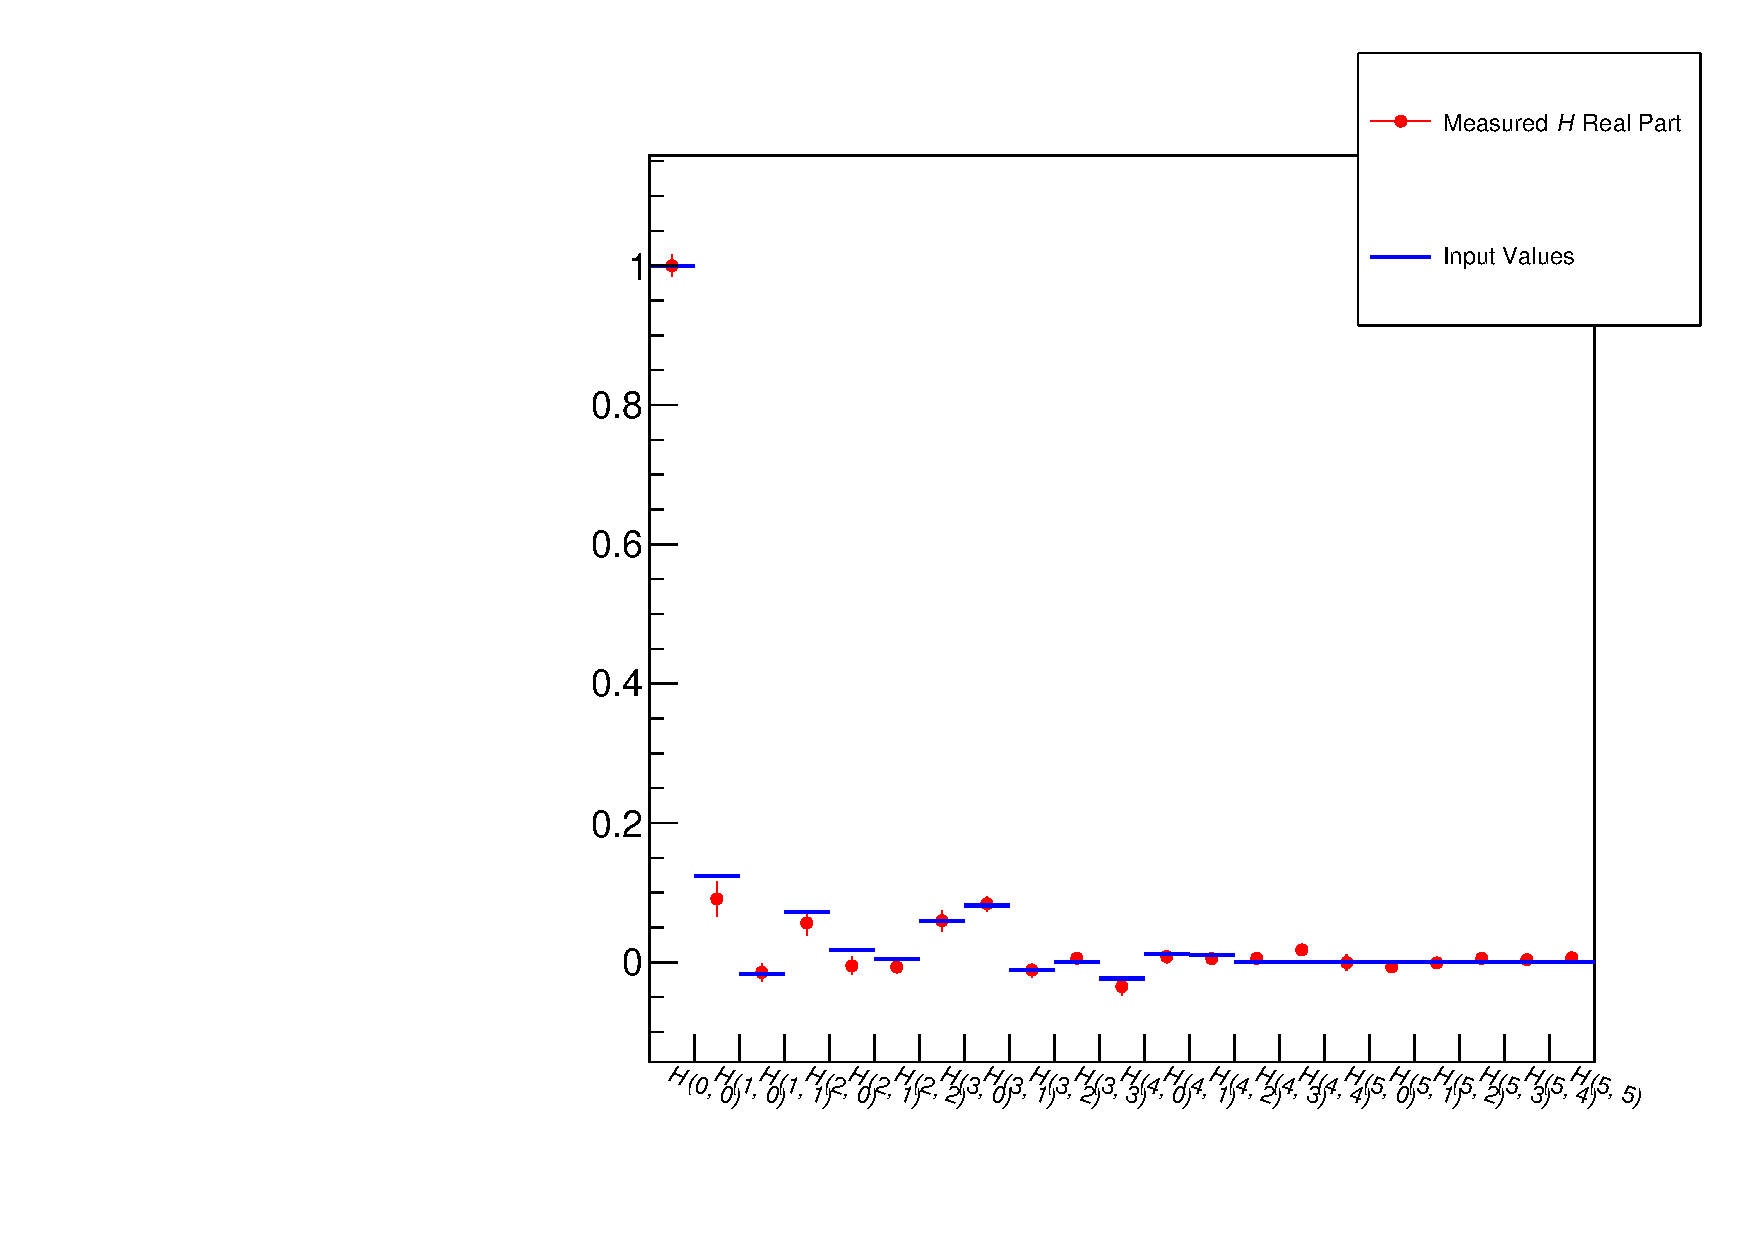
\includegraphics[width=0.5\textwidth]{diffractive/acc_4/hCompare_H_Re}%
  }%
  \subfloat[][]{%
    \label{fig:diffraction_study_comparison_im}%
    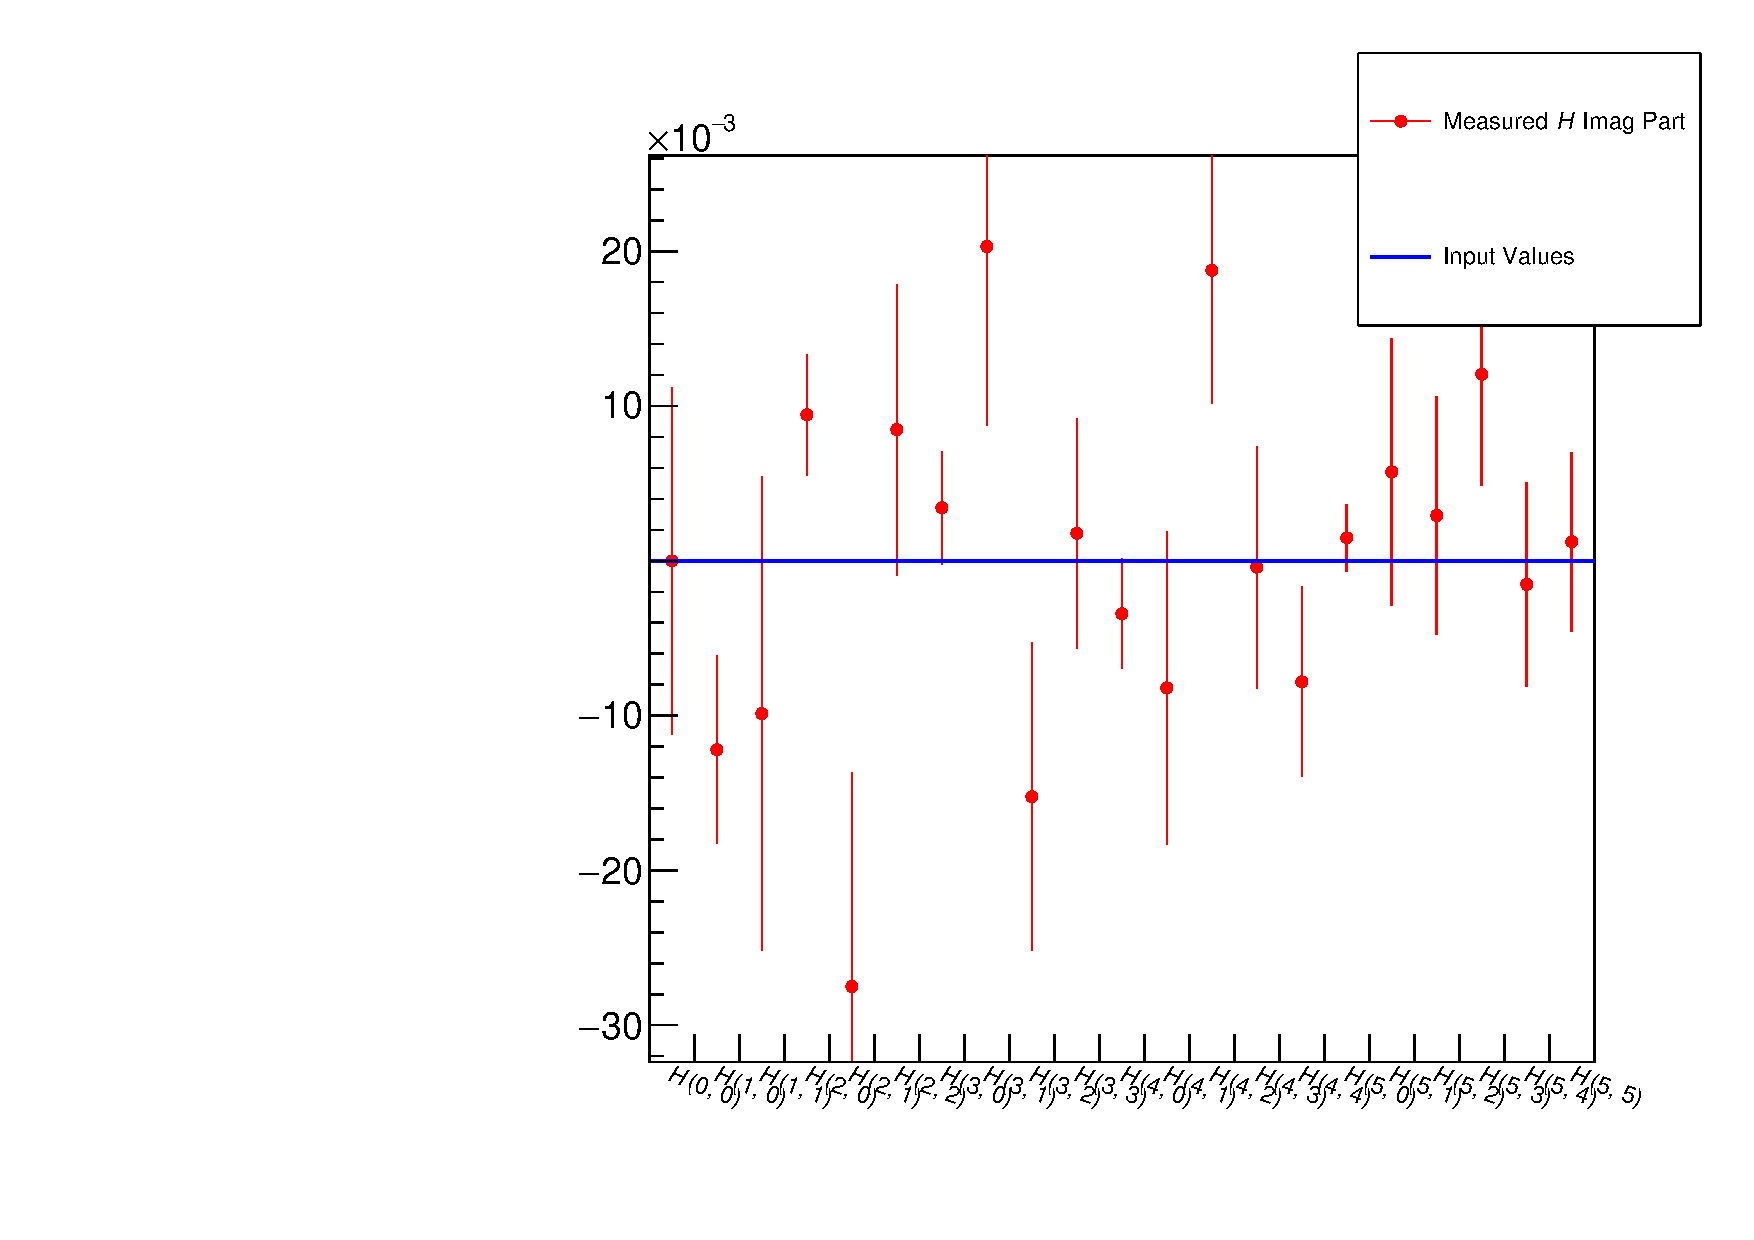
\includegraphics[width=0.5\textwidth]{diffractive/acc_4/hCompare_H_Im}%
  }%
  \\%
  \subfloat[][]{%
    \label{fig:diffraction_study_residual_re}%
    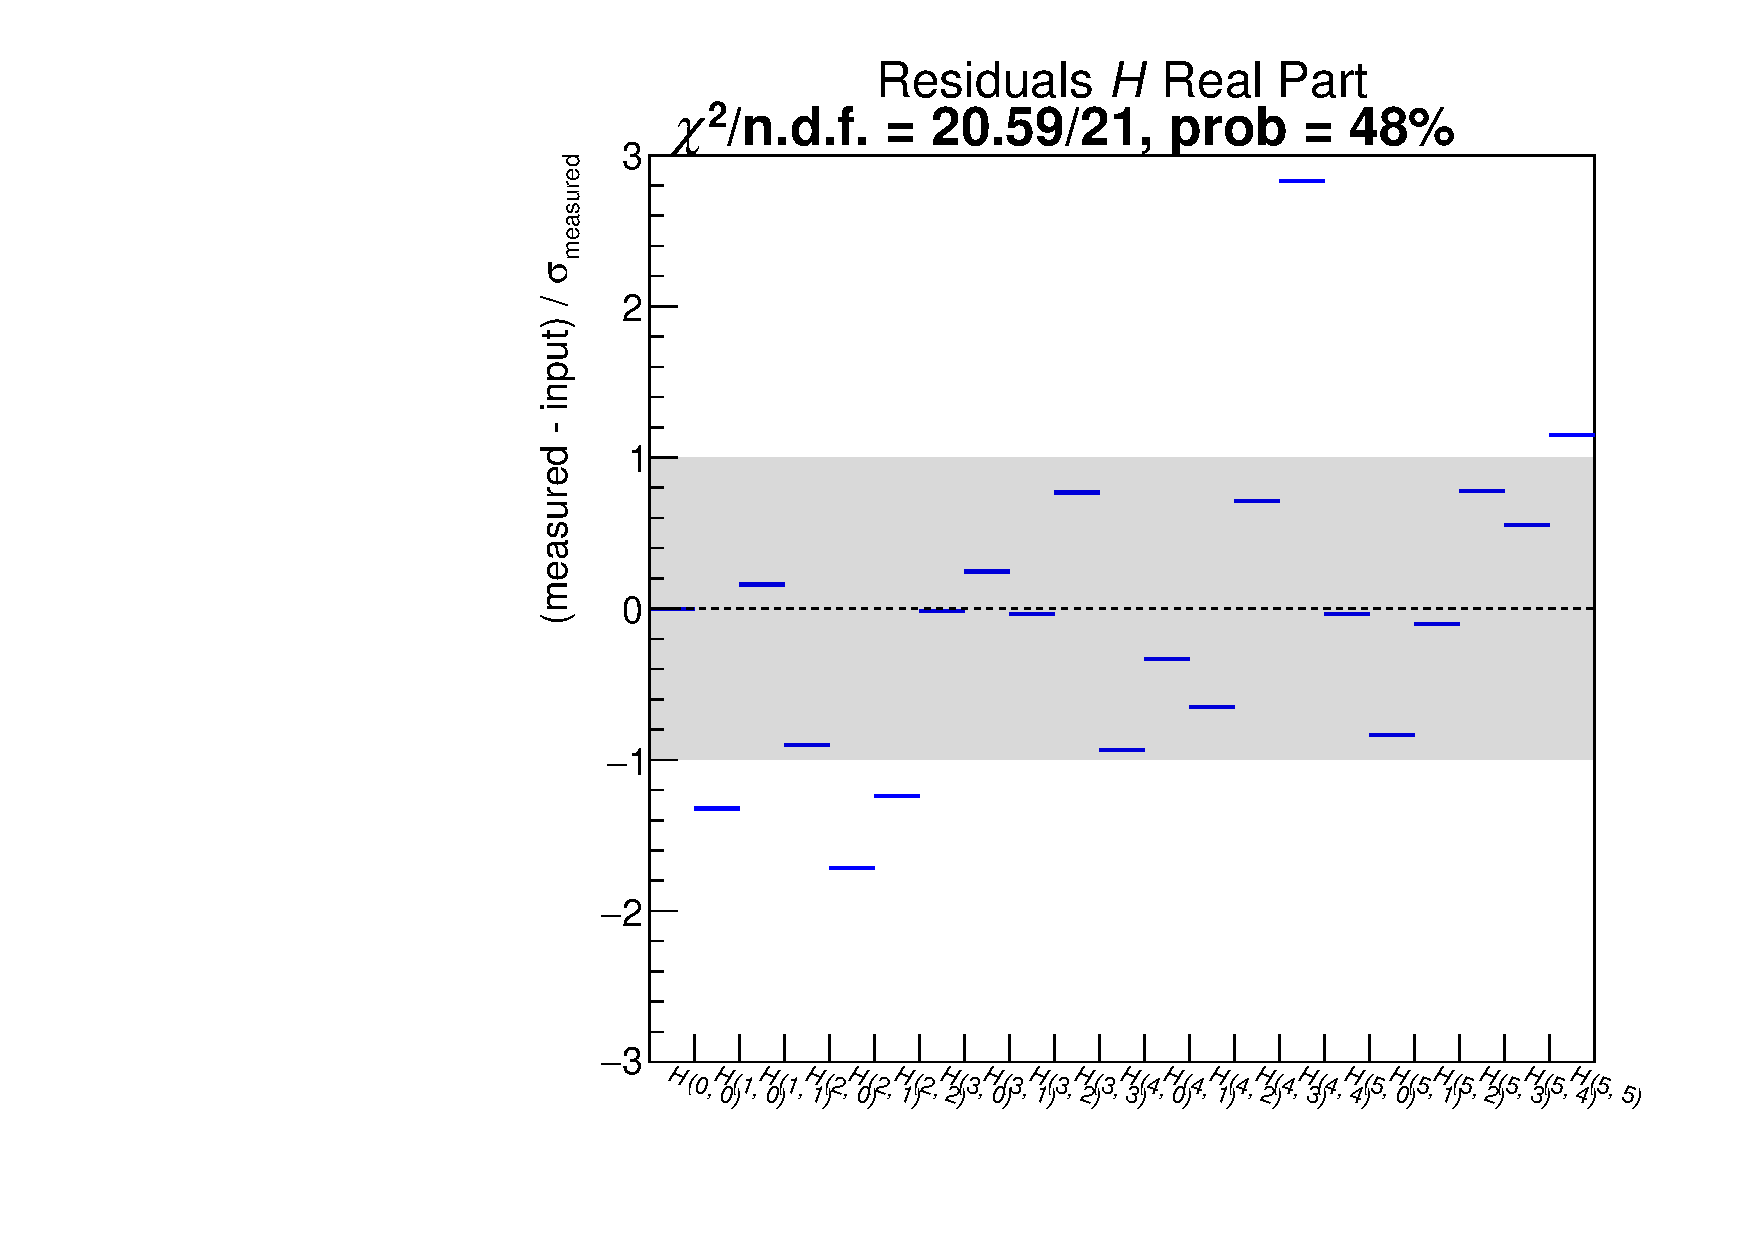
\includegraphics[width=0.5\textwidth]{diffractive/acc_4/hResiduals_H_Re}%
  }%
  \subfloat[][]{%
    \label{fig:diffraction_study_residual_im}%
    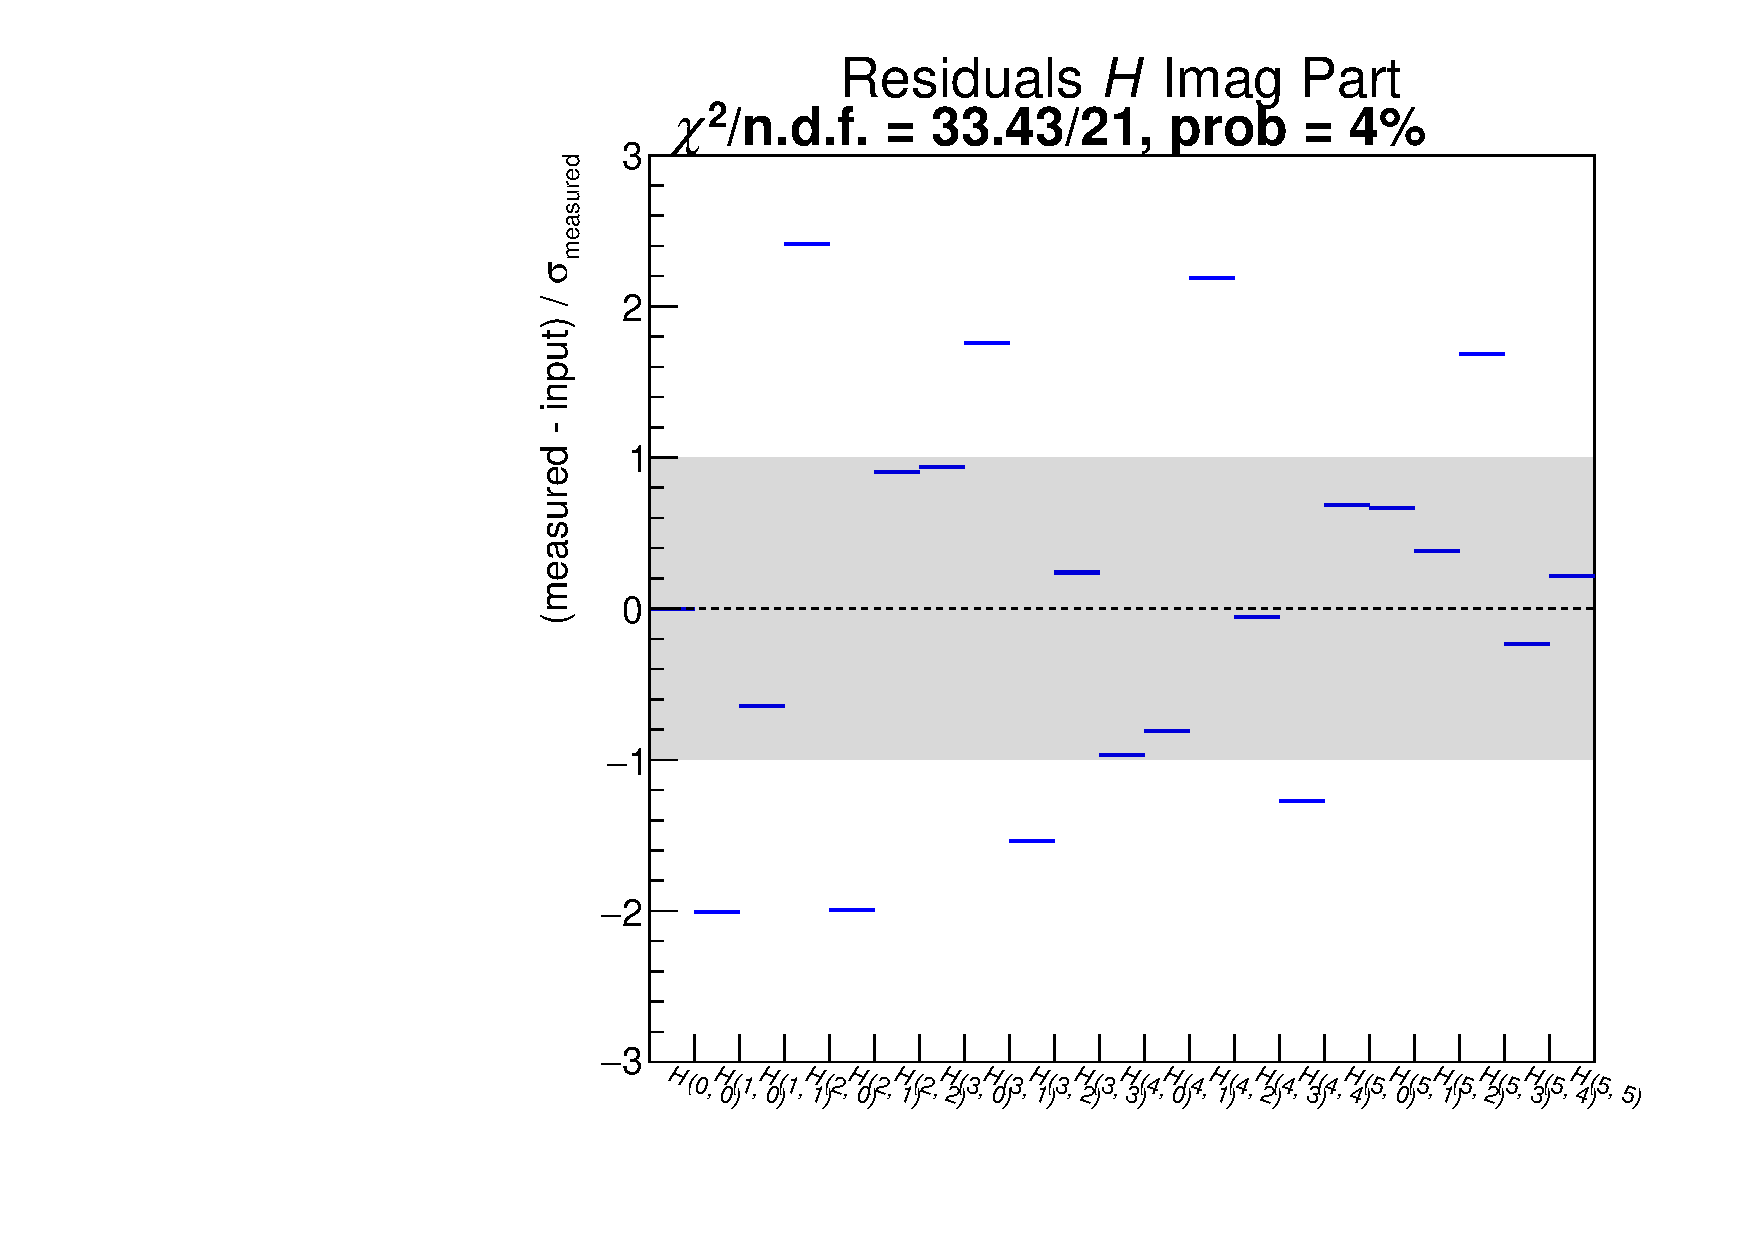
\includegraphics[width=0.5\textwidth]{diffractive/acc_4/hResiduals_H_Im}%
  }%
  \caption{Upper row: Comparison of the physical moments (red points
  with uncertainties) extracted from the Monte Carlo data, which are
  generated using the partial-wave amplitudes in
  \cref{tab:diffraction_study_waveset} and the detection efficiency in
  \cref{eq:diffraction_study_acc1}, with the expected values (blue
  lines).  Both sets of values are normalized to the value of $H_0(0,
  0)$ in the set.
  \subfloatLabel{fig:diffraction_study_comparison_re}~shows the real
  part, \subfloatLabel{fig:diffraction_study_comparison_im}~the
  imaginary part.  Note that moments with $M > 2$ and/or $L > 4$ are
  expected to be zero due to the chosen wave set.  Lower row:
  corresponding residuals.}%
  \label{fig:diffraction_study_output}%
\end{figure}

\todoInl{Discuss acceptance correction using moment decomposition of $\eta^{-1}(\Omega)$}

\clearpage
\section{Photoproduction with linearly polarized beam}%
\label{sec:photoprod}

\subsection{Moment decomposition}%
\label{sec:photoprod:moment}

Systems of two distinguishable spinless particles can also be produced
in photo-production reactions using stationary proton targets.  As in
the case of diffractive reactions discussed in \cref{sec:diffraction},
we are interested in the intermediate meson resonances~$X$ that are
produced in these reactions and that decay into the observed
two-(pseudo)scalar system.  A typical example for such a process is
the reaction
\begin{equation}
  \label{eq:etaOrPr_pi_photoprod}
  \gamma\, p \to X^0\, p \to \etaOrPr\pi^0\, p,
\end{equation}
which is shown in \cref{fig:photoprod_etaprimepi}.  How to analyze
these reactions was studied in detail by the JPAC collaboration
in~\refsCite{Mathieu:2019fts,Mathieu:2019gxo}.  We will follow these
references here and will derive some equations.

\begin{figure}[bp]
  \centering%
  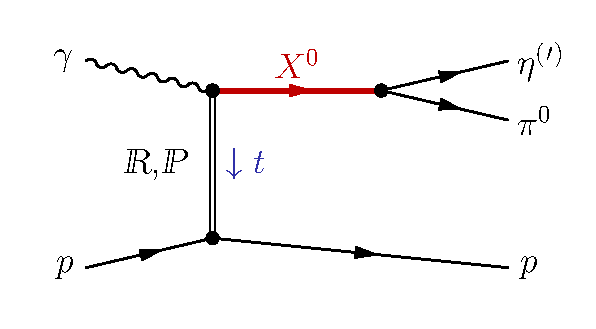
\includegraphics[width=0.5\textwidth]{photoproduction_x_etaprimepi_p}%
  \caption{Scattering of a real photon off a target proton mediated by
  Reggeon exchange.  In this photoproduction process, an intermediate
  state~$X^0$ with well-defined quantum numbers is produced, which in
  the example given here decays into the \etaOrPrPim channel.
  (\Confer~\cref{fig:diffraction_etaprimepi}.)}%
  \label{fig:photoprod_etaprimepi}%
\end{figure}

The analysis is based on the measured intensity distribution, \ie the
number density distribution of events, which is decomposed into
partial-wave amplitudes analogous to the diffractive case in
\cref{eq:diffraction_intensity}:\footnote{\label{fn:photoprod_ampl_redef}This
corresponds to Eq.~(A3) in \refCite{Mathieu:2019fts} with the
phase-space factor~$\kappa$ absorbed into the partial-wave amplitudes,
\ie with the redefinition $\prodAmp \to \prodAmp / \sqrt{\kappa}$ (see
also footnote~6 in \refCite{Mathieu:2019fts}), and with Eq.~(A5)
inserted.}\todo{Can we express this as $\abs{\text{amplitude}}^2$?}
\begin{equation}
  \label{eq:photoprod_intensity}
  \intensity(\Omega, \Phi; w, t)
  = \frac{\dif{N}}{\dif{w}\, \dif{t}\, \dif{\Omega}\, \dif{\Phi}}
  = \sum_{\substack{\ell m \\ \ell' m'}}^\infty
  Y_\ell^m(\Omega)~
  \dUnderbrace{\sum_{\substack{\lambda = \pm 1 \\ \mathclap{\lambda_1, \lambda_2 = \pm 1/2}}}
  \prodAmp^\ell_{\!m\, \lambda; \lambda_1\, \lambda_2}(w, t)\,
  \varrho^\gamma_{\lambda\, \lambda'}(\Phi)\,
  \prodAmp^{\ell' *}_{\!m'\, \lambda'; \lambda_1\, \lambda_2}(w, t)}{\equiv \varrho^{\ell\, \ell'}_{m\, m'}(w, t, \Phi)}~
  Y_{\ell'}^{m' *}(\Omega).
\end{equation}
Here, $N$~is the (acceptance-corrected) number of measured events,
$w$~is the invariant mass of the two-(pseudo)scalar system, $t$~is the
squared four-momentum transferred from the beam to the target
particle, $\Omega = (\theta, \phi)$ is the direction of one of the two
(pseudo)scalar mesons the~$X$ decays into, measured in the
Gottfried-Jackson or helicity rest frame of~$X$, and~$\Phi$ is the
azimuthal angle between the polarization vector of the linearly
polarized photon and the reaction plane in the $X$~rest frame.  The
$\prodAmp^\ell_{\!m\, \lambda; \lambda_1\, \lambda_2}(w, t)$ are
the partial-wave amplitudes that correspond to an intermediate state
with a spin, which is given by the relative orbital angular
momentum~$\ell$ between the two-(pseudo)scalar mesons, and a spin
projection~$m$ \wrt the chosen quantization axis (Gottfried-Jackson
frame: beam direction; helicity frame: momentum direction of~$X$).
This intermediate state is produced in the interaction of a photon
with helicity~$\lambda = \pm 1$ and a target proton with
helicity~$\lambda_1 = \pm 1/2$; the recoil proton has
helicity~$\lambda_2 = \pm 1/2$.  The angular distribution of the
$X$~decay products is given by the spherical harmonics
$Y_\ell^m(\Omega)$~\cite{wikipedia:sphericalHarm} and the dependence
on the polarization angle~$\Phi$ is given by the photon spin-density
matrix~$\mat{\upvarrho}^\gamma(\Phi)$.  In
\cref{eq:photoprod_intensity}, $\varrho^{\ell\, \ell'}_{m\, m'}(w, t,
\Phi)$ is the spin-density matrix element of~$X$ defined analogously
to the diffractive case in \cref{eq:diffraction_spin_dens_def}.

Using the fact that the three Pauli matrices $\vec{\mat{\upsigma}} =
(\mat{\upsigma}_1, \mat{\upsigma}_2, \mat{\upsigma}_3)^T$ and
$\mat{I}_{2 \times 2}$ form a complete set in the space of Hermitian
$2 \times 2$ matrices, we can expand $\mat{\upvarrho}^\gamma(\Phi)$,
\ie
\begin{equation}
  \mat{\upvarrho}^\gamma(\Phi)
  = \frac{1}{2}\, \mat{I}_{2 \times 2} + \frac{1}{2}\, \vec{P}_\gamma(\Phi) \cdot \vec{\mat{\upsigma}}.
\end{equation}
Here, the vector $\vec{P}_\gamma(\Phi)$ describes the photon
polarization.  Its length~$0 \leq P_\gamma \leq 1$ is the degree of
polarization and its direction depends on the kind of
polarization:\footnote{See Eq.~(19) in \refCite{Schilling:1969um}.}
\begin{equation}
  \vec{P}_\gamma(\Phi)
  = \begin{cases*}
    P_\gamma\, (0, 0, \lambda)^T                & for circularly polarized photons with $\lambda = \pm 1$, \\
    -P_\gamma\, (\cos(2 \Phi), \sin(2 \Phi), 0)^T & for linearly polarized photons with polarization angle~$\Phi$.
  \end{cases*}
\end{equation}
Hence, for linearly polarized photons, the intensity distribution in
\cref{eq:photoprod_intensity} can be written as the sum of three
terms:\footnote{See Eq.~(B4) in \refCite{Mathieu:2019fts}.}
\begin{equation}
  \label{eq:photoprod_intensity_sum}
  \intensity(\Omega, \Phi; w, t)
  = \intensity_0(\Omega; w, t)
  - \intensity_1(\Omega; w, t)\, P_\gamma\, \cos(2 \Phi)
  - \intensity_2(\Omega; w, t)\, P_\gamma\, \sin(2 \Phi)
\end{equation}
with the intensity components
\begin{equation}
  \label{eq:photoprod_intensity_components}
  \intensity_i(\Omega; w, t)
  = \sum_{\substack{\ell m \\ \ell' m'}}^\infty
  Y_\ell^m(\Omega)\,
  \prescript{i}{}{\varrho}^{\ell\, \ell'}_{m\, m'}(w, t)\,
  Y_{\ell'}^{m' *}(\Omega);
  \quad i = 0, 1, 2
\end{equation}
and the spin-density matrix components\footnote{See Eq.~(11) in
\refCite{Mathieu:2019fts}.}
\begin{align}
  \label{eq:photoprod_rho_0}
  \prescript{0}{}{\varrho}^{\ell\, \ell'}_{m\, m'}(w, t)
  ={}& \frac{1}{2}\quad \sum_{\substack{\lambda = \pm 1 \\ \mathclap{\lambda_1, \lambda_2 = \pm 1/2}}}
  \prodAmp^\ell_{\!m\, \lambda; \lambda_1\, \lambda_2}(w, t)\,
  \prodAmp^{\ell' *}_{\!m'\, \lambda; \lambda_1\, \lambda_2}(w, t)
  \\
  \label{eq:photoprod_rho_1}
  \prescript{1}{}{\varrho}^{\ell\, \ell'}_{m\, m'}(w, t)
  ={}& \frac{1}{2}\quad \sum_{\substack{\lambda = \pm 1 \\ \mathclap{\lambda_1, \lambda_2 = \pm 1/2}}}
  \prodAmp^\ell_{\!m\, {-\lambda}; \lambda_1\, \lambda_2}(w, t)\,
  \prodAmp^{\ell' *}_{\!m'\, \lambda; \lambda_1\, \lambda_2}(w, t)
  \\
  \label{eq:photoprod_rho_2}
  \prescript{2}{}{\varrho}^{\ell\, \ell'}_{m\, m'}(w, t)
  ={}& \frac{\imag}{2}\quad \sum_{\substack{\lambda = \pm 1 \\ \mathclap{\lambda_1, \lambda_2 = \pm 1/2}}}
  \lambda\,
  \prodAmp^\ell_{\!m\, {-\lambda}; \lambda_1\, \lambda_2}(w, t)\,
  \prodAmp^{\ell' *}_{\!m'\, \lambda; \lambda_1\, \lambda_2}(w, t).
\end{align}
Using the above, the spin-density matrix elements of~$X$ in
\cref{eq:photoprod_intensity} are given by
\begin{equation}
  \label{eq:photoprod_spin_dens_sum}
  \varrho^{\ell\, \ell'}_{m\, m'}(w, t, \Phi)
  = \prescript{0}{}{\varrho}^{\ell\, \ell'}_{m\, m'}(w, t)
  - \prescript{1}{}{\varrho}^{\ell\, \ell'}_{m\, m'}(w, t)\, P_\gamma\, \cos(2 \Phi)
  - \prescript{2}{}{\varrho}^{\ell\, \ell'}_{m\, m'}(w, t)\, P_\gamma\, \sin(2 \Phi).
\end{equation}

Note that in \cref{eq:photoprod_intensity_sum}, the $\Phi$~dependence
is separated, \ie neither the $\intensity_i$ nor the
$\prescript{i}{}{\varrho}^{\ell\, \ell'}_{m\, m'}$ depend on~$\Phi$.
The three intensity components $\intensity_i(\Omega; w, t)$ (as well
as the three spin-density matrix components in
\cref{eq:photoprod_spin_dens_sum}) are modulated by different
$\Phi$~dependences.  From \cref{eq:photoprod_intensity_sum} follows
that
\begin{equation}
  \label{eq:photoprod_unpolarized_intensity}
  \int_{-\pi}^{+\pi}\hspace{-1.2em} \dif{\Phi}\, \intensity(\Omega, \Phi; w, t)
  = 2 \pi\, \intensity_0(\Omega; w, t).
\end{equation}
This means that $I_0(\Omega; w, t)$~corresponds---up to a factor of $2
\pi$---to the unpolarized intensity distribution and is equivalent to
the intensity for the diffractive case in
\cref{eq:diffraction_intensity}.  The other two components
$\intensity_{1, 2}(\Omega; w, t)$ represent additional information
that is accessible in photoproduction with linearly polarized beam.
They depend on the photon polarization and are hence modulated by
different $\Phi$~dependences.  Note that the functions
$\cBrk[1]{f_0(\Phi), f_1(\Phi), f_2(\Phi)} = \cBrk[1]{1, \cos(2 \Phi),
\sin(2 \Phi)}$ that modulate the intensity components constitute an
orthogonal set of functions, \ie
\begin{equation}
  \label{eq:photoprod_orthogonality_phi}
  \int_{-\pi}^{+\pi}\hspace{-1.2em} \dif{\Phi}\, f_i(\Phi)\, f_j(\Phi)
  = (1 + \delta_{i 0})\, \pi\, \delta_{i j};
  \quad i, j = 0 ,1, 2.
\end{equation}

Like for the diffractive case, the partial-wave analysis as well as
the moment decomposition are performed in narrow kinematic cells in
the $(w, t)$ plane, assuming that within each cell all quantities are
in good approximation independent of~$w$ and~$t$.  To simplify
notation we hence omit the~$w$ and $t$~dependencies in all formulas
below, \ie the given formulas are valid in a $(w, t)$ cell.

Analogously to the diffractive case in
\cref{eq:diffraction_intensity_moments}, we decompose the intensity in
\cref{eq:photoprod_intensity_sum} into spherical harmonics to obtain
the moments.  Due to the orthogonality of the $\intensity_i$ terms in
$\Phi$~space, we can decompose each intensity component
separately:\footnote{See Eq.~(A8) in \refCite{Mathieu:2019fts}.}
\begin{align}
  \label{eq:photoprod_intensity_moments_norm_unpol}
  \intensity_0(\Omega)
  ={}& \sum_{L M}^\infty \sqrt{\frac{2 L + 1}{4 \pi}}\, H_0(L, M)\, Y_L^M(\Omega)
  \\
  \label{eq:photoprod_intensity_moments_norm_pol}
  \intensity_{1, 2}(\Omega)
  ={}& -\sum_{L M}^\infty \sqrt{\frac{2 L + 1}{4 \pi}}\, H_{1, 2}(L, M)\, Y_L^M(\Omega).
\end{align}
Here, we have used the same normalization as in
\cref{sec:diffraction:moments_norm}.
\Cref{eq:photoprod_intensity_moments_norm_unpol} is equivalent to
\cref{eq:diffraction_intensity_moments_norm}.  The minus sign in
\cref{eq:photoprod_intensity_moments_norm_pol} is introduced in order
to compensate that the respective intensity components contribute
negatively to the intensity distribution in
\cref{eq:photoprod_intensity_sum}.\footnote{\label{fn:photoprod_intensity_sign}The
minus sign also ensures that $H_1(0, 0) \geq 0$ if the wave set
contains only positive-reflectivity waves with $m \geq 0$ (see
\cref{sec:photoprod:reflectivity} and Appendix~D in
\refCite{Mathieu:2019fts}).}

The corresponding moments are
\begin{align}
  \label{eq:photoprod_moment_norm_unpol}
  H_0(L, M)
  ={}& \frac{1}{2 \pi}\, \sqrt{\frac{4 \pi}{2 L + 1}} \int_{4 \pi}\!\!\!\! \dif{\Omega} \int_{-\pi}^{+\pi}\hspace{-1.2em} \dif{\Phi}\,
  \intensity(\Omega, \Phi)\, Y_L^{M *}(\Omega)
  \\
  \label{eq:photoprod_moments_norm_pol}
  H_{1, 2}(L, M)
  ={}& \frac{1}{\pi P_\gamma}\, \sqrt{\frac{4 \pi}{2 L + 1}} \int_{4 \pi}\!\!\!\! \dif{\Omega} \int_{-\pi}^{+\pi}\hspace{-1.2em} \dif{\Phi}\,
  \intensity(\Omega, \Phi)\, Y_L^{M *}(\Omega) \times \begin{cases*}
    \cos(2 \Phi) & for $i = 1$, \\
    \sin(2 \Phi) & for $i = 2$.
  \end{cases*}
\end{align}
Here, $H_0(L, M)$ is equivalent to \cref{eq:diffraction_moments_norm}
for the diffractive case.\footnote{The $1 / (2 \pi)$ factor comes from
\cref{eq:photoprod_unpolarized_intensity}.}  The two polarized moments
$H_{1, 2}(L, M)$ represent orthogonal angular distributions in~$\Phi$
(see \cref{eq:photoprod_orthogonality_phi}).


\subsection{Relation between moments and partial-wave amplitudes}%
\label{sec:photoprod:moments_pw}

As in the diffractive case (\confer\
\cref{eq:diffraction_moments_pw_norm}), the moments are linear
combinations of the elements of the respective components of the
spin-density matrix of~$X$.  We see this by inserting
\cref{eq:spherical_harm_prod} into
\cref{eq:photoprod_intensity_components} and comparing with
\cref{eq:photoprod_intensity_moments_norm_unpol,eq:photoprod_intensity_moments_norm_pol},
\ie\footnote{See Eq.~(A9) in \refCite{Mathieu:2019fts}.}
\begin{align}
  \label{eq:photoprod_moment_unpol_pw}
  H_0(L, M)
  ={}& \sum_{\substack{\ell m \\ \ell' m'}}^\infty \sqrt{\frac{2 \ell' + 1}{2 \ell + 1}}
  \clebsch{\ell'}{0}{L}{0}{\ell}{0}\, \clebsch{\ell'}{m'}{L}{M}{\ell}{m}\,
  \prescript{0}{}{\varrho}^{\ell\, \ell'}_{m\, m'}
  \\
  \label{eq:photoprod_moments_pol_pw}
  H_{1, 2}(L, M)
  ={}& -\sum_{\substack{\ell m \\ \ell' m'}}^\infty \sqrt{\frac{2 \ell' + 1}{2 \ell + 1}}
  \clebsch{\ell'}{0}{L}{0}{\ell}{0}\, \clebsch{\ell'}{m'}{L}{M}{\ell}{m}\,
  \prescript{1, 2}{}{\varrho}^{\ell\, \ell'}_{m\, m'},
\end{align}
where the $\prescript{i}{}{\varrho}^{\ell\, \ell'}_{m\, m'}$ are given
by \crefrange{eq:photoprod_rho_0}{eq:photoprod_rho_2}.  For given~$(L,
M)$, the Clebsch-Gordan coefficients restrict the sums to those
quantum-number combinations, for which $\ell' + L + \ell =
\text{even}$ (see \cref{eq:ang_mom_sum}), $\abs{\ell' - L} \leq \ell
\leq \ell' + L$, and $m = m' + M$.  This means that if the
partial-wave amplitudes vanish for $\ell, \ell' > \ell_\text{max}$ the
moments~$H_i(L, M)$ will vanish $L > 2 \ell_\text{max}$.


\subsection{Symmetry properties of moments}%
\label{sec:photo_prod:moments_sym}

To derive the symmetry relations for the photoproduction moments we
use the same approach as in \cref{sec:diffraction:moments_sym}.

From the symmetry property of the spherical harmonics in
\cref{eq:spherical_harm_sym} and the definition of the moments in
\cref{eq:photoprod_moment_norm_unpol,eq:photoprod_moments_norm_pol},
we get
\begin{align}
  H_0^*(L, M)
  ={}& (-1)^M\, \frac{1}{2 \pi}\, \sqrt{\frac{4 \pi}{2 L + 1}} \int_{4 \pi}\!\!\!\! \dif{\Omega} \int_{-\pi}^{+\pi}\hspace{-1.2em} \dif{\Phi}\,
  \intensity(\Omega, \Phi)\, Y_L^{(-M) *}(\Omega) \nonumber
  \\
  ={}& (-1)^M\, H_0(L, {-M})
  \\
  H_{1, 2}^*(L, M)
  ={}& (-1)^M\, \frac{1}{\pi P_\gamma}\, \sqrt{\frac{4 \pi}{2 L + 1}} \int_{4 \pi}\!\!\!\! \dif{\Omega} \int_{-\pi}^{+\pi}\hspace{-1.2em} \dif{\Phi}\,
  \intensity(\Omega, \Phi)\, Y_L^{(-M) *}(\Omega) \times \begin{cases*}
    \cos(2 \Phi) & for $i = 1$, \\
    \sin(2 \Phi) & for $i = 2$
  \end{cases*}
  \nonumber
  \\
  ={}& (-1)^M\, H_{1,2}(L, {-M}),
  \intertext{\ie}
  \label{eq:photoprod_moments_sym_1}
  H_i^*(L, M)
  ={}& (-1)^M\, H_i(L, {-M});
  \quad i = 0, 1, 2,
\end{align}
which is analogous to \cref{eq:diffraction_moment_sym_1}.

Since the formulas for the intensity components in
\cref{eq:photoprod_intensity_moments_norm_unpol,eq:photoprod_intensity_moments_norm_pol}
have---up to overall signs---the same form as
\cref{eq:diffraction_intensity_moments_norm} for the diffractive case,
we can use the same arguments that lead us to
\cref{eq:diffraction_intensity_moments_general}.  Thus, all intensity
components are real-valued and only moments with $M \geq 0$ are
required to calculate them, \ie
\begin{align}
  \label{eq:photoprod_intensity_moments_unpol_general}
  \intensity_0(\Omega)
  ={}& \sum_{L = 0}^\infty \sqrt{\frac{2 L + 1}{4 \pi}} \sum_{M = 0}^{L} (2 - \delta_{M 0})\, \Re{H_0(L, M)\, Y_L^M(\Omega)}
  \\
  \label{eq:photoprod_intensity_moments_pol_general}
  \intensity_{1, 2}(\Omega)
  ={}& -\sum_{L = 0}^\infty \sqrt{\frac{2 L + 1}{4 \pi}} \sum_{M = 0}^{L} (2 - \delta_{M 0})\, \Re{H_{1, 2}(L, M)\, Y_L^M(\Omega)}.
\end{align}

Parity conservation and the assumption that $X$~decays into two
daughter particles with identical parity lead to the following
relations for the spin-density matrix components in
\crefrange{eq:photoprod_rho_0}{eq:photoprod_rho_2}:\footnote{See
Eq.~(A15) in \refCite{Mathieu:2019fts}.}
\begin{equation}
  \label{eq:photoprod_spin_dens_parity}
  \prescript{0, 1}{}{\varrho}^{\ell\, \ell'}_{m\, m'}
  = (-1)^{m - m'}\, \varrho^{\ell'\, \ell}_{{-m}\, {-m'}}
  \quad\text{and}\quad
  \prescript{2}{}{\varrho}^{\ell\, \ell'}_{m\, m'}
  = -(-1)^{m - m'}\, \varrho^{\ell'\, \ell}_{{-m}\, {-m'}}.
\end{equation}
The first equations is analogous to
\cref{eq:diffraction_spin_dens_parity}

Using this together with
\cref{eq:photoprod_moment_unpol_pw,eq:photoprod_moments_pol_pw} and the
symmetry property of the Clebsch-Gordan coefficients in
\cref{eq:clebsch_sym2}, we get\footnote{See Eq.~(A16) in
\refCite{Mathieu:2019fts}.}
\begin{align}
  H_{0, 1}(L, -M)
  ={}& \sum_{\substack{\ell m \\ \ell' m'}}^\infty
  \sqrt{\frac{2 \ell' + 1}{2 \ell + 1}}\,
  \clebsch{\ell'}{0}{L}{0}{\ell}{0}\, \clebsch{\ell'}{-m'}{L}{M}{\ell}{-m}\,
  (-1)^{m - m'}\, \prescript{0, 1}{}{\varrho}^{\ell\, \ell'}_{{-m}\, {-m}'} \nonumber
  \\
  \label{eq:photoprod_moments_01_sym_2}
  \equalUsing{$\mathclap{\substack{\displaystyle{m \to -m} \\ \displaystyle{m' \to -m'}}}$}{}& \quad
  (-1)^M\, H_{0, 1}(L, M)
  \\
  H_2(L, -M)
  ={}& -\sum_{\substack{\ell m \\ \ell' m'}}^\infty
  \sqrt{\frac{2 \ell' + 1}{2 \ell + 1}}\,
  \clebsch{\ell'}{0}{L}{0}{\ell}{0}\, \clebsch{\ell'}{-m'}{L}{M}{\ell}{-m}\,
  (-1)^{m - m'}\, \prescript{2}{}{\varrho}^{\ell\, \ell'}_{{-m}\, {-m}'} \nonumber
  \\
  \label{eq:photoprod_moment_2_sym_2}
  \equalUsing{$\mathclap{\substack{\displaystyle{m \to -m} \\ \displaystyle{m' \to -m'}}}$}{}& \quad
  -(-1)^M\, H_2(L, M).
\end{align}
In the last steps of each equation, we used that the second
Clebsch-Gordan coefficient enforces $m' - M = m$,\footnote{Therefore,
$(-1)^{m - m'} = (-1)^{m' - m} = (-1)^M$.} rearranged the terms in the
sum, and compared to
\cref{eq:photoprod_moment_unpol_pw,eq:photoprod_moments_pol_pw}.

From
\cref{eq:photoprod_moments_sym_1,eq:photoprod_moments_01_sym_2,eq:photoprod_moment_2_sym_2}
it follows that
\begin{equation}
  \label{eq:photoprodP_moments_real_imag}
  H_{0, 1}^*(L, M)
  = H_{0, 1}(L, M)
  \quad\text{and}\quad
  H_2^*(L, M)
  = -H_2(L, M).
\end{equation}
Hence, all $H_{0, 1}(L, M)$ must be real-valued and all $H_2(L, M)$
must be purely imaginary.  Consequently, from
\cref{eq:photoprod_moment_norm_unpol,eq:photoprod_moments_norm_pol},
we get\footnote{See Eq.~(B6) in \refCite{Mathieu:2019fts}.}
\begin{align}
  \label{eq:photoprod_moment_0_real}
  H(L, M)
  ={}& \frac{1}{2 \pi}\, \sqrt{\frac{4 \pi}{2 L + 1}} \int_{4 \pi}\!\!\!\! \dif{\Omega} \int_{-\pi}^{+\pi}\hspace{-1.2em} \dif{\Phi}\,
  \intensity(\Omega, \Phi)\, y_L^M(\theta)\, \cos(M\, \phi)
  \\
  \label{eq:photoprod_moment_0_imag}
  0
  ={}& \frac{1}{2 \pi}\, \sqrt{\frac{4 \pi}{2 L + 1}} \int_{4 \pi}\!\!\!\! \dif{\Omega} \int_{-\pi}^{+\pi}\hspace{-1.2em} \dif{\Phi}\,
  \intensity(\Omega, \Phi)\, y_L^M(\theta)\, \sin(M\, \phi)
  \\
  \label{eq:photoprod_moment_1_real}
  H_1(L, M)
  ={}& \frac{1}{\pi P_\gamma}\, \sqrt{\frac{4 \pi}{2 L + 1}} \int_{4 \pi}\!\!\!\! \dif{\Omega} \int_{-\pi}^{+\pi}\hspace{-1.2em} \dif{\Phi}\,
  \intensity(\Omega, \Phi)\, y_L^M(\theta)\, \cos(M\, \phi)\, \cos(2 \Phi)
  \\
  \label{eq:photoprod_moment_1_imag}
  0
  ={}& \frac{1}{\pi P_\gamma}\, \sqrt{\frac{4 \pi}{2 L + 1}} \int_{4 \pi}\!\!\!\! \dif{\Omega} \int_{-\pi}^{+\pi}\hspace{-1.2em} \dif{\Phi}\,
  \intensity(\Omega, \Phi)\, y_L^M(\theta)\, \sin(M\, \phi)\, \cos(2 \Phi)
  \\
  \label{eq:photoprod_moment_2_real}
  0
  ={}& \frac{1}{\pi P_\gamma}\, \sqrt{\frac{4 \pi}{2 L + 1}} \int_{4 \pi}\!\!\!\! \dif{\Omega} \int_{-\pi}^{+\pi}\hspace{-1.2em} \dif{\Phi}\,
  \intensity(\Omega, \Phi)\, y_L^M(\theta)\, \cos(M\, \phi)\, \sin(2 \Phi)
  \\
  \label{eq:photoprod_moment_2_imag}
  H_2(L, M)
  ={}& -\imag \frac{1}{\pi P_\gamma}\, \sqrt{\frac{4 \pi}{2 L + 1}} \int_{4 \pi}\!\!\!\! \dif{\Omega} \int_{-\pi}^{+\pi}\hspace{-1.2em} \dif{\Phi}\,
  \intensity(\Omega, \Phi)\, y_L^M(\theta)\, \sin(M\, \phi)\, \sin(2 \Phi)
\end{align}
The first two equations are equivalent to
\cref{eq:diffraction_moments_real,eq:diffraction_moments_imag}.  Note
that since $\sin(M\, \phi) = 0$ for $M = 0$,
\begin{equation}
  \label{eq:photoprod_moment_2_M0}
  H_2(L, 0) = 0
  \quad\forall\; L.
\end{equation}

Analogous to \cref{eq:diffraction_intensity_moments_real} for the
diffractive case, we can rewrite
\cref{,eq:photoprod_intensity_moments_unpol_general,eq:photoprod_intensity_moments_pol_general}
taking into account
\cref{eq:photoprodP_moments_real_imag}:\footnote{See Eq.~(A17) in
\refCite{Mathieu:2019fts}.}
\begin{align}
  \intensity_0(\Omega)
  ={}& \sum_{L = 0}^\infty \sqrt{\frac{2 L + 1}{4 \pi}} \sum_{M = 0}^{L} (2 - \delta_{M 0})\, H_0(L, M)\, \Re{Y_L^M(\Omega)} \nonumber
  \\
  \label{eq:photoprod_intensity_0_moments_real}
  ={}& \sum_{L = 0}^\infty \sqrt{\frac{2 L + 1}{4 \pi}} \sum_{M = 0}^{L} (2 - \delta_{M 0})\, H_0(L, M)\, y_L^M(\theta)\, \cos(M\, \phi)
  \\
  \intensity_1(\Omega)
  ={}& -\sum_{L = 0}^\infty \sqrt{\frac{2 L + 1}{4 \pi}} \sum_{M = 0}^{L} (2 - \delta_{M 0})\, H_1(L, M)\, \Re{Y_L^M(\Omega)} \nonumber
  \\
  \label{eq:photoprod_intensity_1_moments_real}
  ={}& -\sum_{L = 0}^\infty \sqrt{\frac{2 L + 1}{4 \pi}} \sum_{M = 0}^{L} (2 - \delta_{M 0})\, H_1(L, M)\, y_L^M(\theta)\, \cos(M\, \phi)
  \\
  \intensity_2(\Omega)
  ={}& \sum_{L = 0}^\infty \sqrt{\frac{2 L + 1}{4 \pi}} \sum_{M = 0}^{L} (2 - \delta_{M 0})\, \Im{H_2(L, M)}\, \Im{Y_L^M(\Omega)} \nonumber
  \\
  \label{eq:photoprod_intensity_2_moments_imag}
  ={}& -\imag \sum_{L = 0}^\infty \sqrt{\frac{2 L + 1}{4 \pi}} \sum_{M = 0}^{L} (2 - \delta_{M 0})\, H_2(L, M)\, y_L^M(\theta)\, \sin(M\, \phi).
\end{align}
Note that \cref{eq:photoprod_intensity_2_moments_imag} is identical to
the corresponding expression in Eq.~(A17) in
\refCite{Mathieu:2019fts}, if one considers that $H_2(L, 0) = 0$
(including the corresponding $M = 0$ terms into the sum hence leaves
its value unchanged) and that $\Im{H_2(L, M)} = -\imag H_2(L, M)$
because $H_2(L, M)$ is purely imaginary (see
\cref{eq:photoprod_moment_2_imag}).  Compared to
\refCite{Mathieu:2019fts}, our formulation is more symmetrical \wrt
\cref{eq:photoprod_intensity_0_moments_real,eq:photoprod_intensity_1_moments_real}.

Since $H_{0, 1}(L, M)$ is real-valued and $H_2(L, M)$ purely
imaginary, it is clear from
\crefrange{eq:photoprod_intensity_0_moments_real}{eq:photoprod_intensity_2_moments_imag}
that the $\intensity_i(\Omega)$ are all real-valued, as expected.
Also note that $\intensity_{0, 1}(\Omega)$ are even functions
in~$\phi$, whereas $\intensity_2(\Omega)$ is an odd function
in~$\phi$.


\subsection{Reflectivity basis}%
\label{sec:photoprod:reflectivity}

In Appendix~D of \refCite{Mathieu:2019fts}, the reflectivity basis is
introduced by defining the partial-wave amplitudes\footnote{See
Eq.~(D1) in \refCite{Mathieu:2019fts}.}\footnote{Alternative
approaches to apply the reflectivity basis are discussed in
\refCite{Salgado:2020}.}
\begin{equation}
  \label{eq:photoprod_amplitude_refl}
  \prescript{\refl}{}{\prodAmp}^\ell_{\!m; \lambda_1\, \lambda_2}
  \equiv \frac{1}{2}\, \sBrk{\prodAmp^\ell_{\!m\, {+1}; \lambda_1\, \lambda_2}
  - \refl\, (-1)^m\, \prodAmp^\ell_{\!{-m}\, {-1}; \lambda_1\, \lambda_2}},
\end{equation}
which are linear combinations of partial-wave amplitudes with opposite
photon helicities~$\lambda$ and opposite $X$~spin projection quantum
numbers~$m$, where $m = -\ell, \ldots, +\ell$.  Hence, the
reflectivity quantum number $\refl = \pm$ effectively replaces the
photon helicity $\lambda = \pm 1$ such that the total number of
amplitudes for given~$\ell$ and~$m$ remains unchanged.

Formulating the intensity model in the reflectivity basis has the
advantage that in the high-energy limit at leading order,
\refl~corresponds to the naturality of the spin-parity exchanged in
the scattering process (see Appendices~C and~D in
\refCite{Mathieu:2019fts}).  Another advantage of the reflectivity
basis is that due to parity conservation partial-wave amplitudes with
opposite~\refl do not interfere.\footnote{See Eq.~(D5) in
\refCite{Mathieu:2019fts}.}  Parity conservation also directly relates
partial-wave amplitudes with opposite helicities of the target and the
recoil proton, \ie\footnote{See Eq.~(D3) in
\refCite{Mathieu:2019fts}.}
\begin{equation}
  \label{eq:photoprod_amplitude_parity_refl}
  \prescript{\refl}{}{\prodAmp}^\ell_{\!m; {-\lambda_1}\, {-\lambda_2}}
  = \refl\, (-1)^{\lambda_1 - \lambda_2}\, \prescript{\refl}{}{\prodAmp}^\ell_{\!m; \lambda_1\, \lambda_2}.
\end{equation}
Therefore, for given~\refl, $\ell$, and~$m$, only two of the four
possible partial-wave amplitudes are independent,%
\footnote{In general, scattering reactions with a recoil particle with
spin~$J_R$ are described by $2 J_R + 1$ independent amplitudes
$\sBrk{\ell}^{(\refl)}_{m; k}$ with $k = 0, \ldots, 2 J_R$.}
namely the proton spin-flip amplitude\footnote{See Eq.~(D4) in
\refCite{Mathieu:2019fts}.}
\begin{align}
  \prescript{\refl}{}{\prodAmp}^\ell_{\!m; {+1}\, {-1}}
  \equiv{}& \sBrk{\ell}^{(\refl)}_{m; 0}
  \intertext{and the proton spin-non-flip amplitude}
  \prescript{\refl}{}{\prodAmp}^\ell_{\!m; {+1}\, {+1}}
  \equiv{}& \sBrk{\ell}^{(\refl)}_{m; 1}.
\end{align}
Furthermore, since parity is conserved the spin-flip and
spin-non-flip amplitudes do not interfere. In the conventional basis,
it would be difficult to incorporate these parity constraints into
\crefrange{eq:photoprod_intensity_components}{eq:photoprod_rho_2}
because parity relates those $\prodAmp^\ell_{\!m\, \lambda;
\lambda_1\, \lambda_2}$ that in addition to opposite~$\lambda_1$
and~$\lambda_2$ quantum numbers also have opposite~$m$
and~$\lambda$.\footnote{See Eq.~(A14) in \refCite{Mathieu:2019fts}.}
However, in the reflectivity basis we can simply write\footnote{See
Eq.~(D7) in \refCite{Mathieu:2019fts}.}
\begin{equation}
  \label{eq:photoprod_rho_refl}
  \prescript{i}{}{\varrho}^{\ell\, \ell'}_{m\, m'}
  = \prescript{i}{}{\varrho}^{(+)\, \ell\, \ell'}_{m\, m'} + \prescript{i}{}{\varrho}^{(-)\, \ell\, \ell'}_{m\, m'};
  \quad i = 0, 1, 2
\end{equation}
with\footnote{See Eq.~(D8) in \refCite{Mathieu:2019fts} and
\cref{fn:photoprod_ampl_redef}.}
\begin{align}
  \label{eq:photoprod_rho_0_refl}
  \prescript{0}{}{\varrho}^{(\refl)\, \ell\, \ell'}_{m\, m'}
  ={}& \sum_{k = 0, 1} \rBrk[2]{\sBrk{\ell}^{(\refl)}_{m; k}\, \sBrk{\ell'}^{(\refl) *}_{m'; k}
  + (-1)^{m - m'}\, \sBrk{\ell}^{(\refl)}_{{-m}; k}\, \sBrk{\ell'}^{(\refl) *}_{{-m'}; k}}
  \\
  \label{eq:photoprod_rho_1_refl}
  \prescript{1}{}{\varrho}^{(\refl)\, \ell\, \ell'}_{m\, m'}
  ={}& -\refl \sum_{k = 0, 1}
  \rBrk[2]{(-1)^m\, \sBrk{\ell}^{(\refl)}_{{-m}; k}\, \sBrk{\ell'}^{(\refl) *}_{m'; k}
  + (-1)^{m'}\, \sBrk{\ell}^{(\refl)}_{m; k}\, \sBrk{\ell'}^{(\refl) *}_{{-m'}; k}}
  \\
  \label{eq:photoprod_rho_2_refl}
  \prescript{2}{}{\varrho}^{(\refl)\, \ell\, \ell'}_{m\, m'}
  ={}& -\imag\, \refl \sum_{k = 0, 1}
  \rBrk[2]{(-1)^m\, \sBrk{\ell}^{(\refl)}_{{-m}; k}\, \sBrk{\ell'}^{(\refl) *}_{m'; k}
  - (-1)^{m'}\, \sBrk{\ell}^{(\refl)}_{m; k}\, \sBrk{\ell'}^{(\refl) *}_{{-m'}; k}}.
\end{align}
In \cref{eq:photoprod_rho_refl}, we sum incoherently over~$\refl =
\pm$ and in
\crefrange{eq:photoprod_rho_0_refl}{eq:photoprod_rho_2_refl}, we sum
incoherently over~$k = 0, 1$, \ie the rank of the
$\prescript{i}{}{\varrho}^{(\refl)\, \ell\, \ell'}_{m\, m'}$ is in
general~2.  By inserting \cref{eq:photoprod_rho_refl} into
\cref{eq:photoprod_intensity_components}, we obtain the intensity
components in the reflectivity basis:
\begin{equation}
  \label{eq:photoprod_intensity_components_refl}
  \intensity_i(\Omega)
  = \sum_{\substack{\ell m \\ \ell' m'}}^\infty
  Y_\ell^m(\Omega)
  \sBrk[3]{\, \sum_{\refl = \pm} \prescript{i}{}{\varrho}^{(\refl)\, \ell\, \ell'}_{m\, m'}}
  Y_{\ell'}^{m' *}(\Omega);
  \quad i = 0, 1, 2
\end{equation}

Note that usually neither the spin of the target proton
nor the one of the recoil proton is measured.  Still, the intensity
distribution obtained by inserting
\crefrange{eq:photoprod_rho_refl}{eq:photoprod_rho_2_refl} into
\cref{eq:photoprod_intensity_components} has two incoherent sectors
indexed by~$k = 0, 1$ as required by parity conservation.  However, in
this case $k$~has no direct physical interpretation anymore, \ie
experimentally we cannot distinguish, which value of~$k$ belongs to
proton spin-flip and which to proton spin-non-flip.  In practice, one
often assumes that either the spin-non-flip or the spin-flip
amplitudes dominate and sets $k = 0$.  This means the partial-wave
amplitudes are all fully coherent and the spin-density matrix
components in
\crefrange{eq:photoprod_rho_0_refl}{eq:photoprod_rho_2_refl} have
rank~1.

We can relate the moments to the partial-wave amplitudes in the
reflectivity basis by inserting
\crefrange{eq:photoprod_rho_0_refl}{eq:photoprod_rho_2_refl} into
\cref{eq:photoprod_moment_unpol_pw,eq:photoprod_moments_pol_pw}:
\begin{align}
  \label{eq:photoprod_moment_0_pw_refl}
  H_0(L, M)
  ={}& \begin{multlined}[t][0.8\columnwidth]
    \sum_{\substack{\ell m \\ \ell' m'}}^\infty \sqrt{\frac{2 \ell' + 1}{2 \ell + 1}}
    \clebsch{\ell'}{0}{L}{0}{\ell}{0}\, \clebsch{\ell'}{m'}{L}{M}{\ell}{m} \\[-2ex]
    \shoveleft{\hfill \times%
      \sum_{\refl = \pm} \sum_{k = 0, 1} \rBrk[2]{\sBrk{\ell}^{(\refl)}_{m; k}\, \sBrk{\ell'}^{(\refl) *}_{m'; k}
      + (-1)^{m - m'}\, \sBrk{\ell}^{(\refl)}_{{-m}; k}\, \sBrk{\ell'}^{(\refl) *}_{{-m'}; k}}
    }
  \end{multlined}
  \\
  \label{eq:photoprod_moment_1_pw_refl}
  H_1(L, M)
  ={}& \begin{multlined}[t][0.8\columnwidth]
    \sum_{\substack{\ell m \\ \ell' m'}}^\infty \sqrt{\frac{2 \ell' + 1}{2 \ell + 1}}
    \clebsch{\ell'}{0}{L}{0}{\ell}{0}\, \clebsch{\ell'}{m'}{L}{M}{\ell}{m} \\[-2ex]
    \shoveleft{\hfill \times%
      \sum_{\refl = \pm} \refl \sum_{k = 0, 1} \rBrk[2]{(-1)^m\, \sBrk{\ell}^{(\refl)}_{{-m}; k}\, \sBrk{\ell'}^{(\refl) *}_{m'; k}
      + (-1)^{m'}\, \sBrk{\ell}^{(\refl)}_{m; k}\, \sBrk{\ell'}^{(\refl) *}_{{-m'}; k}}
    }
  \end{multlined}
  \\
  \label{eq:photoprod_moment_2_pw_refl}
  H_2(L, M)
  ={}& \begin{multlined}[t][0.8\columnwidth]
    \imag \sum_{\substack{\ell m \\ \ell' m'}}^\infty \sqrt{\frac{2 \ell' + 1}{2 \ell + 1}}
    \clebsch{\ell'}{0}{L}{0}{\ell}{0}\, \clebsch{\ell'}{m'}{L}{M}{\ell}{m} \\[-2ex]
    \shoveleft{\hfill \times%
      \sum_{\refl = \pm} \refl \sum_{k = 0, 1} \rBrk[2]{(-1)^m\, \sBrk{\ell}^{(\refl)}_{{-m}; k}\, \sBrk{\ell'}^{(\refl) *}_{m'; k}
      - (-1)^{m'}\, \sBrk{\ell}^{(\refl)}_{m; k}\, \sBrk{\ell'}^{(\refl) *}_{{-m'}; k}}
    }.
  \end{multlined}
\end{align}
It is important to note that each moment is an incoherent sum of
contributions from both reflectivities, \ie the moments do not
separate these contributions.  Also note that in
\cref{eq:photoprod_moment_0_pw_refl} the contributions from the two
reflectivities enter with the same sign, whereas in
\cref{eq:photoprod_moment_1_pw_refl,eq:photoprod_moment_2_pw_refl}
they enter with opposite sign.  Similarly, each moment is an
incoherent sum over~$k$, \ie the moments do not separate spin-flip and
spin-non-flip amplitudes.

From
\cref{eq:photoprod_moment_0_real,eq:photoprod_moment_0_pw_refl,eq:photoprod_moment_1_pw_refl,eq:photoprod_moment_2_pw_refl}
it follows that in particular
\begin{align}
  H_0(0, 0)
  = \frac{1}{2 \pi} \int_{4 \pi}\!\!\!\! \dif{\Omega} \int_{-\pi}^{+\pi}\hspace{-1.2em} \dif{\Phi}\,
  \intensity(\Omega, \Phi)
  ={}& \sum_{\ell m}^\infty \prescript{0}{}{\varrho}^{\ell\, \ell}_{m\, m}
  = \sum_{\ell m}^\infty \sum_{\refl = \pm} \sum_{k = 0, 1}
  \rBrk[2]{\Abs[1]{\sBrk{\ell}^{(\refl)}_{m; k}}^2 + \Abs[1]{\sBrk{\ell}^{(\refl)}_{{-m}; k}}^2} \nonumber
  \\
  \label{eq:photoprod_monent_00_refl}
  ={}& 2 \sum_{\ell m}^\infty \sum_{k = 0, 1}
  \rBrk[2]{\Abs[1]{\sBrk{\ell}^{(+)}_{m; k}}^2 + \Abs[1]{\sBrk{\ell}^{(-)}_{m; k}}^2}
  \\
  H_1(0, 0)
  ={}& -\sum_{\ell m}^\infty \prescript{1}{}{\varrho}^{\ell\, \ell}_{m\, m}
  = \sum_{\ell m}^\infty \sum_{\refl = \pm} \refl \sum_{k = 0, 1}
  (-1)^m \rBrk[2]{\sBrk{\ell}^{(\refl)}_{{-m}; k}\, \sBrk{\ell}^{(\refl) *}_{m; k}
  + \sBrk{\ell}^{(\refl)}_{m; k}\, \sBrk{\ell}^{(\refl) *}_{{-m}; k}}
  \\
  H_2(0, 0)
  ={}& -\sum_{\ell m}^\infty \prescript{2}{}{\varrho}^{\ell\, \ell}_{m\, m}
  = \imag \sum_{\ell m}^\infty \sum_{\refl = \pm} \refl \sum_{k = 0, 1}
  (-1)^m \rBrk[2]{\sBrk{\ell}^{(\refl)}_{{-m}; k}\, \sBrk{\ell}^{(\refl) *}_{m; k}
  - \sBrk{\ell}^{(\refl)}_{m; k}\, \sBrk{\ell}^{(\refl) *}_{{-m}; k}}
\end{align}
Like in the diffractive case (\confer\
\cref{eq:diffraction_moment_00_pw,eq:diffraction_moment_00_pw_refl}),
the lowest unpolarized moment $H_0(0, 0)$ is identical to the
intensity integral and the sum of all partial-wave
intensities.\footnote{The factor~2 in the right-hand side of
\cref{eq:photoprod_monent_00_refl} appears because---due to
\cref{eq:photoprod_amplitude_parity_refl}---we replaced four
amplitudes for the various proton helicities by two amplitudes for
proton spin-flip and spin-non-flip.}

We can simplify the equations for $H_1(0, 0)$ and $H_2(0, 0)$ further
by using
\begin{align}
  \sum_{m = -\ell}^{m = +\ell}
  (-1)^m \sBrk{\ell}^{(\refl)}_{m; k}\, \sBrk{\ell}^{(\refl) *}_{{-m}; k}
  ={}& \sum_{m = -\ell}^{m = -1}
  (-1)^m \sBrk{\ell}^{(\refl)}_{m; k}\, \sBrk{\ell}^{(\refl) *}_{{-m}; k}
  + \sBrk{\ell}^{(\refl)}_{0; k}\, \sBrk{\ell}^{(\refl) *}_{0; k}
  + \sum_{m = +1}^{m = +\ell}
  (-1)^m \sBrk{\ell}^{(\refl)}_{m; k}\, \sBrk{\ell}^{(\refl) *}_{{-m}; k} \nonumber
  \\
  ={}& \Abs[2]{\sBrk{\ell}^{(\refl)}_{0; k}}^2
  + \sum_{m = +1}^{m = +\ell}
  (-1)^m \rBrk[2]{\sBrk{\ell}^{(\refl)}_{m; k}\, \sBrk{\ell}^{(\refl) *}_{{-m}; k} + \sBrk{\ell}^{(\refl) *}_{m; k}\, \sBrk{\ell}^{(\refl)}_{{-m}; k}} \nonumber
  \\
  ={}& \Abs[2]{\sBrk{\ell}^{(\refl)}_{0; k}}^2
  + 2 \sum_{m = +1}^{m = +\ell}
  (-1)^m \Re[2]{\sBrk{\ell}^{(\refl)}_{m; k}\, \sBrk{\ell}^{(\refl) *}_{{-m}; k}}
  \in \mathbb{R}.
\end{align}
Using the above, we see that
\begin{align}
  H_1(0, 0)
  ={}& \sum_{\refl = \pm} \refl \sum_{k = 0, 1} \sum_{\ell}^\infty
  \rBrk[3]{\Abs[2]{\sBrk{\ell}^{(\refl)}_{0; k}}^2
  + 2 \sum_{m = +1}^{m = +\ell}
  (-1)^m \Re[2]{\sBrk{\ell}^{(\refl)}_{{-m}; k}\, \sBrk{\ell}^{(\refl) *}_{m; k}}
  + \Abs[2]{\sBrk{\ell}^{(\refl)}_{0; k}}^2
  + 2 \sum_{m = +1}^{m = +\ell}
  (-1)^m \Re[2]{\sBrk{\ell}^{(\refl)}_{m; k}\, \sBrk{\ell}^{(\refl) *}_{{-m}; k}}} \nonumber
  \\
  ={}& 2 \sum_{\refl = \pm} \refl \sum_{k = 0, 1} \sum_{\ell}^\infty
  \rBrk[3]{\Abs[2]{\sBrk{\ell}^{(\refl)}_{0; k}}^2
  + 2 \sum_{m = +1}^{m = +\ell}
  (-1)^m \Re[2]{\sBrk{\ell}^{(\refl)}_{{-m}; k}\, \sBrk{\ell}^{(\refl) *}_{m; k}}}
  \\
  H_2(0, 0)
  ={}& \imag \sum_{\refl = \pm} \refl \sum_{k = 0, 1} \sum_{\ell}^\infty
  \rBrk[3]{\Abs[2]{\sBrk{\ell}^{(\refl)}_{0; k}}^2
  + 2 \sum_{m = +1}^{m = +\ell}
  (-1)^m \Re[2]{\sBrk{\ell}^{(\refl)}_{{-m}; k}\, \sBrk{\ell}^{(\refl) *}_{m; k}}
  - \Abs[2]{\sBrk{\ell}^{(\refl)}_{0; k}}^2
  - 2 \sum_{m = +1}^{m = +\ell}
  (-1)^m \Re[2]{\sBrk{\ell}^{(\refl)}_{m; k}\, \sBrk{\ell}^{(\refl) *}_{{-m}; k}}} \nonumber
  \\
  ={}& 0.
\end{align}
As mentioned in \cref{fn:photoprod_intensity_sign}, $H_1(0, 0) \geq 0$
if the wave set contains only positive-reflectivity waves with $m \geq
0$.  $H_2(0, 0)$ vanishes as expected from
\cref{eq:photoprod_moment_2_M0}.


\subsection{Calculation of moments from data}%
\label{sec:photoprod:moments_data}

In order to calculate the photoproduction moments from data, we
generalize the approach that we used to calculate the moments in the
case of diffractive scattering discussed in
\cref{sec:diffraction:acceptance_corr}.  We again assume that
resolution effects in the $(\Omega, \Phi)$ angular space are
negligible, \ie that\footnote{\Confer\
\cref{eq:diffraction_int_meas}.}
\begin{equation}
  \label{eq:photoprod_intensity_meas}
  \intensity_\text{meas}(\Omega, \Phi)
  = \eta(\Omega, \Phi)\, \intensity(\Omega, \Phi)
  \equalUsing{\cref{eq:photoprod_intensity_sum}} \eta(\Omega, \Phi) \sBrk[2]{\intensity_0(\Omega)
  - \intensity_1(\Omega)\, P_\gamma\, \cos(2 \Phi)
  - \intensity_2(\Omega)\, P_\gamma\, \sin(2 \Phi)},
\end{equation}
where $\eta(\Omega, \Phi)$ describes the detection efficiency.

We obtain the measured moments analogous to
\cref{eq:diffraction_moments_meas} by decomposing
$\intensity_\text{meas}(\Omega, \Phi)$ into the same three sets of
orthogonal functions in the $(\Omega, \Phi)$ angular space, \ie
\begin{equation}
  Y_L^M(\Omega) \times \begin{cases}
    1 & \\
    \cos(2 \Phi) & \\
    \sin(2 \Phi) &
  \end{cases},
\end{equation}
that we already used to define the physical moments in
\cref{sec:photoprod:moment}.  As a consequence, we get three sets of
measured moments:
\begin{align}
  \label{eq:photoprod_moment_meas_unpol}
  H_0^\text{meas}(L, M)
  ={}& \frac{1}{2 \pi}\, \sqrt{\frac{4 \pi}{2 L + 1}} \int_{4 \pi}\!\!\!\! \dif{\Omega} \int_{-\pi}^{+\pi}\hspace{-1.2em} \dif{\Phi}\,
  \intensity_\text{meas}(\Omega, \Phi)\, Y_L^{M *}(\Omega)
  \\
  \label{eq:photoprod_moments_meas_pol}
  H_{1, 2}^\text{meas}(L, M)
  ={}& \frac{1}{\pi P_\gamma}\, \sqrt{\frac{4 \pi}{2 L + 1}} \int_{4 \pi}\!\!\!\! \dif{\Omega} \int_{-\pi}^{+\pi}\hspace{-1.2em} \dif{\Phi}\,
  \intensity_\text{meas}(\Omega, \Phi)\, Y_L^{M *}(\Omega) \times \begin{cases*}
    \cos(2 \Phi) & for $i = 1$, \\
    \sin(2 \Phi) & for $i = 2$.
  \end{cases*}
\end{align}
This is equivalent to
\cref{eq:photoprod_moment_norm_unpol,eq:photoprod_moments_norm_pol}
and the first equation is equivalent to
\cref{eq:diffraction_moments_meas} for the diffractive case.

With the above moments, the intensity can be written as a sum of three
measured intensities, \ie\footnote{We use the same sign convention for
the intensity components as in \cref{eq:photoprod_intensity_sum}.}
\begin{equation}
  \intensity_\text{meas}(\Omega, \Phi)
  = \intensity_0^\text{meas}(\Omega) - \intensity_1^\text{meas}(\Omega, \Phi) - \intensity_2^\text{meas}(\Omega, \Phi)
\end{equation}
with\footnote{We cannot use
\cref{eq:photoprod_intensity_0_moments_real,eq:photoprod_intensity_1_moments_real,eq:photoprod_intensity_2_moments_imag}
for the measured intensities because of the arguments in
\cref{fn:complex_moment_decomp}.}
\begin{align}
  \intensity_0^\text{meas}(\Omega)
  ={}& \sum_{L = 0}^\infty \sqrt{\frac{2 L + 1}{4 \pi}} \sum_{M = 0}^{L} (2 - \delta_{M 0})\,
  \Re{H_0^\text{meas}(L, M)\, Y_L^M(\Omega)}
  \\
  \intensity_{1, 2}^\text{meas}(\Omega, \Phi)
  ={}& -\sum_{L = 0}^\infty \sqrt{\frac{2 L + 1}{4 \pi}} \sum_{M = 0}^{L} (2 - \delta_{M 0})\,
  \Re{H_{1, 2}^\text{meas}(L, M)\, Y_L^M(\Omega)} \times \begin{cases*}
    \cos(2 \Phi) & for $i = 1$, \\
    \sin(2 \Phi) & for $i = 2$.
  \end{cases*}
\end{align}
The first equation is equivalent to
\cref{eq:diffraction_intensity_moments_meas}.  Note that
$\intensity_0^\text{meas}(\Omega)$ is independent of~$\Phi$.

To relate the measured to the physical moments, we insert
\cref{eq:photoprod_intensity_meas} and the moment decomposition of the
physical intensity components from
\cref{eq:photoprod_intensity_0_moments_real,eq:photoprod_intensity_1_moments_real,eq:photoprod_intensity_2_moments_imag}
into
\cref{eq:photoprod_moment_meas_unpol,eq:photoprod_moments_meas_pol}:
\begin{align}
  H_0^\text{meas}(L, M)
  ={}& \frac{1}{2 \pi}\, \sqrt{\frac{4 \pi}{2 L + 1}} \int_{4 \pi}\!\!\!\! \dif{\Omega} \int_{-\pi}^{+\pi}\hspace{-1.2em} \dif{\Phi}\,
  \eta(\Omega, \Phi) \sBrk[2]{\intensity_0(\Omega)
  - \intensity_1(\Omega)\, P_\gamma\, \cos(2 \Phi)
  - \intensity_2(\Omega)\, P_\gamma\, \sin(2 \Phi)}
  Y_L^{M *}(\Omega) \nonumber
  \\
  ={}& \sum_{L' = 0}^\infty \sum_{M' = 0}^{L'} \Bigg[
  H_0(L', M')\,
  \rdUnderbrace{\int_{4 \pi}\!\!\!\! \dif{\Omega} \int_{-\pi}^{+\pi}\hspace{-1.2em} \dif{\Phi}\,
  \eta(\Omega, \Phi)\,
  \rdOverbrace{\sqrt{\frac{2 L' + 1}{4 \pi}}\, (2 - \delta_{M' 0})\, y_{L'}^{M'}(\theta)\, \cos(M'\, \phi)\vphantom{\frac{Y_L^M}{\sqrt{L}}}}{\equiv f_{0, L' M'}^\text{phys}(\Omega, \Phi)}\,
  \rdOverbrace{\frac{1}{2 \pi}\, \sqrt{\frac{4 \pi}{2 L + 1}}\, Y_L^{M *}(\Omega)}{\equiv f_{0, L M}^\text{meas}(\Omega, \Phi)}}%
  {\equiv I^\text{acc}_{0 0, L M\, L' M'}} \nonumber
  \\
  & + H_1(L', M')\,
  \rdUnderbrace{\int_{4 \pi}\!\!\!\! \dif{\Omega} \int_{-\pi}^{+\pi}\hspace{-1.2em} \dif{\Phi}\,
  \eta(\Omega, \Phi)\,
  \rdOverbrace{P_\gamma\, \sqrt{\frac{2 L' + 1}{4 \pi}}\, (2 - \delta_{M' 0})\, y_{L'}^{M'}(\theta)\, \cos(M'\, \phi)\, \cos(2 \Phi)}{\equiv f_{1, L' M'}^\text{phys}(\Omega, \Phi)}\,
  f_{0, L M}^\text{meas}(\Omega, \Phi)}%
  {\equiv I^\text{acc}_{0 1\, L M\, L' M'}} \nonumber
  \\
  & + H_2(L', M')\,
  \rdUnderbrace{\int_{4 \pi}\!\!\!\! \dif{\Omega} \int_{-\pi}^{+\pi}\hspace{-1.2em} \dif{\Phi}\,
  \eta(\Omega, \Phi)\,
  \rdOverbrace{\imag\, P_\gamma\, \sqrt{\frac{2 L' + 1}{4 \pi}}\, (2 - \delta_{M' 0})\, y_{L'}^{M'}(\theta)\, \sin(M'\, \phi)\, \sin(2 \Phi)}{\equiv f_{2, L' M'}^\text{phys}(\Omega, \Phi)}\,
  f_{0, L M}^\text{meas}(\Omega, \Phi)}%
  {\equiv I^\text{acc}_{0 2\, L M\, L' M'}}\, \Bigg] \nonumber
  \\
  \label{eq:photoprod_moment_0_meas2}
  ={}& \sum_{j = 0}^2 \sum_{L' = 0}^\infty \sum_{M' = 0}^{L'}
  I^\text{acc}_{0 j\, L M\, L' M'}\, H_j(L', M').
\end{align}
This is equivalent to \cref{eq:diffraction_moments_meas2}.  Similarly,
\begin{align}
  H_1^\text{meas}(L, M)
  ={}& \frac{1}{\pi P_\gamma}\, \sqrt{\frac{4 \pi}{2 L + 1}} \int_{4 \pi}\!\!\!\! \dif{\Omega} \int_{-\pi}^{+\pi}\hspace{-1.2em} \dif{\Phi}\,
  \eta(\Omega, \Phi) \sBrk[2]{\intensity_0(\Omega)
  - \intensity_1(\Omega)\, P_\gamma\, \cos(2 \Phi)
  - \intensity_2(\Omega)\, P_\gamma\, \sin(2 \Phi)}\,
  Y_L^{M *}(\Omega)\, \cos(2 \Phi) \nonumber
  \\
  ={}& \sum_{L' = 0}^\infty \sum_{M' = 0}^{L'} \Bigg[
  H_0(L', M')\,
  \rdUnderbrace{\int_{4 \pi}\!\!\!\! \dif{\Omega} \int_{-\pi}^{+\pi}\hspace{-1.2em} \dif{\Phi}\,
  \eta(\Omega, \Phi)\,
  f_{0, L' M'}^\text{phys}(\Omega, \Phi)\,
  \rdOverbrace{\frac{1}{\pi P_\gamma}\, \sqrt{\frac{4 \pi}{2 L + 1}}\, Y_L^{M *}(\Omega)\, \cos(2 \Phi)}{\equiv f_{1, L M}^\text{meas}(\Omega, \Phi)}}%
  {\equiv I^\text{acc}_{1 0\, L M\, L' M'}} \nonumber
  \\
  & + H_1(L', M')\,
  \rdUnderbrace{\int_{4 \pi}\!\!\!\! \dif{\Omega} \int_{-\pi}^{+\pi}\hspace{-1.2em} \dif{\Phi}\,
  \eta(\Omega, \Phi)\,
  f_{1, L' M'}^\text{phys}(\Omega, \Phi)\,
  f_{1, L M}^\text{meas}(\Omega, \Phi)}%
  {\equiv I^\text{acc}_{1 1\, L M\, L' M'}} \nonumber
  \\
  & + H_2(L', M')\,
  \rdUnderbrace{\int_{4 \pi}\!\!\!\! \dif{\Omega} \int_{-\pi}^{+\pi}\hspace{-1.2em} \dif{\Phi}\,
  \eta(\Omega, \Phi)\,
  f_{2, L' M'}^\text{phys}(\Omega, \Phi)\,
  f_{1, L M}^\text{meas}(\Omega, \Phi)}%
  {\equiv I^\text{acc}_{1 2\, L M\, L' M'}}\, \Bigg] \nonumber
  \\
  \label{eq:photoprod_moment_1_meas2}
  ={}& \sum_{j = 0}^2 \sum_{L' = 0}^\infty \sum_{M' = 0}^{L'}
  I^\text{acc}_{1 j\, L M\, L' M'}\, H_j(L', M')
\end{align}
and
\begin{align}
  H_2^\text{meas}(L, M)
  ={}& \frac{1}{\pi P_\gamma}\, \sqrt{\frac{4 \pi}{2 L + 1}} \int_{4 \pi}\!\!\!\! \dif{\Omega} \int_{-\pi}^{+\pi}\hspace{-1.2em} \dif{\Phi}\,
  \eta(\Omega, \Phi) \sBrk[2]{\intensity_0(\Omega)
  - \intensity_1(\Omega)\, P_\gamma\, \cos(2 \Phi)
  - \intensity_2(\Omega)\, P_\gamma\, \sin(2 \Phi)}\,
  Y_L^{M *}(\Omega)\, \sin(2 \Phi) \nonumber
  \\
  ={}& \sum_{L' = 0}^\infty \sum_{M' = 0}^{L'} \Bigg[
  H_0(L', M')\,
  \rdUnderbrace{\int_{4 \pi}\!\!\!\! \dif{\Omega} \int_{-\pi}^{+\pi}\hspace{-1.2em} \dif{\Phi}\,
  \eta(\Omega, \Phi)\,
  f_{0, L' M'}^\text{phys}(\Omega, \Phi)\,
  \rdOverbrace{\frac{1}{\pi P_\gamma}\, \sqrt{\frac{4 \pi}{2 L + 1}}\, Y_L^{M *}(\Omega)\, \sin(2 \Phi)}{\equiv f_{2, L M}^\text{meas}(\Omega, \Phi)}}%
  {\equiv I^\text{acc}_{2 0\, L M\, L' M'}} \nonumber
  \\
  & + H_1(L', M')\,
  \rdUnderbrace{\int_{4 \pi}\!\!\!\! \dif{\Omega} \int_{-\pi}^{+\pi}\hspace{-1.2em} \dif{\Phi}\,
  \eta(\Omega, \Phi)\,
  f_{1, L' M'}^\text{phys}(\Omega, \Phi)\,
  f_{2, L M}^\text{meas}(\Omega, \Phi)}%
  {\equiv I^\text{acc}_{2 1\, L M\, L' M'}} \nonumber
  \\
  & + H_2(L', M')\,
  \rdUnderbrace{\int_{4 \pi}\!\!\!\! \dif{\Omega} \int_{-\pi}^{+\pi}\hspace{-1.2em} \dif{\Phi}\,
  \eta(\Omega, \Phi)\,
  f_{2, L' M'}^\text{phys}(\Omega, \Phi)\,
  f_{2, L M}^\text{meas}(\Omega, \Phi)}%
  {\equiv I^\text{acc}_{2 2\, L M\, L' M'}}\, \Bigg] \nonumber
  \\
  \label{eq:photoprod_moment_2_meas2}
  ={}& \sum_{j = 0}^2 \sum_{L' = 0}^\infty \sum_{M' = 0}^{L'}
  I^\text{acc}_{2 j\, L M\, L' M'}\, H_j(L', M').
\end{align}

As expected, the detection
efficiency $\eta(\Omega, \Phi)$ mixes all physical moments.  However,
the relation between measured and physical moments is still given by a
linear equation, \ie
\begin{equation}
  \label{eq:photoprod_moments_meas_matrix}
  \vect{H}_\text{meas}
  = \mat{I}^\text{acc}\, \vect{H},
\end{equation}
which is identical to \cref{eq:diffraction_moments_meas_matrix}.  The
differences \wrt the diffractive case lie in the definition of the
moment vectors~$\vect{H}$~and~$\vect{H}_\text{meas}$.  For
photoproduction, we have to replace the scalar moment for each $(L,
M)$ by a column vector of the three photoproduction
moments:\footnote{Alternatively, one could stack the
vectors~$\vect{H}_0$, $\vect{H}_1$, and~$\vect{H}_2$ on top of each
other (and analogously for $\vect{H}_{\text{meas}, i}$).}
\begin{equation}
  \rBrk[0]{\vect{H}}_{L M}
  = \begin{pmatrix}
    H_0(L M) \\
    H_1(L M) \\
    H_2(L M)
  \end{pmatrix}
  \quad\text{and}\quad
  \rBrk[0]{\vect{H}_\text{meas}}_{L M}
  = \begin{pmatrix}
    H^\text{meas}_0(L M) \\
    H^\text{meas}_1(L M) \\
    H^\text{meas}_2(L M)
  \end{pmatrix}.
\end{equation}
Each of the three photoproduction moments has an associated basis
function, \ie
\begin{align}
  \rBrk[0]{\vect{f}^\text{phys}}_{L M}(\Omega, \Phi)
  ={}& \begin{pmatrix}
    f^\text{phys}_{0, L M}(\Omega, \Phi) \\
    f^\text{phys}_{1, L M}(\Omega, \Phi) \\
    f^\text{phys}_{2, L M}(\Omega, \Phi)
  \end{pmatrix}
  = \sqrt{\frac{2 L + 1}{4 \pi}}\, (2 - \delta_{M 0})\, y_L^M(\theta)
  \begin{pmatrix}
    \cos(M\, \phi) \\
    P_\gamma\, \cos(M\, \phi)\, \cos(2 \Phi) \\
    \imag\, P_\gamma\, \sin(M\, \phi)\, \sin(2 \Phi)
  \end{pmatrix}
  \intertext{and}
  \rBrk[0]{\vect{f}^\text{meas}}_{L M}(\Omega, \Phi)
  ={}& \begin{pmatrix}
    f^\text{meas}_{0, L M}(\Omega, \Phi) \\
    f^\text{meas}_{1, L M}(\Omega, \Phi) \\
    f^\text{meas}_{2, L M}(\Omega, \Phi)
  \end{pmatrix}
  = \frac{1}{\pi}\, \sqrt{\frac{4 \pi}{2 L + 1}}\, Y_L^{M *}(\Omega)
  \begin{pmatrix}
    1 / 2 \\
    \cos(2 \Phi) / P_\gamma \\
    \sin(2 \Phi) / P_\gamma
  \end{pmatrix},
\end{align}
as defined in
\Crefrange{eq:photoprod_moment_0_meas2}{eq:photoprod_moment_2_meas2}.
Consequently, the acceptance integral matrix in
\cref{eq:photoprod_moments_meas_matrix} has the form
\begin{equation}
  \label{eq:photoprod_integral_matrix}
  \rBrk[0]{\mat{I}^\text{acc}}_{i j, L M\, L' M'}
  = \int_{4 \pi}\!\!\!\! \dif{\Omega} \int_{-\pi}^{+\pi}\hspace{-1.2em} \dif{\Phi}\,
  \eta(\Omega, \Phi)\,
  f_{i, L M}^\text{meas}(\Omega, \Phi)\,
  f_{j, L' M'}^\text{phys}(\Omega, \Phi).
\end{equation}
Note that in general, the elements of~$\mat{I}^\text{acc}$ are
complex-valued.  Using similar arguments as in
\cref{fn:diffraction_integral_matrix_perfect_det}, one can show that
for a perfect detector with $\eta(\Omega, \Phi) = 1$,
$\mat{I}^\text{acc}$ becomes a unit matrix.

As in the diffractive case, $\mat{I}^\text{acc}$~can be approximated
using a Monte Carlo data sample with $N_\text{gen}$~events that are
uniformly distributed in the two-body phase space.\footnote{This means
the events are uniformly distributed in the $(\cos\theta, \phi, \Phi)$
space.}  After passing the Monte Carlo events through the detector
simulation, event reconstruction, and event selection chains,
$N_\text{acc}$~accepted events remain.  From these events, the
acceptance integral matrix is calculated according to
\begin{equation}
  \label{eq:photoprod_integral_matrix_mc}
  \rBrk[0]{\mat{I}^\text{acc}}_{i j, L M\, L' M'}
  \approx \frac{8 \pi^2}{N_\text{gen}} \sum_{k = 1}^{N_\text{acc}}
  f_{i, L M}^\text{meas}(\Omega_k, \Phi_k)\,
  f_{j, L' M'}^\text{phys}(\Omega_k, \Phi_k).
\end{equation}
This is equivalent to \cref{eq:diffraction_integral_matrix}.  Note
that $f^\text{phys}_{2, L 0}(\Omega, \Phi) = 0$, which is equivalent
to \cref{eq:photoprod_moment_2_M0}.  Hence,
$\rBrk[0]{\mat{I}^\text{acc}}_{i j, L M\, L' M'}$ is singular.  To
restore the invertibility of the acceptance integral matrix the rows
and columns that correspond to $f^\text{phys}_{2, L 0}$ and
$f^\text{meas}_{2, L 0}$ need to be removed from $\mat{I}^\text{acc}$.
Likewise, the elements $\rBrk[0]{\hat{\vect{H}}}_{2, L 0}$ and
$\rBrk[0]{\hat{\vect{H}}_\text{meas}}_{2, L 0}$ need to be removed
from $\hat{\vect{H}}$ and $\hat{\vect{H}}_\text{meas}$, respectively.

The measured moments are estimated from the data using the same
approach as in \cref{sec:diffraction:estimation_uncert}, \ie by
replacing the integrals in
\cref{eq:photoprod_moment_meas_unpol,eq:photoprod_moments_meas_pol} by
sums over measured weighted events:
\begin{equation}
  \label{eq:photoprod_moments_meas_estimate_weighted}
  \rBrk[0]{\hat{\vect{H}}_\text{meas}}_{i, L M}
  = 2 \pi \sum_{k = 1}^{N_\text{meas}} w_k\, f_{i, L M}^\text{meas}(\Omega_k, \Phi_k).
\end{equation}
Here, we have chosen the factor $2 \pi$ such that
\begin{equation}
  \label{eq:photoprod_norm_00}
  \rBrk[0]{\hat{\vect{H}}_\text{meas}}_{0, 0 0}
  = \sum_{k = 1}^{N_\text{meas}} w_k
  = N_\text{sub}
  \quad\text{because}\quad
  f_{0, 0 0}^\text{meas}(\Omega, \Phi)
  = \frac{1}{2 \pi}
  = \text{const},
\end{equation}
where $N_\text{sub}$~is the number of background-subtracted events.
This is equivalent to \cref{eq:event_weights_norm}.  Note that for
unweighted events $w_k = 1~ \forall k$ and hence
$\rBrk[0]{\hat{\vect{H}}_\text{meas}}_{0, 0 0} = N_\text{meas}$.

With the above definitions, we can use the same formalism as in
\cref{sec:diffraction:estimation_uncert} to calculate the
estimates~$\hat{\vect{H}}$ of the physical moments
from~$\hat{\vect{H}}_\text{meas}$ using
\cref{eq:diffraction_phys_moments}\footnote{Doing so, we again assume
that $\mat{I}^\text{acc}$~is invertible.} and to propagate the
uncertainties from~$\hat{\vect{H}}_\text{meas}$ to~$\hat{\vect{H}}$
using \cref{eq:complex_uncert_prop}.  For the uncertainty propagation,
we estimate the Hermitian and the pseudo-covariance matrix for the
measured moments using the weighted sample covariance with frequency
weights analogous to
\cref{eq:diffraction_sample_cov_hermit_meas,eq:diffraction_sample_cov_pseudo_meas}:
\begin{align}
  \rBrk[1]{\covMatEstSym_{\!\hat{\vect{H}}_\text{meas}}}_{i, L M; j, L' M'}
  ={}& \covEst[1]{\hat{H}_i^\text{meas}(L, M), \hat{H}_j^\text{meas}(L', M')} \nonumber
  \\
  \label{eq:photoprod_sample_cov_hermit_meas}
  ={}& \begin{multlined}[t][0.7\columnwidth]
    4 \pi^2\, \frac{\sum_{k = 1}^{N_\text{meas}} w_k^2}{\sum_{k = 1}^{N_\text{meas}} w_k - 1} \sum_{k = 1}^{N_\text{meas}} w_k
    \sBrk[2]{f_{i, L M}^\text{meas}(\Omega_k, \Phi_k)   - \meanWeighted{f_{i, L M}^\text{meas}(\Omega, \Phi)}}
    \\
    {} \times \sBrk[2]{f_{j, L' M'}^\text{meas}(\Omega_k, \Phi_k) - \meanWeighted{f_{j, L' M'}^\text{meas}(\Omega, \Phi)}}^*
  \end{multlined}
  \\
  \rBrk[1]{\hat{\tilde{\covMatSym}}_{\!\hat{\vect{H}}_\text{meas}}}_{i, L M; j, L' M'}
  ={}& \covEst[1]{\hat{H}_i^\text{meas}(L, M), \hat{H}_j^{\text{meas}\, *}(L', M')} \nonumber
  \\
  \label{eq:photoprod_sample_cov_pseudo_meas}
  ={}& \begin{multlined}[t][0.7\columnwidth]
    4 \pi^2\, \frac{\sum_{k = 1}^{N_\text{meas}} w_k^2}{\sum_{k = 1}^{N_\text{meas}} w_k - 1} \sum_{k = 1}^{N_\text{meas}} w_k
    \sBrk[2]{f_{i, L M}^\text{meas}(\Omega_k, \Phi_k)   - \meanWeighted{f_{i, L M}^\text{meas}(\Omega, \Phi)}}
    \\
    {} \times \sBrk[2]{f_{j, L' M'}^\text{meas}(\Omega_k, \Phi_k) - \meanWeighted{f_{j, L' M'}^\text{meas}(\Omega, \Phi)}}.
  \end{multlined}
\end{align}

Note that because of \cref{eq:photoprod_norm_00}
\begin{equation}
  \rBrk[1]{\hat{\tilde{\covMatSym}}_{\!\hat{\vect{H}}_\text{meas}}}_{i, L M; 0, 0 0}
  = \rBrk[1]{\hat{\tilde{\covMatSym}}_{\!\hat{\vect{H}}_\text{meas}}}_{0, 0 0; j, L' M'}
  = 0
  \quad\text{and in particular}\quad
  \rBrk[1]{\hat{\tilde{\covMatSym}}_{\!\hat{\vect{H}}_\text{meas}}}_{0, 0 0; 0, 0 0}
  = \hat{\sigma}_{\rBrk[0]{\hat{\vect{H}}_\text{meas}}_{0, 0 0}}
  = 0.
\end{equation}

For unweighted events,
\cref{eq:photoprod_sample_cov_hermit_meas,eq:photoprod_sample_cov_pseudo_meas}
reduce to
\begin{align}
  \rBrk[1]{\covMatEstSym_{\!\hat{\vect{H}}_\text{meas}}}_{i, L M; j, L' M'}
  ={}& \begin{multlined}[t][0.7\columnwidth]
    4 \pi^2\, \frac{N_\text{meas}}{N_\text{meas} - 1} \sum_{k = 1}^{N_\text{meas}}
    \sBrk[2]{f_{i, L M}^\text{meas}(\Omega_k, \Phi_k)   - \mean{f_{i, L M}^\text{meas}(\Omega, \Phi)}}
    \\
    {} \times \sBrk[2]{f_{j, L' M'}^\text{meas}(\Omega_k, \Phi_k) - \mean{f_{j, L' M'}^\text{meas}(\Omega, \Phi)}}^*
  \end{multlined}
  \\
  \rBrk[1]{\hat{\tilde{\covMatSym}}_{\!\hat{\vect{H}}_\text{meas}}}_{i, L M; j, L' M'}
  ={}& \begin{multlined}[t][0.7\columnwidth]
    4 \pi^2\, \frac{N_\text{meas}}{N_\text{meas} - 1} \sum_{k = 1}^{N_\text{meas}}
    \sBrk[2]{f_{i, L M}^\text{meas}(\Omega_k, \Phi_k)   - \mean{f_{i, L M}^\text{meas}(\Omega, \Phi)}}
    \\
    {} \times \sBrk[2]{f_{j, L' M'}^\text{meas}(\Omega_k, \Phi_k) - \mean{f_{j, L' M'}^\text{meas}(\Omega, \Phi)}}.
  \end{multlined}
\end{align}
with the sample mean
\begin{equation}
  \mean{f_{i, L M}^\text{meas}(\Omega, \Phi)}
  = \frac{1}{N_\text{meas}} \sum_{k = 1}^{N_\text{meas}} f_{i, L M}^\text{meas}(\Omega_k, \Phi_k).
\end{equation}
This is analogous to Monte Carlo integration (see \eg\
\refCite{wikipedia:MonteCarloIntegration}).

Note that from a numerical standpoint
\cref{eq:photoprod_sample_cov_hermit_meas,eq:photoprod_sample_cov_pseudo_meas}
are not the most advantageous way to compute the covariance.  See
\refCite{wikipedia:CovarianceAlgorithm} for more suitable numerical
algorithms.


\subsection{Examples}%
\label{sec:photoprod:example}

\subsubsection{Unweighted events}%
\label{sec:photoprod:example_unweighted}

To verify the approach described in \cref{sec:photoprod:moments_data}
for unweighted events we perform a Monte Carlo input-output study.  In
this study, we use
\cref{eq:photoprod_intensity_sum,eq:photoprod_intensity_components_refl,eq:photoprod_rho_0_refl,eq:photoprod_rho_1_refl,eq:photoprod_rho_2_refl}
to calculate $\intensity(\Omega, \Phi)$ from a set of partial-wave
amplitudes that contains all allowed waves up to $\ell = 2$ in the
reflectivity basis assuming a polarization of $P_\gamma = 1$ of the
beam photons.  The used amplitude values are given in
\cref{tab:photoprod_study_waveset}.  The resulting intensity
distribution is shown in \cref{fig:photoprod_study_intensity}.

\begin{table}[tbp]
  \centering%
  \renewcommand{\arraystretch}{1.2}%
  \caption{Partial-wave amplitude values used to generate pseudodata.
  The wave notation is $\ell_m^{(\refl)}$.}%
  \label{tab:photoprod_study_waveset}%
  \vspace*{1ex}%
  \hfill%
  \begin{tabular}{ll}
    \toprule
    \textbf{Partial wave} &
    \textbf{Amplitude value} \\
    \midrule
    % negative-reflectivity waves
    $S_0^{(-)}$    & $\hphantom{-}1.0$ \\
    $P_{-1}^{(-)}$ & $-0.4 + 0.1 \imag$ \\
    $P_0^{(-)}$    & $\hphantom{-}0.3 - 0.8 \imag$ \\
    $P_{+1}^{(-)}$ & $-0.8 + 0.7 \imag$ \\
    $D_{-2}^{(-)}$ & $\hphantom{-}0.1 - 0.4 \imag$ \\
    $D_{-1}^{(-)}$ & $\hphantom{-}0.5 + 0.2 \imag$ \\
    $D_0^{(-)}$    & $-0.1 - 0.2 \imag$ \\
    $D_{+1}^{(-)}$ & $\hphantom{-}0.2 - 0.1 \imag$ \\
    $D_{+2}^{(-)}$ & $-0.2 + 0.3 \imag$ \\
    \bottomrule
  \end{tabular}
  \hfill%
  \begin{tabular}{ll}
    \toprule
    \textbf{Partial wave} &
    \textbf{Amplitude value} \\
    \midrule
    % positive-reflectivity waves
    $S_0^{(+)}$    & $\hphantom{-}0.5$ \\
    $P_{-1}^{(+)}$ & $\hphantom{-}0.5 - 0.1 \imag$ \\
    $P_0^{(+)}$    & $-0.8 - 0.3 \imag$ \\
    $P_{+1}^{(+)}$ & $\hphantom{-}0.6 + 0.3 \imag$ \\
    $D_{-2}^{(+)}$ & $\hphantom{-}0.2 + 0.1 \imag$ \\
    $D_{-1}^{(+)}$ & $\hphantom{-}0.2 - 0.3 \imag$ \\
    $D_0^{(+)}$    & $\hphantom{-}0.1 - 0.2 \imag$ \\
    $D_{+1}^{(+)}$ & $\hphantom{-}0.2 + 0.5 \imag$ \\
    $D_{+2}^{(+)}$ & $-0.3 - 0.1 \imag$ \\
    \bottomrule
  \end{tabular}
  \hfill\null%
\end{table}

We weight the intensity distribution with the hypothetical detection
efficiency
\begin{equation}
  \label{eq:photoprod_study_acc1}
  \eta(\Omega, \Phi)
  = \rBrk[3]{\frac{3}{2} - \cos^2 \theta} \rBrk[3]{\frac{3}{2} - \frac{\phi^2}{\pi^2}} \rBrk[3]{\frac{3}{2} - \frac{\Phi^2}{\pi^2}} \rBrk[3]{\frac{2}{3}}^{\!3},
\end{equation}
which is shown in \cref{fig:photoprod_study_efficiency}.  From this
weighted intensity distribution (see
\cref{fig:photoprod_study_intensity_acc}), we randomly draw a sample
of \num{1000}~events (see \cref{fig:photoprod_study_data}).  This
sample is used to calculate the values of the measured
moments~$\hat{\vect{H}}_\text{meas}$ using
\cref{eq:photoprod_moments_meas_estimate_weighted} as well as their augmented
covariance matrix using the approach described in
\cref{fn:cov_aug_numpy}.

\begin{figure}[tbp]
  \centering%
  \subfloat[][]{%
    \label{fig:photoprod_study_intensity}%
    \includegraphics[width=0.5\textwidth]{photoprod/hIntensity}%
  }%
  \subfloat[][]{%
    \label{fig:photoprod_study_efficiency}%
    \includegraphics[width=0.5\textwidth]{photoprod/acc_1/hEfficiency}%
  }%
  \\%
  \subfloat[][]{%
    \label{fig:photoprod_study_intensity_acc}%
    \includegraphics[width=0.5\textwidth]{photoprod/acc_1/hIntensity}%
  }%
  \subfloat[][]{%
    \label{fig:photoprod_study_data}%
    \includegraphics[width=0.5\textwidth]{photoprod/acc_1/hData}%
  }%
  \caption{Input used to generate Monte Carlo data:
  \subfloatLabel{fig:photoprod_study_intensity}~Intensity distribution
  $\intensity(\Omega, \Phi)$ calculated from the partial-wave
  amplitudes listed in \cref{tab:photoprod_study_waveset}.
  \subfloatLabel{fig:photoprod_study_efficiency}~Hypothetical
  detection efficiency $\eta(\Omega, \Phi)$ as given by
  \cref{eq:photoprod_study_acc1}.
  \subfloatLabel{fig:photoprod_study_intensity_acc}~Intensity
  distribution weighted by the detection efficiency, \ie $\eta(\Omega,
  \Phi)\, \intensity(\Omega, \Phi)$.
  \subfloatLabel{fig:photoprod_study_data}~Monte Carlo data sample of
  \num{1000}~events randomly drawn from the distribution
  in~\subfloatLabel{fig:photoprod_study_intensity_acc}.}%
  \label{fig:photoprod_study_input}%
\end{figure}

The acceptance integral matrix~$\mat{I}^\text{acc}$ is calculated
using \cref{eq:photoprod_integral_matrix_mc} based on \num{e7}~events
that are sampled randomly from the detection efficiency $\eta(\Omega,
\Phi)$ in \cref{eq:photoprod_study_acc1}.  Using~$\mat{I}^\text{acc}$,
the physical moments are calculated from the measured moments using
\cref{eq:diffraction_phys_moments,eq:complex_uncert_prop}.
\Crefrange{fig:photoprod_study_output_H0}{fig:photoprod_study_output_H2}
show the physical moments extracted from the Monte Carlo data in
\cref{fig:photoprod_study_data} and compare them to the expected
moment values calculated from the partial-wave amplitudes in
\cref{tab:photoprod_study_waveset} using
\crefrange{eq:photoprod_moment_0_pw_refl}{eq:photoprod_moment_2_pw_refl}.
As expected, the two sets of values  agree within statistical
uncertainties (see
\cref{fig:photoprod_study_residual_H0_re,fig:photoprod_study_residual_H1_re,fig:photoprod_study_residual_H2_im}).
Since the $H_0(L, M)$ and $H_1(L, M)$ are expected to be real-valued
and $H_2(L, M)$ to be purely imaginary (see
\cref{eq:photoprodP_moments_real_imag}), we also verify that the
imaginary parts of $H_{0, 1}(L, M)$ and the real parts of $H_2(L, M)$
are consistent with zero, which is indeed the case (see
\cref{fig:photoprod_study_comparison_H0_im,fig:photoprod_study_residual_H0_im,fig:photoprod_study_comparison_H1_im,fig:photoprod_study_residual_H1_im,fig:photoprod_study_comparison_H2_re,fig:photoprod_study_residual_H2_re}).

\begin{figure}[tbp]
  \centering%
  \subfloat[][]{%
    \label{fig:photoprod_study_comparison_H0_re}%
    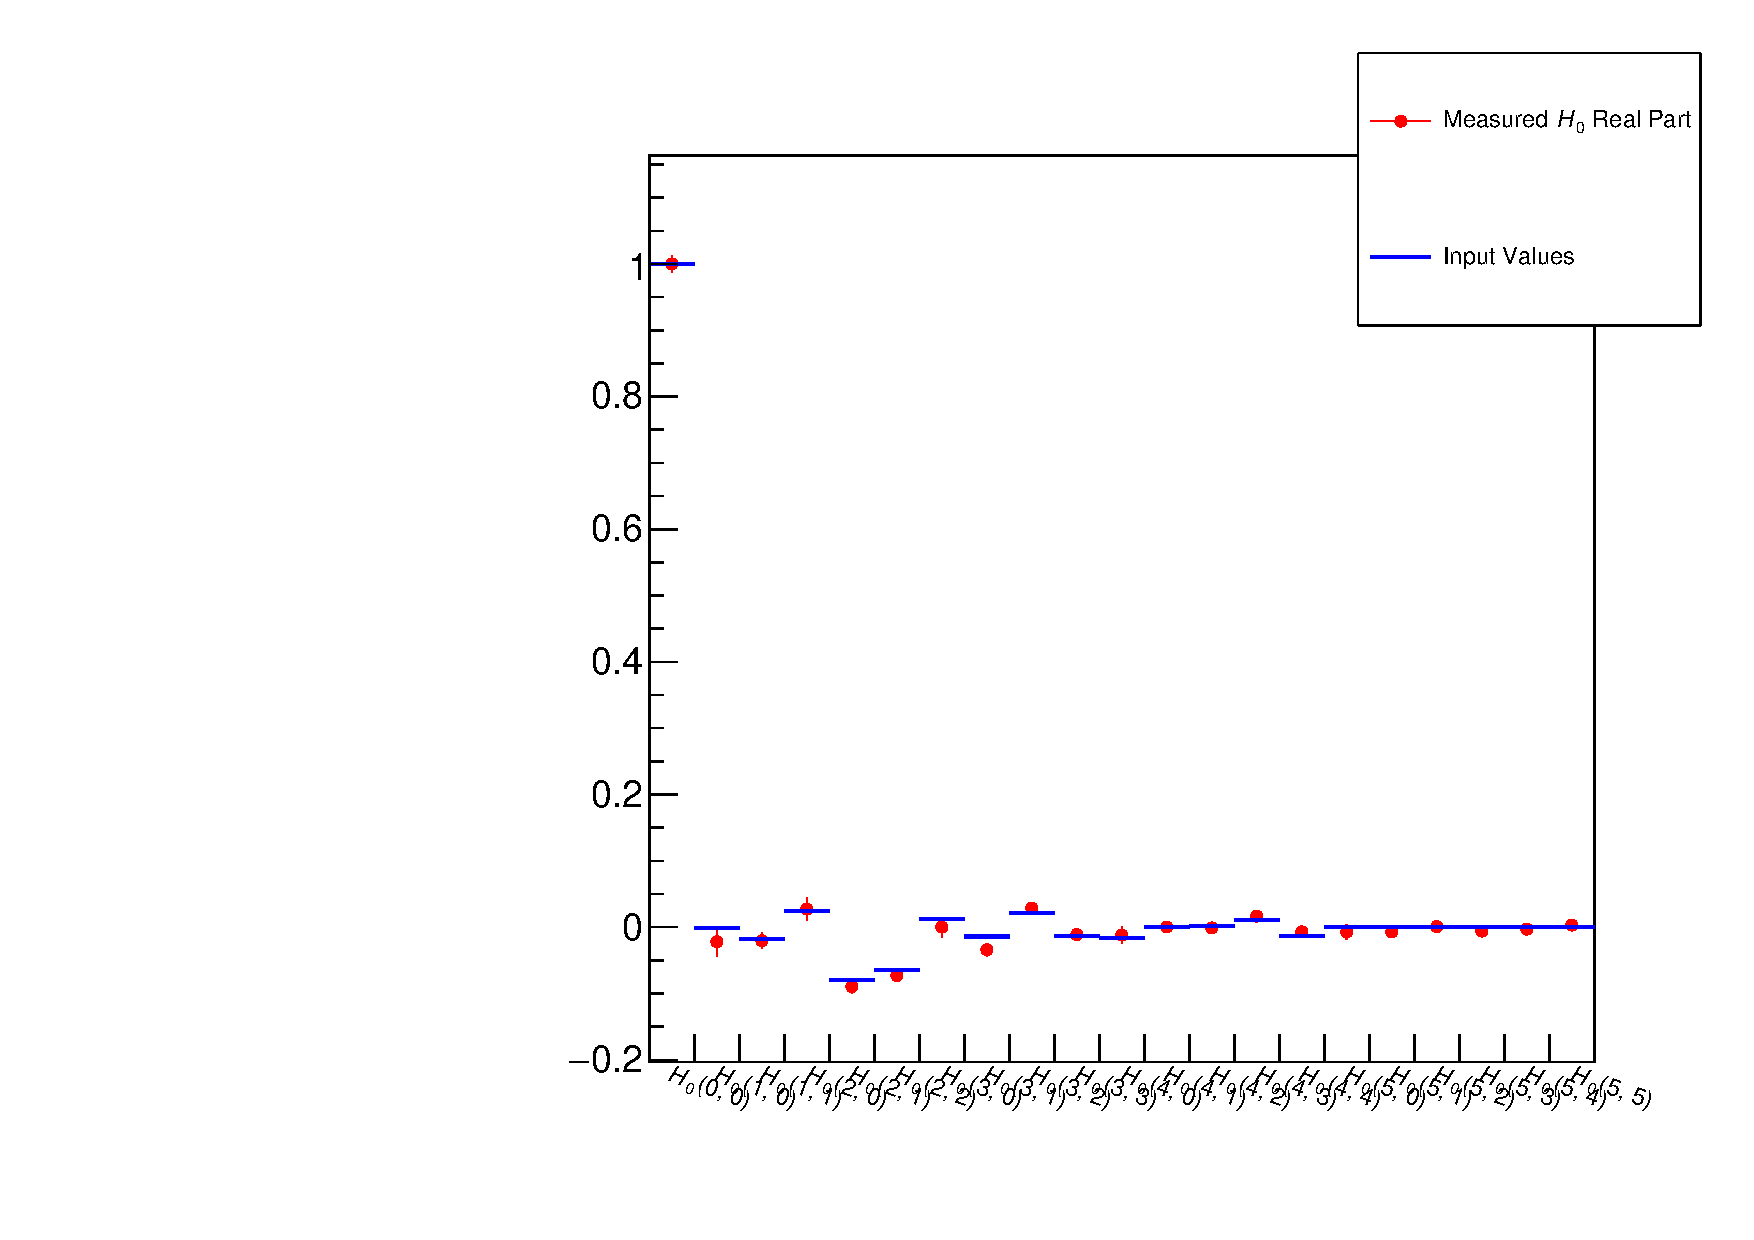
\includegraphics[width=0.5\textwidth]{photoprod/acc_1/hCompare_H0_Re}%
  }%
  \subfloat[][]{%
    \label{fig:photoprod_study_comparison_H0_im}%
    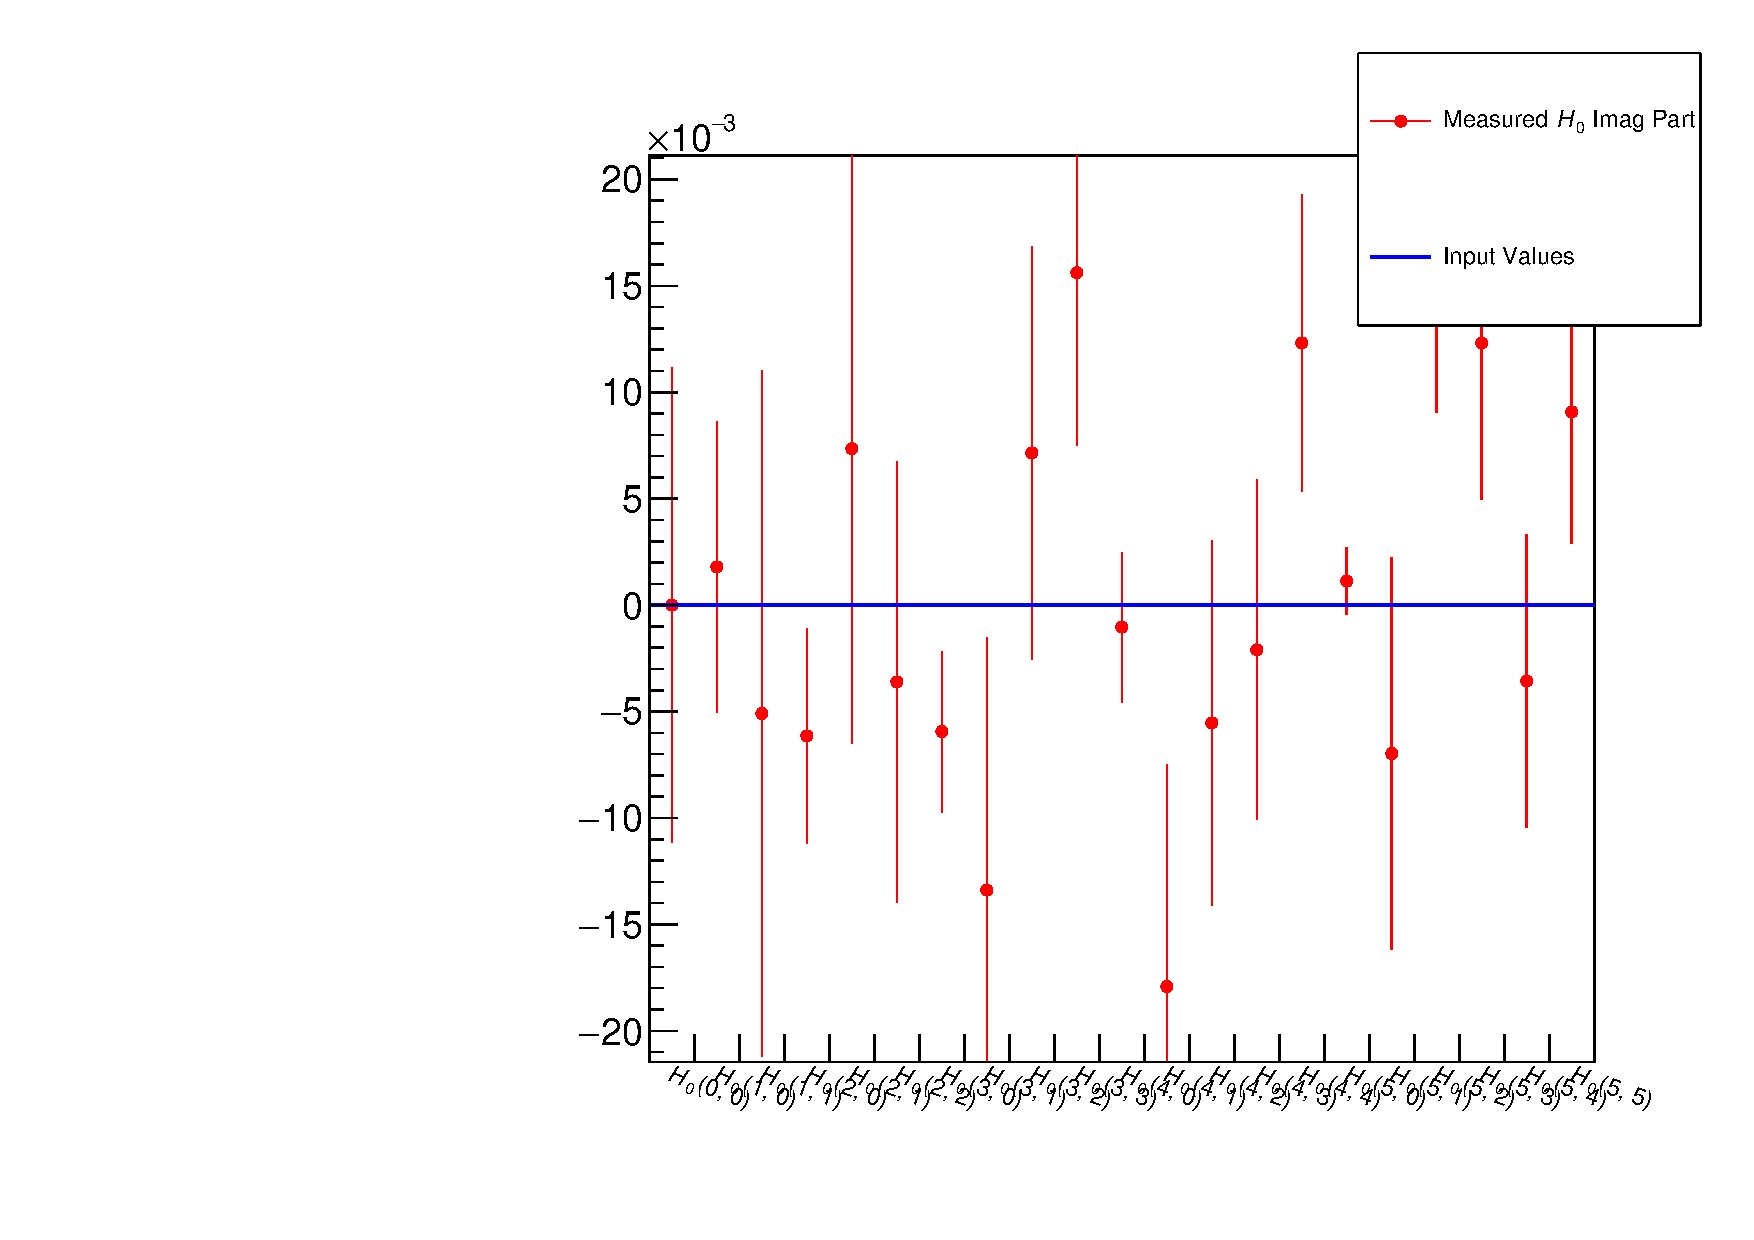
\includegraphics[width=0.5\textwidth]{photoprod/acc_1/hCompare_H0_Im}%
  }%
  \\%
  \subfloat[][]{%
    \label{fig:photoprod_study_residual_H0_re}%
    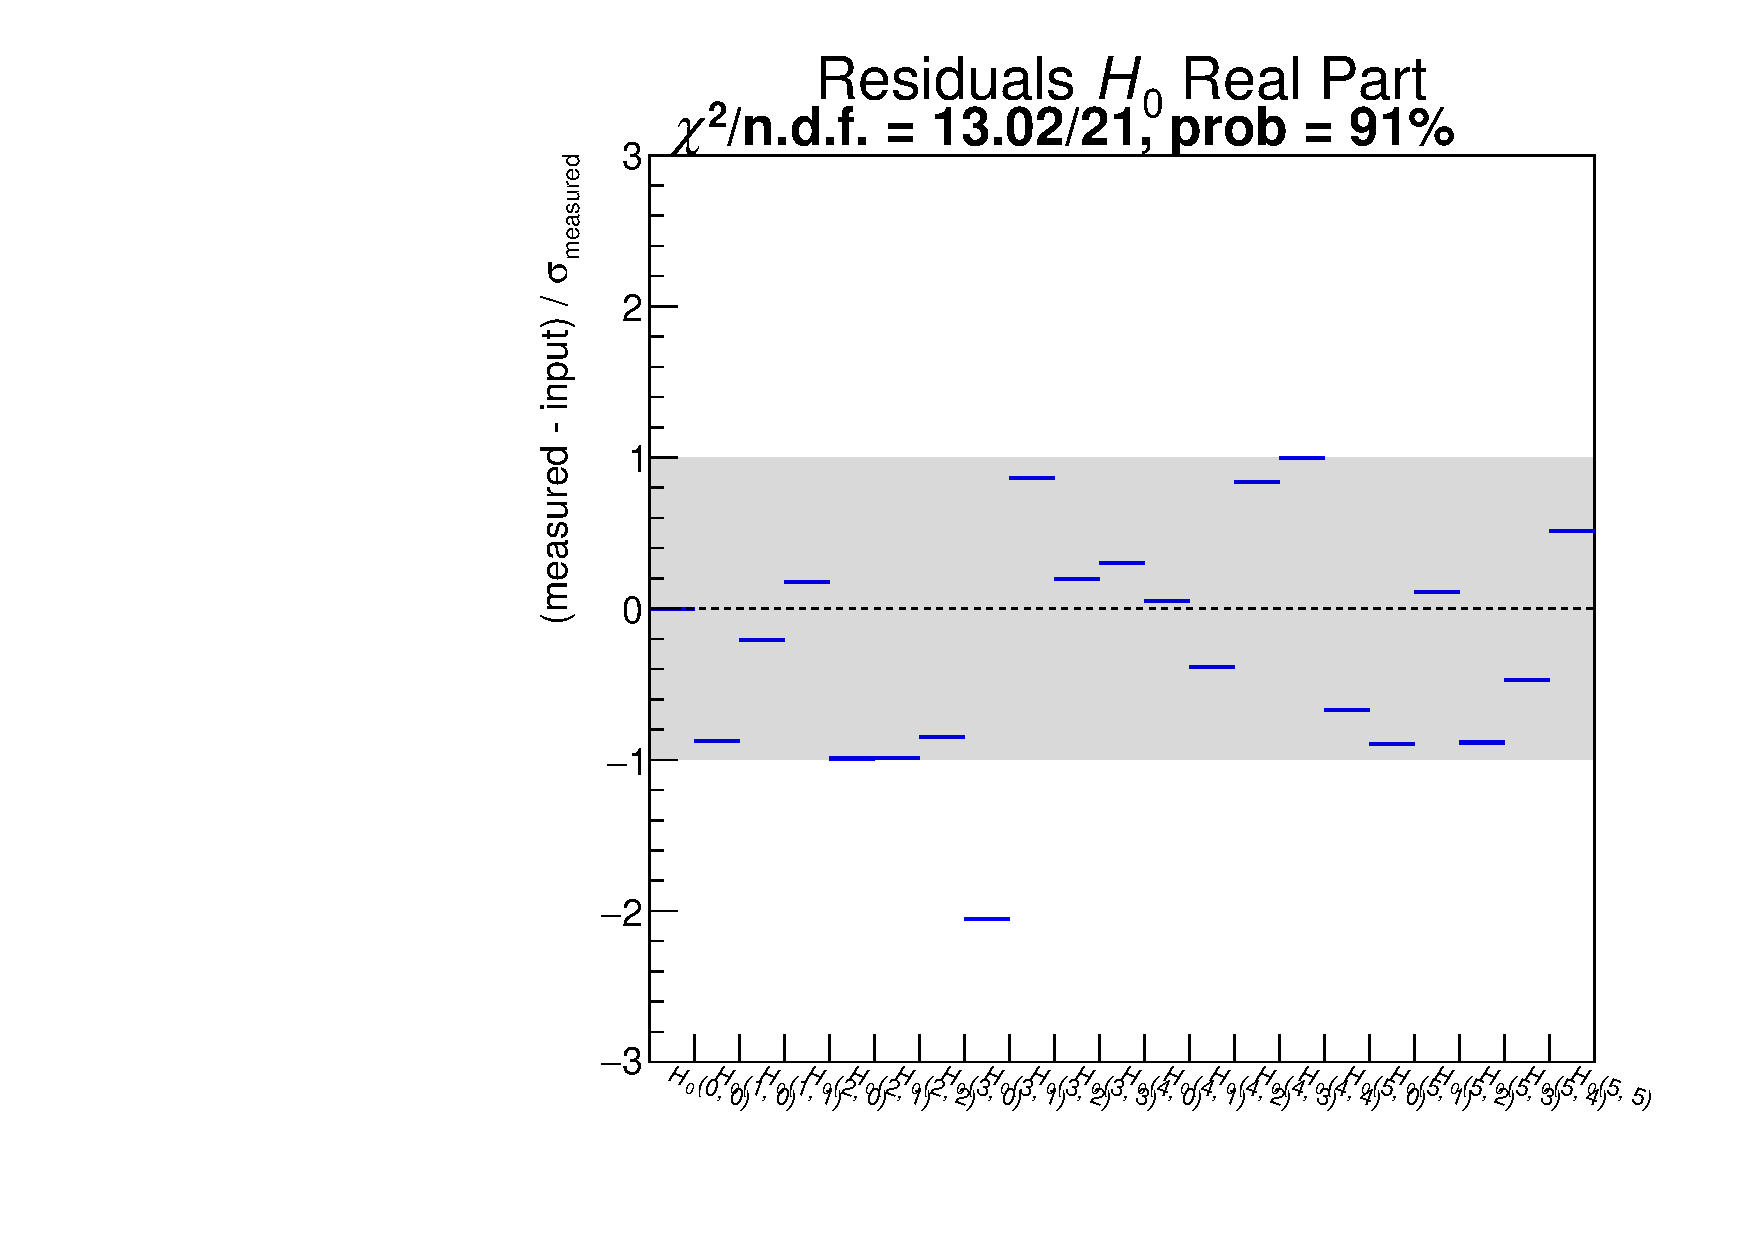
\includegraphics[width=0.5\textwidth]{photoprod/acc_1/hResiduals_H0_Re}%
  }%
  \subfloat[][]{%
    \label{fig:photoprod_study_residual_H0_im}%
    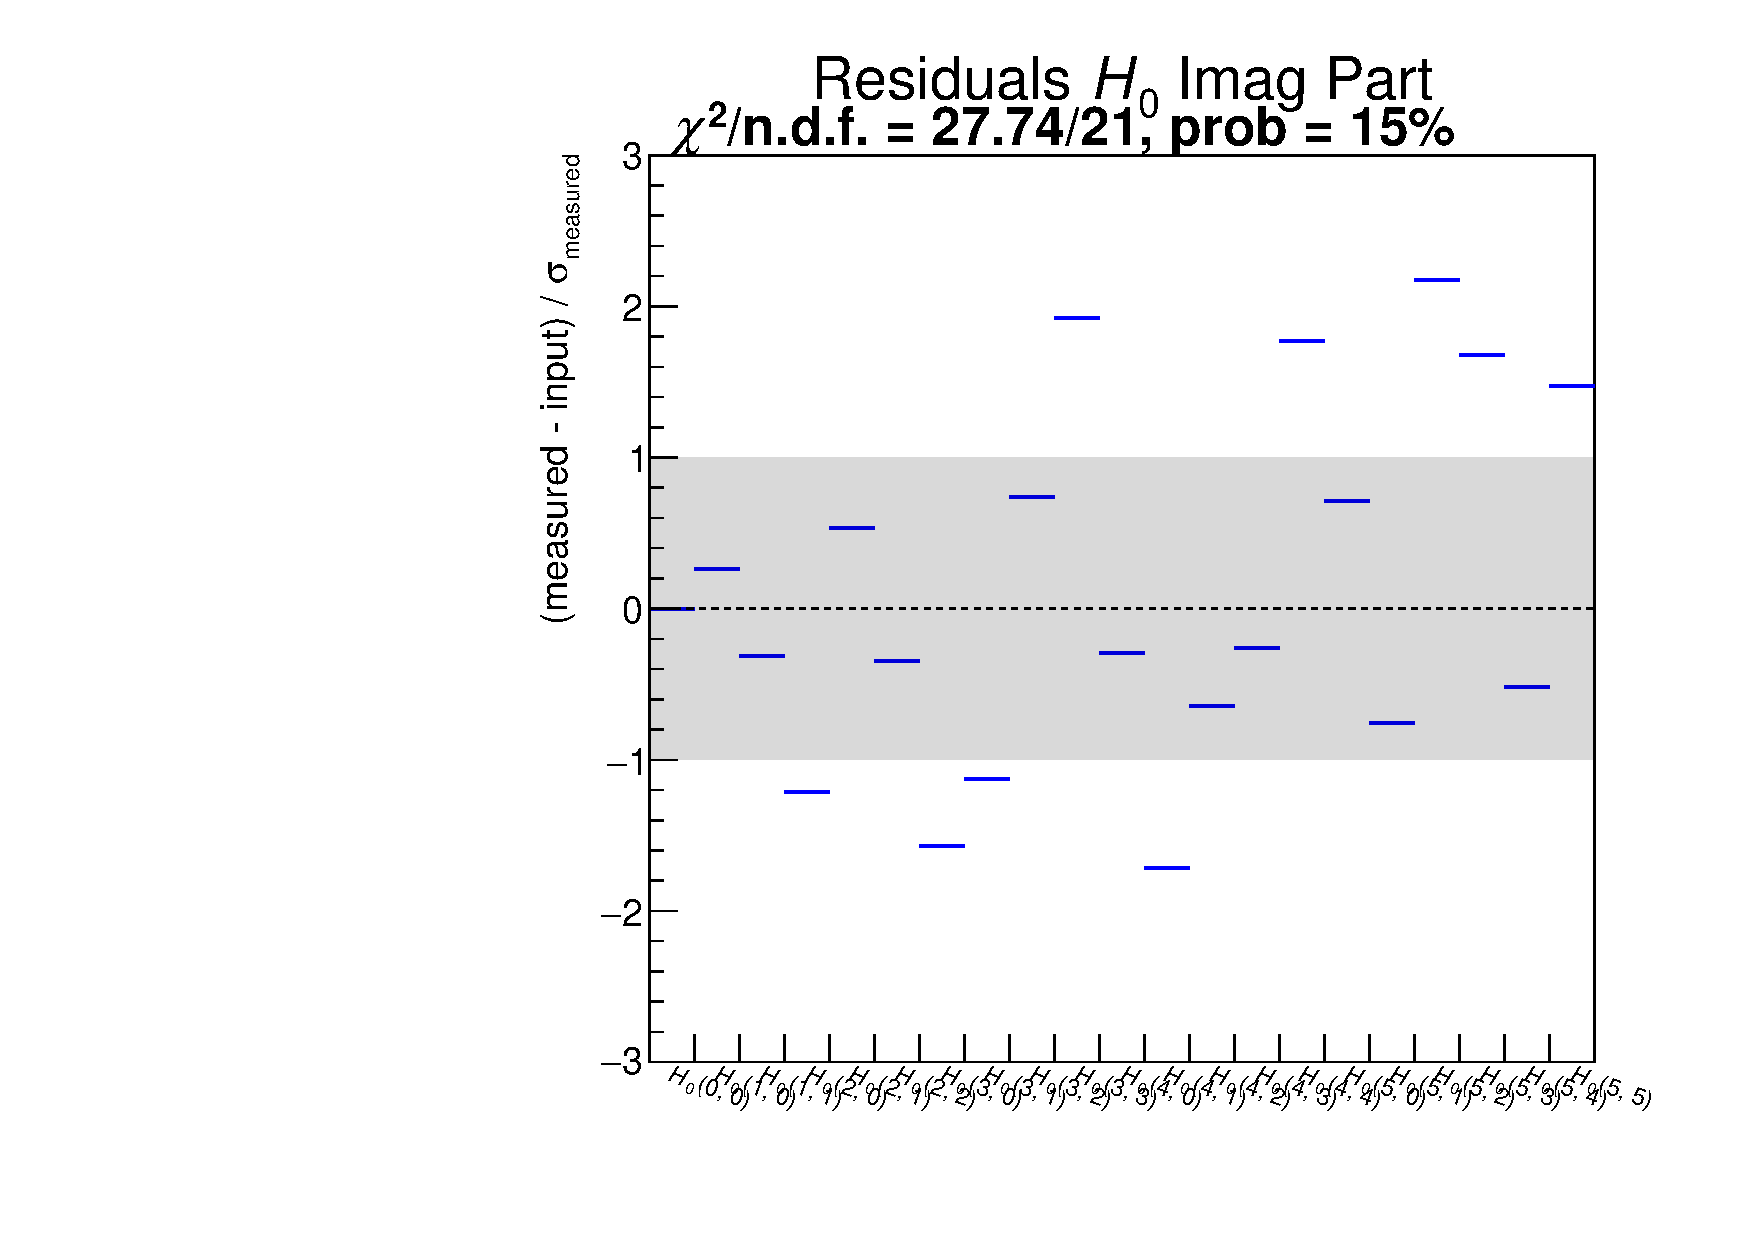
\includegraphics[width=0.5\textwidth]{photoprod/acc_1/hResiduals_H0_Im}%
  }%
  \caption{Upper row: Comparison of the physical moments $H_0(L, M)$
  (red points with uncertainties) extracted from the Monte Carlo data,
  which are generated using the partial-wave amplitudes in
  \cref{tab:photoprod_study_waveset} and the detection efficiency in
  \cref{eq:photoprod_study_acc1}, with the expected values (blue
  lines).  Both sets of values are normalized to the value of $H_0(0,
  0)$ in the respective set.
  \subfloatLabel{fig:photoprod_study_comparison_H0_re}~shows the real
  part of $H_0(L, M)$,
  \subfloatLabel{fig:photoprod_study_comparison_H0_im}~the imaginary
  part.  Note that moments with $L > 4$ are expected to be zero due to
  the chosen wave set.  Lower row: corresponding residuals.}%
  \label{fig:photoprod_study_output_H0}%
\end{figure}

\begin{figure}[tbp]
  \centering%
  \subfloat[][]{%
    \label{fig:photoprod_study_comparison_H1_re}%
    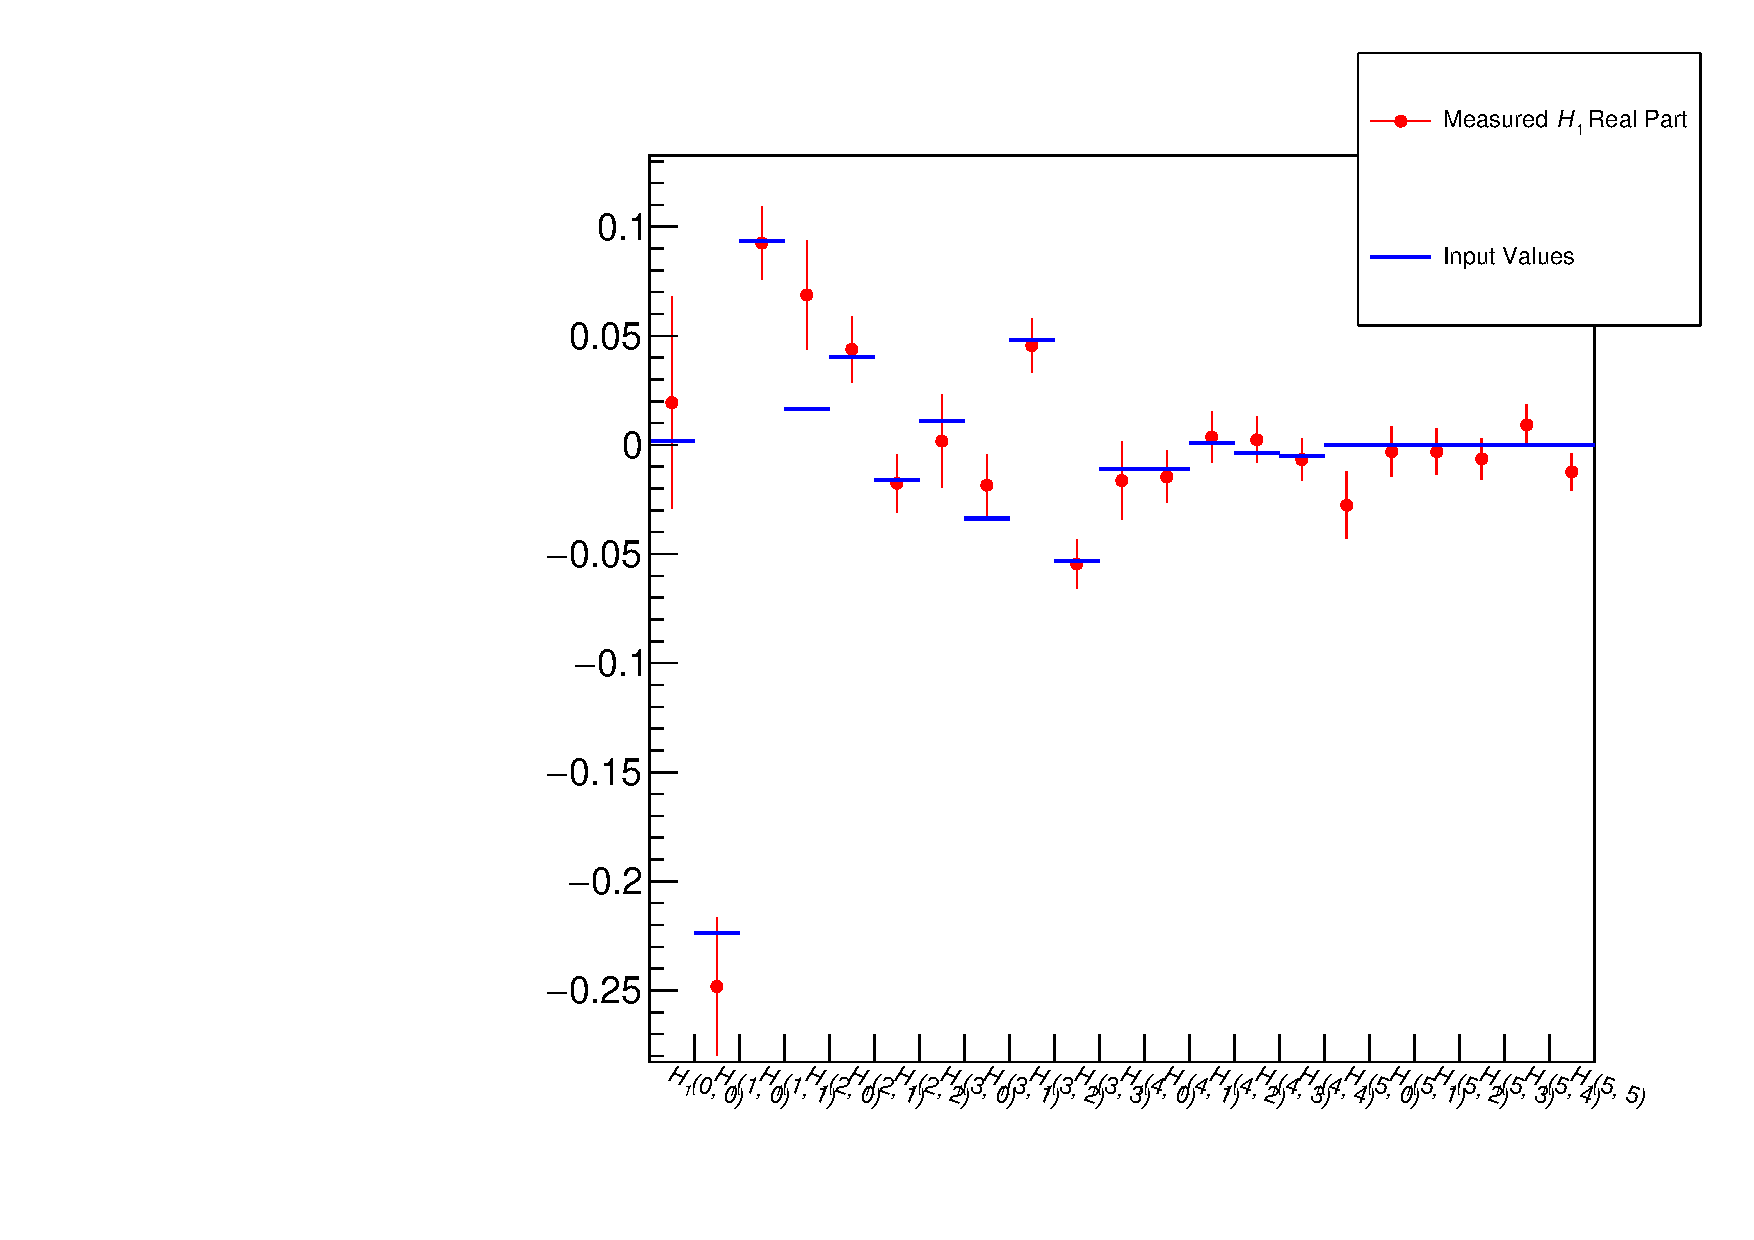
\includegraphics[width=0.5\textwidth]{photoprod/acc_1/hCompare_H1_Re}%
  }%
  \subfloat[][]{%
    \label{fig:photoprod_study_comparison_H1_im}%
    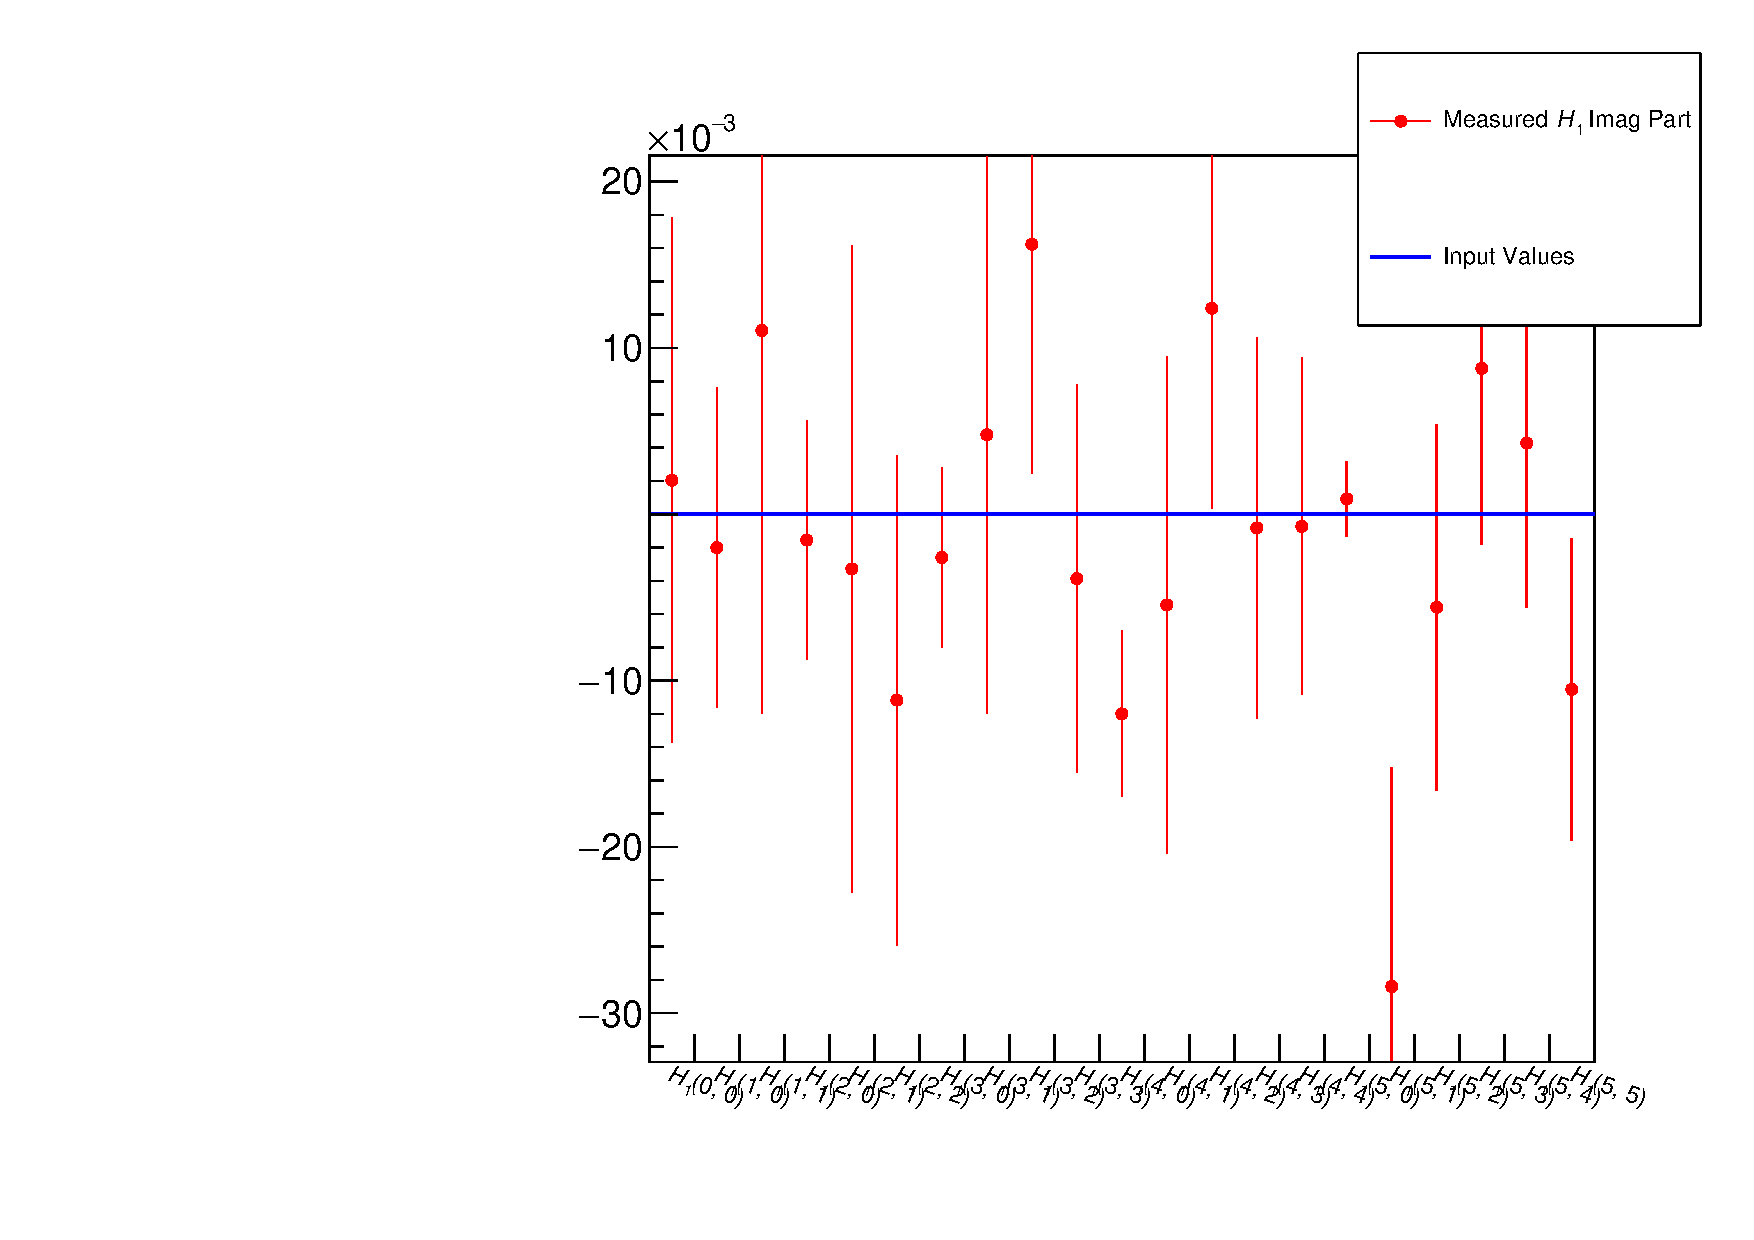
\includegraphics[width=0.5\textwidth]{photoprod/acc_1/hCompare_H1_Im}%
  }%
  \\%
  \subfloat[][]{%
    \label{fig:photoprod_study_residual_H1_re}%
    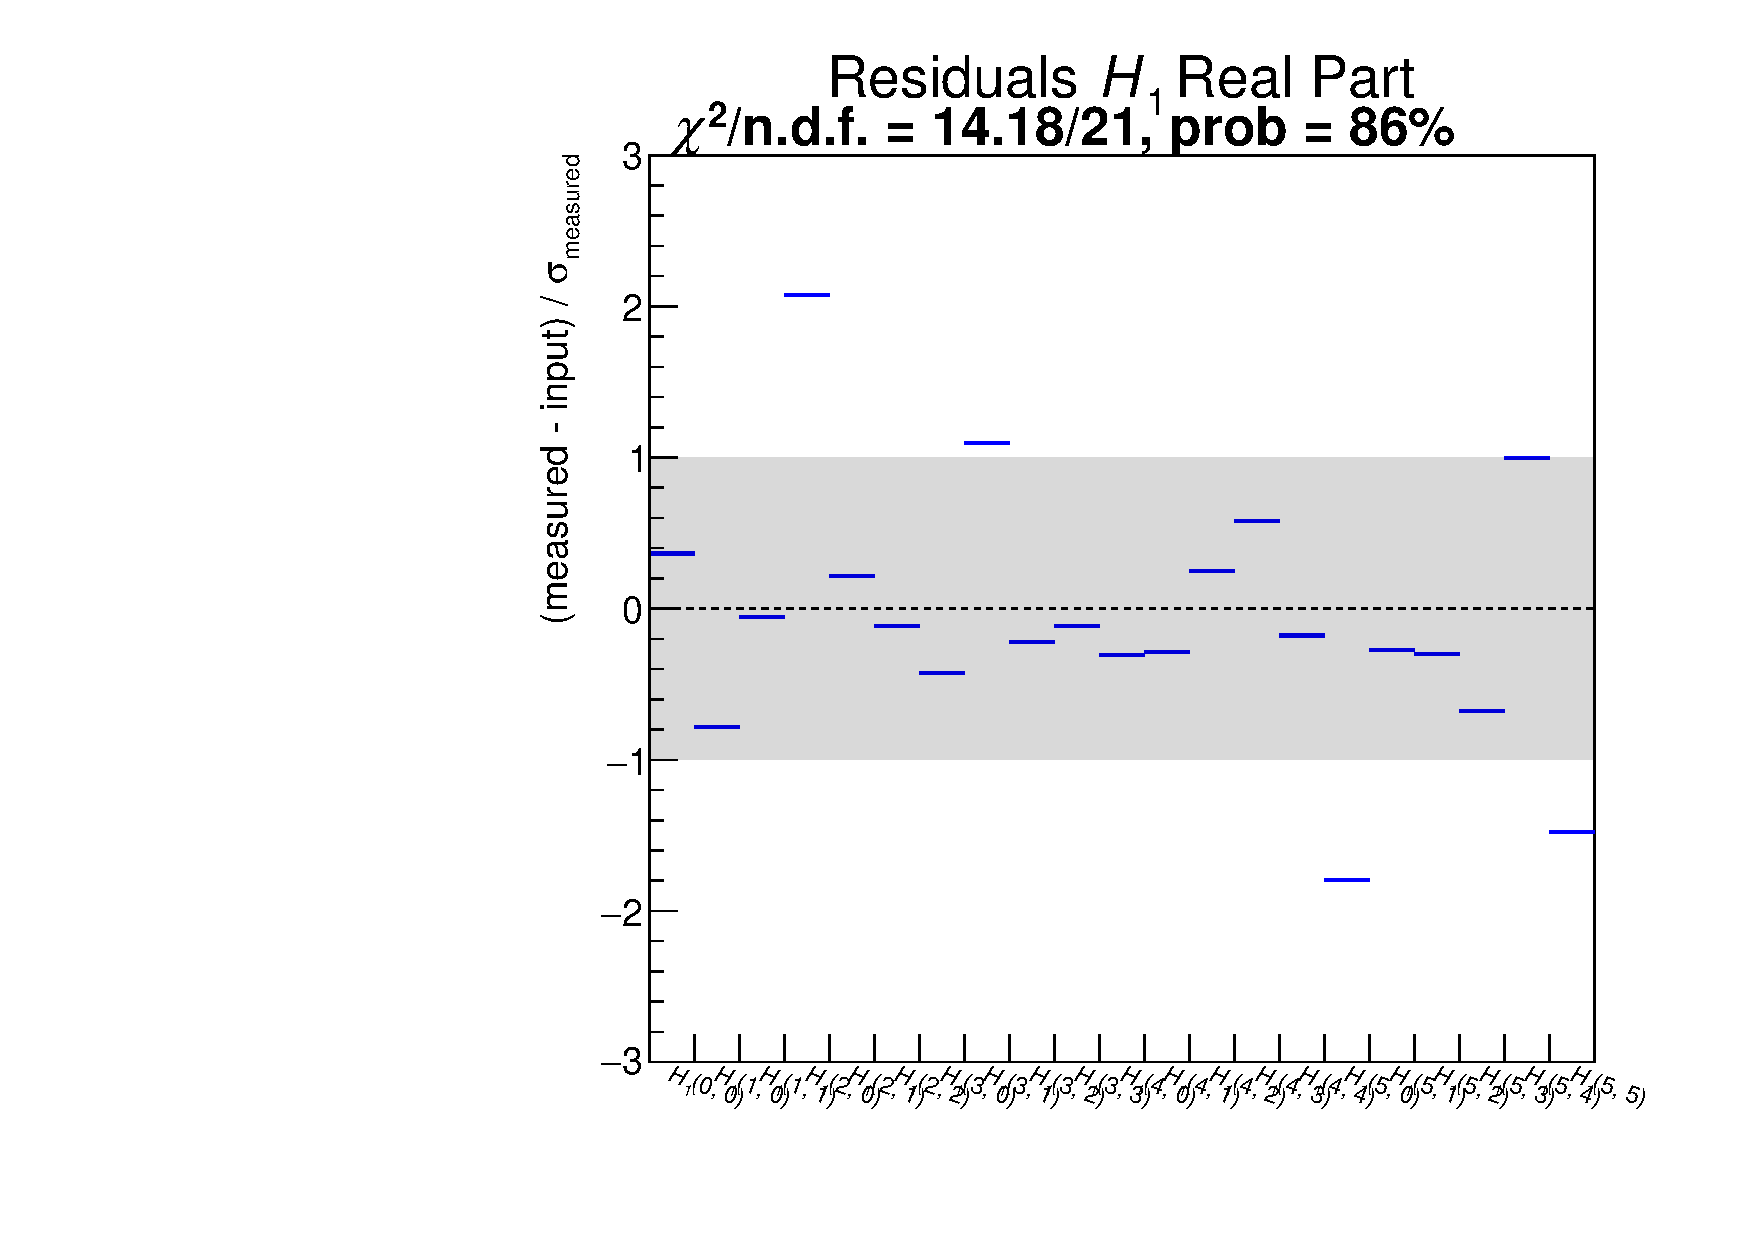
\includegraphics[width=0.5\textwidth]{photoprod/acc_1/hResiduals_H1_Re}%
  }%
  \subfloat[][]{%
    \label{fig:photoprod_study_residual_H1_im}%
    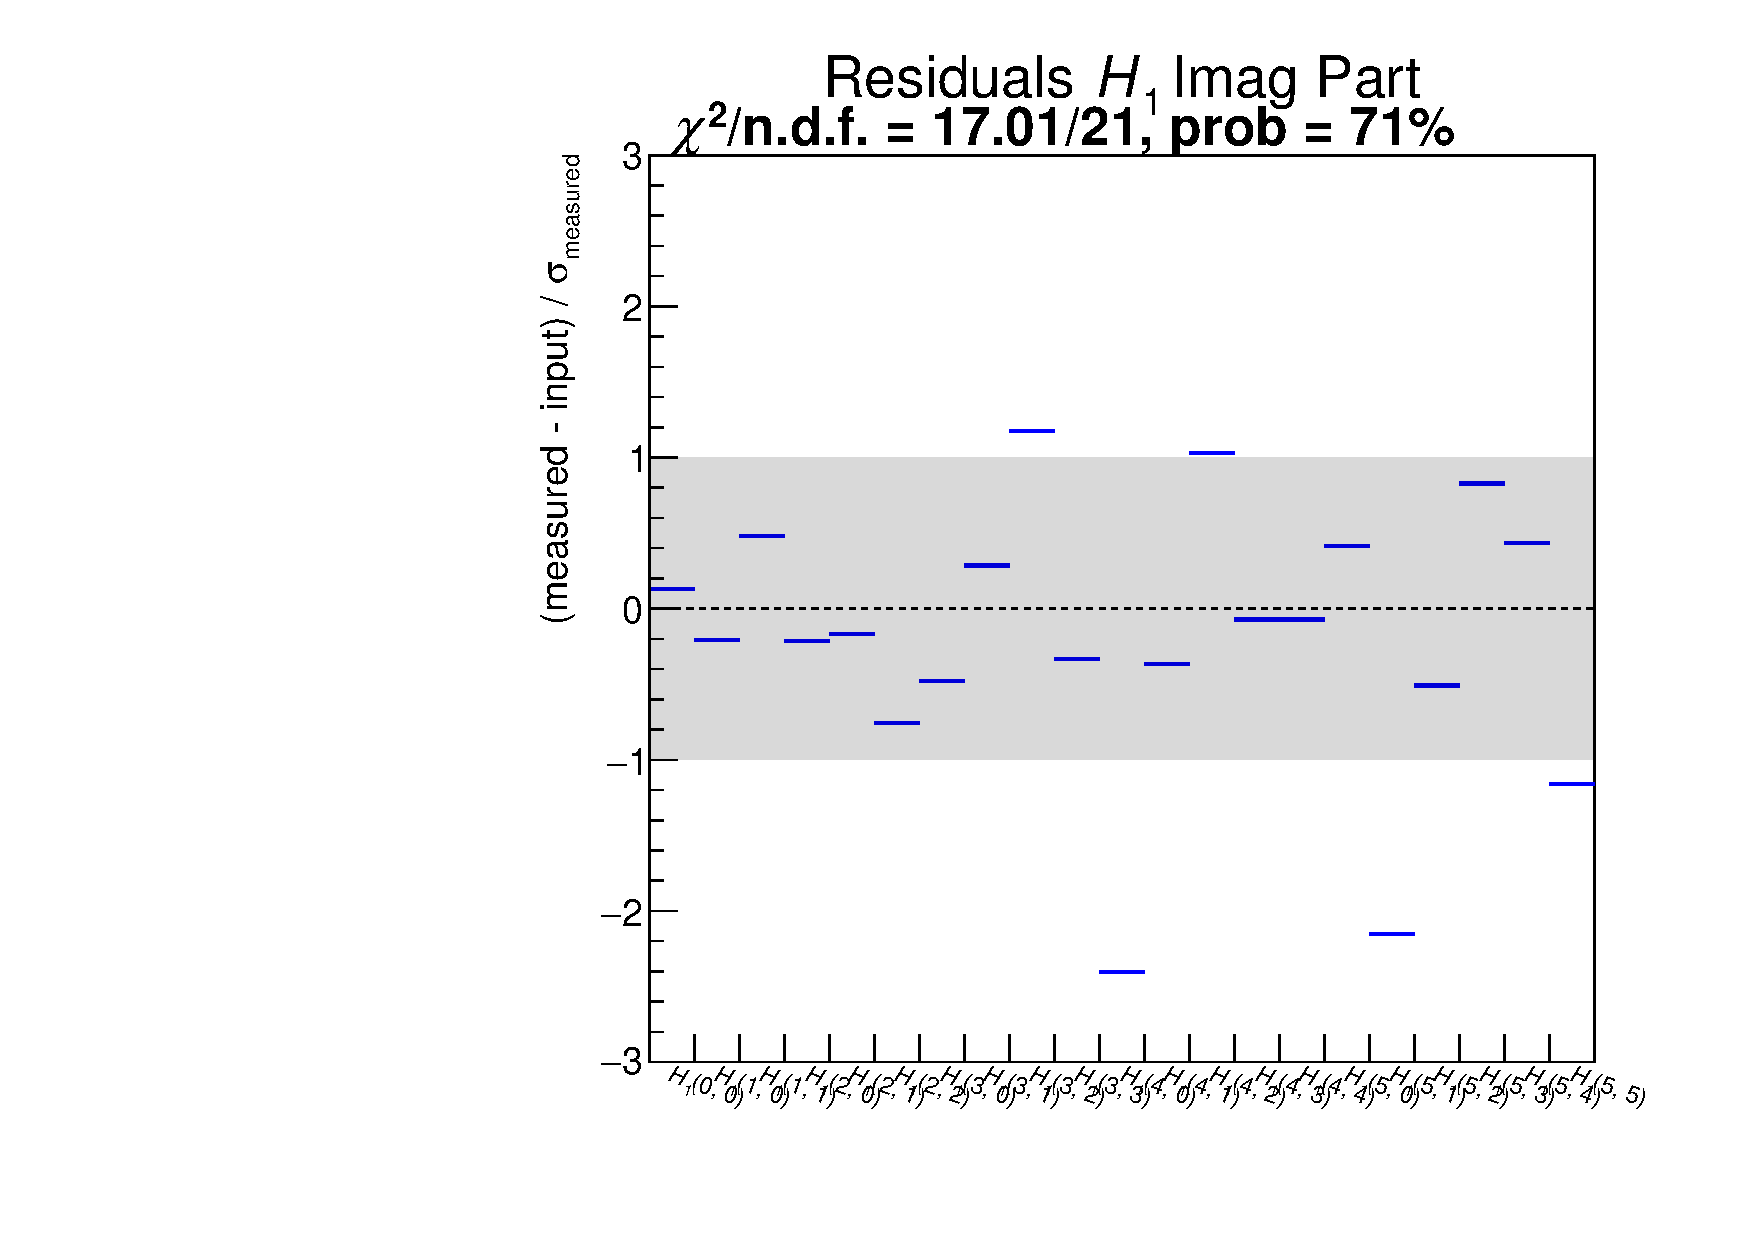
\includegraphics[width=0.5\textwidth]{photoprod/acc_1/hResiduals_H1_Im}%
  }%
  \caption{Same as \cref{fig:photoprod_study_output_H0} but for
  $H_1(L, M)$.}%
  \label{fig:photoprod_study_output_H1}%
\end{figure}

\begin{figure}[tbp]
  \centering%
  \subfloat[][]{%
    \label{fig:photoprod_study_comparison_H2_re}%
    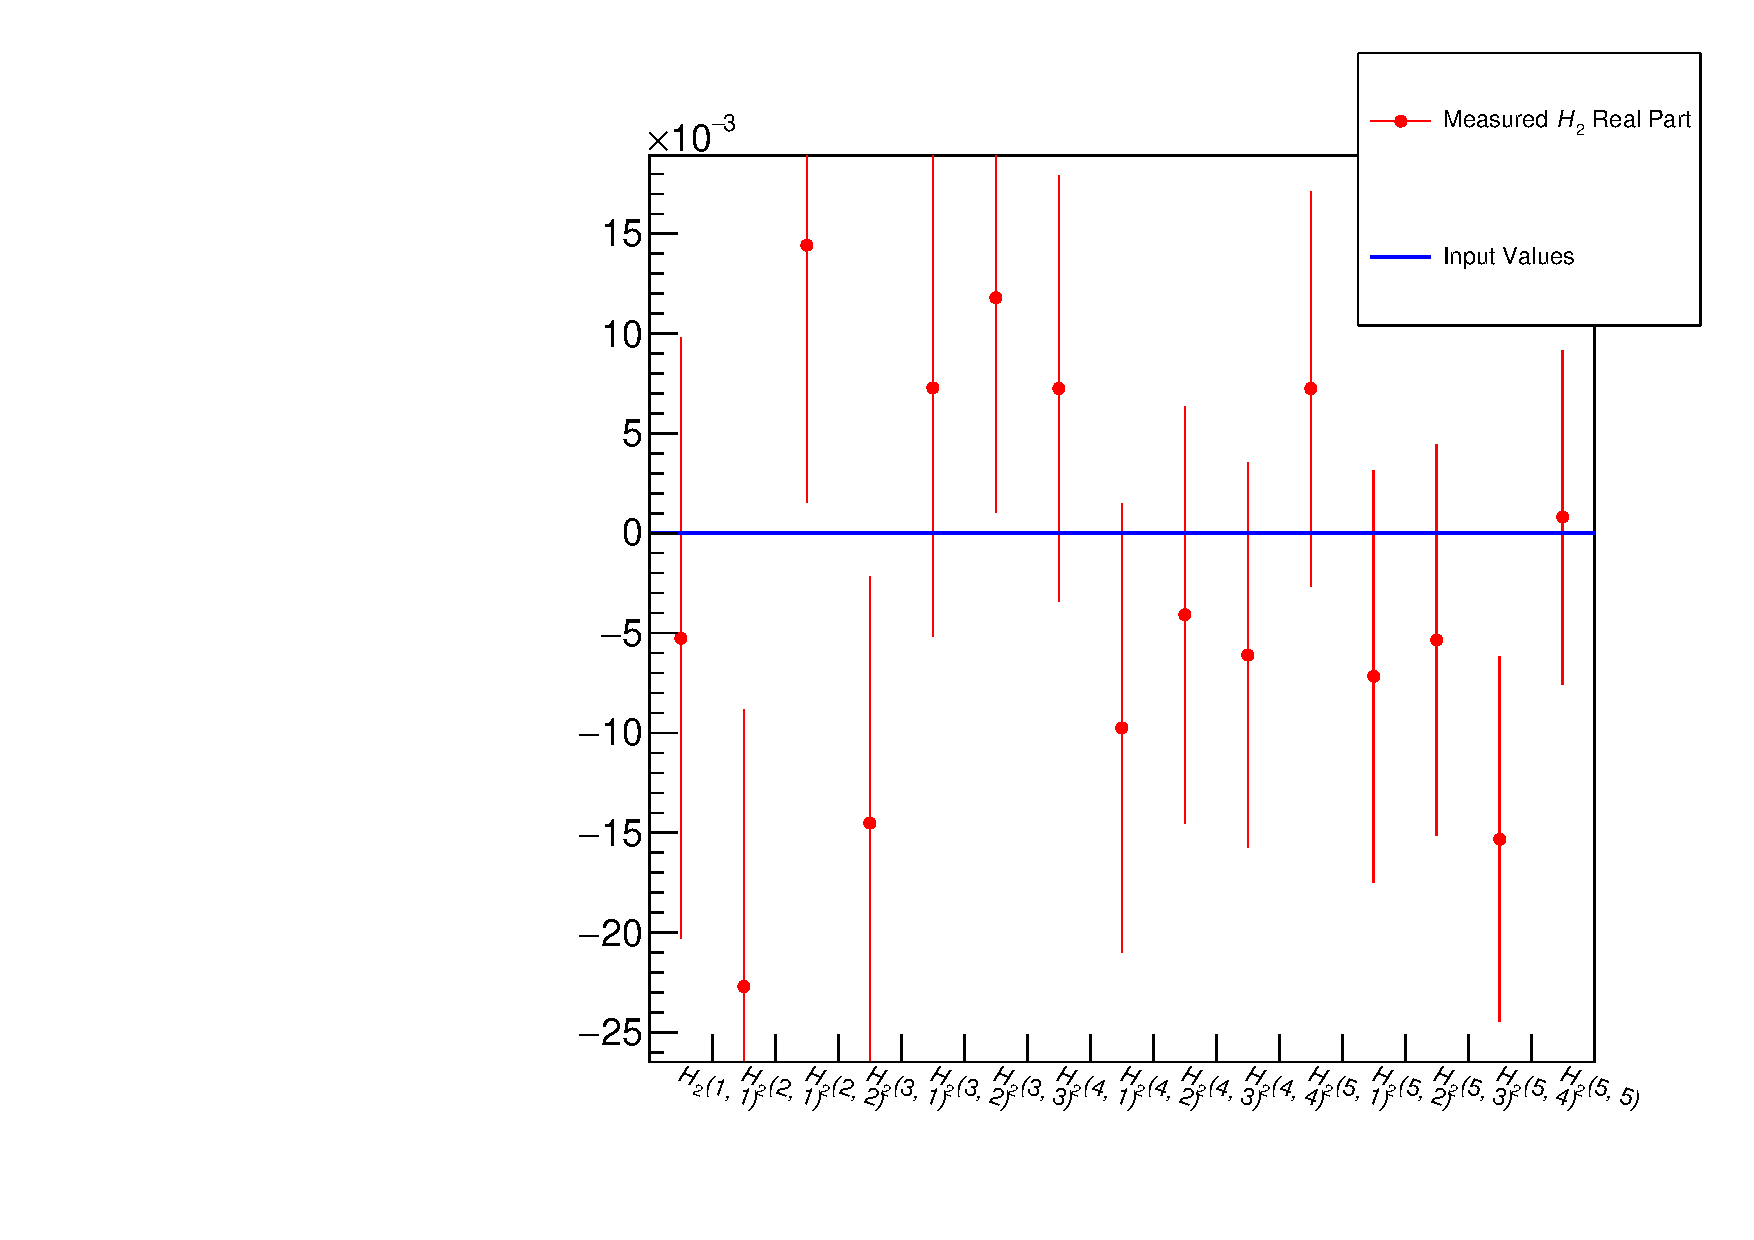
\includegraphics[width=0.5\textwidth]{photoprod/acc_1/hCompare_H2_Re}%
  }%
  \subfloat[][]{%
    \label{fig:photoprod_study_comparison_H2_im}%
    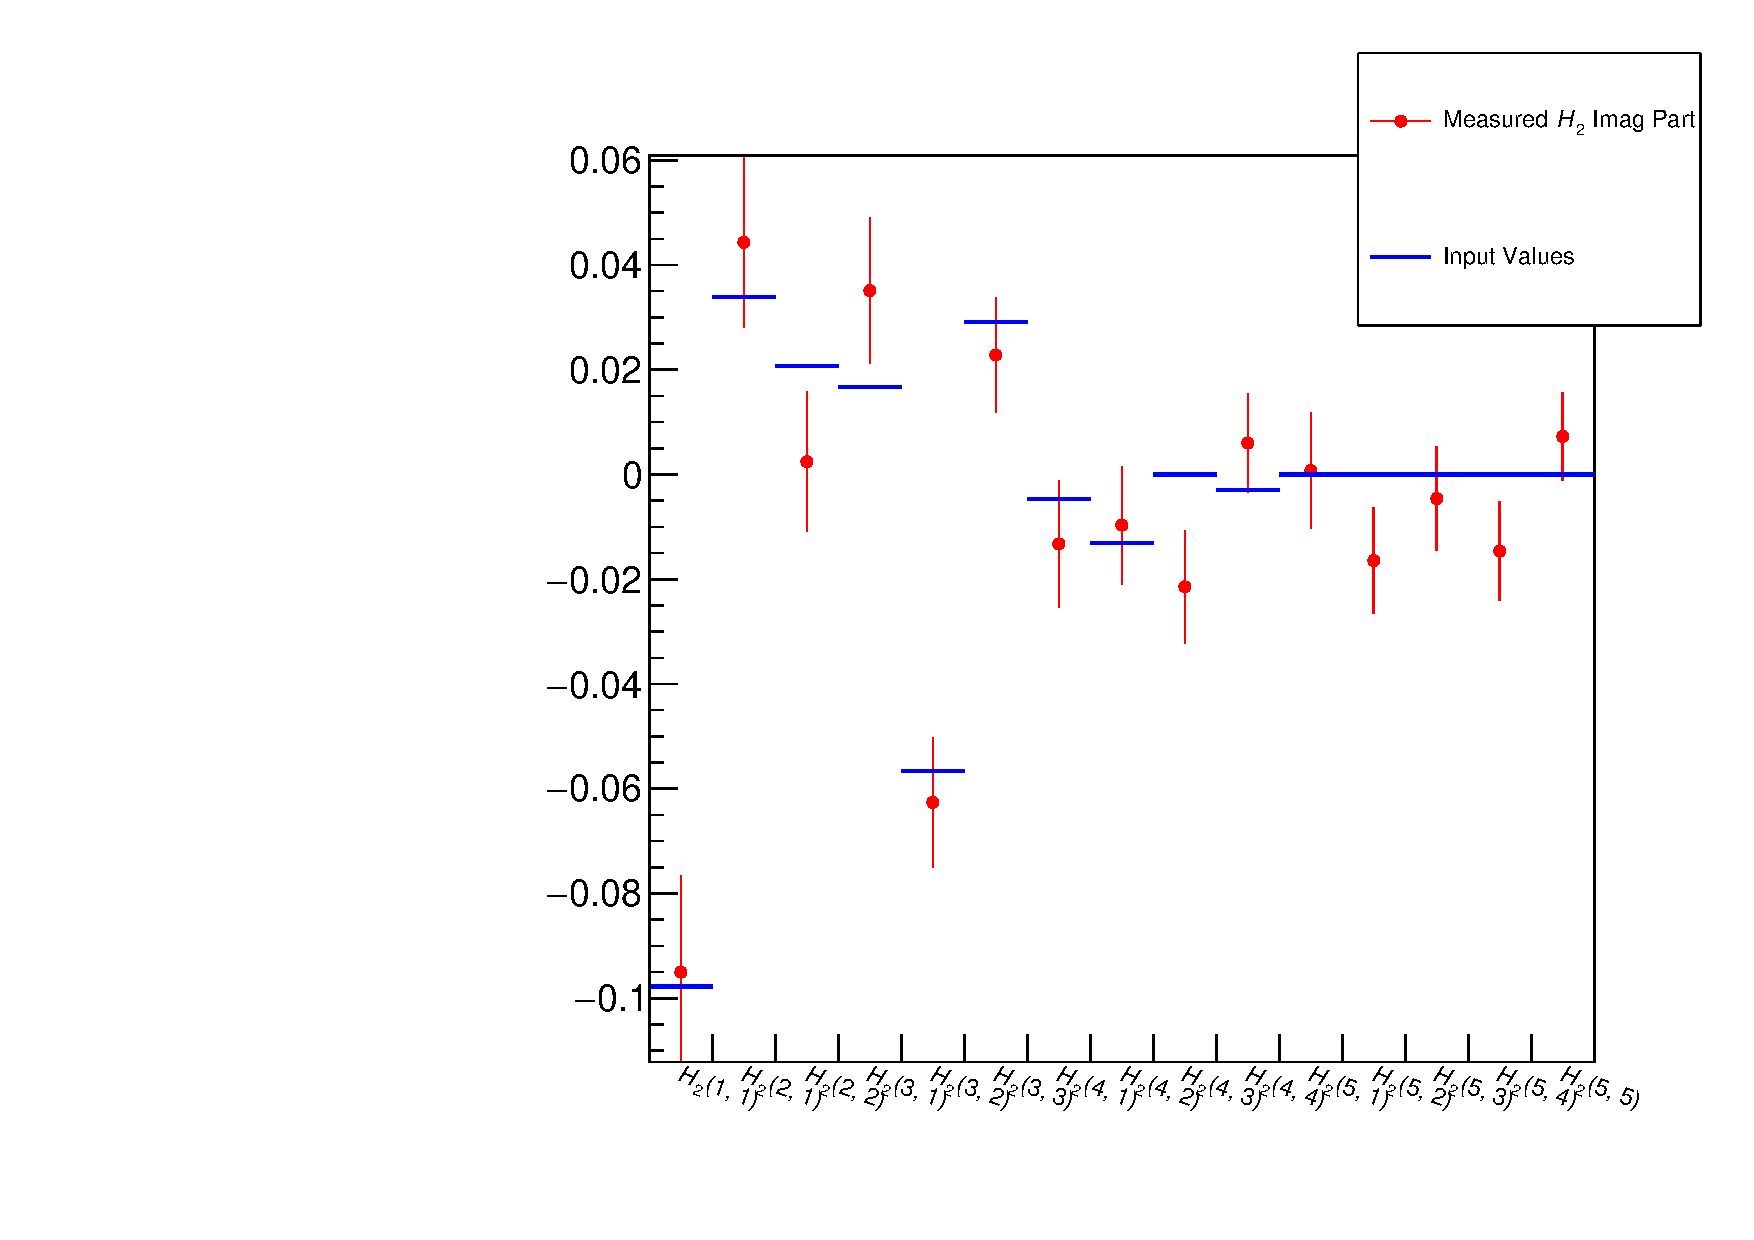
\includegraphics[width=0.5\textwidth]{photoprod/acc_1/hCompare_H2_Im}%
  }%
  \\%
  \subfloat[][]{%
    \label{fig:photoprod_study_residual_H2_re}%
    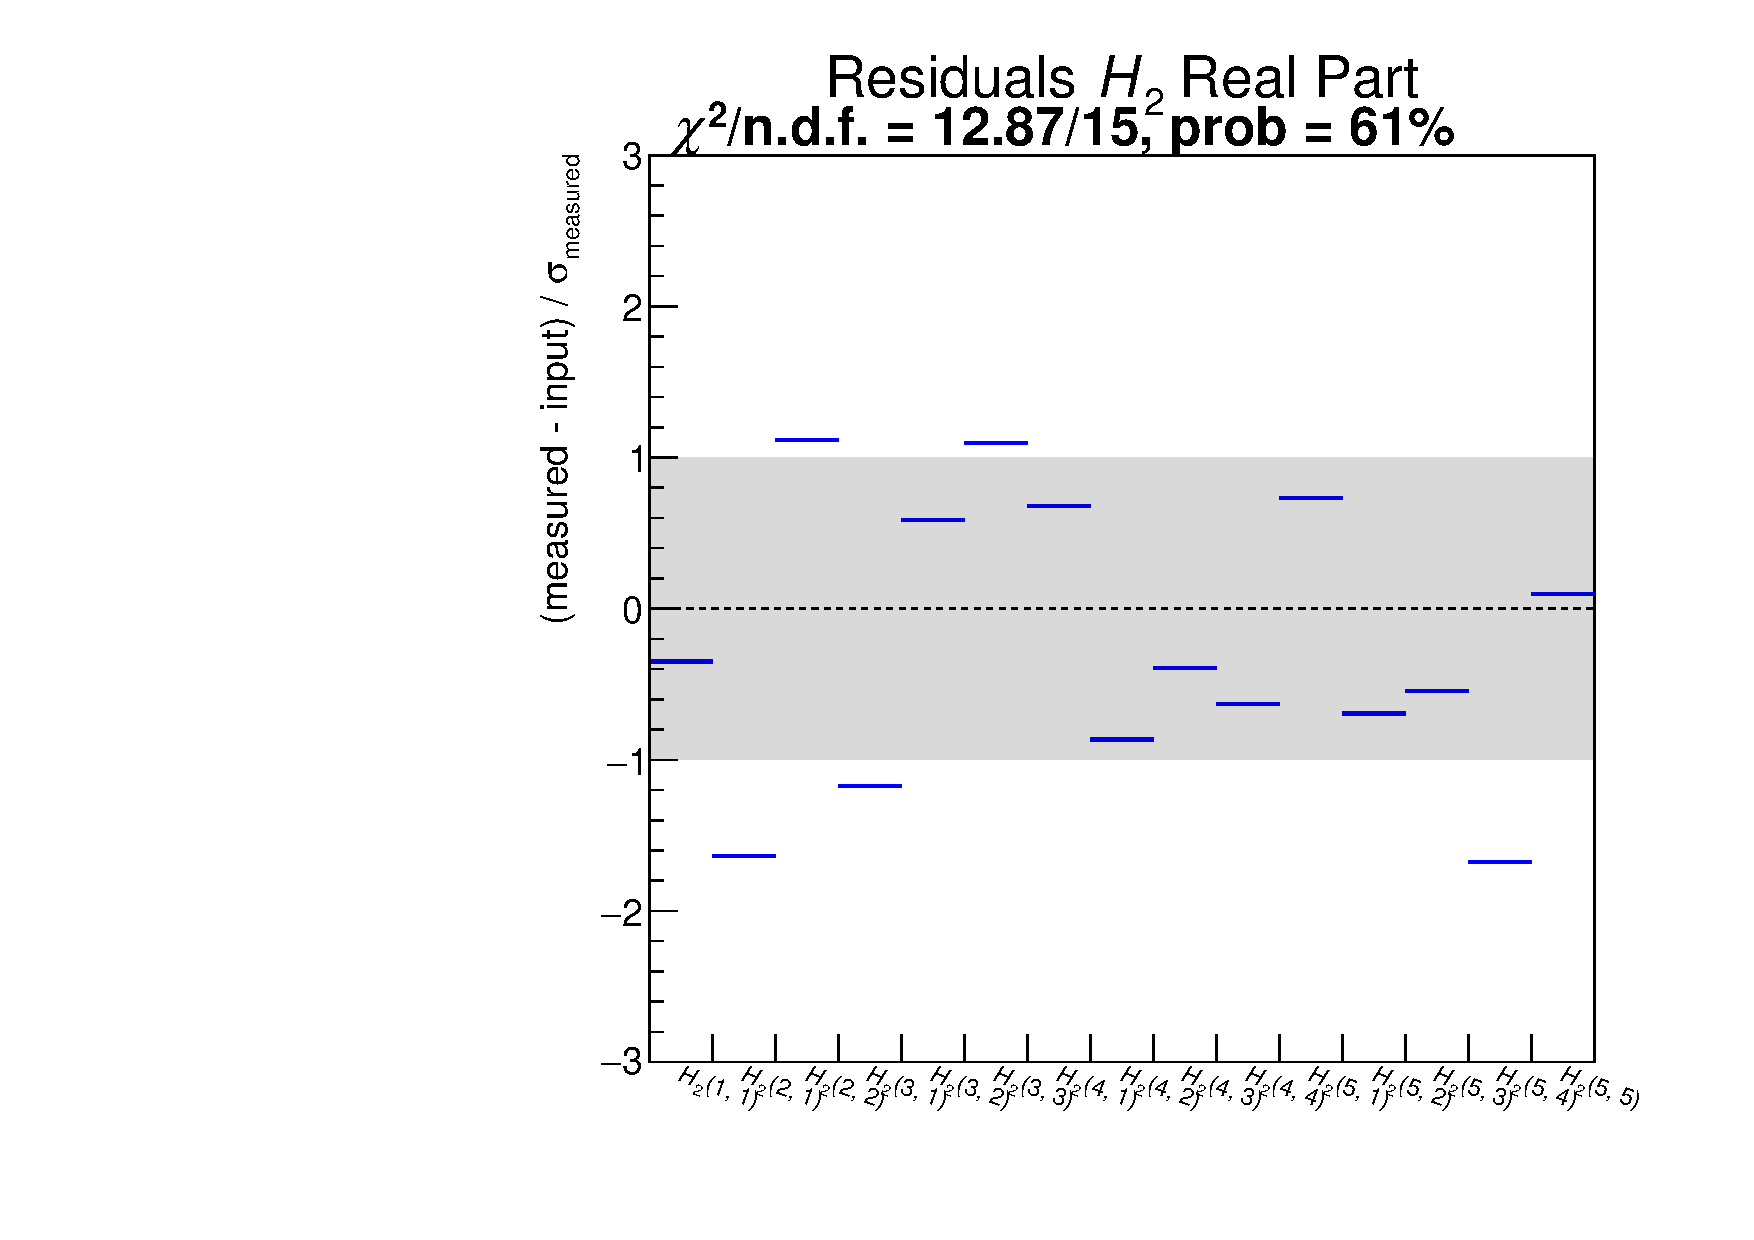
\includegraphics[width=0.5\textwidth]{photoprod/acc_1/hResiduals_H2_Re}%
  }%
  \subfloat[][]{%
    \label{fig:photoprod_study_residual_H2_im}%
    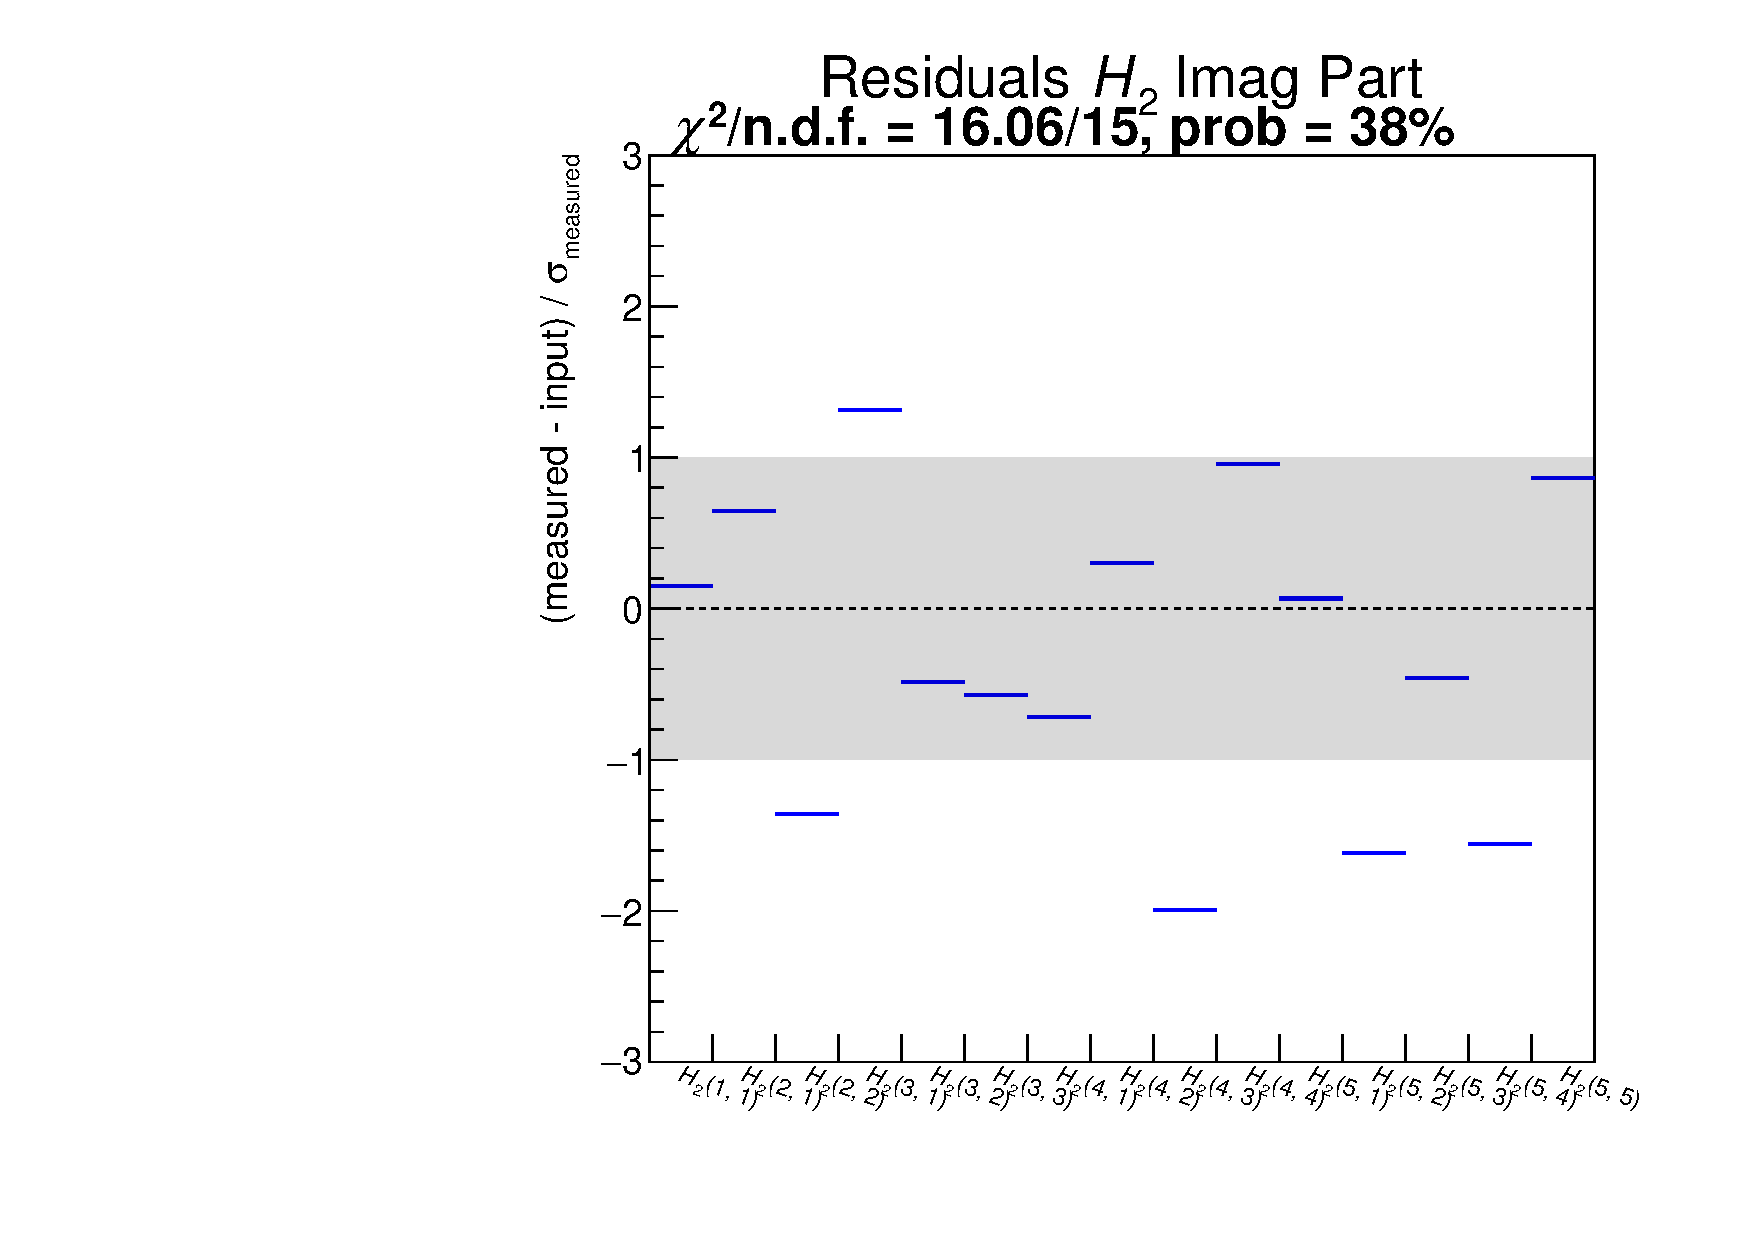
\includegraphics[width=0.5\textwidth]{photoprod/acc_1/hResiduals_H2_Im}%
  }%
  \caption{Same as \cref{fig:photoprod_study_output_H0} but for
  $H_2(L, M)$.}%
  \label{fig:photoprod_study_output_H2}%
\end{figure}


\clearpage
\subsubsection{Weighted events}%
\label{sec:photoprod:example_weighted}

To test the case of weighted events, we perform a Monte Carlo
input-output study where the physical intensity distribution is given
by the sum of a signal and a background contribution, which both have
different angular distributions.  The angular distribution of the
signal is defined by the same partial-wave amplitudes already used in
\cref{sec:photoprod:example_unweighted} (see
\cref{tab:photoprod_study_waveset}).  For the angular distribution of
the background component, we use the same set of waves, but different
amplitude values, which are listed in
\cref{tab:photoprod_study_waveset_bkg}.  In both cases, we again
assume ideal beam-photon polarization, \ie $P_\gamma = 1$.  The two
angular distributions of the intensity components are shown in
\cref{fig:photoprod_study_weighted_intensity_sig,fig:photoprod_study_weighted_intensity_bkg}.

\begin{table}[tbp]
  \centering%
  \renewcommand{\arraystretch}{1.2}%
  \caption{Partial-wave amplitude values used to generate pseudodata
  for the background component.  The wave notation is
  $\ell_m^{(\refl)}$.}%
  \label{tab:photoprod_study_waveset_bkg}%
  \vspace*{1ex}%
  \hfill%
  \begin{tabular}{ll}
    \toprule
    \textbf{Partial wave} &
    \textbf{Amplitude value} \\
    \midrule
    % negative-reflectivity waves
    $S_0^{(-)}$    & $\hphantom{-}1.0$ \\
    $P_{-1}^{(-)}$ & $-0.9 + 0.7 \imag$ \\
    $P_0^{(-)}$    & $-0.6 + 0.4 \imag$ \\
    $P_{+1}^{(-)}$ & $-0.9 - 0.8 \imag$ \\
    $D_{-2}^{(-)}$ & $-1.0 - 0.7 \imag$ \\
    $D_{-1}^{(-)}$ & $-0.8 - 0.7 \imag$ \\
    $D_0^{(-)}$    & $\hphantom{-}0.4 + 0.3 \imag$ \\
    $D_{+1}^{(-)}$ & $-0.6 - 0.1 \imag$ \\
    $D_{+2}^{(-)}$ & $-0.1 - 0.9 \imag$ \\
    \bottomrule
  \end{tabular}
  \hfill%
  \begin{tabular}{ll}
    \toprule
    \textbf{Partial wave} &
    \textbf{Amplitude value} \\
    \midrule
    % positive-reflectivity waves
    $S_0^{(+)}$    & $\hphantom{-}0.5$ \\
    $P_{-1}^{(+)}$ & $-1.0 + 0.8 \imag$ \\
    $P_0^{(+)}$    & $-0.2 + 0.2 \imag$ \\
    $P_{+1}^{(+)}$ & $\hphantom{-}0.0 - 0.3 \imag$ \\
    $D_{-2}^{(+)}$ & $\hphantom{-}0.7 + 0.9 \imag$ \\
    $D_{-1}^{(+)}$ & $-0.4 - 0.5 \imag$ \\
    $D_0^{(+)}$    & $-0.3 + 0.2 \imag$ \\
    $D_{+1}^{(+)}$ & $-1.0 - 0.4 \imag$ \\
    $D_{+2}^{(+)}$ & $\hphantom{-}0.5 - 0.2 \imag$ \\
    \bottomrule
  \end{tabular}
  \hfill\null%
\end{table}

\begin{figure}[tbp]
  \centering%
  \subfloat[][]{%
    \label{fig:photoprod_study_weighted_intensity_sig}%
    \includegraphics[width=0.5\textwidth]{photoprod_weighted/no_acc/intensitySig}%
  }%
  \subfloat[][]{%
    \label{fig:photoprod_study_weighted_intensity_bkg}%
    \includegraphics[width=0.5\textwidth]{photoprod_weighted/no_acc/intensityBkg}%
  }%
  \\%
  \subfloat[][]{%
    \label{fig:photoprod_study_weighted_data_10M}%
    \includegraphics[width=0.5\textwidth]{photoprod_weighted/no_acc_10M/data}%
  }%
  \subfloat[][]{%
    \label{fig:photoprod_study_weighted_discr_var_10M}%
    \includegraphics[width=0.5\textwidth]{photoprod_weighted/no_acc_10M/hDiscrVariableSim}%
  }%
  \caption{\subfloatLabel{fig:photoprod_study_weighted_intensity_sig}~Intensity
  distribution used to generate the signal component as defined by the
  partial-wave amplitudes listed in
  \cref{tab:photoprod_study_waveset}.
  \subfloatLabel{fig:photoprod_study_weighted_intensity_bkg}~Intensity
  distribution used to generate the background component as defined by
  the partial-wave amplitudes listed in
  \cref{tab:photoprod_study_waveset_bkg}.
  \subfloatLabel{fig:photoprod_study_weighted_data_10M}~Total Monte
  Carlo data sample obtained by randomly drawing \num{e7}~events from
  each of the distributions
  in~\subfloatLabel{fig:photoprod_study_weighted_intensity_sig}
  and~\subfloatLabel{fig:photoprod_study_weighted_intensity_bkg}.
  \subfloatLabel{fig:photoprod_study_weighted_discr_var_10M}~Distribution
  of the discriminatory variable for the total Monte Carlo data sample
  in~\subfloatLabel{fig:photoprod_study_weighted_data_10M}.  The
  shaded regions indicate the signal and side bands.}%
  \label{fig:photoprod_study_weighted}%
\end{figure}

The angular distributions are disentangled by applying a
one-dimensional sideband subtraction in a hypothetical discriminating
variable, which covers the range $[-1, +1]$.\footnote{In practice,
this could be, for example, the invariant mass distribution of an
unstable daughter particle.}  In this variable, the signal is
generated according to a Gaussian, which is centered at~0 and has a
standard deviation of~0.1, while the background is generated
uniformly.  The signal band in the discriminating variable is $[-0.3,
+0.3]$.  Events in this range, are assigned a weight of $w_k = +1$.
The sidebands are $[-1.0, -0.4]$ and $[+0.4, +1.0]$.  Events in these
ranges are assigned a weight of $w_k = -1/2$.\todo{add bands as well
as signal and background components to
\cref{fig:photoprod_study_weighted_discr_var_10M}}

To verify that the sideband subtraction works, we generate a random
data sample containing \num{e7}~signal events and the same amount of
background events.  \Cref{fig:photoprod_study_weighted_data_10M} shows
the resulting angular distribution and
\cref{fig:photoprod_study_weighted_discr_var_10M}  the distribution of
the discriminatory variable.  As expected, we recover the angular
distribution of the signal component by applying the sideband
subtraction (\confer
\cref{fig:photoprod_study_weighted_data_sb_subtr_10M} with
\cref{fig:photoprod_study_weighted_intensity_sig}).

\begin{figure}[tbp]
  \centering%
  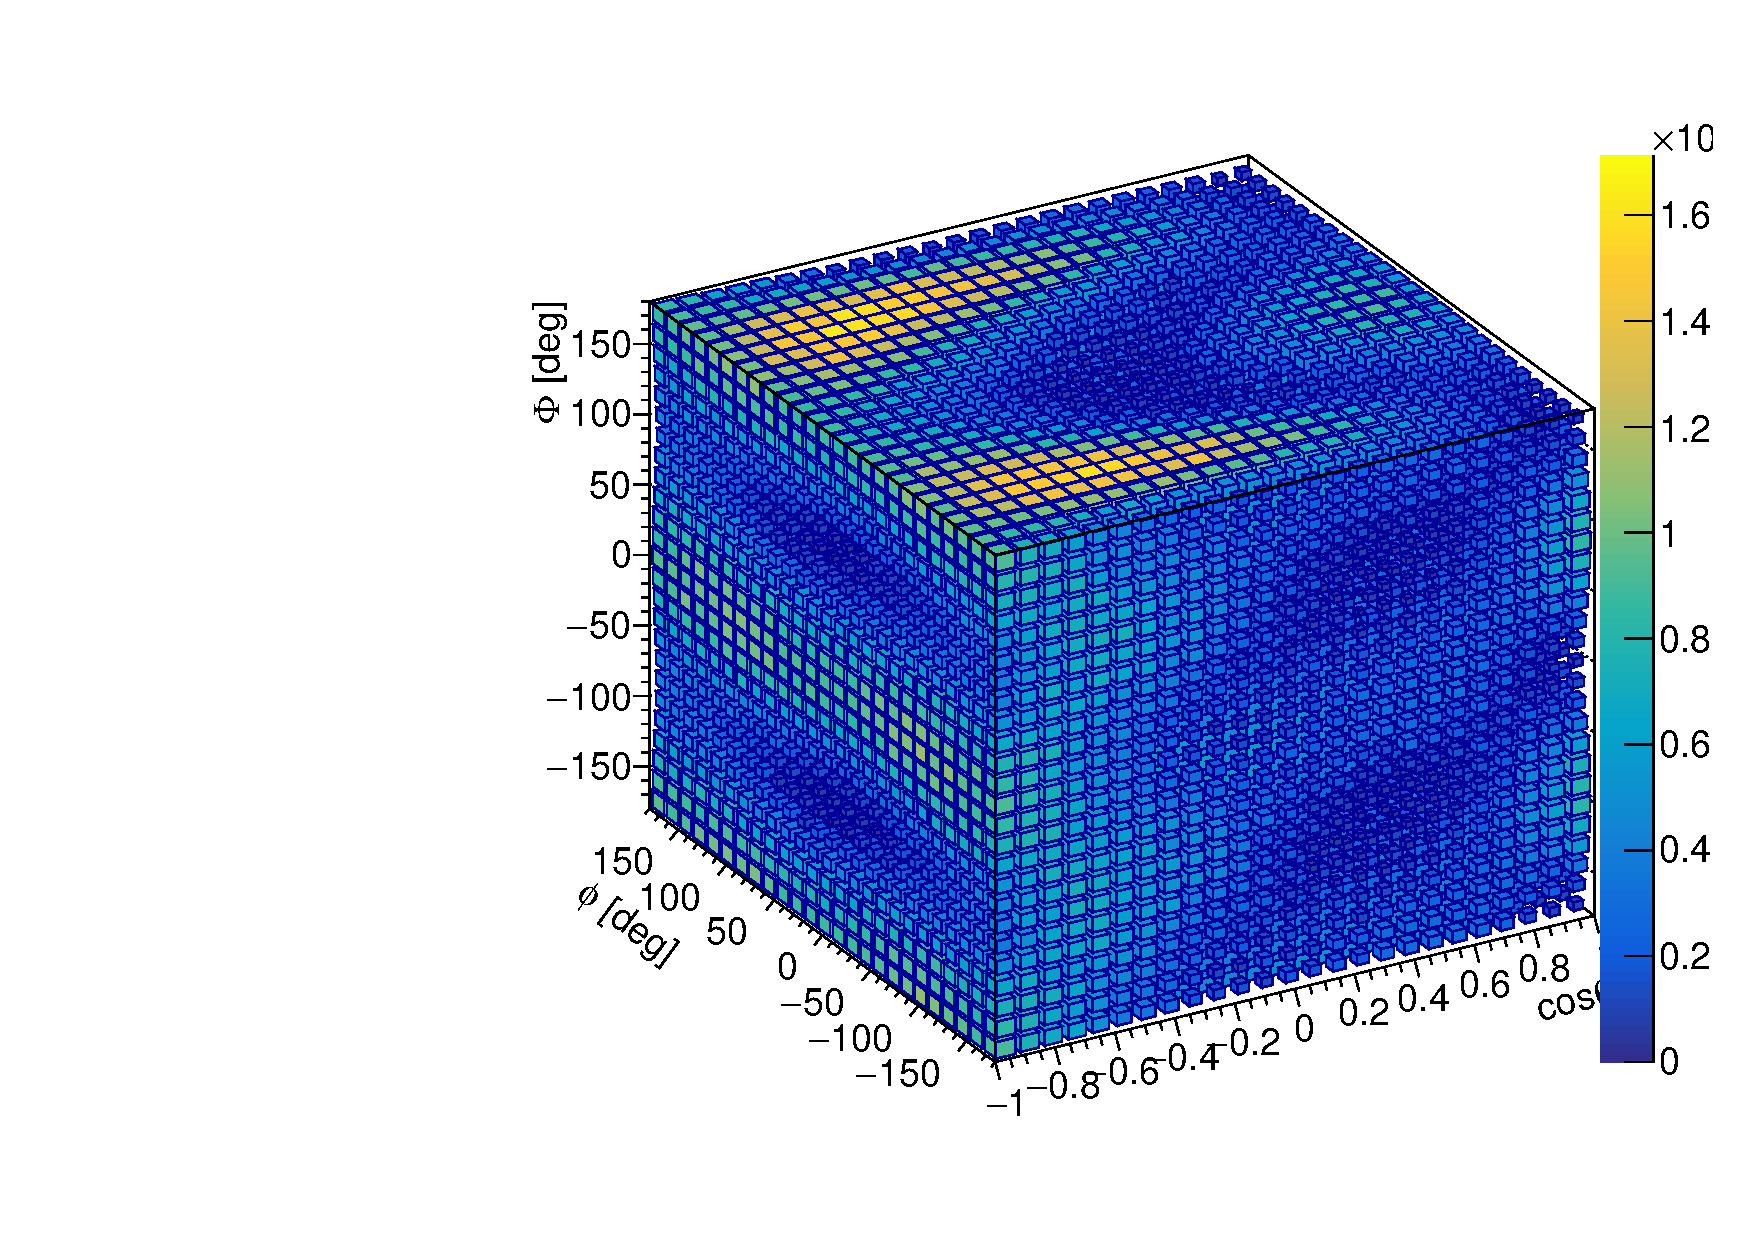
\includegraphics[width=0.5\textwidth]{photoprod_weighted/no_acc_10M/dataSbSubtr}%
  \caption{Signal sample with $N_\text{sub} = \num{9974322.5}$ events
  obtained from \cref{fig:photoprod_study_weighted_data_10M} by
  applying sideband subtraction using the discriminatory variable in
  \cref{fig:photoprod_study_weighted_discr_var_10M}.  Compare to
  \cref{fig:photoprod_study_weighted_intensity_sig}.}%
  \label{fig:photoprod_study_weighted_data_sb_subtr_10M}%
\end{figure}

For the moment analysis, we weight the intensity distributions of the
signal and the background component with the hypothetical detection
efficiency in \cref{eq:photoprod_study_acc1}, which is shown in
\cref{fig:photoprod_study_efficiency}.  From each of these weighted
intensity distributions (see
\cref{fig:photoprod_study_weighted_intensity_sig_acc,fig:photoprod_study_weighted_intensity_bkg_acc}),
we randomly draw a sample of \num{1000}~events.  The distribution of
the total sample in the discriminatory variable is shown in
\cref{fig:photoprod_study_weighted_discr_var}, the corresponding
angular distribution in \cref{fig:photoprod_study_weighted_data}.  The
sample is used to calculate the values of the measured
moments~$\hat{\vect{H}}_\text{meas}$ using
\cref{eq:photoprod_moments_meas_estimate_weighted} as well as their
augmented covariance matrix using the approach described in
\cref{fn:cov_aug_numpy}.

\begin{figure}[tbp]
  \centering%
  \subfloat[][]{%
    \label{fig:photoprod_study_weighted_intensity_sig_acc}%
    \includegraphics[width=0.5\textwidth]{photoprod_weighted/acc_1/intensitySig}%
  }%
  \subfloat[][]{%
    \label{fig:photoprod_study_weighted_intensity_bkg_acc}%
    \includegraphics[width=0.5\textwidth]{photoprod_weighted/acc_1/intensityBkg}%
  }%
  \\%
  \subfloat[][]{%
    \label{fig:photoprod_study_weighted_data}%
    \includegraphics[width=0.5\textwidth]{photoprod_weighted/acc_1/data}%
  }%
  \subfloat[][]{%
    \label{fig:photoprod_study_weighted_discr_var}%
    \includegraphics[width=0.5\textwidth]{photoprod_weighted/acc_1/hDiscrVariableSim}%
  }%
  \caption{\subfloatLabel{fig:photoprod_study_weighted_intensity_sig}~Intensity
  distribution used to generate the signal component as defined by the
  partial-wave amplitudes listed in
  \cref{tab:photoprod_study_waveset}.
  \subfloatLabel{fig:photoprod_study_weighted_intensity_bkg}~Intensity
  distribution used to generate the background component as defined by
  the partial-wave amplitudes listed in
  \cref{tab:photoprod_study_waveset_bkg}.
  \subfloatLabel{fig:photoprod_study_weighted_data_10M}~Total Monte
  Carlo data sample obtained by randomly drawing \num{e3}~events from
  each of the distributions
  in~\subfloatLabel{fig:photoprod_study_weighted_intensity_sig}
  and~\subfloatLabel{fig:photoprod_study_weighted_intensity_bkg}.
  \subfloatLabel{fig:photoprod_study_weighted_discr_var}~Distribution
  of the discriminatory variable for the total Monte Carlo data sample
  in~\subfloatLabel{fig:photoprod_study_weighted_data_10M}.  The
  shaded regions indicate the signal and side bands.}%
  \label{fig:photoprod_study_weighted_input}%
\end{figure}

Since the detection efficiency is the same as in the unweighted case,
we use the same acceptance integral matrix as in
\cref{sec:photoprod:example_unweighted} to calculate the physical
moments.
\Crefrange{fig:photoprod_study_weighted_output_H0}{fig:photoprod_study_weighted_output_H2}
show the physical moments of the signal component extracted from the
Monte Carlo data in \cref{fig:photoprod_study_weighted_data} and
compare them to the expected moment values calculated from the
partial-wave amplitudes in \cref{tab:photoprod_study_waveset} using
\crefrange{eq:photoprod_moment_0_pw_refl}{eq:photoprod_moment_2_pw_refl}.
As expected, the two sets of values  agree within statistical
uncertainties (see
\cref{fig:photoprod_study_weighted_residual_H0_re,fig:photoprod_study_weighted_residual_H1_re,fig:photoprod_study_weighted_residual_H2_im}).
Since the $H_0(L, M)$ and $H_1(L, M)$ are expected to be real-valued
and $H_2(L, M)$ to be purely imaginary (see
\cref{eq:photoprodP_moments_real_imag}), we also verify that the
imaginary parts of $H_{0, 1}(L, M)$ and the real parts of $H_2(L, M)$
are consistent with zero, which is indeed the case (see
\cref{fig:photoprod_study_weighted_comparison_H0_im,fig:photoprod_study_weighted_residual_H0_im,fig:photoprod_study_weighted_comparison_H1_im,fig:photoprod_study_weighted_residual_H1_im,fig:photoprod_study_weighted_comparison_H2_re,fig:photoprod_study_weighted_residual_H2_re}).

\begin{figure}[tbp]
  \centering%
  \subfloat[][]{%
    \label{fig:photoprod_study_weighted_comparison_H0_re}%
    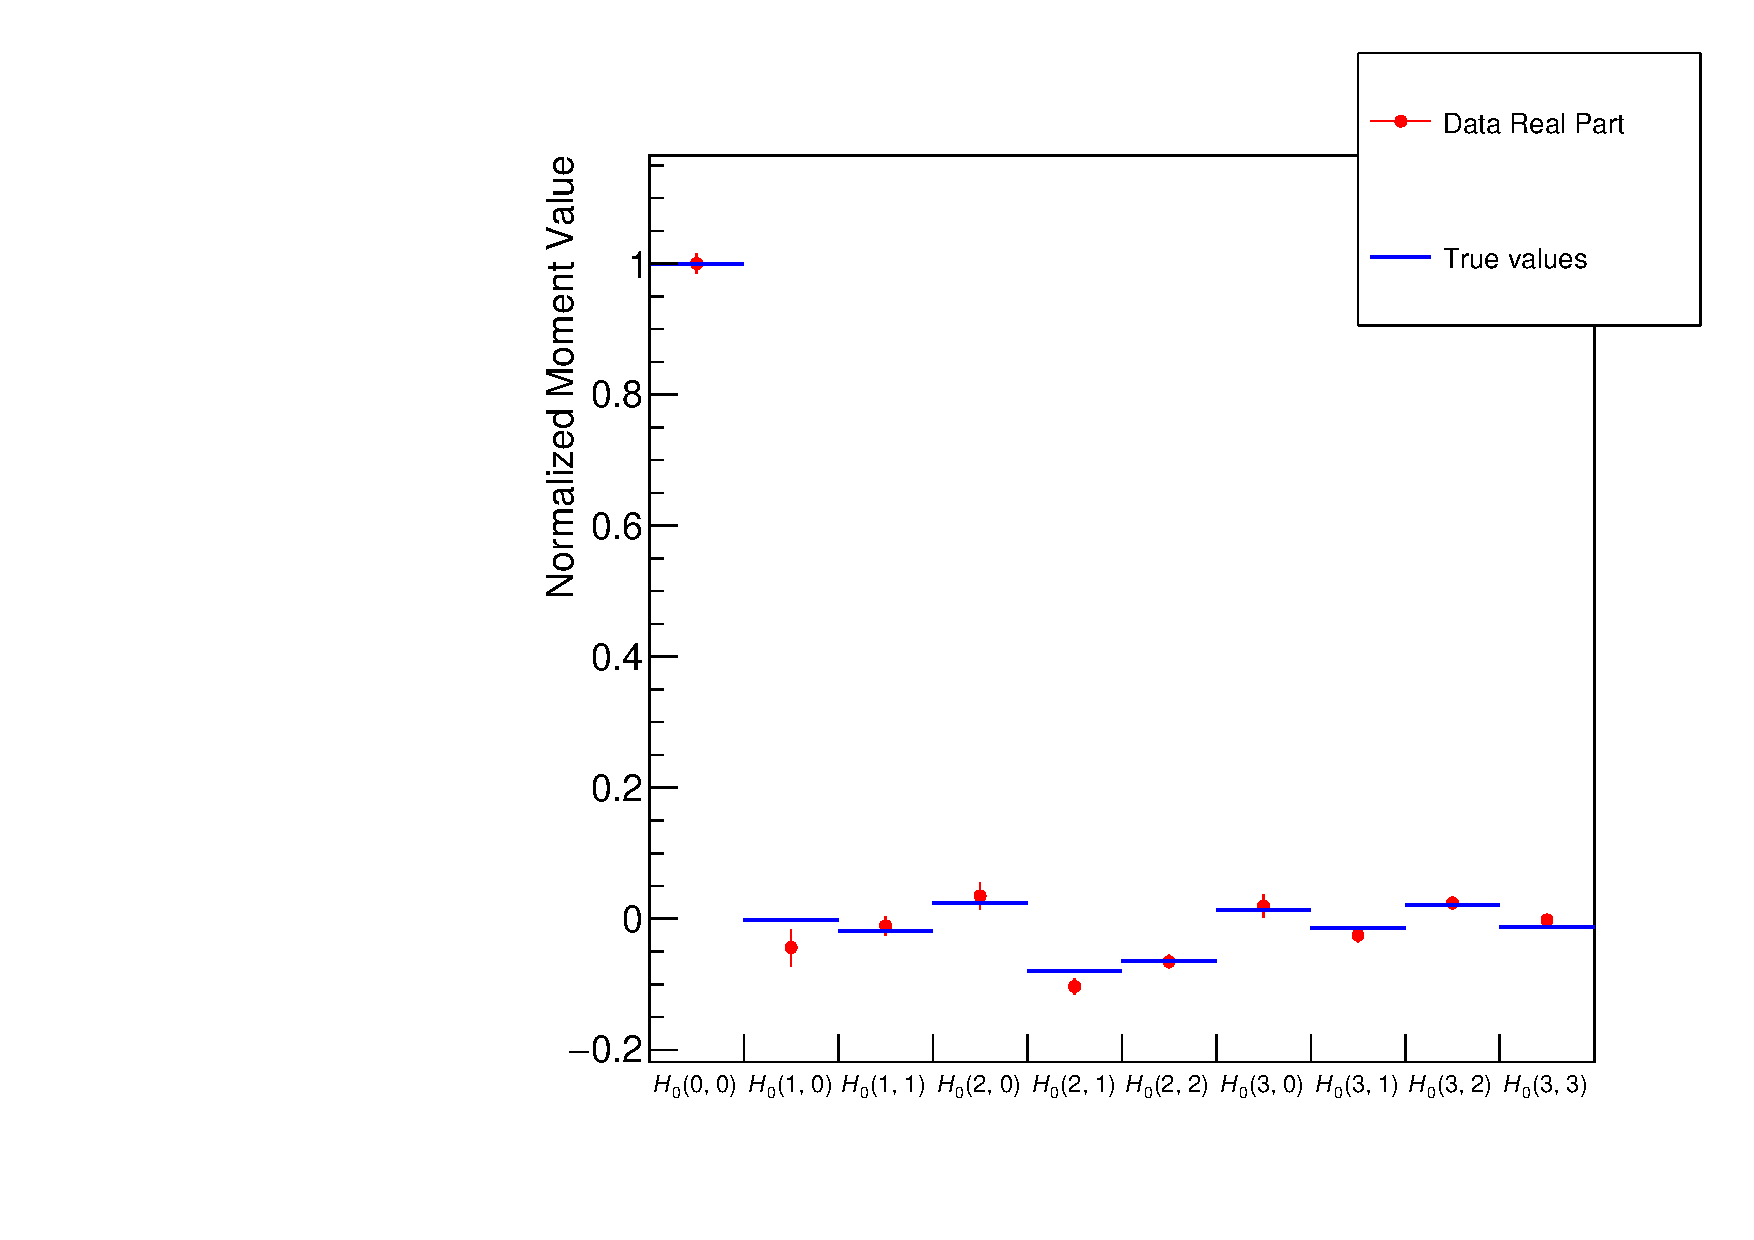
\includegraphics[width=0.5\textwidth]{photoprod_weighted/acc_1/hmass_1.50_Compare_H0_Re}%
  }%
  \subfloat[][]{%
    \label{fig:photoprod_study_weighted_comparison_H0_im}%
    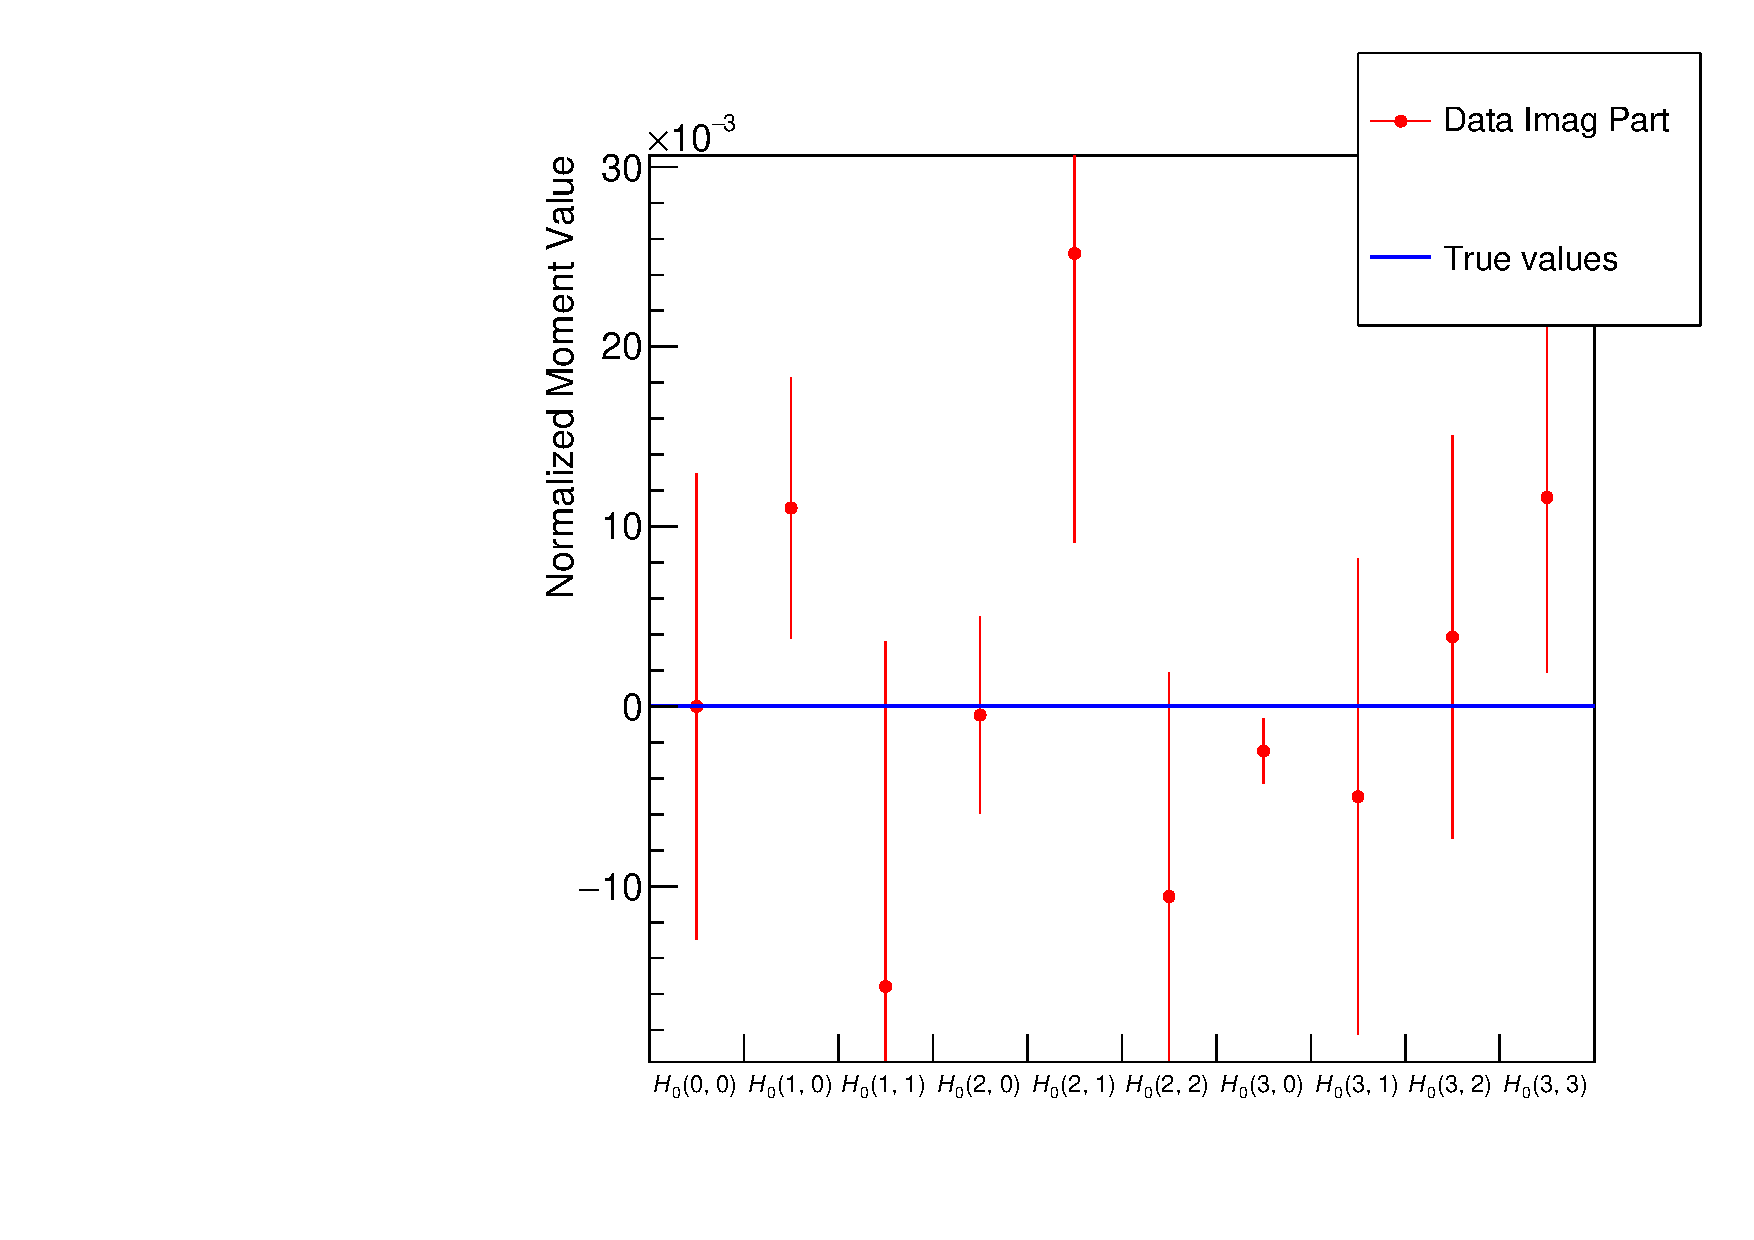
\includegraphics[width=0.5\textwidth]{photoprod_weighted/acc_1/hmass_1.50_Compare_H0_Im}%
  }%
  \\%
  \subfloat[][]{%
    \label{fig:photoprod_study_weighted_residual_H0_re}%
    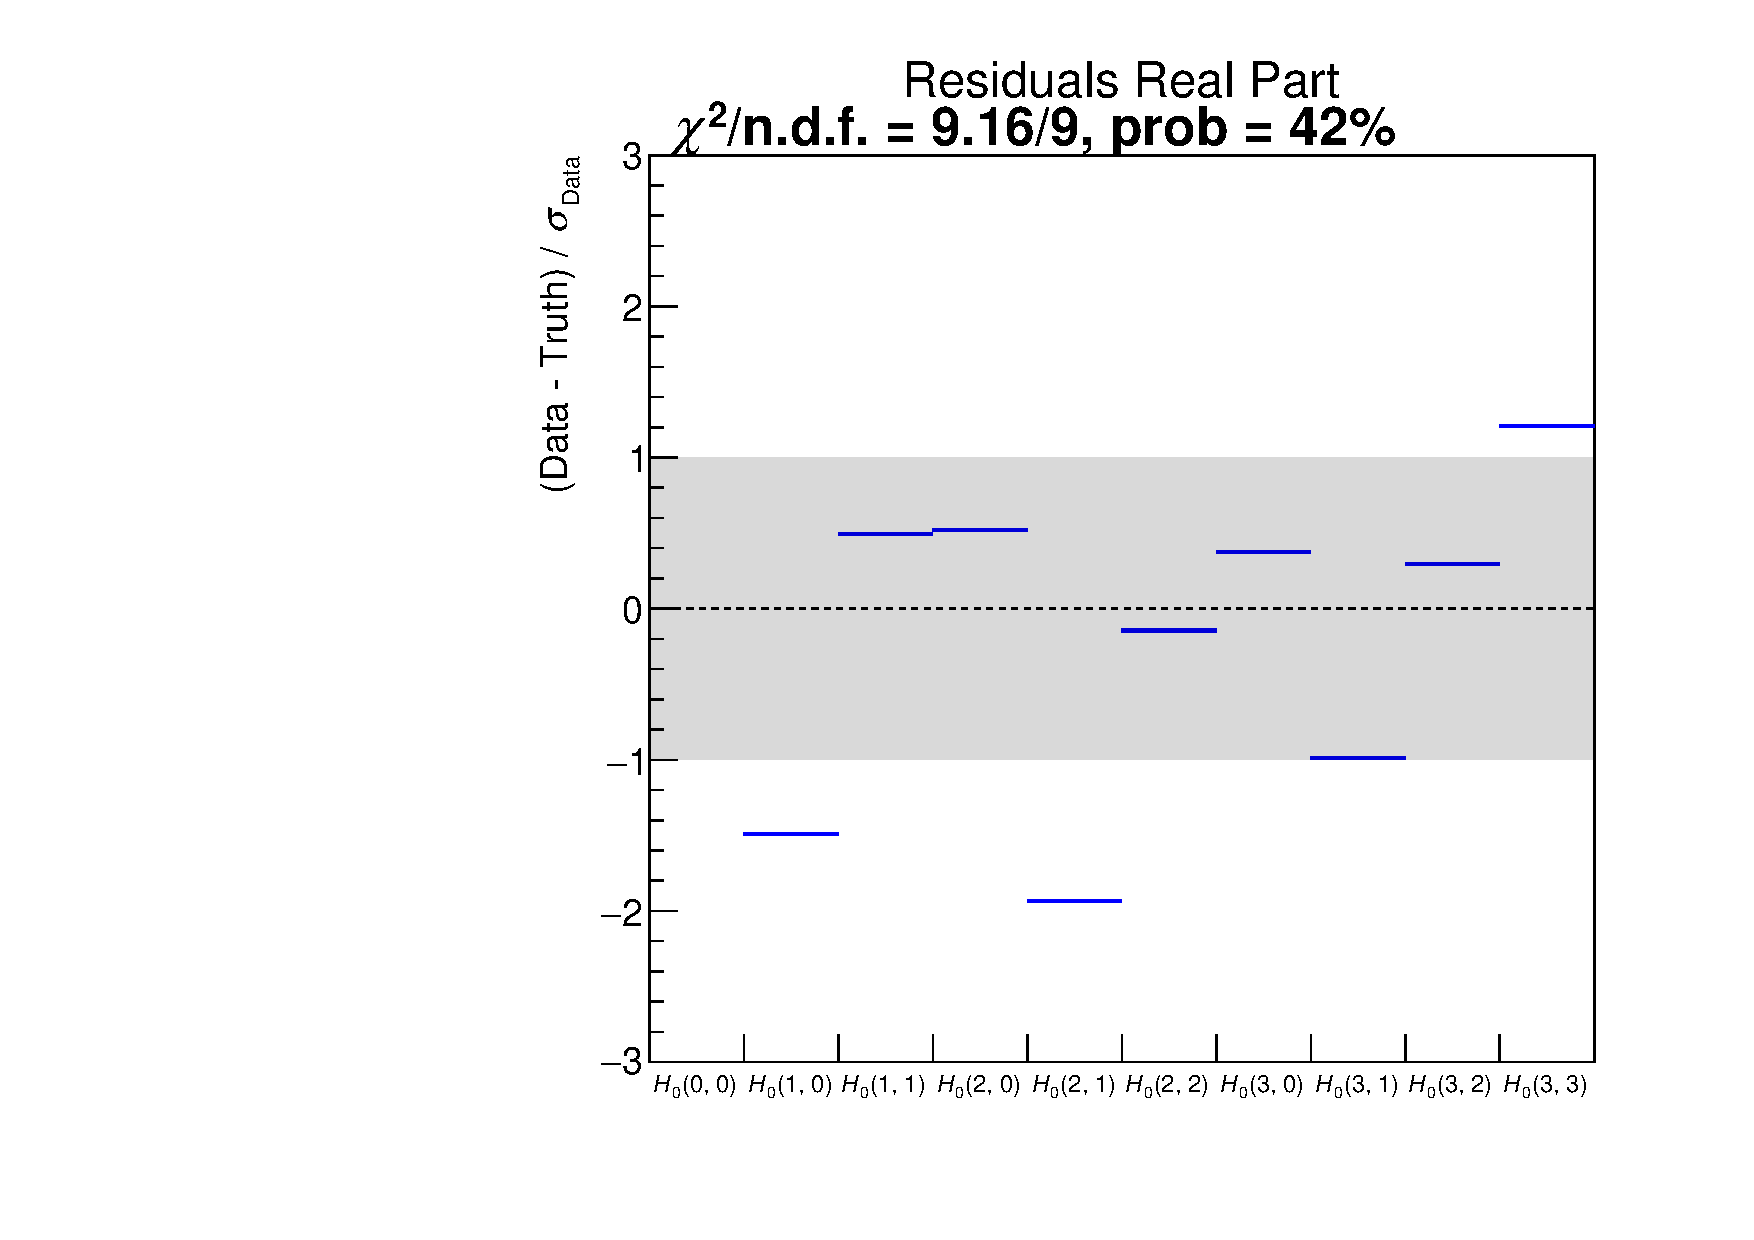
\includegraphics[width=0.5\textwidth]{photoprod_weighted/acc_1/hmass_1.50_Residuals_H0_Re}%
  }%
  \subfloat[][]{%
    \label{fig:photoprod_study_weighted_residual_H0_im}%
    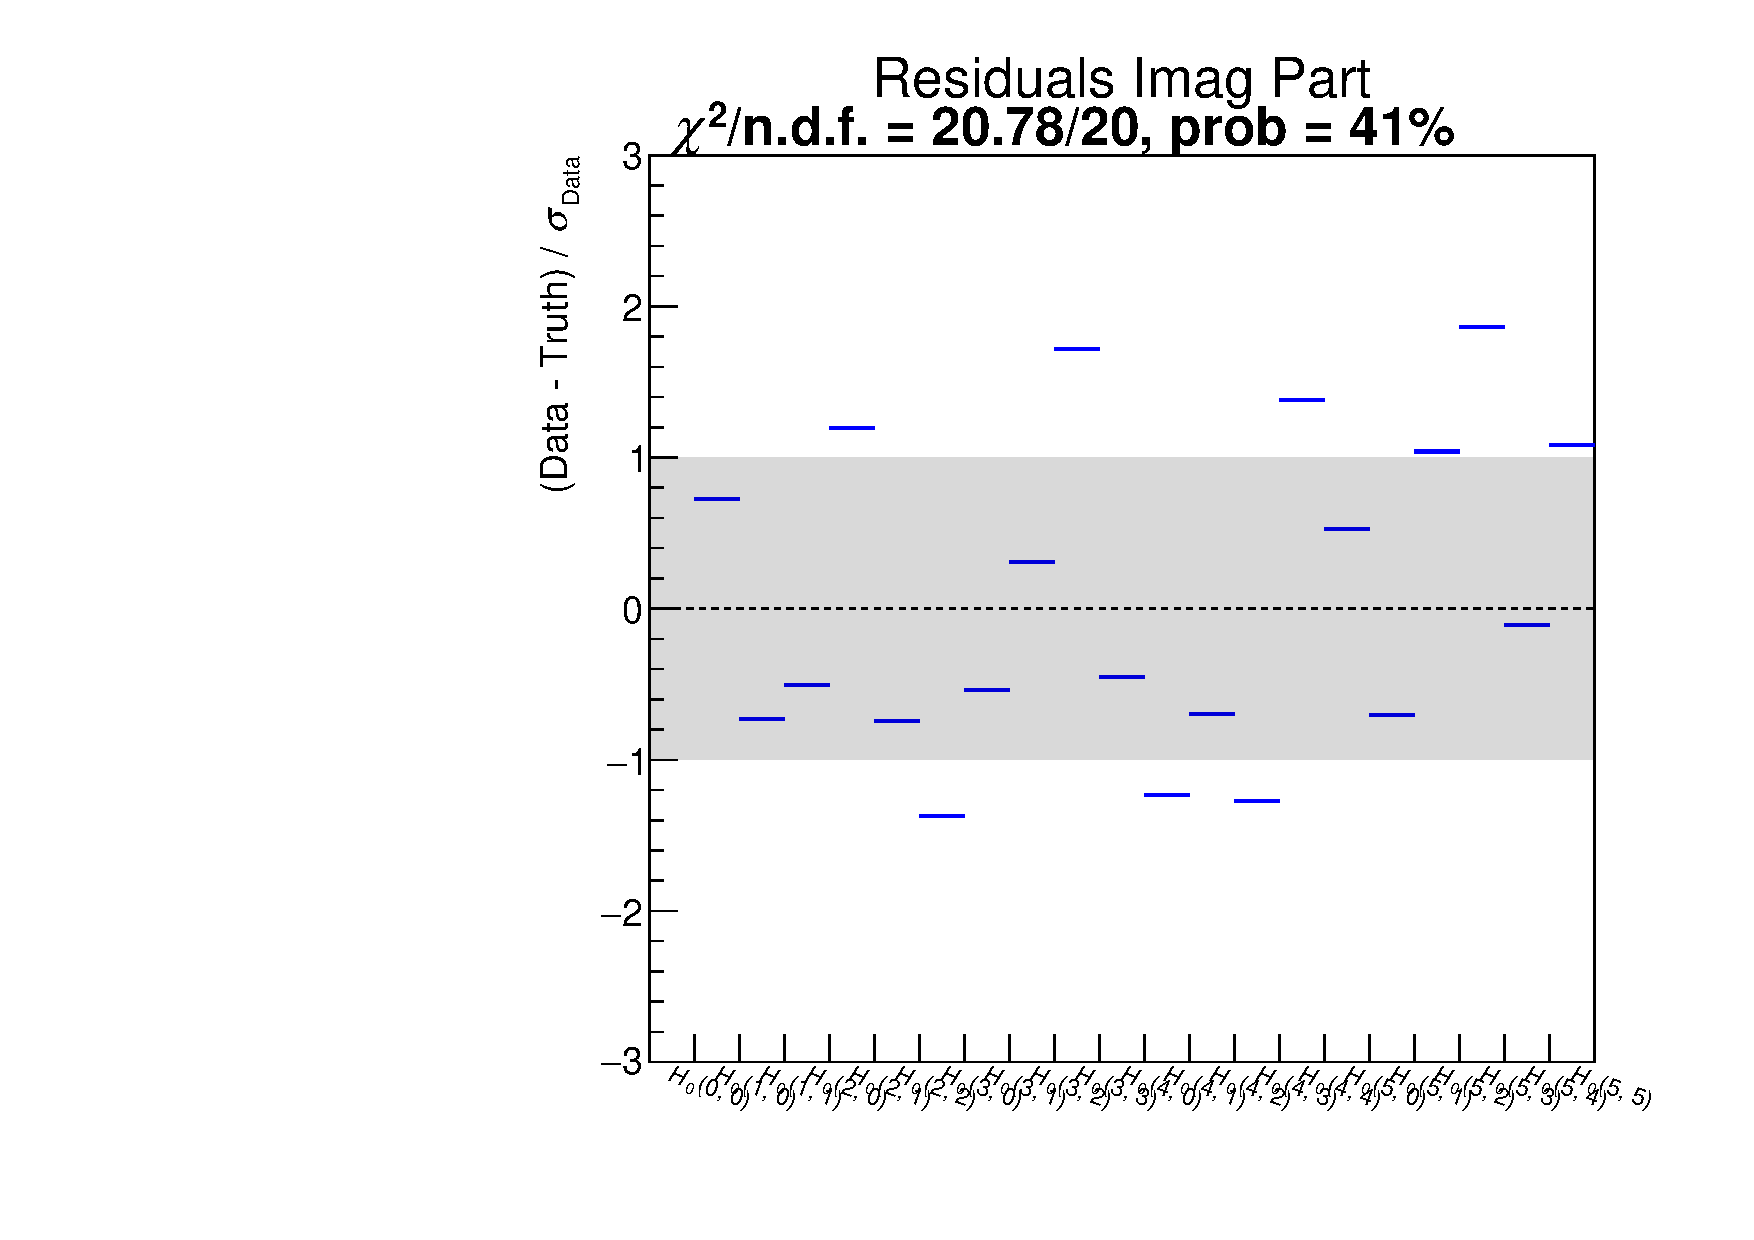
\includegraphics[width=0.5\textwidth]{photoprod_weighted/acc_1/hmass_1.50_Residuals_H0_Im}%
  }%
  \caption{Upper row: Comparison of the physical moments $H_0(L, M)$
  (red points with uncertainties) extracted from the
  sideband-subtracted Monte Carlo data, which are generated using the
  partial-wave amplitudes in
  \cref{tab:photoprod_study_waveset,tab:photoprod_study_waveset_bkg}
  and the detection efficiency in \cref{eq:photoprod_study_acc1}, with
  the expected values (blue lines).  Both sets of values are
  normalized to the value of $H_0(0, 0)$ in the respective set.
  \subfloatLabel{fig:photoprod_study_comparison_H0_re}~shows the real
  part of $H_0(L, M)$,
  \subfloatLabel{fig:photoprod_study_comparison_H0_im}~the imaginary
  part.  Note that moments with $L > 4$ are expected to be zero due to
  the chosen wave set.  Lower row: corresponding residuals.}%
  \label{fig:photoprod_study_weighted_output_H0}%
\end{figure}

\begin{figure}[tbp]
  \centering%
  \subfloat[][]{%
    \label{fig:photoprod_study_weighted_comparison_H1_re}%
    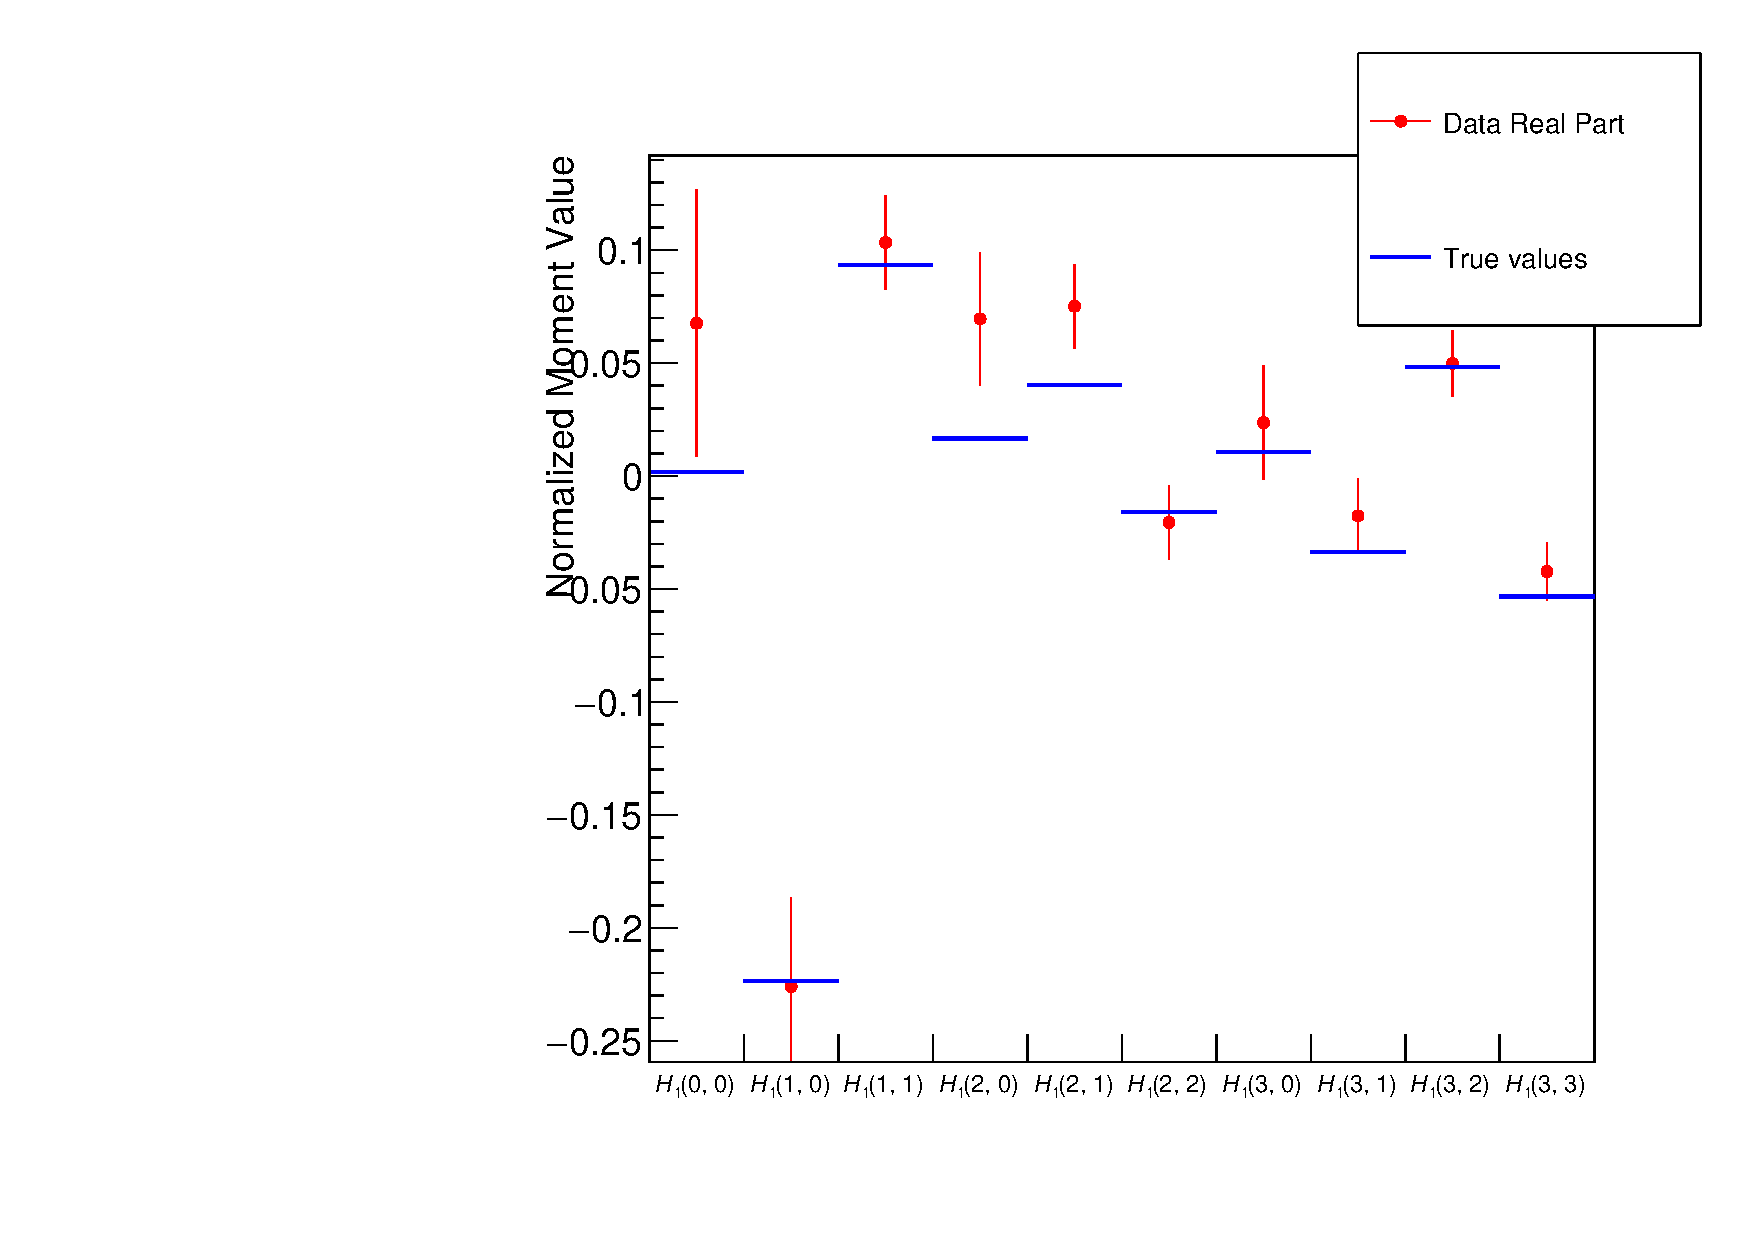
\includegraphics[width=0.5\textwidth]{photoprod_weighted/acc_1/hmass_1.50_Compare_H1_Re}%
  }%
  \subfloat[][]{%
    \label{fig:photoprod_study_weighted_comparison_H1_im}%
    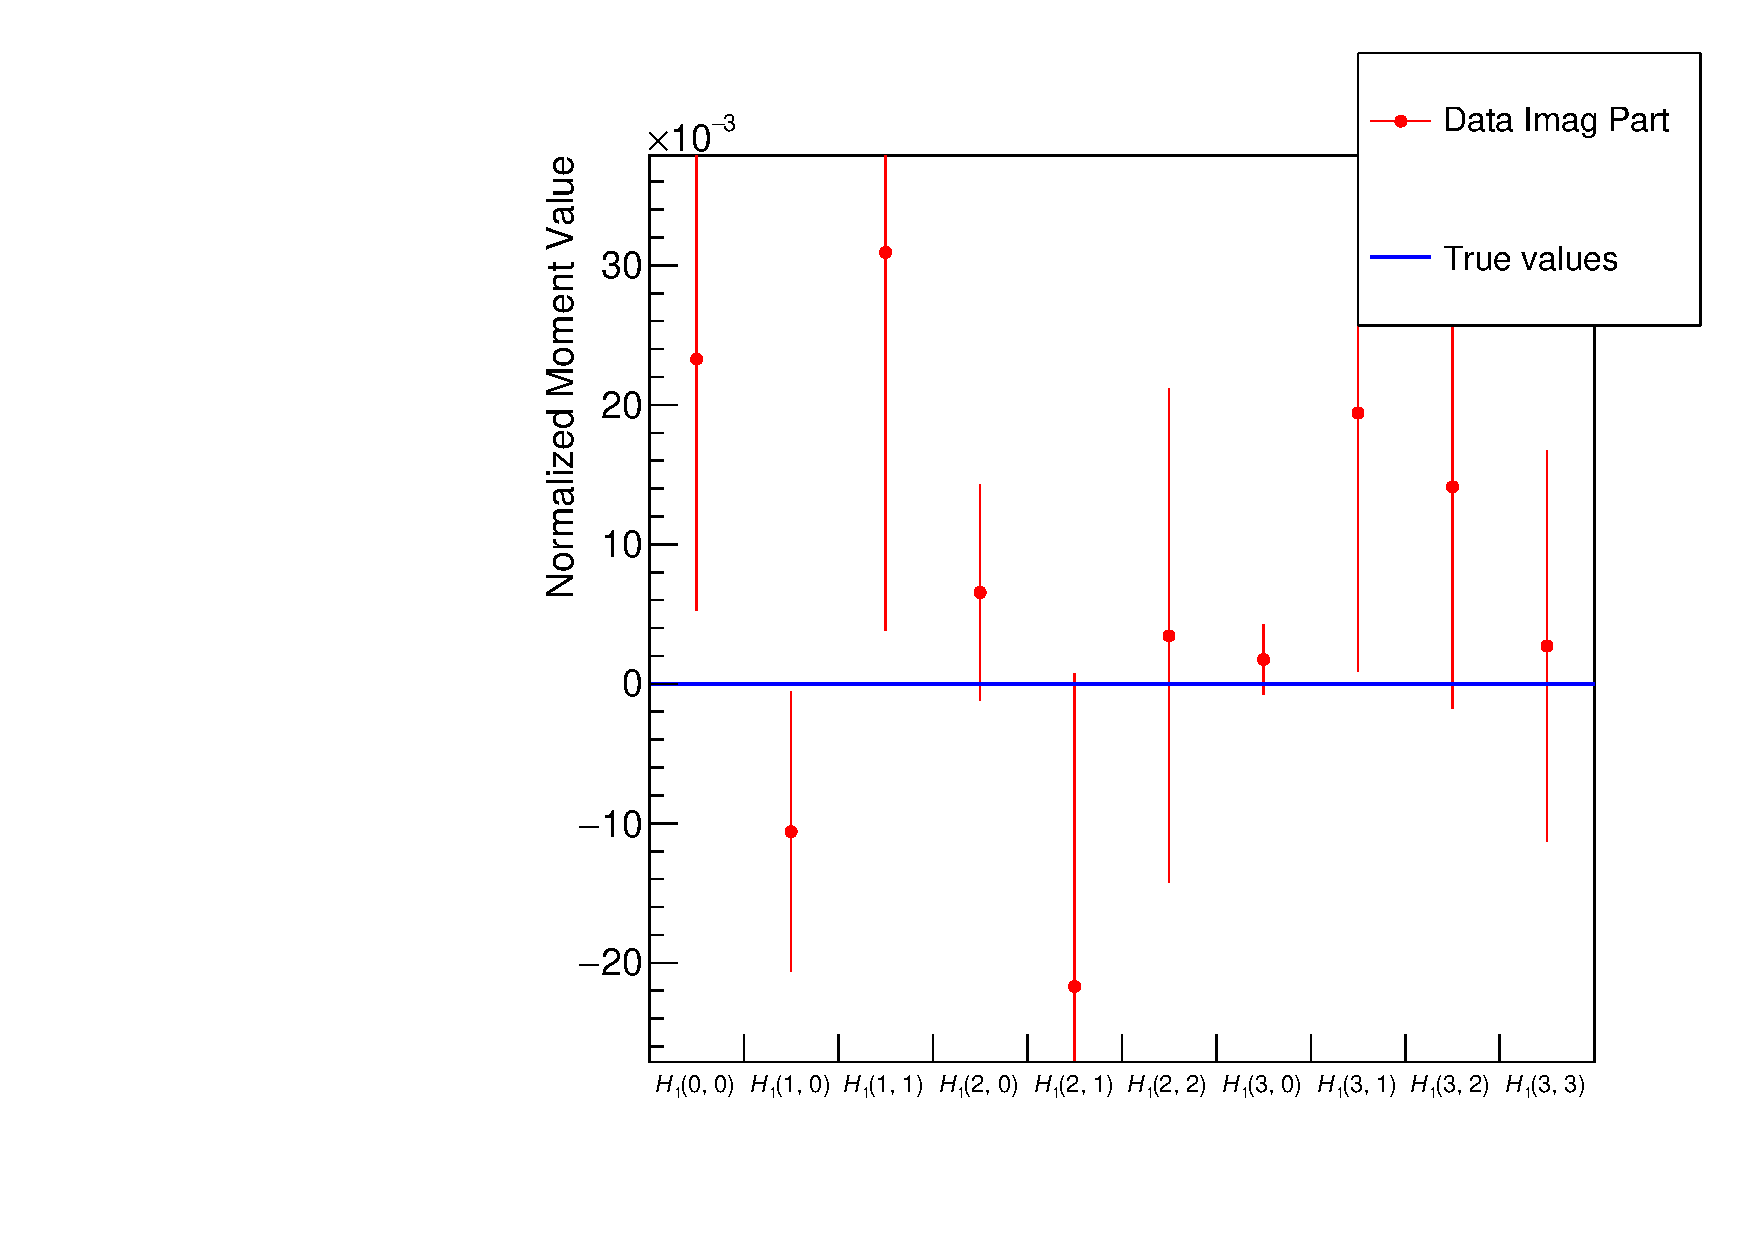
\includegraphics[width=0.5\textwidth]{photoprod_weighted/acc_1/hmass_1.50_Compare_H1_Im}%
  }%
  \\%
  \subfloat[][]{%
    \label{fig:photoprod_study_weighted_residual_H1_re}%
    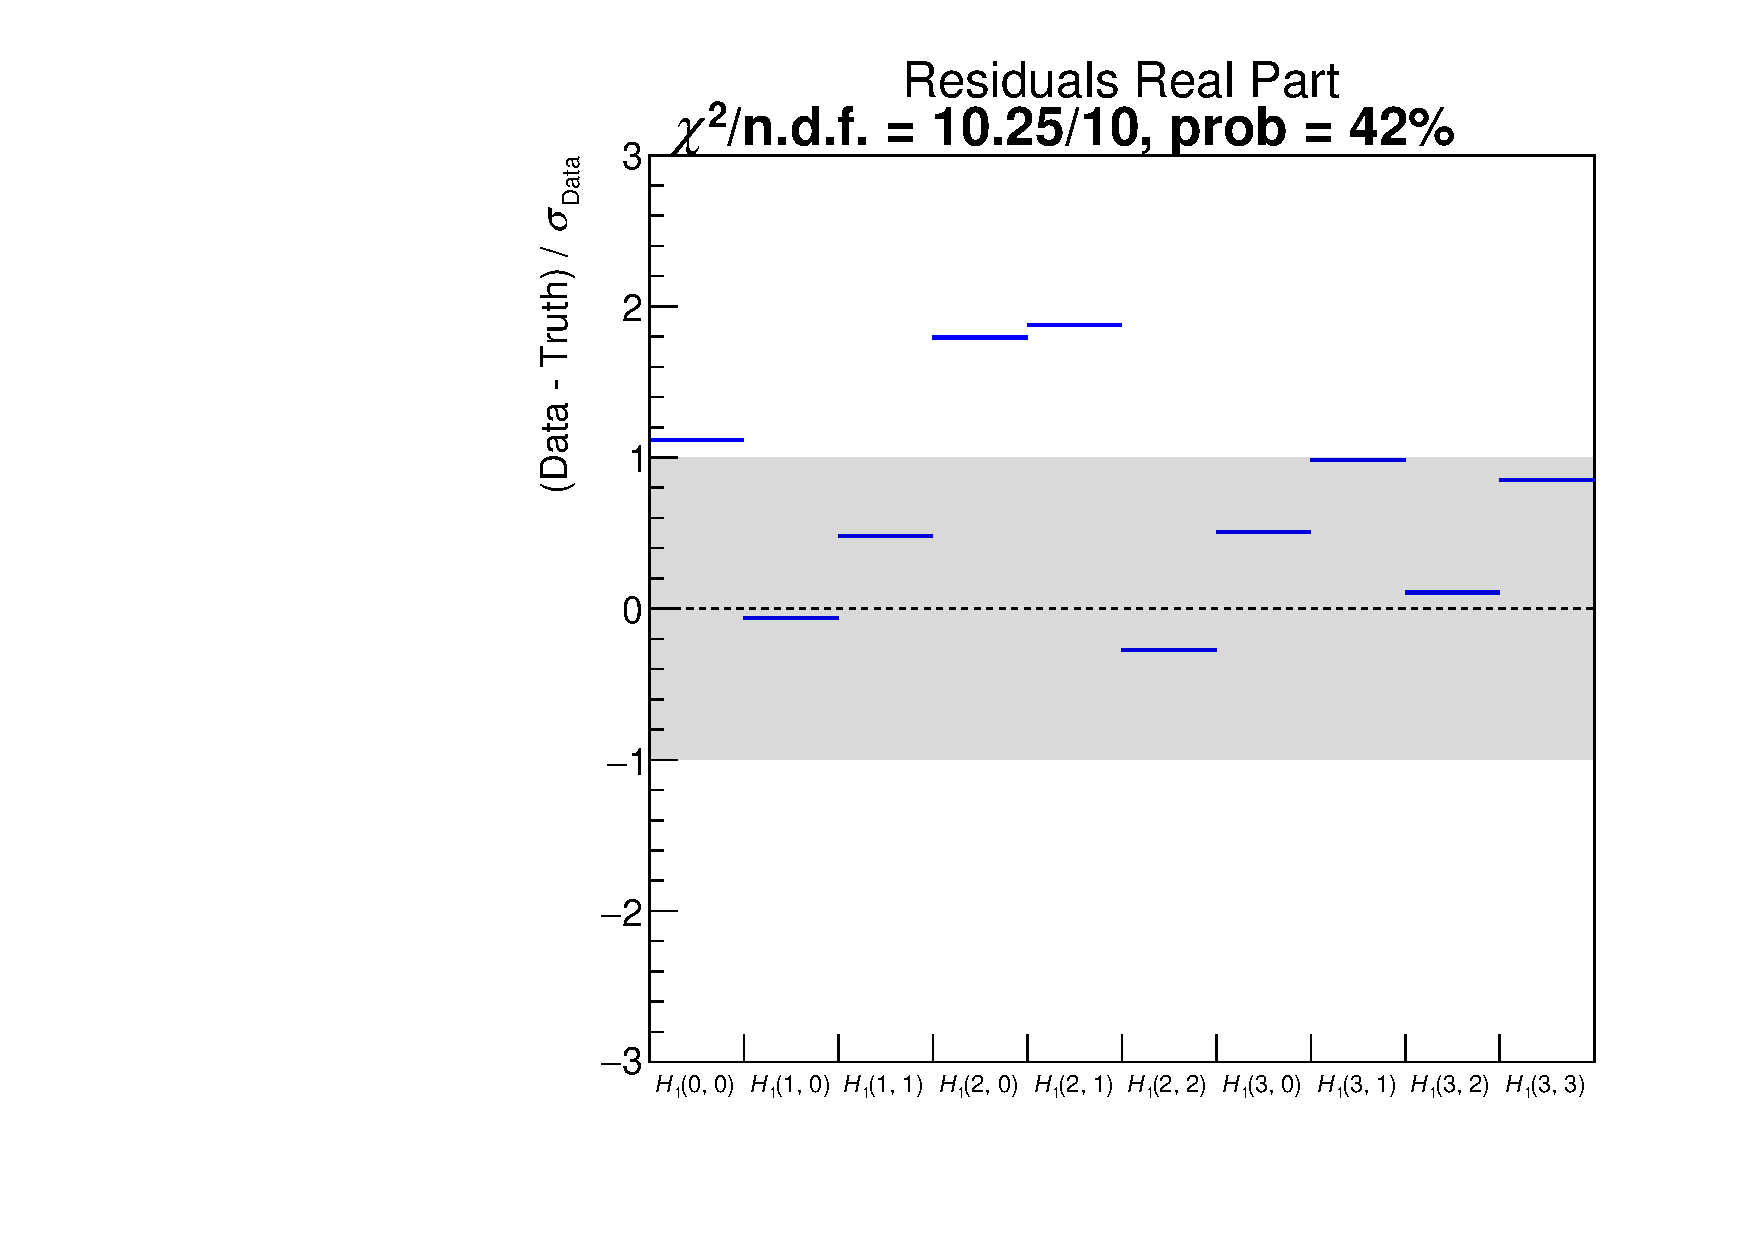
\includegraphics[width=0.5\textwidth]{photoprod_weighted/acc_1/hmass_1.50_Residuals_H1_Re}%
  }%
  \subfloat[][]{%
    \label{fig:photoprod_study_weighted_residual_H1_im}%
    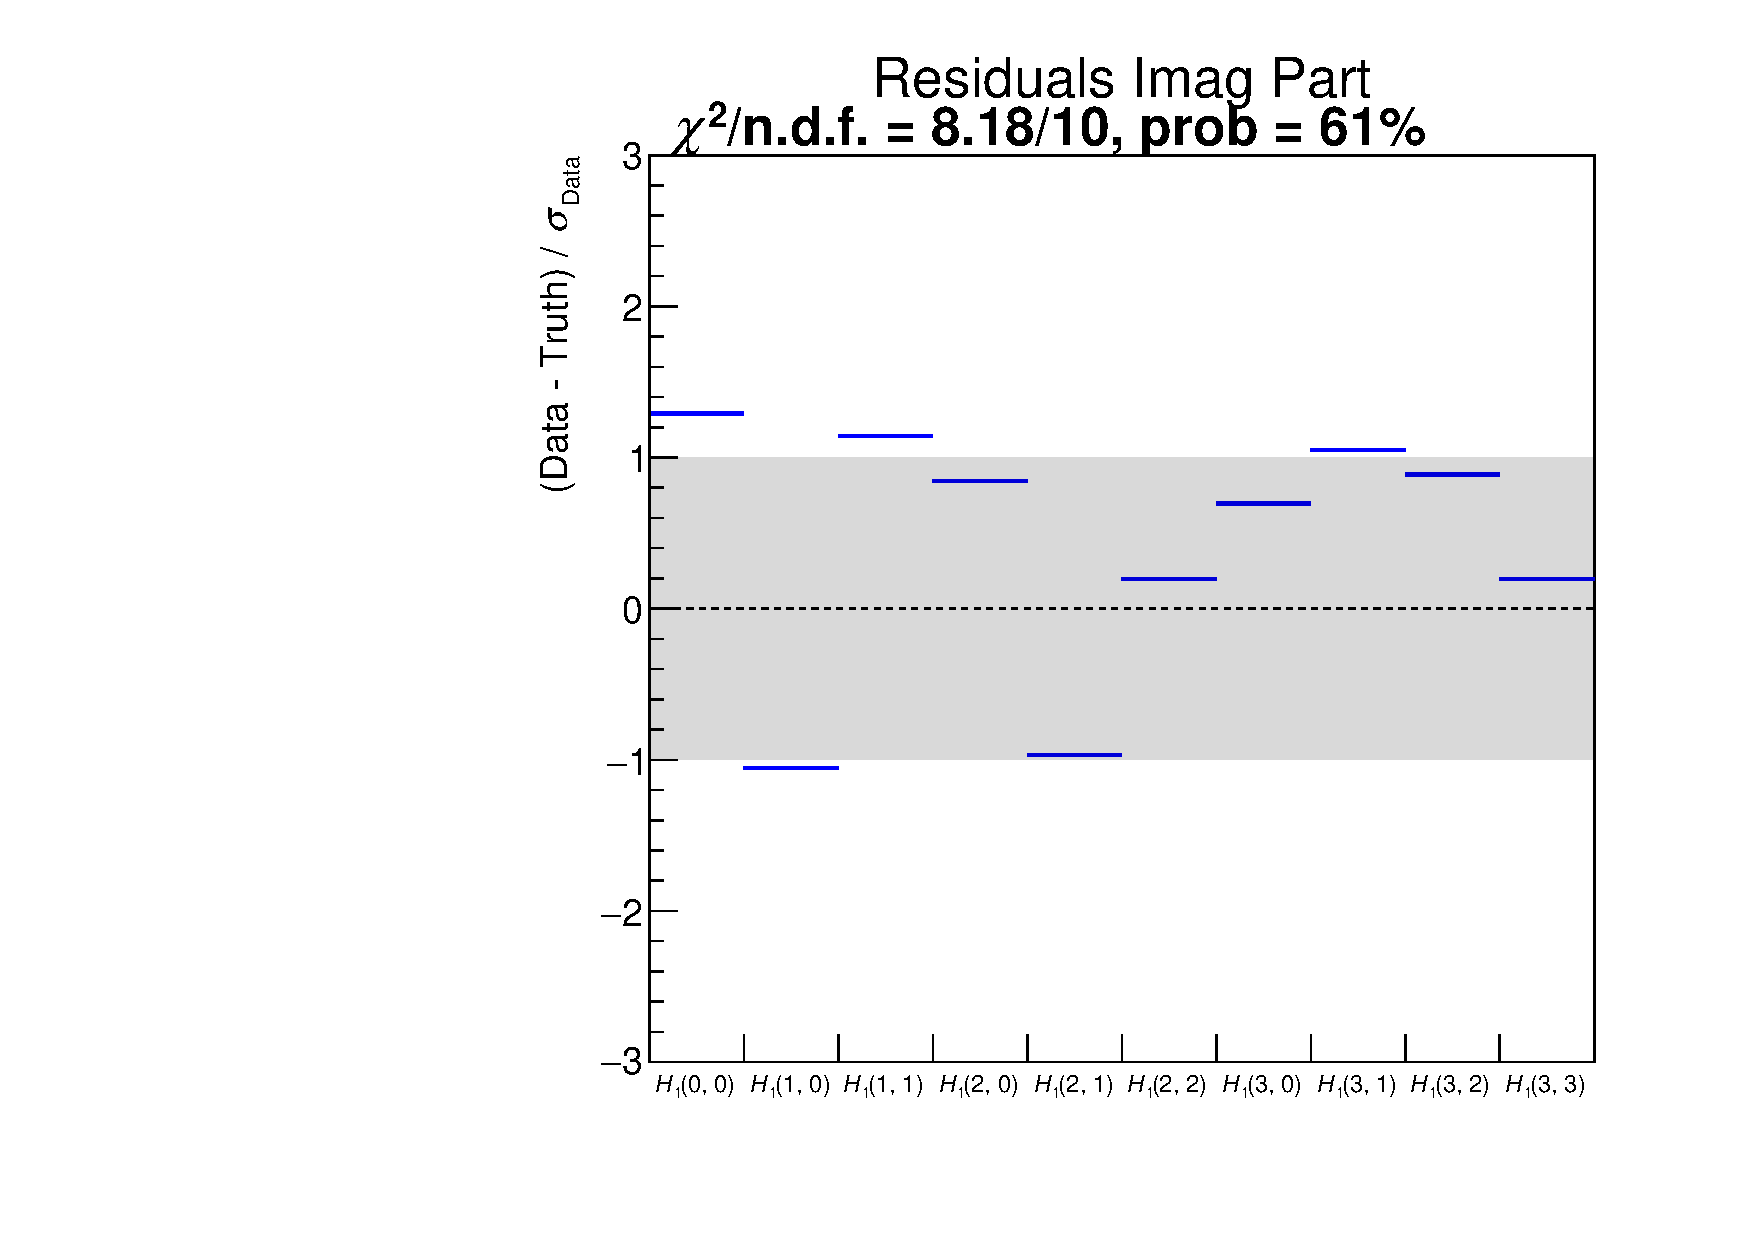
\includegraphics[width=0.5\textwidth]{photoprod_weighted/acc_1/hmass_1.50_Residuals_H1_Im}%
  }%
  \caption{Same as \cref{fig:photoprod_study_weighted_output_H0} but
  for $H_1(L, M)$.}%
  \label{fig:photoprod_study_weighted_output_H1}%
\end{figure}

\begin{figure}[tbp]
  \centering%
  \subfloat[][]{%
    \label{fig:photoprod_study_weighted_comparison_H2_re}%
    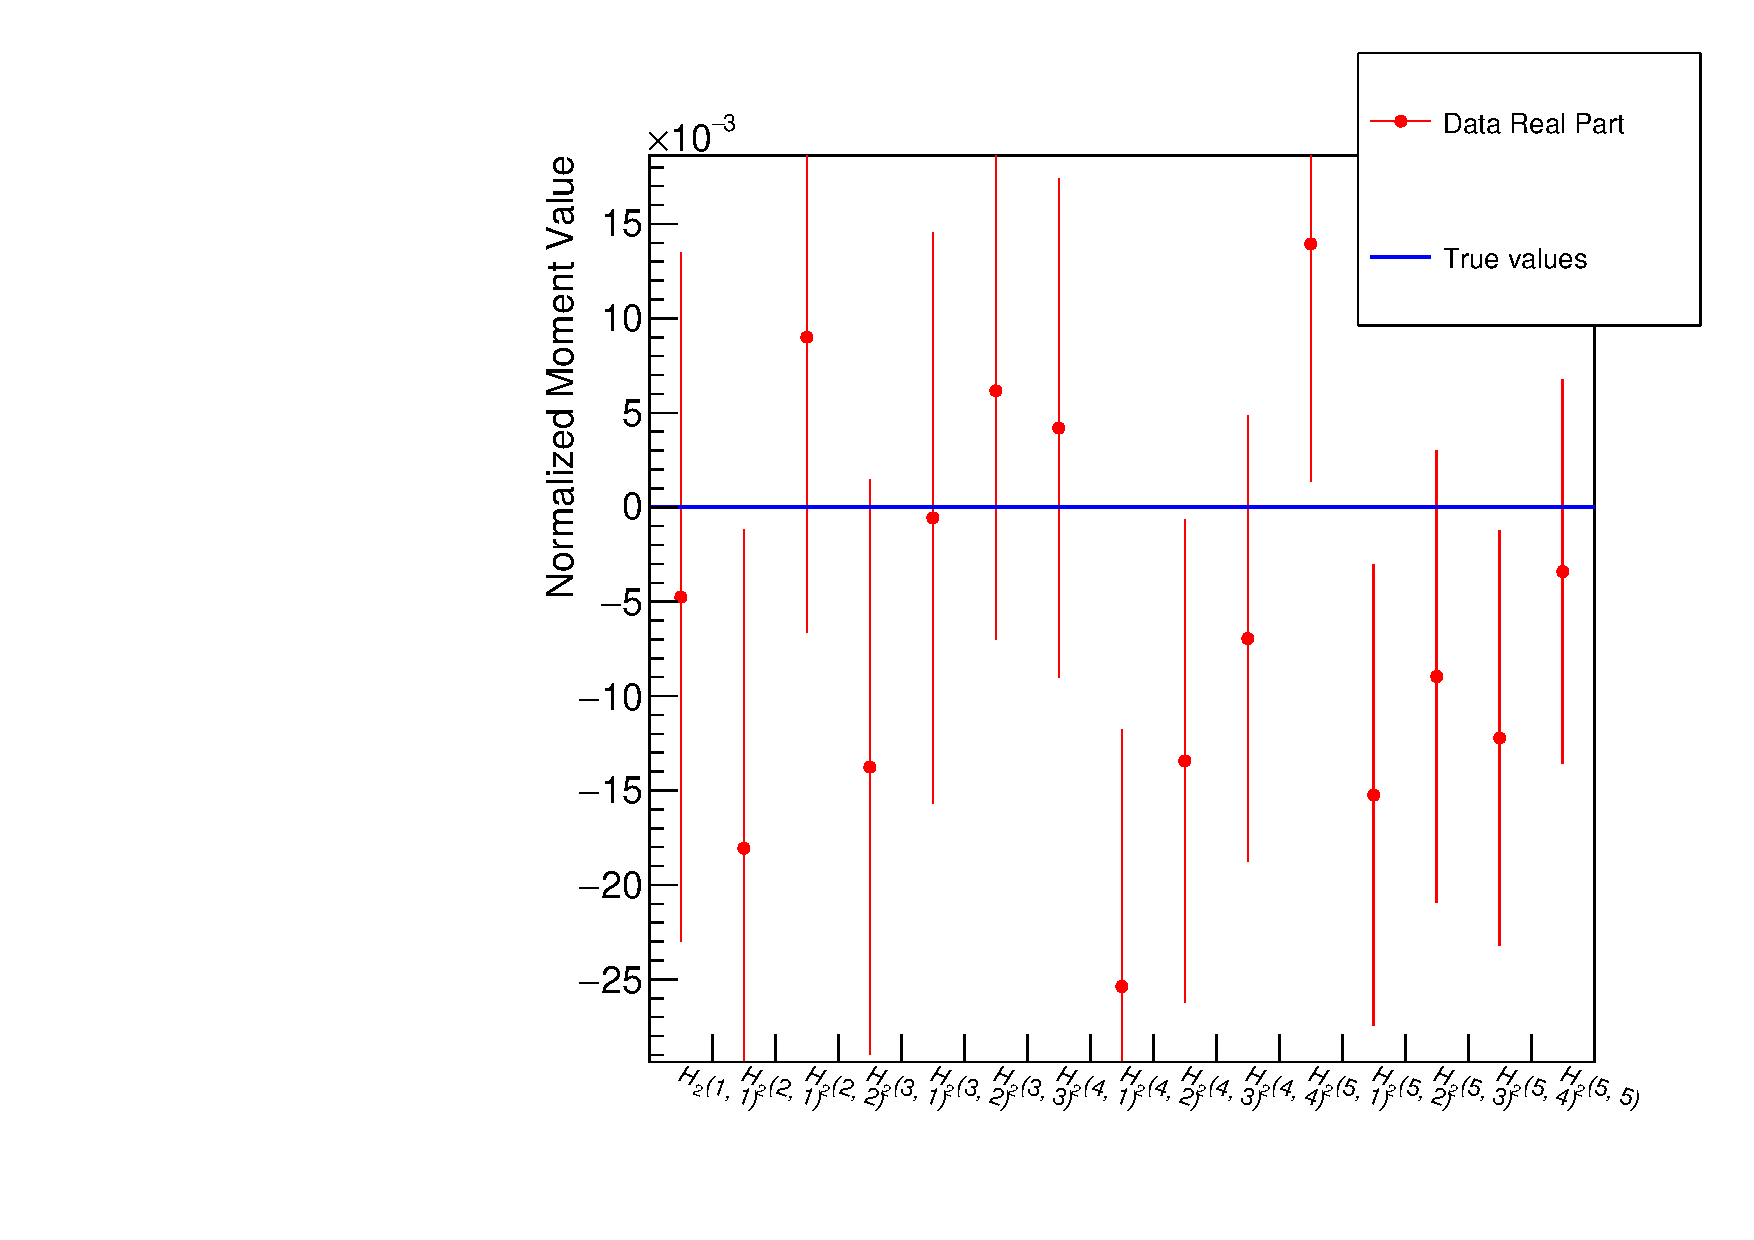
\includegraphics[width=0.5\textwidth]{photoprod_weighted/acc_1/hmass_1.50_Compare_H2_Re}%
  }%
  \subfloat[][]{%
    \label{fig:photoprod_study_weighted_comparison_H2_im}%
    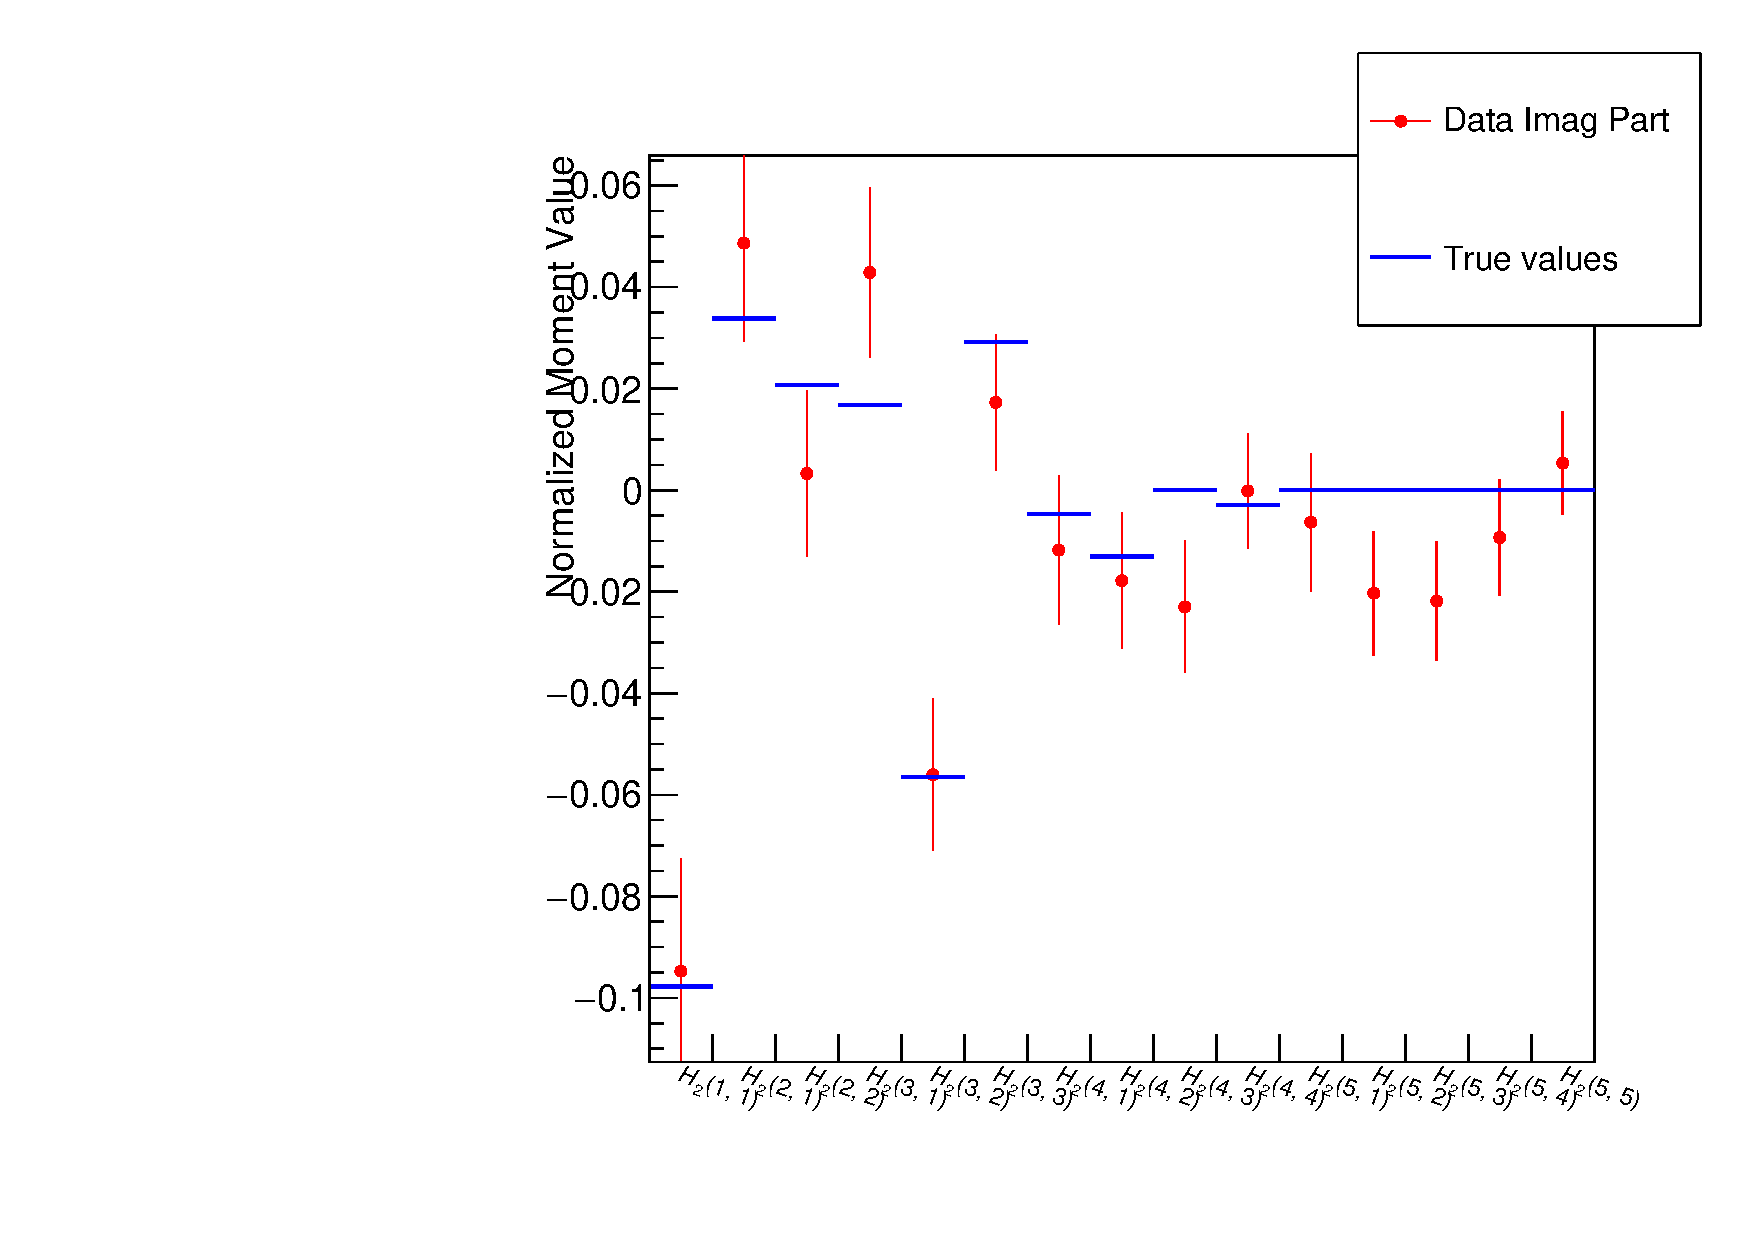
\includegraphics[width=0.5\textwidth]{photoprod_weighted/acc_1/hmass_1.50_Compare_H2_Im}%
  }%
  \\%
  \subfloat[][]{%
    \label{fig:photoprod_study_weighted_residual_H2_re}%
    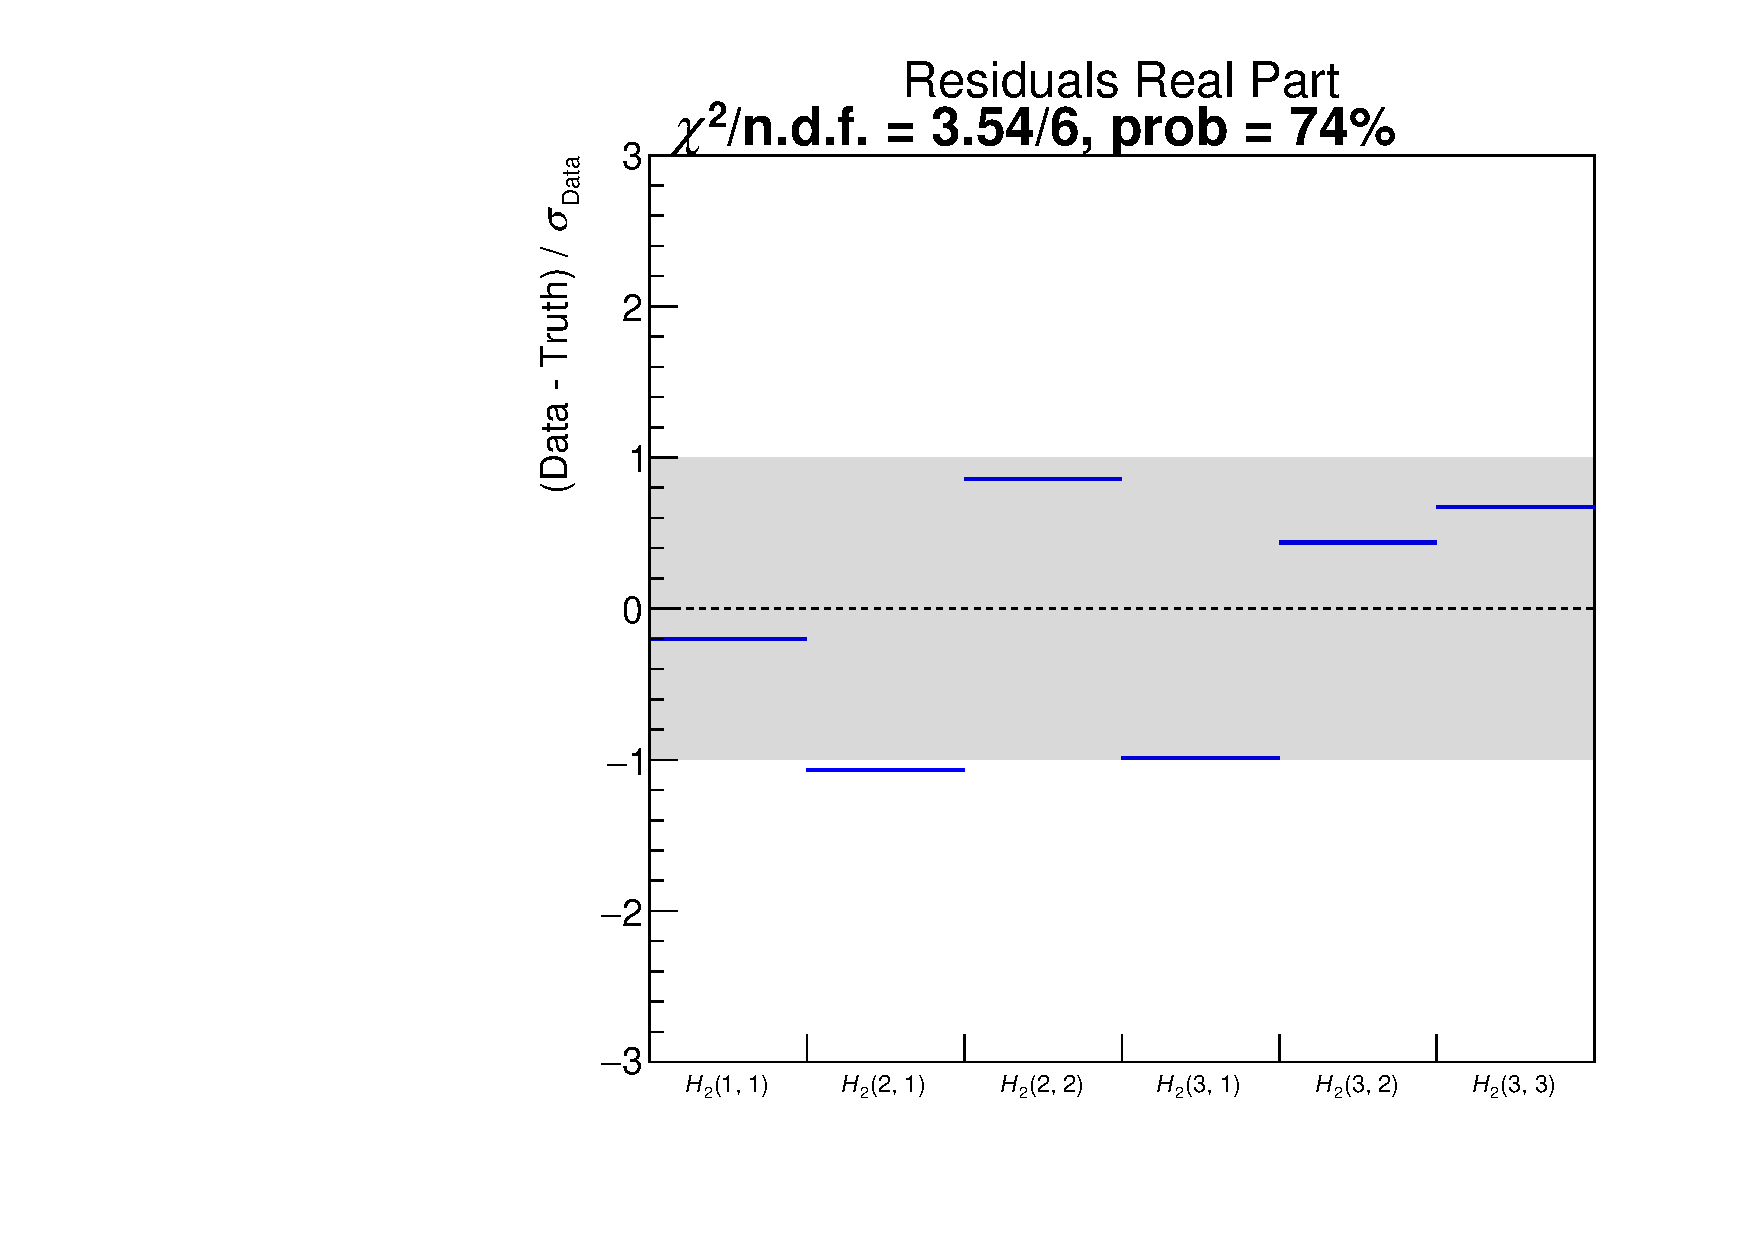
\includegraphics[width=0.5\textwidth]{photoprod_weighted/acc_1/hmass_1.50_Residuals_H2_Re}%
  }%
  \subfloat[][]{%
    \label{fig:photoprod_study_weighted_residual_H2_im}%
    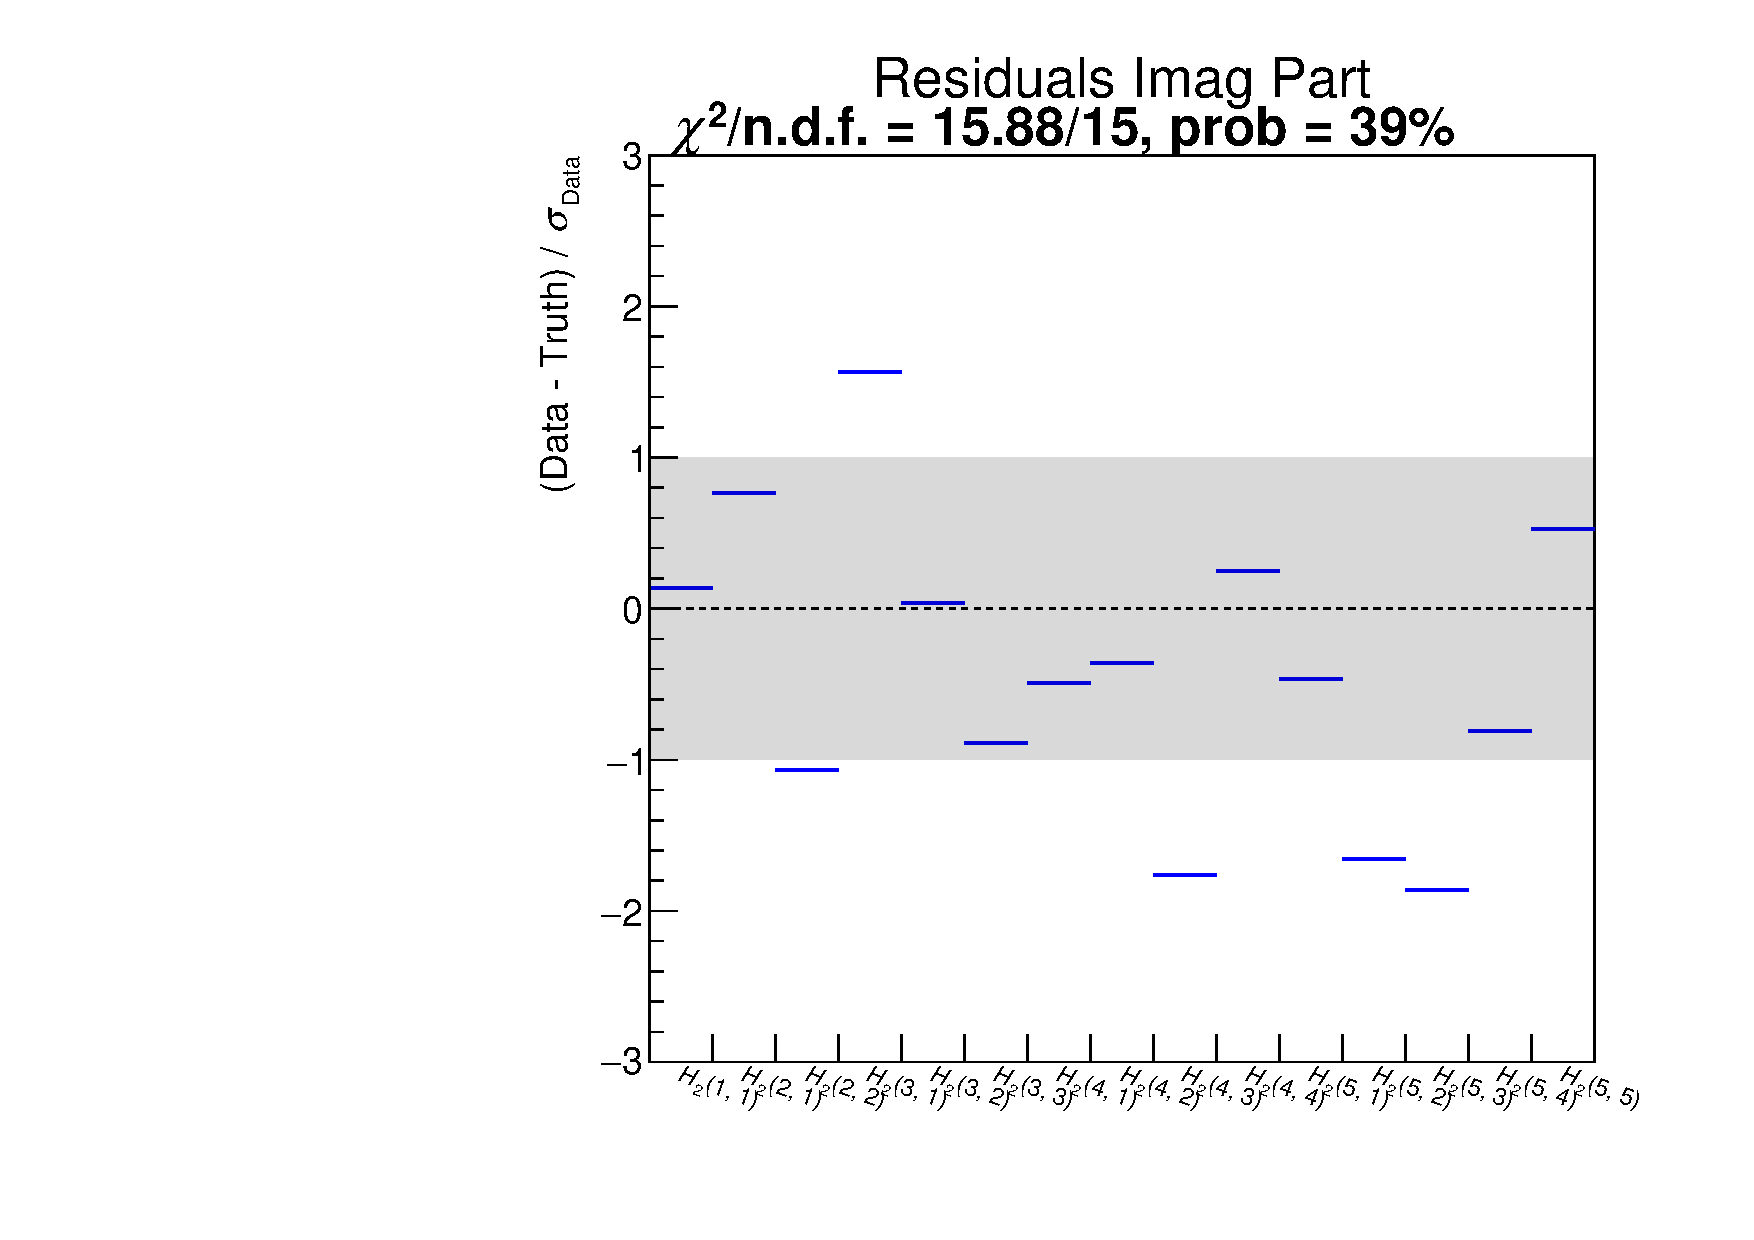
\includegraphics[width=0.5\textwidth]{photoprod_weighted/acc_1/hmass_1.50_Residuals_H2_Im}%
  }%
  \caption{Same as \cref{fig:photoprod_study_weighted_output_H0} but
  for $H_2(L, M)$.}%
  \label{fig:photoprod_study_weighted_output_H2}%
\end{figure}


\clearpage
\subsection{Combining data samples and taking into account time dependence}%
\label{sec:photoprod:comb_data}

Up to now, we assumed that the experimental data used to
estimate~$\vect{H}_\text{meas}$ were taken using the same experimental
conditions.  However, in practice one often has several data samples
that were taken with different experimental conditions, which one
wants to combine.  This means that in general the photon-beam
polarization~$P_\gamma$, the detection efficiency $\eta(\Omega,
\Phi)$, and consequently also the acceptance integral
matrix~$\mat{I}^\text{acc}$ are functions of time.

Given $N_\text{sample}$~data samples indexed by~$j$, each of which
taken using constant experimental conditions represented
by~$\prescript{(j)}{}{P_\gamma}$ and $\prescript{(j)}{}{\eta}(\Omega,
\Phi)$, we calculate the
set~$\Set[1]{\prescript{(j)}{}{\vphantom{\vect{H}}}\hat{\vect{H}}_\text{meas}}$
and the corresponding set of covariance matrices for all data samples
using
\cref{eq:photoprod_moments_meas_estimate_weighted,eq:photoprod_sample_cov_hermit_meas,eq:photoprod_sample_cov_pseudo_meas}.
For each data sample, we also generate an accepted phase-space Monte
Carlo data sample using $\prescript{(j)}{}{\eta}(\Omega, \Phi)$.
Based on these Monte Carlo data, we
calculate~$\prescript{(j)}{}{\mat{I}}^\text{acc}$ using
\cref{eq:photoprod_integral_matrix_mc}.  Finally, we calculate the
estimates for the physical moments for each data sample using
\cref{eq:diffraction_phys_moments}, \ie
\begin{equation}
  \prescript{(j)}{}{\vphantom{\vect{H}}}\hat{\vect{H}}
  = \rBrk[1]{\prescript{(j)}{}{\mat{I}}^\text{acc}}^{-1}\, \prescript{(j)}{}{\vphantom{\vect{H}}}\hat{\vect{H}}_\text{meas}.
\end{equation}
Note that since the data samples are statistically independent and we
corrected for the different experimental conditions, the set
$\Set[1]{\prescript{(j)}{}{\vphantom{\vect{H}}}\hat{\vect{H}}}$ of
estimates for the physical moments from the various data samples
should be statistically consistent.  Consequently, the values of the
physical moments can be combined using the weighted
average:\footnote{%
This is a straight-forward generalization of the weighted average for
a scalar quantity, which for a data sample $\rbrk{x_1, x_2, \ldots,
x_N}$ of independent measurements~$x_j$ is given by
\begin{equation}
  \mean{x}
  = \frac{\sum_{j = 1}^N w_j\, x_j}{\sum_{j = 1}^N w_j}
  \quad\text{with}\quad
  w_j = \frac{1}{\prescript{(j)}{}{\sigma}_x^2} = \frac{1}{\prescript{(j)}{}{\var{x}}}
  \quad\text{and}\quad
  \var{\mean{x}} = \frac{1}{\sum_{j = 1}^N w_j}.
\end{equation}}
\begin{equation}
  \label{eq:photoprod_datasets_weighted_average}
  \mean{\underaccent{\bar}{\hat{\vect{H}}}}
  = \dUnderbrace{\sBrk[4]{\sum_{j = 1}^{N_\text{sample}} \prescript{(j)}{}{\underaccent{\bar}{\mat{W}}}}^{-1}}{= \hat{\underaccent{\bar}{\covMatSym}}_{\mean{\underaccent{\bar}{\hat{\vect{H}}}}}}
  \sBrk[4]{\sum_{j = 1}^{N_\text{sample}} \prescript{(j)}{}{\underaccent{\bar}{\mat{W}}}\,
  \prescript{(j)}{}{\vphantom{\vect{H}}}\underaccent{\bar}{\hat{\vect{H}}}},
  \quad\text{where}\quad
  \prescript{(j)}{}{\underaccent{\bar}{\mat{W}}}
  = \rBrk[1]{\hat{\underaccent{\bar}{\covMatSym}}_{\!\hat{\vect{H}}}}^{-1}
\end{equation}
is the weight matrix, which is also called precision matrix.  The
statistical consistency of the moment values across the data samples
should be verified by calculating the $P$-value of the
$\chi^2$~statistic of the weighted average.  The $\chi^2$~statistic
for \cref{eq:photoprod_datasets_weighted_average} is
\begin{equation}
  \chi^2
  = \sum_{j = 1}^{N_\text{sample}}
  \sBrk[2]{\prescript{(j)}{}{\vphantom{\vect{H}}}\underaccent{\bar}{\hat{\vect{H}}} - \mean{\underaccent{\bar}{\hat{\vect{H}}}}}^T
  \prescript{(j)}{}{\underaccent{\bar}{\mat{W}}}
  \sBrk[2]{\prescript{(j)}{}{\vphantom{\vect{H}}}\underaccent{\bar}{\hat{\vect{H}}} - \mean{\underaccent{\bar}{\hat{\vect{H}}}}}
\end{equation}
\todo{What is the NDF for weighted events?}


\todo{Discuss separation of reflectivities}


\appendix
\appendixpage
\addappheadtotoc
\section{\Prho spin-density matrix elements}%
\label{sec:rho_sdme}

In \refCite{GlueX:2023fcq}, GlueX reports on the measurement of the
spin-density matrix elements of the \Prho produced by a linearly
polarized photon beam.  Similar to \cref{eq:etaOrPr_pi_photoprod}, the
measured reaction
\begin{equation}
  \label{eq:rho_photoprod}
  \gamma\, p \to \Prho\, p \to \pi^+ \pi^-\, p
\end{equation}
also contains two pseudoscalars in the final state.  Therefore, the
intensity distribution for the above process is given by
\cref{eq:photoprod_intensity_sum}, \ie
\begin{equation}
  \label{eq:photoprod_intensity_sum2}
  \mathcal{I}(\Omega, \Phi; w, t)
  = \mathcal{I}_0(\Omega; w, t)
  - \mathcal{I}_1(\Omega; w, t)\, P_\gamma\, \cos(2 \Phi)
  - \mathcal{I}_2(\Omega; w, t)\, P_\gamma\, \sin(2 \Phi).
\end{equation}
For a given mass~$w$ of the $\pi^+ \pi^-$ system and a given squared
four-momentum transfer~$t$, the intensity components are functions of
the decay angles~$\Omega$ of the \Prho only.  In the helicity rest
frame of the \Prho, the intensity components are (see Eqs.~(9) to~(12)
in \refCite{GlueX:2023fcq}):\footnote{\RefCite{GlueX:2023fcq} uses a
normalized density instead of the number density of events
$\mathcal{I}(\Omega, \Phi; w, t)$.  The relation between the two is
given in Appendix~C of \refCite{GlueX:2023fcq}.  For the discussion
here, we only need the fact that the two quantities are proportional
to each other.}
\begin{align}
  \label{eq:intensity_0_rho_photoprod}
  \mathcal{I}_0(\Omega)
  \propto{}& \frac{3}{4 \pi} \cBrk{\frac{1}{2} \rBrk{1 - \varrho^0_{0\, 0}} + \frac{1}{2} \rBrk{3 \varrho^0_{0\, 0} - 1} \cos^2 \theta
  - \sqrt{2}\, \Re[1]{\varrho^0_{1\, 0}}\, \sin(2 \theta)\, \cos \phi - \varrho^0_{1\, {-1}}\, \sin^2 \theta\, \cos(2 \phi)} \\
  \label{eq:intensity_1_rho_photoprod}
  \mathcal{I}_1(\Omega)
  \propto{}& \frac{3}{4 \pi} \cBrk{\varrho^1_{1\, 1} \sin^2 \theta + \varrho^1_{0\, 0} \cos^2 \theta
  - \sqrt{2}\, \Re[1]{\varrho^1_{1\, 0}}\, \sin(2 \theta)\, \cos \phi - \varrho^1_{1\, {-1}}\, \sin^2 \theta\, \cos(2 \phi)} \\
  \label{eq:intensity_2_rho_photoprod}
  \mathcal{I}_2(\Omega)
  \propto{}& \frac{3}{4 \pi} \cBrk{\sqrt{2}\, \Im[1]{\varrho^2_{1\, 0}}\, \sin(2 \theta)\, \sin \phi
  + \Im[1]{\varrho^2_{1\, {-1}}}\, \sin^2 \theta\, \sin(2 \phi)}.
\end{align}
Compared to \cref{eq:photoprod_intensity_components}, we use the
simplified notation $\varrho^i_{m\, m'} \equiv
\prescript{i}{}{\varrho}^{1\, 1}_{m\, m'}$ for the spin-density matrix
elements.  The above expressions assume that only $P$-waves contribute
to the intensity components.

Note that since the~$\varrho^i$ are Hermitian, their diagonal
elements~$\varrho^i_{m\, m}$ are real-valued.
\Crefrange{eq:intensity_0_rho_photoprod}{eq:intensity_2_rho_photoprod}
already take into account parity conservation, which relates some of
the spin-density matrix elements, \ie
\begin{equation}
  \label{eq:parity_rho_photoprod}
  \varrho^i_{m\, m'} = (-1)^{m - m'}\, \varrho^i_{{-m}\, {-m'}}
  ~\text{for}~ i = 0, 1
  \quad\text{and}\quad
  \varrho^i_{m\, m'} = -(-1)^{m - m'}\, \varrho^i_{{-m}\, {-m'}}
  ~\text{for}~ i = 2.
\end{equation}
Together with the Hermiticity, it follows that $\varrho^0_{1\, {-1}}$ and
$\varrho^1_{1\, {-1}}$ are also real-valued and $\varrho^2_{1\, {-1}}$ is
purely imaginary.

The GlueX data show that the \Prho is preferentially produced by
natural-parity exchange (NPE) and that at small squared four-momentum
transfers $s$-channel helicity conservation (SCHC) is fullfilled in
good approximation.  Exact NPE with SCHC would correspond to
\begin{equation}
  \label{eq:spin_dens_npe_schc_rho_photoprod}
  \varrho^0_{1\, 1}
  = +\frac{1}{2}
  = \varrho^0_{{-1}\, {-1}},
  \quad
  \varrho^1_{1\, {-1}}
  = +\frac{1}{2}
  = \varrho^1_{{-1}\, 1},
  \quad\text{and}\quad
  \varrho^2_{1\, {-1}}
  = -\frac{\imag}{2}
  = -\varrho^2_{{-1}\, 1}.
\end{equation}
All other spin-density matrix elements would be zero.  In this case,
the intensity components simplify to
\begin{align}
  \label{eq:intensity_0_npe_schc_rho_photoprod}
  \mathcal{I}_0(\Omega)
  \propto{}& \frac{3}{4 \pi} \cBrk{\frac{1}{2}- \frac{1}{2} \cos^2 \theta}
  = \frac{3}{8 \pi} \sin^2 \theta \\
  \label{eq:intensity_1_npe_schc_rho_photoprod}
  \mathcal{I}_1(\Omega)
  \propto{}& -\frac{3}{8 \pi}\, \sin^2 \theta\, \cos(2 \phi) \\
  \label{eq:intensity_2_npe_schc_rho_photoprod}
  \mathcal{I}_2(\Omega)
  \propto{}& -\frac{3}{8 \pi}\, \sin^2 \theta\, \sin(2 \phi)
\end{align}
and with \cref{eq:photoprod_intensity_sum2} the intensity is given by
\begin{equation}
  \label{eq:intensity_npe_schc_rho_photoprod}
  \mathcal{I}(\Omega, \Phi)
  \propto \frac{3}{8 \pi}\, \sin^2 \theta \sBrk{1
  + P_\gamma\, \cos(2 \phi)\, \cos(2 \Phi)
  + P_\gamma\, \sin(2 \phi)\, \sin(2 \Phi)}.
\end{equation}

The intensity can also be decomposed in terms of partial-wave
amplitudes in the reflectivity basis (see
\cref{sec:photoprod:reflectivity}) using Eq.~(D13) from
\refCite{Mathieu:2019fts}\footnote{See \cref{fn:photoprod_ampl_redef}.
By mistake, $\sum_{\ell, m}$ is missing in Eq.~(D13)}, \ie
\begin{equation}
  \label{eq:zlm_photoprod}
  \begin{aligned}
  \mathcal{I}(\Omega, \Phi)
  = 2 \sum_{k = 0, 1} \bigg\{
         &(1 - P_\gamma)\, \Abs[2]{\sum_{\ell, m}\, [\ell]_{m, k}^{-}\, \Re[1]{Z_\ell^m(\Omega, \Phi)}}^2
      +   (1 - P_\gamma)\, \Abs[2]{\sum_{\ell, m}\, [\ell]_{m, k}^{+}\, \Im[1]{Z_\ell^m(\Omega, \Phi)}}^2
    \\
    {}+{}&(1 + P_\gamma)\, \Abs[2]{\sum_{\ell, m}\, [\ell]_{m, k}^{+}\, \Re[1]{Z_\ell^m(\Omega, \Phi)}}^2
      +   (1 + P_\gamma)\, \Abs[2]{\sum_{\ell, m}\, [\ell]_{m, k}^{-}\, \Im[1]{Z_\ell^m(\Omega, \Phi)}}^2
    \bigg\},
  \end{aligned}
\end{equation}
where
\begin{equation}
  Z_\ell^m(\Omega, \Phi)
  \equiv Y_\ell^m(\Omega)\, e^{-i \Phi}.
\end{equation}

The NPE with SCHC case discussed above is equivalent to a saturation
of the data by the $P$-wave amplitude with positive reflectivity and
spin projection $m = +1$, \ie $P^+_{+1}$.  Neglecting the proton spin,
\ie the sum over~$k$ in \cref{eq:zlm_photoprod}, and setting in
\cref{eq:zlm_photoprod} $P^+_{+1}$ to 1 and all other partial-wave
amplitudes to 0, we obtain
\begin{equation}
  \mathcal{I}(\Omega, \Phi)
  = 2 (1 - P_\gamma)\, \Abs[2]{\Im[1]{Z_1^{+1}(\Omega, \Phi)}}^2
  + 2 (1 + P_\gamma)\, \Abs[2]{\Re[1]{Z_1^{+1}(\Omega, \Phi)}}^2
\end{equation}
With
\begin{equation}
  Z_1^{+1}(\Omega, \Phi)
  = -\frac{1}{2}\, \sqrt{\frac{3}{2 \pi}}\, \sin \theta\, e^{\imag \phi}\, e^{-\imag \Phi},
\end{equation}
we get
\begin{align}
  \Re[1]{Z_1^{+1}(\Omega, \Phi)}
  ={}& -\frac{1}{2}\, \sqrt{\frac{3}{2 \pi}}\, \sin \theta \sBrk[1]{\sin \phi\, \sin \Phi + \cos \phi\, \cos \Phi}
  \\
  \Im[1]{Z_1^{+1}(\Omega, \Phi)}
  ={}& -\frac{1}{2}\, \sqrt{\frac{3}{2 \pi}}\, \sin \theta \sBrk[1]{\sin \phi\, \cos \Phi - \cos \phi\, \sin \Phi}.
\end{align}
Inserting these expressions into the intensity formula yields\footnote{%
  We use the trigonometric identities
  \begin{equation}
    \sin^2 x
    = 1 - \cos^2 x,
    \quad
    \cos^2 x - \sin^2 x
    = \cos(2 x),
    \quad\text{and}\quad
    \cos^2 x
    = \frac{1}{2}\cBrk{1 + \cos(2 x)}.
  \end{equation}
}
\begin{align*}
  \mathcal{I}(\Omega, \Phi)
  ={}& \begin{aligned}[t] \frac{3}{4 \pi}\, \sin^2 \theta \bigg[
         &(1 - P_\gamma) \rBrk[2]{\sin^2 \phi\, \cos^2 \Phi + \cos^2 \phi\, \sin^2 \Phi - 2 \sin \phi\, \cos \phi\, \sin \Phi\, \cos \Phi}
    \\
    {}+{}&(1 + P_\gamma) \rBrk[2]{\sin^2 \phi\, \sin^2 \Phi + \cos^2 \phi\, \cos^2 \Phi + 2 \sin \phi\, \cos \phi\, \sin \Phi\, \cos \Phi}
    \bigg]
  \end{aligned}
  \\
  ={}& \begin{aligned}[t] \frac{3}{4 \pi}\, \sin^2 \theta \bigg[
         &(1 - P_\gamma) \rBrk[2]{\cos^2 \Phi - \cos^2 \phi\, \cBrk[1]{\cos^2 \Phi - \sin^2 \Phi} - \frac{1}{2} \sin(2 \phi)\, \sin(2 \Phi)}
    \\
    {}+{}&(1 + P_\gamma) \rBrk[2]{\sin^2 \Phi + \cos^2 \phi\, \cBrk[1]{\cos^2 \Phi - \sin^2 \Phi} + \frac{1}{2} \sin(2 \phi)\, \sin(2 \Phi)}
    \bigg]
  \end{aligned}
  \\
  ={}& \begin{aligned}[t] \frac{3}{4 \pi}\, \sin^2 \theta \bigg[
         &(1 - P_\gamma) \rBrk[2]{\frac{1}{2} \cBrk[1]{1 + \cancel{\cos(2 \Phi)}} - \frac{1}{2} \cBrk[1]{\cancel{1} + \cos(2 \phi)}\, \cos(2 \Phi) - \frac{1}{2} \sin(2 \phi)\, \sin(2 \Phi)}
    \\
    {}+{}&(1 + P_\gamma) \rBrk[2]{\frac{1}{2} \cBrk[1]{1 - \cancel{\cos(2 \Phi)}} + \frac{1}{2} \cBrk[1]{\cancel{1} + \cos(2 \phi)}\, \cos(2 \Phi) + \frac{1}{2} \sin(2 \phi)\, \sin(2 \Phi)}
    \bigg]
  \end{aligned}
  \\
  ={}& \begin{aligned}[t] \frac{3}{8 \pi}\, \sin^2 \theta \bigg[
         &(1 - P_\gamma) \rBrk[2]{1 - \cos(2 \phi)\, \cos(2 \Phi) - \sin(2 \phi)\, \sin(2 \Phi)}
    \\
    {}+{}&(1 + P_\gamma) \rBrk[2]{1 + \cos(2 \phi)\, \cos(2 \Phi) + \sin(2 \phi)\, \sin(2 \Phi)}
    \bigg]
  \end{aligned}
  \\
  ={}& \frac{3}{4 \pi}\, \sin^2 \theta \sBrk{1
  + P_\gamma\, \cos(2 \phi)\, \cos(2 \Phi)
  + P_\gamma\, \sin(2 \phi)\, \sin(2 \Phi)}.
\end{align*}
As expected, we obtain the same angular distribution as in
\cref{eq:intensity_npe_schc_rho_photoprod}, up to a factor~$1 / 2$,
which comes from the different normalizations used in
\refsCite{GlueX:2023fcq,Mathieu:2019fts} and is given by Eq.~(25) in
\refCite{GlueX:2023fcq}.

Inserting the same NPE with SCHC assumptions as above, \ie $P^+_{+1}$
is 1 and all other partial-wave amplitudes are 0, into
\crefrange{eq:photoprod_rho_0_refl}{eq:photoprod_rho_2_refl}, we obtain
the spin-density matrix elements in the reflectivity basis
\begin{equation}
  \varrho^{0\, (+)}_{1\, 1}
  = +1
  = \varrho^{0\, (+)}_{{-1}\, {-1}},
  \quad
  \varrho^{1\, (+)}_{1\, {-1}}
  = +1
  = \varrho^{1\, (+)}_{{-1}\, 1},
  \quad\text{and}\quad
  \varrho^{2\, (+)}_{1\, {-1}}
  = -\imag
  = -\varrho^{2\, (+)}_{{-1}\, 1}.
\end{equation}
All other spin-density matrix elements are zero.  With
\cref{eq:photoprod_rho_refl} we obtain
\cref{eq:spin_dens_npe_schc_rho_photoprod} up to the factor~$1 / 2$
due to the different normalizations.

If we insert the above spin-density matrix elements into
\cref{eq:photoprod_intensity_components}, we get\footnote{%
  We use
  \begin{equation}
    Y_1^{-1}(\Omega)
    = +\frac{1}{2} \sqrt{\frac{3}{2 \pi}}\, \sin \theta\, e^{-\imag \phi}
    \quad\text{and}\quad
    Y_1^{+1}(\Omega)
    = -\frac{1}{2} \sqrt{\frac{3}{2 \pi}}\, \sin \theta\, e^{+\imag \phi}.
  \end{equation}
}
\begin{align*}
  \mathcal{I}_0(\Omega)
  ={}& Y_1^{-1}(\Omega)\, Y_1^{-1 *}(\Omega) + Y_1^{+1}(\Omega)\, Y_1^{+1 *}(\Omega)
  = \frac{3}{4 \pi}\, \sin^2 \theta
  \\
  \mathcal{I}_1(\Omega)
  ={}& Y_1^{-1}(\Omega)\, Y_1^{+1 *}(\Omega) + Y_1^{+1}(\Omega)\, Y_1^{-1 *}(\Omega)
  = -\frac{3}{8 \pi}\, \sin^2 \theta \sBrk[1]{e^{-2 \imag \phi} + e^{+2 \imag \phi}}
  = -\frac{3}{4 \pi}\, \sin^2 \theta\, \cos(2 \phi)
  \\
  \mathcal{I}_2(\Omega)
  ={}& \imag\, Y_1^{-1}(\Omega)\, Y_1^{+1 *}(\Omega) - \imag\, Y_1^{+1}(\Omega)\, Y_1^{-1 *}(\Omega)
  = \frac{3}{8 \pi}\, \sin^2 \theta\, \imag \sBrk[1]{-e^{-2 \imag \phi} + e^{+2 \imag \phi}}
  = -\frac{3}{4 \pi}\, \sin^2 \theta\, \sin(2 \phi).
\end{align*}
As expected, inserting these intensity components into
\cref{eq:photoprod_intensity_sum2}, we get
\cref{eq:intensity_npe_schc_rho_photoprod}, again up to the factor~$1
/ 2$ due to the different normalizations.

We have thus shown that the various ways to express the intensity are
indeed all equivalent, as they should be.



% ------------------------------------------------------------------------------
% bibliography
\clearpage
\bibliographystyle{./sty/utphys_bgrube}
\bibliography{references}


% ------------------------------------------------------------------------------
% list of todos
% \clearpage
% \listoftodos


\end{document}
